% bristolthesis template.tex file
% Best not to fiddle with this much/at all or things might break
% This needs to line up with the contents of bristolthesis.cls and vice versa
%
%
%
%
%

% \documentclass[11pt,twoside]{bristolthesis}
\documentclass[11pt,oneside]{bristolthesis}


%% Packages - these are those which i used for my thesis so might not be specific to yours
\usepackage{graphicx,latexsym}
\usepackage{amsmath}
\usepackage[T1]{fontenc}
\usepackage{lmodern}
\usepackage{xcolor}
\usepackage{amssymb}
\usepackage{amsthm}
\usepackage{longtable}
\usepackage{booktabs}
\usepackage{setspace}
\usepackage{siunitx}
% \usepackage{chemarr} %% Useful for one reaction arrow, useless if you're not a chem major
\usepackage[hyphens]{url}
\usepackage[hidelinks]{hyperref} % added [hidelinks] here to prevent red box around hyperlinks
\usepackage{lmodern}
\usepackage{float}
\floatplacement{figure}{H}
\usepackage{rotating}
\usepackage{times} % other fonts are available like times, bookman, charter, palatino

%% Paramaters for global document
\hypersetup{colorlinks = false}
\newcommand{\bsmall}{\begin{small}}
\newcommand{\esmall}{\end{small}}
\renewcommand{\UrlBreaks}{\do\/\do\a\do\b\do\c\do\d\do\e\do\f\do\g\do\h\do\i\do\j\do\k\do\l\do\m\do\n\do\o\do\p\do\q\do\r\do\s\do\t\do\u\do\v\do\w\do\x\do\y\do\z\do\A\do\B\do\C\do\D\do\E\do\F\do\G\do\H\do\I\do\J\do\K\do\L\do\M\do\N\do\O\do\P\do\Q\do\R\do\S\do\T\do\U\do\V\do\W\do\X\do\Y\do\Z\do\0\do\1\do\2\do\3\do\4\do\5\do\6\do\7\do\8\do\9\do\%\do\.\do\-}
\renewcommand{\chapterautorefname}{Chapter}
% \usepackage{times} % other fonts are available like times, bookman, charter, palatino
\usepackage{caption}

% Use ref for internal links
\renewcommand{\hyperref}[2][???]{\autoref{#1}}
\def\chapterautorefname{Chapter}
\def\sectionautorefname{Section}
\def\subsectionautorefname{Subsection}
\usepackage{caption}
% \captionsetup{width=5in}
\captionsetup{width=\textwidth}

\usepackage{lscape}
\newcommand{\blandscape}{\begin{landscape}}
\newcommand{\elandscape}{\end{landscape}}

% Syntax highlighting #22
%%%

%%% YAML header functions
\title{Complex trait architecture through the lens of epigenome-wide association studies}
\author{Thomas Battram}
\date{November 2020}
\university{University of Bristol}
\faculty{Health Sciences}
\school{Bristol Medical School}
\group{MRC Integrative Epidemiology Unit}
\wordcount{}
\degree{Population Health Sciences}
\logo{figure/index/UoBcrest.pdf}
%%%


%%% The document formatting
\makeatletter
\def\maxwidth{ %
  \ifdim\Gin@nat@width>\linewidth
    \linewidth
  \else
    \Gin@nat@width
  \fi
}
\makeatother

\renewcommand{\contentsname}{Table of Contents}

\setlength{\parskip}{14truept}

  \setlength{\parskip}{\baselineskip}
  \usepackage[parfill]{parskip}

\providecommand{\tightlist}{%
  \setlength{\itemsep}{0pt}\setlength{\parskip}{0pt}}

\Acknowledgements{
I'd like to thank myself for being the GOAT. Everyone else can get in the bin.
}

\Declaration{
I declare that the work in this dissertation was carried out in accordance with the requirements of the University's Regulations and Code of Practice for Research Degree Programmes and that it has not been submitted for any other academic award. Except where indicated by specific reference in the text, the work is the candidate's own work. Work done in collaboration with, or with the assistance of, others, is indicated as such. Any views expressed in the dissertation are those of the author.

\bigskip
\bigskip
\bigskip
\bigskip
\bigskip

Signed

\bigskip
\bigskip
\bigskip
\bigskip
\bigskip

Dated
}

\Abstract{
Quantifying underlying DNA methylation signatures of complex traits presents an opportunity to identify biomarkers and modes of disease intervention. Following years of epigenome-wide association studies (EWAS), traits analysed to date tend to yield few associations. This thesis explores potential explanations for this and further examines whether EWAS are likely to increase our understanding of the biology of complex traits.

To ascertain the necessary data, I led a collection of EWAS results and created a web resource for storing and querying these data.

It was shown that the EWAS results not likely due to unaccounted for biases, such as batch effects and cell composition, could partially be explained by variance and heritability of DNA methylation. Further, identified sites were enriched in promoter regions, enhancer regions and transcription factor binding sites.

Using 400 traits, evidence was provided, that for many complex traits, the variance captured by DNA methylation was small (close to zero), suggesting the sites measured currently in EWAS are unlikely to be pertinent to the variation of many complex traits.

It was found that the genes and genesets identified by EWAS were substantially different from those identified by GWAS of corresponding traits. Facets of trait aetiology may still be explored through EWAS, but the largely different set of genes and pathways identified suggests the majority of EWAS results here are due to confounding and reverse causation.

Mendelian randomization (MR) analyses further suggested residual confounding as being responsible for EWAS results as marked differences were found between an EWAS meta-analysis of lung cancer and the corresponding MR analyses.

The limits of the current EWAS study design have revealed, through the masses of data collected and analysed as part of this thesis, the complexity of the role of DNA methylation in mediating the path from genotype or environment to phenotype.
}

\Publications{

}

\Abbreviations{
\textbf{ALSPAC} - Avon Longitudinal Study of Parents and Children \newline
\textbf{ARIES} - Accessible Resource for Integrated Epigenomics Studies \newline
\textbf{AUC} - area under the curve \newline
\textbf{BMI} - body mass index \newline
\textbf{CCHS} - Copenhagen City Heart Study \newline
\textbf{CI} - confidence interval \newline
\textbf{DMR} - differentially methylated region \newline
\textbf{EFO} - experimental factor ontology \newline
\textbf{EPIC} - European Prospective Investigation into Cancer and Nutrition \newline
\textbf{EWAS} - epigenome-wide assoctation study \newline
\textbf{FDR} - false discovery rate \newline
\textbf{GEO} - Gene Expression Omnibus \newline
\textbf{GTEx} - Gene-Tissue Expression (consortium) \newline
\textbf{GWAS} - genome-wide assoctation study \newline
\textbf{h\textsuperscript{2}} - narrow-sense heritability \newline
\textbf{H\textsuperscript{2}} - broad-sense heritability \newline
\textbf{h\textsuperscript{2}\textsubscript{EWAS}} - the proportion of trait variation captured by DNA methylation commonly measured in epigenome-wide association studies \newline
\textbf{h\textsuperscript{2}\textsubscript{SNP}} - SNP-heritability \newline
\textbf{HM450} - Illumina Infinium HumanMethylation450 BeadChip \newline
\textbf{HMEPIC} - Illumina Infinium HumanMethylationEPIC BeadChip \newline
\textbf{HR} - hazard ratio
\textbf{LD} - linkage disequilibrium \newline
\textbf{MCCS} - Melbourne Collaborative Cohort Study \newline
\textbf{MR} - Mendelian randomization \newline
\textbf{MRM} - methylation relationship matrix \newline
\textbf{mQTL} - methylation quantitative trait loci \newline
\textbf{NOWAC} - Norwegian Women and Cancer \newline
\textbf{NSHDS} - Northern Sweden Health and Disease Study \newline
\textbf{OR} - odds ratio \newline
\textbf{PACE} - Pregnancy and Childhood Epigenetics (consortium) \newline
\textbf{QC} - quality control \newline
\textbf{REML} - restricted maximum likelihood \newline
\textbf{ROC} - receiver operating characteristic \newline
\textbf{SNP} - single nucleotide polymorphism \newline
\textbf{SV} - surrogate variable \newline
\textbf{TAG} - Tobacco and Genetics (consortium) \newline
\textbf{TCGA} - The Cancer Genome Atlas \newline
\textbf{TRICL-ILCCO} - Transdisciplinary Research in Cancer of the Lung and The International Lung Cancer Consortium \newline
}

	\usepackage[T1]{fontenc} \usepackage{lmodern}
	\usepackage{booktabs}
 \usepackage{longtable}
 \usepackage{array}
 \usepackage{multirow}
 \usepackage{wrapfig}
 \usepackage{float}
 \usepackage{colortbl}
 \usepackage{pdflscape}
 \usepackage{tabu}
 \usepackage{threeparttable}
 \usepackage{threeparttablex}
 \usepackage[normalem]{ulem}
 \usepackage{makecell}


\newlength{\cslhangindent}
\setlength{\cslhangindent}{1.5em}
\newenvironment{cslreferences}%
  {}%
  {\par}


%%% Main document
\spacing{1}
\begin{document}
  \maketitle

\frontmatter % this stuff will be roman-numbered
\pagestyle{empty} % this removes page numbers from the frontmatter
  \begin{abstract}
    Quantifying underlying DNA methylation signatures of complex traits presents an opportunity to identify biomarkers and modes of disease intervention. Following years of epigenome-wide association studies (EWAS), traits analysed to date tend to yield few associations. This thesis explores potential explanations for this and further examines whether EWAS are likely to increase our understanding of the biology of complex traits.

    To ascertain the necessary data, I led a collection of EWAS results and created a web resource for storing and querying these data.

    It was shown that the EWAS results not likely due to unaccounted for biases, such as batch effects and cell composition, could partially be explained by variance and heritability of DNA methylation. Further, identified sites were enriched in promoter regions, enhancer regions and transcription factor binding sites.

    Using 400 traits, evidence was provided, that for many complex traits, the variance captured by DNA methylation was small (close to zero), suggesting the sites measured currently in EWAS are unlikely to be pertinent to the variation of many complex traits.

    It was found that the genes and genesets identified by EWAS were substantially different from those identified by GWAS of corresponding traits. Facets of trait aetiology may still be explored through EWAS, but the largely different set of genes and pathways identified suggests the majority of EWAS results here are due to confounding and reverse causation.

    Mendelian randomization (MR) analyses further suggested residual confounding as being responsible for EWAS results as marked differences were found between an EWAS meta-analysis of lung cancer and the corresponding MR analyses.

    The limits of the current EWAS study design have revealed, through the masses of data collected and analysed as part of this thesis, the complexity of the role of DNA methylation in mediating the path from genotype or environment to phenotype.
  \end{abstract}
  \begin{acknowledgements}
    I'd like to thank myself for being the GOAT. Everyone else can get in the bin.
  \end{acknowledgements}
  \begin{publications}
    Below is a list of publications I have been involved with throughout my PhD, some of which is presented in this thesis. I conducted the vast majority of the work, but in certain scenarios others also contributed and I have detailed this in contributions statements at the end of each chapter. The first and senior authors for each piece of work have agreed on my contributions detailed in these statements.

    \textbf{Relevant to this thesis}

    Battram,T., Richmond,R.C., Baglietto,L., Haycock,P.C., Perduca,V., Bojesen,S.E., Gaunt,T.R., Hemani,G., Guida,F., Carreras-Torres,R., et al.~(2019) Appraising the causal relevance of DNA methylation for risk of lung cancer. Int. J. Epidemiol., 10.1093/ije/dyz190.

    \textbf{Not relevant to this thesis}
  \end{publications}
  \begin{declaration}
    I declare that the work in this dissertation was carried out in accordance with the requirements of the University's Regulations and Code of Practice for Research Degree Programmes and that it has not been submitted for any other academic award. Except where indicated by specific reference in the text, the work is the candidate's own work. Work done in collaboration with, or with the assistance of, others, is indicated as such. Any views expressed in the dissertation are those of the author.

    \bigskip
    \bigskip
    \bigskip
    \bigskip
    \bigskip

    Signed

    \bigskip
    \bigskip
    \bigskip
    \bigskip
    \bigskip

    Dated
  \end{declaration}
  \hypersetup{linkcolor=black}
  {
  \setcounter{tocdepth}{2}
  \setcounter{secnumdepth}{2}
  \tableofcontents
  }
  \listoftables
  \addcontentsline{toc}{chapter}{List of Tables}
  \listoffigures
  \addcontentsline{toc}{chapter}{List of Figures}
  \begin{abbreviations}
    \textbf{ALSPAC} - Avon Longitudinal Study of Parents and Children \newline
    \textbf{ARIES} - Accessible Resource for Integrated Epigenomics Studies \newline
    \textbf{AUC} - area under the curve \newline
    \textbf{BMI} - body mass index \newline
    \textbf{CCHS} - Copenhagen City Heart Study \newline
    \textbf{CI} - confidence interval \newline
    \textbf{DMR} - differentially methylated region \newline
    \textbf{EFO} - experimental factor ontology \newline
    \textbf{EPIC} - European Prospective Investigation into Cancer and Nutrition \newline
    \textbf{EWAS} - epigenome-wide assoctation study \newline
    \textbf{FDR} - false discovery rate \newline
    \textbf{GEO} - Gene Expression Omnibus \newline
    \textbf{GTEx} - Gene-Tissue Expression (consortium) \newline
    \textbf{GWAS} - genome-wide assoctation study \newline
    \textbf{h\textsuperscript{2}} - narrow-sense heritability \newline
    \textbf{H\textsuperscript{2}} - broad-sense heritability \newline
    \textbf{h\textsuperscript{2}\textsubscript{EWAS}} - the proportion of trait variation captured by DNA methylation commonly measured in epigenome-wide association studies \newline
    \textbf{h\textsuperscript{2}\textsubscript{SNP}} - SNP-heritability \newline
    \textbf{HM450} - Illumina Infinium HumanMethylation450 BeadChip \newline
    \textbf{HMEPIC} - Illumina Infinium HumanMethylationEPIC BeadChip \newline
    \textbf{HR} - hazard ratio
    \textbf{LD} - linkage disequilibrium \newline
    \textbf{MCCS} - Melbourne Collaborative Cohort Study \newline
    \textbf{MR} - Mendelian randomization \newline
    \textbf{MRM} - methylation relationship matrix \newline
    \textbf{mQTL} - methylation quantitative trait loci \newline
    \textbf{NOWAC} - Norwegian Women and Cancer \newline
    \textbf{NSHDS} - Northern Sweden Health and Disease Study \newline
    \textbf{OR} - odds ratio \newline
    \textbf{PACE} - Pregnancy and Childhood Epigenetics (consortium) \newline
    \textbf{QC} - quality control \newline
    \textbf{REML} - restricted maximum likelihood \newline
    \textbf{ROC} - receiver operating characteristic \newline
    \textbf{SNP} - single nucleotide polymorphism \newline
    \textbf{SV} - surrogate variable \newline
    \textbf{TAG} - Tobacco and Genetics (consortium) \newline
    \textbf{TCGA} - The Cancer Genome Atlas \newline
    \textbf{TRICL-ILCCO} - Transdisciplinary Research in Cancer of the Lung and The International Lung Cancer Consortium \newline
  \end{abbreviations}
\spacing{1.5}
\mainmatter % here the regular arabic numbering starts
\pagestyle{plain}
\hypertarget{introduction}{%
\chapter{Introduction}\label{introduction}}

DNA methylation is a dynamic, chemical modification to DNA that can occur at millions of sites across the genome. The modification is associated with changes in gene expression and genome stability. Consequently, studying how DNA methylation covaries with phenotypes within human populations has the potential to yield aetiological insights. Further, association studies can identify new biomarkers that could predict future health outcomes or help diagnose current ones. This thesis will focus on the most common contemporary study design for assessing the association between DNA methylation and complex traits in humans, epigenome-wide association studies (EWAS).

To date, there have been hundreds of EWAS performed on complex traits that have identified varying numbers of DNA methylation sites as well as varying strengths of association. The interpretability of such studies has been questioned (1) and there are properties of these studies as well as the relationship between DNA methylation and complex traits that are not well understood. For traits in which few or no associations have been identified, it is unknown whether DNA methylation, as measured for EWAS, captures any substantial trait variation. For EWAS that have identified DNA methylation sites, these results may reflect genuine biological effects, but they also may be the product of other events, for example they could have arisen due to technical artefacts (2), genetic factors (3), or other strong confounding factors (1). Even if the associations are reliable, it is currently unclear whether identifying and characterizing these associations enhances our current biological understanding of the complex traits assessed. Ultimately, if the goal of an EWAS is to ascertain how DNA methylation influences the trait of interest or vice versa, it is also important to fully explore whether these sites are causally related to the trait.

Knowledge of how much trait variation is captured by DNA methylation arrays and whether the associations in EWAS are likely reliable or helpful in understanding complex trait biology is imperative for the interpretability of future EWAS.

In this chapter I present the historical interpretation of `information flow' in human cells (the central dogma), describe DNA methylation in the context of regulatory processes that augment that information flow, discuss its potential for use in population level studies and describe the current state of EWAS research. Then I explain how we might be able to draw on the methods developed by geneticists to understand 1. what information has been gained from EWAS, 2. what information is left to gain from EWAS and 3. the causal nature of DNA methylation-trait associations identified in EWAS.

\hypertarget{the-central-dogma-of-molecular-biology}{%
\section{The central dogma of molecular biology}\label{the-central-dogma-of-molecular-biology}}

To gauge how molecular mechanisms result in more observable phenotypes, it is important to understand how molecular machinery interacts. The central dogma of molecular biology was originally proposed by Francis Crick (4,5) and described how information flowed from nucleic acids to proteins within cells (\textbf{Figure \ref{fig:central-dogma}}). Crick postulated that information could flow from nucleic acids to proteins, but not from proteins to nucleic acids. By information, Crick was specifically referencing changes in polymer sequence. Although this is generally the process of information flow, it does not describe other complex interactions that impact function without changing polymer sequence. Post-translational and post-transcriptional modifications can influence the lifespan and function of proteins and RNA respectively (6--9). Proteins of the same polypeptide sequence can take on slightly different conformations when interacting with other cellular factors (10) and certain proteins (known as prions) can even alter the conformation of other polypeptides with the same sequence (11). Further, modifications to the DNA and to DNA-bound proteins may have a profound influence on the concentration of certain gene transcripts as well as the post-transcriptional splicing of transcripts (12,13). As mentioned, DNA methylation is one such modification that can occur.




\begin{figure}

{\centering \includegraphics[width=1\linewidth]{figure/01-introduction/central-dogma} 

}

\caption[The central dogma of molecular biology]{\textbf{The central dogma of molecular biology}. The dogma stipulates that sequence changes (that is the addition, removal or mutation of elements) can only occur in the direction of the arrows. 1. DNA replication 2. Transcription 3. Translation 4. Reverse transcription 5. RNA replication 6. Direct DNA-protein translation.}\label{fig:central-dogma}
\end{figure}
The importance of these molecular alterations to phenotypic change is exemplified in the developmental stages of human life. Humans start as a single cell and after roughly nine months are transformed into a multicellular organism with trillions of cells, including hundreds of distinct cell types. As these cells arise from a single progenitor, they must contain identical genetic sequences (bar somatic mutations which occur at a low rate -- recently estimated to be roughly one mutation per cell division (14)). The process by which the body is able to create such diversely functioning cells and tissues, must come from regulation of how the genetic sequence is read and from the regulation of its products.

In addition to the intra-individual variation that makes the multicellular nature of humans possible, there is also inter-individual variation in molecular traits (REFs). DNA methylation is now being used widely by epidemiologists to try and understand how molecular changes across individuals, that do not involve direct sequence alterations, might result in variation amongst observable phenotypes in the population. The full rationale and details of these studies will be described later, but first I will introduce what is known about the role DNA methylation has within cells as this is necessary to understand how it may influence observable phenotypes. -- is this still a little jarring as a change from intra to inter individual variation????????

\hypertarget{dnam-as-part-of-regulation}{%
\section{DNA methylation as part of the regulatory machinery}\label{dnam-as-part-of-regulation}}

DNA methylation is correlated with gene expression levels and has been hypothesised to contribute to gene regulation (15--18). This is the main mechanism by which it is thought DNA methylation influences variability in phenotypes. However, DNA methylation is just one of many epigenetic marks that are involved in gene regulation (\textbf{Figure \ref{fig:epigenetic-marks}}). In this section I describe epigenetics and evidence gathered about the function of different epigenetic marks.




\begin{figure}

{\centering \includegraphics[width=1\linewidth]{figure/01-introduction/epigenetic-marks} 

}

\caption[Epigenetic marks]{\textbf{Epigenetic marks}. Graphic taken from \textbf{???}.}\label{fig:epigenetic-marks}
\end{figure}
\hypertarget{defining-epigenetics}{%
\subsection{Defining epigenetics}\label{defining-epigenetics}}

The definition of epigenetics is much debated (19). In the 1940s the `epigenetic landscape' was introduced by Waddington to describe how genes influence cell fates (20). Since then the term ``epigenetics'' has been used in many forms, so to avoid confusion, throughout the rest of the thesis, I will define epigenetics as: ``the study of mitotically (and potentially meiotically) heritable alterations in gene expression that are not caused by changes in DNA sequence'' (13). In an extension to this, epigenetic marks therefore refer to chemical changes to the genome and genome-bound proteins that are mitotically heritable (i.e.~changes that remain after cell division) and may influence gene expression without changing the DNA sequence.

\hypertarget{histone-modifications}{%
\subsection{Histone modifications}\label{histone-modifications}}

DNA within the nuclei of human cells is contained in chromatin. This chromatin consists of DNA strands wrapped around histone proteins in structures called nucleosomes, forming the ``beads on a string'' structures that can be viewed under a microscope (REFs). This is necessary to allow DNA to be compressed enough to fit into nuclei (REFs). Further, chromatin states can be manipulated to alter the access other proteins have to the DNA. If a region of the genome is in a state of heterochromatin then it is highly condensed, which prevents RNA polymerases accessing the DNA and transcribing its code (REF). Euchromatic DNA is less condensed, facilitating easier transcription (REF). Using the beads on a string analogy, one can think of heterochromatin as being when the string is wrapped tightly around the beads, causing the beads to be in close proximity of each other, leaving little or no free string, whereas euchromatin, the beads will be separate and there will be stretches of free string that can be accessed. Without histones this packaging of DNA into chromatin would not be possible (REFs).

The ``beads'' are histone octomers - four unique histone proteins each present twice in the nucleosome. Post-translational modifications can occur to any of the histone monomers and these have been associated with both positive and negative changes in gene expression (21--23). Histone modifications are numerous and complex in nature. To briefly describe the complexity, there are at least nine types of histone modification that can occur (24), each of the histone monomers can be modified across many different sites (22--24), and for any one site multiple of the same modification can occur (22,23). It is the combination of modifications across all histones that plays a role in gene expression regulation (22,23). Furthermore, histone modifications are subject to rapid change upon environmental stimulus to help induce or repress gene expression (21). Therefore, considerable variation in histone states between individuals at the same sites and in the same tissue might exist, and this could explain some variation in health outcomes. However, the complexity of histone modifications, and the practical difficulties in collecting or assaying samples to assess these epigenetic marks, remains a barrier to their wide-spread measurement for use in population-based analyses (1). They may become far more prominent in the future as our understanding and ability to measure the modifications in a meaningful way increases.

\hypertarget{dna-methylation}{%
\subsection{DNA methylation}\label{dna-methylation}}

DNA methylation is the addition of a methyl group to DNA. This primarily occurs at the 5' cytosine where a cytosine precedes a guanine in DNA sequence (CpG site), however the DNA may be methylated at other sites (18). Little is known about the role of non-CpG site DNA methylation in humans and current EWAS tend to only measure CpG methylation. Two papers initially suggested that the function of this epigenetic mark was to repress gene expression (25,26). Since then, association with various important intracellular processes such as X-inactivation, genomic imprinting and suppression of transposon action have been elucidated (26--28). This genomic modification is also conserved amongst a wide variety of species, including various bacteria, plants, fungi, and mammals (18,29--31). Interestingly, one of the hypothesised functions of DNA methylation -- protection against `parasitic genomic sequences' -- is common to both human cells and bacterial cells (18,29). However, the relationship with gene expression may not be the same in prokaryotic organisms (29). Despite the abundance of research conducted in the area in the last 50 years, the role DNA methylation plays in regulating gene expression within human cells is not fully understood and research is still ongoing.

One thing research has revealed is that the location of DNA methylation is important to its relationship with gene expression. CpG sites are not randomly distributed throughout the genome but are often found in clusters (18) and it is thought that methylation and de-methylation of CpG sites in groups, is what drives their association with regulatory function (18). Clusters known as `CpG islands' are found at the majority of protein coding genes and constitute small areas of the genome that are enriched for CpG sites (18,32). The location of these islands as well as other CpG sites relative to genes and other regulatory elements is also of importance. Several studies have shown that higher levels of DNA methylation at transcription start sites tends to be associated with lower levels of gene expression (18,33,34), but gene body DNA methylation is positively correlated with expression (\textbf{Figure \ref{fig:dnam-functions}}) (35,36). This suggests that regulation of DNA methylation in clusters at specific sites relative to genes is important in determining observed relationships with gene expression. Supporting this, there are clear biological processes that regulate DNA methylation at nearby sites together, for example, CpGs at transcription factor binding sites can be de-methylated as a group when the transcription factor binds (37). Further, nearby sites are often correlated (38,39). However, there is no evidence to suggest that neighbouring sites do indeed act in tandem or whether it is likely one site from the group is driving regulatory function. This is something I explore in \textbf{Chapter \ref{h2ewas-chapter}}.

These strong associations between DNA methylation and gene expression do not necessarily mean that the addition or removal of methyl groups will actively impact gene expression. Elucidating the causal nature of the association between DNA methylation changes, at single sites or across regions, and gene expression has been fraught with difficulties and has often provided conflicting results. One study showed an enzyme that catalyzes the addition of methyl groups to the DNA, DNA methyltransferase 3A, is required in haematopoeitic stem cells for them to differentiate, suggesting gene expression changes required for differentiation were not possible without addition of methyl groups to the DNA (40). However, studies have provided evidence that DNA methylation is unlikely to initiate the `silencing' of gene expression and may occur at transcription start sites of genes after they've already been repressed (41,42). To further complicate things, if DNA methylation does influence gene expression, the mechanism of action is unclear and may depend on the gene being examined. One study showed the presence of DNA methylation at the binding sites of the transcription factor, \emph{MYC}, was inversely associated with its binding (43), but another study suggested the presence of DNA methylation didn't have the same impact on the binding of the transcription factor, \emph{SP1} (44). Although the body of work presented in this thesis does not aim to explore if and how DNA methylation influences gene expression, it is important to note the relationship between the two isn't clear when thinking of the implications of DNA methylation-trait associations (45). This will be discussed further in the following sections.




\begin{figure}

{\centering \includegraphics[width=1\linewidth]{figure/01-introduction/dnam-gene-expression} 

}

\caption[Simplified diagrams of the associations between DNA methylation and gene regulation]{\textbf{Simplified diagrams of the associations between DNA methylation and gene regulation}. In \emph{a}, CpG sites are methylated at the promoter region, but not in the gene body, which is associated with lack of gene expression. In \emph{b}, the opposite is occurring.}\label{fig:dnam-functions}
\end{figure}
\hypertarget{dnam-phs}{%
\section{Population-based studies of DNA methylation associations}\label{dnam-phs}}

The importance of DNA methylation in disease has already been established in rare developmental disorders caused by aberrant imprinting patterns (46,47), but the relationship between DNA methylation and complex traits is unclear and is the focus of this thesis. In this section I discuss the study of complex traits, the appeal of studying DNA methylation for public health, introduce the most common study design to assess DNA methylation-trait associations, EWAS, and overview some successes and complications of the work.

\hypertarget{studying-complex-trait-associations}{%
\subsection{Studying complex trait associations}\label{studying-complex-trait-associations}}

Using DNA methylation in population-based studies, comprises studying its association with complex traits, which are phenotypes that are caused by a myriad of factors. The phenotypic value of any complex trait can be partitioned into its corresponding genetic (\(G\)) and environmental effects (\(E\)) like so
\begin{equation}
    z = G + E
    \label{eq:phenotypic-values}
\end{equation}
Both the genotypic and environmental values can further be partitioned into various effects (48). As \(E\) can be defined as any variation in \(z\) that is not explained by \(G\), this also includes stochastic processes, which may account for a large proportion of \(E\). It's important to remember that DNA methylation itself is a complex trait and thus methylation of DNA at a given CpG site, is the result of a variety of genetic and environmental factors (18). However, unless explicitly stated, when discussing complex traits, I will be referring to human health and socio-economic outcomes rather than molecular phenotypes such as DNA methylation and gene expression.

Phenotypic values for any complex trait will vary across the population as each individual has a unique genomic sequence (except monozygotic twins) and is exposed to a variety of different environments, both external and internal.

Studying the associations between complex traits and other measures across the population can help deduce the aetiology of that trait, but phenotypic values may also covary with measures that have no implication for that traits aetiology. Identifying these covariations can still be useful for phenotype prediction.

It should be noted that different fields of study may have different views on the importance of certain factors for complex traits. As discussed, there is evidence that DNA methylation may be inconsequential to gene expression changes (41,42), making it an unattractive measure to study when interested in the aetiology of cellular phenotypes in molecular biology. However, for epidemiological studies, understanding how DNA methylation covaries with complex traits could help provide useful predictors and further could yet yield insights into the underlying biology of complex traits. This will be explained in more detail in the coming sections.

\hypertarget{appeal-of-dnam}{%
\subsection{The potential value of DNA methylation measures to epidemiologists}\label{appeal-of-dnam}}

Epigenetic modifications are of potential interest to those studying any phenotype. Arguably, epigenetics could be required at some level for all phenotypic changes and, if causal, could be the difference between individuals who develop disease and those who do not (49). Further, epigenetic marks are modifiable, which means theoretically it would be possible to prevent or treat disease by altering such epigenetic patterns of individuals (50). There are large practical issues with this, which are discussed in more detail in \textbf{Section \ref{problems-for-ewas}}. However, even if targeting epigenetic marks is not easy, as long as it is possible to observe them, they could be used as diagnostic biomarkers and predictors (1,49,51,52). Thus, the ability to measure, and the research in to understanding epigenetic mechanisms, could have broad consequences for public health.

A major difference between DNA methylation and other epigenetic marks, is that DNA methylation is more stable. Enzymes do exist that can actively de-methylate the DNA, for example the ten-eleven translocation (TET) enzymes, but cell division or excision of the nucleotide is required for full de-methylation of a DNA molecule (53,54). Biologically, this suggests DNA methylation might be involved in long-term repression of gene expression, which is thought to be the case for X-inactivation (55), and practically it makes studying the epigenetic mark easier because stability ensures the marks are more resistant to changes after collection of samples. Also, even though it is not clear that DNA methylation precedes gene expression regulation, the regulatory processes that govern whether genes are transcribed are linked. The totality of epigenetic marks and the chromatin structure of a genomic region may be thought of as the ``epigenetic state'' of that region. It is this state and not one mark that is likely responsible for the regulation of gene expression (56,57). However, as the marks correlate with one another as well as chromatin state, one may be able to proxy this state by measuring a limited number of the marks. There are known examples of how DNA methylation tends to associate with other epigenetic marks, including positive correlation with the histone modification H3K9me3 (18) and histone deacetylation (18,58). This means measuring DNA methylation may capture the epigenetic state, even if addition or removal of methyl groups to the DNA would have little impact on gene expression. Recently, it has been shown that epigenetic marks can be used to predict each other with high accuracy (59), adding weight to the argument DNA methylation measurements capture far more than just DNA methylation itself.

\hypertarget{ewas}{%
\subsection{Epigenome-wide association studies}\label{ewas}}

When considering designing a study to assess whether one trait associates with another, one should have \emph{a priori} hypotheses or evidence that suggest studying the association would be of relevance to scientific understanding and public health. For studying the association between DNA methylation and complex traits, there is an abundance of evidence suggesting this could yield results of relevance. As mentioned previously, no phenotypic change is possible without some molecular change, DNA methylation is a relatively easy molecular measurement to make and it is known to highly correlate with an important component of cellular regulation -- gene expression. Further, DNA methylation has the potential to improve upon the prediction of complex traits beyond what can be done with current epidemiological and clinical measures (49) as well as with genetic variants (60,61).

EWAS are the most common study design for assessing the association between DNA methylation and a complex trait. They typically involve measuring hundreds of thousands of DNA methylation sites across the genome in a case-control or cohort setting and using linear models to assess the association between DNA methylation and the trait of interest.

Ideally, in every sample used in an EWAS, DNA methylation would be measured across all sites in the genome. Unfortunately, this is not currently possible and sequencing technologies that offer something similar are often very expensive. There are three alternatives available to DNA methylation studies. Firstly, one could sequence a small portion of the genome if this section is of particular interest. This candidate gene model was employed by the genetics community before the era of genome-wide association studies. It led to a large number of false positives due to poor statistical practice and publication bias (REFs). Therefore, this candidate gene approach is unlikely to be profitable unless the genes targeted already have very good evidence for epigenetic variation with the trait of interest. As complex traits are polygenic (48) and we have incomplete knowledge of their underlying biology, a hypothesis-free approach, that samples from as much of the genome as possible, is preferable. Secondly, measuring DNA methylation on repeat sequences of the genome, such as long interspersed nuclear elements (LINEs) and short interspersed nuclear elements (SINEs), can provide estimates for global DNA methylation changes (62). These measurements indicate if a trait is related to large perturbations of DNA methylation across the genome, but give little mechanistic insight into what effects these changes may be having, as methylation at functional genes is not measured. Thirdly, one could employ an array approach that covers DNA methylation genome-wide at selected sites. This last approach is the most common for population-based studies as it enables measurement of DNA methylation at hundreds of thousands of sites at a relatively cheap price per sample (63).

Without capabilities to measure methylation at every site in the genome, one must decide which sites are worth measuring. Current commonly used array technologies include the Illumina Infinium HumanMethylation450 (HM450) BeadChip and the Illumina Infinium HumanMethylationEPIC (HMEPIC) BeadChip, which measure DNA methylation at over 450,000 sites and over 800,000 sites respectively. They cover roughly 1.5-4\% of CpG sites in the genome (64). In order to capture what was thought to be the most relevant DNA methylation sites in relation to complex traits, the probes were chosen to map to 99\% of RefSeq genes and predominantly map to the promoter regions of these genes (65). One reason for which this might have been done, is to help improve interpretation of EWAS findings. Identifying methylation changes at a specific gene suggests investigating the relationship of that gene and the complex trait further may yield interesting results, whereas interpreting complex trait associations with DNA methylation at a site in a relatively uncharacterized region of the genome would be more difficult for obvious reasons. The strongest association between DNA methylation and gene expression comes at CpG sites clustered around transcription start sites (REFs), thus enrichment of probes targeting promoter regions may also help with interpretation of EWAS.

To measure DNA methylation, these array technologies, as well as sequencing techniques, often begin with bisulphite conversion of the DNA (66). This converts any un-methylated cytosine base to uracil and leaves methylated cytosines unchanged (67). The DNA samples can then be distributed amongst the array and the probes on the array will bind cytosines present at the regions for which their sequence corresponds (67). If a probe binds its target cytosine, then it will fluoresce, and this can fluorescence can be quantified to give `beta values'. Beta values range between zero and one, with zero corresponding to no methylation across all DNA samples at the target cytosine and one corresponding to methylation across all DNA samples at the target cytosine. DNA methylation is by nature a binary measurement, but mixtures of DNA samples (i.e.~multiple cells) mean that a continuous variable is generated unless single cell procedures are adopted.

This study design has been widely adopted over the past ten years and the relationship between a plethora of traits, from smoking to anthropometric measures to childhood adversities, and DNA methylation has now been studied (68--71). There are also large consortia that are pooling samples to gain power for these studies, for example the Pregnancy and Childhood Epigenetics (PACE) consortium (72). A few traits have been identified as being associated with large variations in DNA methylation, one of which is smoking, where strong associations across thousands of sites have been identified and many replicated in EWAS of smoking (68). It has been revealed that the association at some sites is driven by smoking causing changes in DNA methylation and over time these DNA methylation changes may be (mostly) reversible by giving up smoking (73). Also, DNA methylation can be used to predict smoking status, and one study has provided evidence that DNA methylation of a single locus can predict smoking status with high accuracy (74). Another measure shown to relate to large variation in DNA methylation across the genome is age. Similarly to smoking, DNA methylation makes a highly accurate predictor for age and is thought to be able to establish whether rate of `biological' aging is different from chronological aging (75--77). These studies have shown that large perturbations in the DNA methylome can be related to complex traits and highlight the potential for EWAS to identify accurate predictors for these traits.

\hypertarget{problems-for-ewas}{%
\subsection{Problems for EWAS}\label{problems-for-ewas}}

Interpreting the associations discovered in EWAS, with regards to understanding trait biology and development of interventions that target DNA methylation, require two key components. Firstly, the causal nature of associations between DNA methylation and the complex trait of interest, i.e.~do the associations reflect epigenetic pertubations that are impacting complex trait variation, is the reverse true, or are the effect estimates biased? Secondly, the cellular consequence of DNA methylation variation at the identified genomic regions. As postulated previously, DNA methylation may be marking an epigenetic state and alterations to the whole state could be required to impact phenotypic variation.

Elucidating the truth from these components is extremely difficult. Therefore, despite the promise of understanding the underlying biological processes related to traits, studying the relationship between DNA methylation and complex traits provides many practical difficulties that often make the results of EWAS hard to interpret (1).

\hypertarget{confounding}{%
\subsubsection{Confounding}\label{confounding}}

As discussed with the example of smoking EWAS, DNA methylation changes may come as a response to complex traits (REFs). This inherently leads to an issue within EWAS that plagues all observational epidemiology, confounding. This is where the traits of interest share a common cause, which can generate effects and bias effect estimates, hindering correct interpretation of the association between traits. For example, smoking is common cause of both DNA methylation and lung cancer risk, thus without adequate adjustment for smoking behaviour in an EWAS of lung cancer, one might incorrectly infer that changes in DNA methylation that are the result of smoking, cause an alteration in lung cancer risk. Complex traits are strongly correlated with each other, often in clusters, which can lead to large amounts of measured and unmeasured confounding being present in EWAS. Of course, in order to produce therapies to prevent or treat disease by altering DNA methylation or other parts of the epigenome, causality must be established. Therefore, problems of confounding must be overcome in EWAS to use these results to start developing methods of targeting DNA methylation changes, this is discussed more in \textbf{Section \ref{establishing-causality}}.

\hypertarget{cell-type-heterogeneity}{%
\subsubsection{Cell type heterogeneity}\label{cell-type-heterogeneity}}

As discussed, epigenetic factors guide differentiation of a single pluripotent cell to hundreds of cell types in human development. As these cell types can have large differences in morphology and function, it is clear that epigenetic marks, including DNA methylation, will vary between cell types (78,79). This poses two distinct problems for EWAS. Firstly, when collecting samples to measure DNA methylation, unless cells are purified, then a pool of cell types will be present in the samples, each with their own distinct DNA methylation patterns. This can lead to issues of confounding by cell type. For example, in a case control study, cases may be more likely to have increased numbers of CD4+ Th2 immune cells and these cells may on average have a higher level of DNA methylation at site X. In this scenario if one were to take blood cells, measure DNA methylation, and assess the association between DNA methylation and the trait of interest, one might find an association between DNA methylation at site X and the trait, but this may just be function of the increased number of CD4+ Th2 cells present in cases and site X may have no causal relationship with the trait itself. In reality, there are often thousands of CpG sites that have differential methylation between cell types, which could result in a host of biased effect estimates. There have been efforts to try and account for cell type heterogeneity in EWAS (78,80,81), but to completely prevent its confounding effects, cells should be collected from a homogenous tissue or purified. In addition to generating false positives, this confounding could mask true effects found within specific cell types. The second problem arising from cell-type specific patterns of DNA methylation is the uncertainty that the cell type being studied is one in which DNA methylation covaries with the trait of interest. Non-invasive cells to collect, such as blood, skin, and saliva, are common amongst epidemiological studies, but it is unclear whether EWAS in these studies are relevant to a large proportion of complex traits. This is studied, with regards to blood, in \textbf{Chapter \ref{h2ewas-chapter}}. Studies have actually shown high levels of correlation between DNA methylation across cell types at many CpGs (82), but it is unknown whether the correlated sites are important to trait variation. Further, this correlation may complicate interpretation of EWAS findings with regards to translational potential. Associations may be found in blood because those CpGs correlate with causal CpGs in another tissue, such as the brain, in this situation an intervention on DNA methylation levels in blood will fail to illicit the expected response and it may transpire that targeting the causal CpGs in the correct tissue is unfeasible.

\hypertarget{measuring-dna-methylation}{%
\subsubsection{Measuring DNA methylation}\label{measuring-dna-methylation}}

DNA methylation arrays face certain technical issues. Some probes map to single nucleotide polymorphisms (SNPs), which can lead to incorrect detection of DNA methylation, others map to multiple sites across the genome (i.e.~are non-specific) and others may cross-hybridise. Batch effects can also substantially bias results in EWAS (2). Considerable effort has been made to characterise the arrays to identifiy potentially faulty probes (83,84) and methods developed (some originally for use in RNA-based studies) to help correct for batch effects (85--87). In \textbf{Chapter \ref{properties-of-ewas}} I explore the extent to which batch effects tend to be removed in current EWAS and whether EWAS results are enriched for potentially faulty probes not removed by study authors.

\hypertarget{complexity-of-regulatory-mechanisms}{%
\subsubsection{Complexity of regulatory mechanisms}\label{complexity-of-regulatory-mechanisms}}

EWAS identify single sites in the genome for which DNA methylation variation is associated with a trait of interest. As discussed, DNA methylation at a single site will likely be correlated with DNA methylation at neighbouring sites and other nearby epigenetic marks. This makes inferring mechanism of action very difficult. Differentially methylated region (DMR) analysis is often employed, which aims to determine if multiple neighbouring sites share an association with the trait of interest with the same direction of effect (39,79). These give evidence as to whether the sites covary similarly with the trait of interest, but do not provide evidence that the sites are acting independently or not. There are ways to circumvent the issues of biological complexity, but without additional gene expression data these often involve assuming the genes immediately adjacent to DNA methylation changes are of importance to the trait. However, no systematic evaluation of whether this assumption holds true for the majority of cases has been conducted.

\hypertarget{treatments}{%
\subsubsection{Treatments}\label{treatments}}

Currently there are therapies used in the clinic that target enzymes responsible for epigenetic alterations, for example DNA methyltransferase inhibitors and histone deacetylase inhibitors (88,89). They are primarily used to treat cancers, but as with many cancer treatments, are highly toxic. These therapies impact the epigenome globally and do not target any specific regions of the genome. This makes them highly undesirable for most diseases and as of yet there are no epigenetic therapies targeting specific regions of the genome. Methods, such as adapting CRISPR-cas9 enzymes, are being used in laboratories to alter DNA methylation at specific sites (90), and some have even achieved \emph{in vivo} targeted epigenetic modulation in mice (91). However, it is unclear whether these techniques can be scaled up for clinical use in humans and how long it may take to overcome the various complications.

In summary, there is great potential for EWAS to identify sites in the genome that could be targeted for treatment, but there are several challenges still to overcome. A great importance should be placed on using the data available to inform future designs of EWAS to maximise the potential of these studies.

\hypertarget{genetics-in-ewas}{%
\section{Using methods from statistical genetics to help inform future EWAS}\label{genetics-in-ewas}}

In order to remedy some of the problems EWAS face and to help understand whether the ``experiment'' of measuring DNA methylation across many epidemiological cohorts and studies has been successful, we can borrow ideas and methods developed in statistical genetics and genetic epidemiology.

Statistical genetics is concerned with ascertaining the connection between traits and genetic variation. Germline genetic variants, the units of measurement for genome-wide association studies (GWAS), are fixed from conception and the association between these variants and complex traits tends to be unconfounded (92,93). Therefore, the properties of these variants and DNA methylation are different and one would expect the genetic and epigenetic architectures of complex traits to differ. However, genetic epidemiologists have had to overcome problems to help interpret GWAS, which are also pertinent to EWAS. These include understanding how much trait variation is captured by all the variants used in the study and how to infer function from genetic variation. Further, cataloging genetic associations has proven an invaluable resource for the research community (94) and these variants can be used as tools to augment the understanding of DNA methylation-trait associations. In this section I briefly describe some examples of these efforts and explain how they might be adapted to help inform future EWAS.

\hypertarget{gwas-catalog}{%
\subsection{Catalogues of genome-wide associations}\label{gwas-catalog}}

Cataloging genome-wide associations has a broad range of applications for researchers, from replication of GWAS, to identifying overlapping GWAS signals between traits, to pooling the data to try and understand the genetic architecture of complex traits as a whole. There are multiple databases now available to the genetic epidemiologist community that have catalogued these associations. These include manually curated databases of publicly available GWAS data, The GWAS Catalog, (94) and the IEU OpenGWAS Project (95,96). A corollary database for EWAS is likely to also provide value for epigenetic epidemiologists. At the very least it would provide an easy tool to assess whether results replicate. Catalogues such as EWASdb (97) and the EWAS Atlas (98) are currently available but fall short of some key researcher requirements including ease of use and access to full summary statistics. The development of a new database, The EWAS Catalog, is the focus of \textbf{Chapter \ref{ewas-catalog}}.

\hypertarget{heritability}{%
\subsection{Total variance captured by all sites measured genome-wide}\label{heritability}}

In addition to cataloguing the information gained, efforts also need to be made in understanding the epigenetic architecture of complex traits to enable interpretation of these data.

As discussed, the phenotypic value of any trait can be partitioned into genetic effects and environmental effects. Thus, the variation of phenotypic values are the function of the genetic variance (\(\sigma^2_{G}\)) and environmental variance (\(\sigma^2_{E}\)),
\begin{equation}
    \sigma^2_{z} = \sigma^2_{G} + \sigma^2_{E}
    \label{eq:phenotypic-variance}
\end{equation}
The environmental effects could be split into a large number of different factors, most of which would negligibly influence the phenotypic variance. Knowing the extent to which each factor contributes to phenotypic variation is important for two reasons. Firstly, if a factor substantially influenced phenotypic variation then by modifying that factor one could modify the phenotypic values across a population. Secondly, one can identify which factors may best predict phenotypic values within a population. Currently, it is unknown how much variation in complex traits is attributable to DNA methylation changes. As discussed, assessing whether DNA methylation affects complex traits is difficult, but understanding whether they covary can still help quantify its total predictive capacity. Further, understanding how DNA methylation, as measured in contemporary EWAS, covaries with complex traits can help give insight on the validity of current study designs.

Many EWAS have been conducted and few have identified strong associations that capture substantial complex trait variation. Tissue types used and sites measured may partially explain this. It is a possibility that DNA methylation might not covary with many complex traits, or it could be that the associations between DNA methylation at individual sites are numerous, but the associations at each site are too small to detect with current sample sizes.

By combining information across all sites measured, one could quantify the total variation captured by DNA methylation for a complex trait of interest and so could properly assess the utility of association studies using the tissue types and sites measured.

Methods have already been developed to assess the total contribution of genetic variants measured in GWAS to complex trait variation (99,100) and in \textbf{Chapter \ref{h2ewas-chapter}}, I repurpose these methods developed to estimate the proportion of phenotypic variance correlated with DNA methylation across a range of phenotypes.

\hypertarget{inferring-biology-from-signals}{%
\subsection{Inferring biology from signals}\label{inferring-biology-from-signals}}

As discussed, the complexity of cellular processes makes it difficult to infer what consequences a change in methylation at a specific site may have. Similarly, for the majority of SNPs identified in GWAS, the functional change that relates to an association between genetic variation at that site and the trait of interest is unclear. Complex traits themselves are the result of a large number of complicated biological pathways that are determined by potentially thousands of gene products. It is often assumed that the signal from GWAS highlight genomic regions of importance to the trait and thus as a step to investigate the nature of the signal, sites identified are mapped to nearby genes. These genes can then be mapped to pathways and gene set enrichment analysis performed to assess whether the genes identified are present in any particular pathways more than expected by chance. This method has been adopted by epigenetic epidemiologists for use to examine EWAS signal (101). Given the DNA methylation probes on contemporary arrays were chosen specifically based on their proximity to protein coding genes, this gene mapping technique may actually be more valid for CpG sites.

Establishing causality from DNA methylation signal is difficult (See \textbf{Sections \ref{dnam-phs} \ref{establishing-causality}}). Thus, when applying gene set enrichment analyses to identify prominent pathways in EWAS signals, the pathways identified may be downstream consequences of one or many confounders rather than of aetiological relevance to the trait of interest. Further, the EWAS signals, and therefore pathways they might influence, may be a consequence of trait variation. This is important to remember when interpreting the results of such an analysis, but it does not render the results useless. There is a huge body of work that characterises gene action and relationships of this gene action with various traits. By mapping EWAS signals to genes and pathways, a path between the trait (or a confounder) and changes in DNA methylation might become clearer. One example of this comes with EWAS of smoking, that have consistently identified DNA methylation at the \emph{AHRR} gene (68,102--105). This gene is known to play a role in handling toxic substances found in tobacco smoke (106,107). Thus, large changes in DNA methylation related to this gene points towards epigenetic changes at that locus influencing the cellular response to smoking. This shows, that despite difficulties in interpreting EWAS findings and subsequent pathway analysis, EWAS can actually add to the pool of information about underlying trait biology when used in conjuncture with other evidence.

Understanding both the causes and consequences of complex traits are pertinent to intervening on health outcomes. As EWAS has the potential to identify both, it could identify important facets of trait biology missed by GWAS studies; however, it is unclear as to whether the analogous gene set enrichment design adopted by EWAS is currently adding to the information discovered by GWAS. In \textbf{Chapter \ref{ewas-gwas-comp-chapter}} I compare overlap of GWAS and EWAS signals in this context and discuss the use of both study designs in elucidating underlying trait biology.

\hypertarget{establishing-causality}{%
\subsection{Establishing causality}\label{establishing-causality}}

\hypertarget{mr-01}{%
\subsubsection{Mendelian randomization}\label{mr-01}}

As discussed, population-based studies of DNA methylation suffer from the same limitations as any observational epidemiology study, namely confounding and reverse causation. One method that aims to mitigate confounding is Mendelian randomization (MR) (92,93,108), which uses genetic variants as proxies for the exposure of interest in an instrumental variable framework (illustrated in \textbf{Figure \ref{fig:mr-diagram}}). Using genetic variants as instruments has the advantage that the direction of effect will always be from instrument to exposure and not vice versa, making interpretation of the studies simpler. Furthermore, unlike environmental phenotypes, that tend to be highly correlated and clustered into groups, genetic variants associated with a trait tend to be unconfounded (92,93). In the absence of assortative mating, genetic variants should be distributed randomly across the population, so in effect those grouped by genotype should exhibit differences in exposure, but confounding factors should not differ between genotype groups (93). Assortative mating has been reliably shown to occur with some traits such as social behaviours and anthropometric measures (109--111). Assortment tends to occur on visible social factors and so intentional assortment based on DNA methylation profiles is very unlikely. However, DNA methylation may associate with factors that are assorted on, for example alcohol consumption (112,113), which may lead to unintentional assortment on DNA methylation profiles. The impact this may have on MR studies using DNA methylation has not been explored, and this analysis is beyond the scope of this thesis but is something that should be noted when assessing the reliability of such MR studies.

\hypertarget{availability-of-data-for-mr}{%
\subsubsection{Availability of data for MR}\label{availability-of-data-for-mr}}

Another advantage of MR is the data it uses. Thousands of GWAS have been conducted giving researchers ample instruments for a wide variety of traits and many of these instruments are easily accessible through databases such as the GWAS Catalog (94) and IEU OpenGWAS Project (95,96). Furthermore, it isn't necessary to use individual-level data to conduct MR studies; summary statistics from GWAS are all that is needed to provide data in a two-sample MR framework (114,115). This is especially valuable to conducting MR studies using DNA methylation data as DNA methylation is not widely measured across cohorts and case-control studies. Thus, without a method to combine summary data from both GWAS of DNA methylation and GWAS of other complex traits, well-powered MR studies would not be possible to assess the potential effect of DNA methylation on complex traits (and \emph{vice versa}).

\hypertarget{assumptions-of-mr}{%
\subsubsection{Assumptions of MR}\label{assumptions-of-mr}}

In order for MR analyses to be valid, they must satisfy three instrumental variable assumptions, these are illustrated in \textbf{Figure \ref{fig:mr-diagram}}. Testing assumption one, the instruments associate with the exposure of interest, is simple, but the other two assumptions cannot technically be proven to be true. Horizontal pleiotropy, where genetic variants associate with more variables than just the exposure of interest, can lead to violations in assumptions two and three. Ideally, MR would be performed in the context where the genetic effect on the exposure had been characterised such that the mechanism of action was understood clearly. This would help give evidence against assumptions two and three being broken. Unfortunately, this is rarely possible. However, a plethora of methods have now been developed to test for pleiotropic effects, given the exposure of interest has multiple independent genetic variants reliably associated with it.




\begin{figure}

{\centering \includegraphics[width=1\linewidth]{figure/01-introduction/mr-diagram} 

}

\caption[Mendelian randomization]{\textbf{Mendelian randomization}. Mendelian randomization can be used to test the causal nature of exposure-outcome relationships provided the assumptions are met. Assumption 1. There is an association between the instrument and the exposure. Assumption 2. There are no associations between the instrument and outcome, except through the exposure. Assumption 3. The instrument is not associated with any factors that confound the exposure-outcome relationship.}\label{fig:mr-diagram}
\end{figure}
\hypertarget{applying-mr-in-a-dna-methylation-context}{%
\subsubsection{Applying MR in a DNA methylation context}\label{applying-mr-in-a-dna-methylation-context}}

MR can be applied to studies of DNA methylation by using methylation quantitative trait loci (mQTL), genetic variants associated with changes in DNA methylation levels, as proxies for DNA methylation variation (49,116,117). As mentioned previously, using a two-sample MR framework is especially useful to help increase power for these studies (49). For each DNA methylation site few independent mQTLs have been identified (3), which prevents the use of various tests to examine whether the instruments are likely to be pleiotropic. Further, without reliable associations between SNPs and DNA methylation at some sites, MR cannot be conducted. Both cis-mQTLs (mQTLs within 1Mb of the DNA methylation site) and trans-mQTLs (mQTLs over 1Mb away from the DNA methylation site) have been identified in GWAS of DNA methylation variation. As genetic architecture of DNA methylation changes is also not well understood, the mechanism of action for each mQTL can only be speculated at present. Cis-mQTLs are thought to be less likely to be pleiotropic than trans-mQTLs as the mechanism of action seems more likely to be related to the binding of regulatory machinery that may influence DNA methylation levels (116,118). For example, a genetic variant may decrease the affinity of a transcription factor for that region and so the transcription factor will bind less frequently and/or for a shorter period, this would lead to increased methylation at that site (119). On the contrary, the mechanism of trans-mQTL action, especially those on separate chromosomes to the DNA methylation site of interest, is more likely to be pleiotropic (118), for example a trans-mQTL could influence gene expression of a transcription factor that binds many sites and alters their DNA methylation (120), this would make the trans-mQTL associate with multiple DNA methylation sites. Therefore, if one limits mQTLs to those in cis, this gives greater confidence that horizontal pleiotropy isn't biasing results.

Due to the complexity of cellular regulatory mechanisms (\textbf{Section \ref{dnam-as-part-of-regulation}}), it may be impossible to identify the exact cause of changes in complex traits, even with replicated MR results that give strong evidence of an effect of DNA methylation on a complex trait.

As mentioned, DNA methylation varies both temporally and across cell types. If the instruments used to represent DNA methylation are viewed as influencing life-time differences in DNA methylation between individuals, then temporal variation can be ignored. However, cell type-specific effects are likely to occur for some mQTLs. One could imagine a scenario in which blood cells require a specific gene (gene A) to be expressed that has no desirable function in adipose cells, which could mean all adipose cells have 100\% DNA methylation at the promoter region of gene A. Thus, any genetic variants that associate with DNA methylation variation in blood would not also associate with variation in adipose cells.

With all this in mind, it is important to maintain the idea that making strong conclusions of causality in the context of DNA methylation is difficult, but triangulating evidence from multiple sources could be key to understanding the role of DNA methylation in underlying trait biology (121).

Such evidence can come from different sources of statistical methodology that can be used to assess causality in observational studies (122--124). One that has been applied in EWAS includes taking advantage of temporal measurements (125). If DNA methylation is measured before the trait of interest, then chances of reverse causation are greatly diminished, although confounding may still be an issue. DNA methylation associations may also be tested across different, relevant tissue types and molecular biology can be used to augment epidemiological evidence. Tools exist to experimentally manipulate DNA methylation at specific regions of the genome in cultured cells or in model organisms (90,91). Using a negative control design, one could follow up any findings from an epidemiological study like an EWAS, in the laboratory by assessing if changes in the DNA methylation sites identified have any intracellular impact. This could be done for a variety of tissue types of interest.

To truly provide strong evidence that changes in DNA methylation is causally related to a trait, one must take a cross-disciplinary approach.

\hypertarget{overview-of-thesis-aims}{%
\section{Overview of thesis aims}\label{overview-of-thesis-aims}}

DNA methylation has great potential for use in an epidemiological sense and as samples with DNA methylation data continue to grow it is important to understand the limitations of EWAS and how to maximise it's potential. My thesis aims to address this by exploring what information has been gained from EWAS (\textbf{Chapters \ref{ewas-catalog} and \ref{properties-of-ewas}}), what information is still to gain from EWAS (\textbf{Chapter \ref{h2ewas-chapter}}), whether EWAS might add to our biological understanding of complex traits above GWAS (\textbf{Chapter \ref{ewas-gwas-comp-chapter}}) and by applying MR in a particular case, the potential for confounding in EWAS (\textbf{Chapter \ref{dnam-lung-cancer-mr}}). See the flowchart in \textbf{Figure \ref{fig:thesis-flowchart}} for a graphical depiction.

In \textbf{Chapter \ref{ewas-catalog}} a database of published EWAS is curated and made publicly available, which will be used in later chapters. The aim of \textbf{Chapter \ref{properties-of-ewas}} is to analyse the results present in this database jointly to allow the discovery of commonalities across methylome-trait associations and provide a platform to explore what is driving these commonalities. Further, the chapter explores the extent to which published results are reliable by assessing replication rate and whether sites measured by unreliable probes are prominent.

After exploring the information already gained from EWAS, \textbf{Chapter \ref{h2ewas-chapter}} investigates the information still to gain from EWAS. The aim of the chapter is to apply methods developed to assess SNP-heritability to estimate the proportion of complex trait variation that is associated with sites commonly measured in EWAS.

\textbf{Chapter \ref{ewas-gwas-comp-chapter}} will then aim to assess whether the discoveries of EWAS may provide extra biological insight for traits of interest on top of those from GWAS. Tests will be applied to assess whether there is more overlap between the sites, genes or pathways identified by some large EWAS (N \textgreater{} 4500) and their corresponding GWAS than expected by chance.

Finally, \textbf{Chapter \ref{dnam-lung-cancer-mr}} will apply MR to explore the causal nature of associations between DNA methylation and lung cancer. This application case-study will compare and contrast findings to conventional EWAS estimates to give an example of the potential residual confounding that can be present in EWAS.




\begin{figure}

{\centering \includegraphics[width=1\linewidth]{figure/01-introduction/thesis-flowchart} 

}

\caption[Thesis flowchart]{\textbf{Thesis flowchart}. Flowchart showing questions being asked in the thesis and the corresponding chapters attempting to help answer them.}\label{fig:thesis-flowchart}
\end{figure}
\hypertarget{data-sources}{%
\chapter{Data sources}\label{data-sources}}

I utilize multiple data sources throughout this thesis and in this chapter, each of these sources will be described in relevant detail so that they can be referenced for future results chapters. \textbf{Table \ref{tab:data-overview-tab}} gives a list of the data sources used, which results chapters they appear in and what type of data I extracted from each source.
\begin{table}[!h]

\caption{\label{tab:data-overview-tab}Overview of data used in this thesis}
\centering
\resizebox{\linewidth}{!}{
\begin{tabular}[t]{llll}
\toprule
data-source & chapters-used-in & data-type & data\\
\midrule
\cellcolor{gray!6}{ARIES} & \cellcolor{gray!6}{3, 4, 5, 7} & \cellcolor{gray!6}{individual and summary} & \cellcolor{gray!6}{DNAm, genotypic, phenotypic, GWAS}\\
EWAS Catalog* & 3, 4, 6 & summary & EWAS\\
\cellcolor{gray!6}{GEO} & \cellcolor{gray!6}{3} & \cellcolor{gray!6}{individual} & \cellcolor{gray!6}{DNAm, phenotypic}\\
IEU OpenGWAS Project & 5, 6 & summary & GWAS\\
\cellcolor{gray!6}{EPIC-Italy} & \cellcolor{gray!6}{7} & \cellcolor{gray!6}{summary} & \cellcolor{gray!6}{EWAS}\\
\addlinespace
MCCS & 7 & summary & EWAS\\
\cellcolor{gray!6}{NOWAC} & \cellcolor{gray!6}{7} & \cellcolor{gray!6}{summary} & \cellcolor{gray!6}{EWAS}\\
NSHDS & 7 & summary & EWAS\\
\cellcolor{gray!6}{TRICL-ILCCO} & \cellcolor{gray!6}{7} & \cellcolor{gray!6}{summary} & \cellcolor{gray!6}{GWAS}\\
\bottomrule
\multicolumn{4}{l}{\textsuperscript{} ARIES = Accessible Resource for Integrated Epigenomic Studies}\\
\multicolumn{4}{l}{\textsuperscript{} GEO = Gene Expression Omnibus}\\
\multicolumn{4}{l}{\textsuperscript{} IEU = Integrative Epidemiology Unit}\\
\multicolumn{4}{l}{\textsuperscript{} EPIC-Italy = Italian strand of the European Prospective Investigation into Cancer}\\
\multicolumn{4}{l}{and Nutrition study}\\
\multicolumn{4}{l}{\textsuperscript{} MCCS = Melbourne Collaborative Cohort Study}\\
\multicolumn{4}{l}{\textsuperscript{} NOWAC = Norwegian Women and Cancer}\\
\multicolumn{4}{l}{\textsuperscript{} NSHDS = Northern Sweden Health and Disease Study}\\
\multicolumn{4}{l}{\textsuperscript{} TRICL-ILCCO = Transdisciplinary Research in Cancer of the Lung and The International}\\
\multicolumn{4}{l}{Lung Cancer Consortium}\\
\multicolumn{4}{l}{\textsuperscript{} DNAm = DNA methylation}\\
\multicolumn{4}{l}{\textsuperscript{*} Data source created in Chapter 3}\\
\end{tabular}}
\end{table}
\hypertarget{aries-02}{%
\section{Accessible Resource for Integrated Epigenomic Studies (ARIES)}\label{aries-02}}

\hypertarget{aries-summary}{%
\subsection{Summary}\label{aries-summary}}

ARIES is a subsection of the Avon Longitudinal Study of Parents and Children (ALSPAC) prospective birth cohort. This data source contains dense phenotypic data, DNA methylation data measured by the HM450 BeadChip, and genotype data from 1018 mother--child pairs. Whole blood samples were collected for DNA methylation measurement at three timepoints in children and two in their mothers, the timepoints with mean ages (in brackets) are as follows for children: birth, childhood (7.5), adolescence (17.1) and for mothers: during pregnancy (28.7), and at middle age (46.9). Within this thesis, data from mothers at middle age was used for all the analyses and after exclusion of individuals during quality control steps, this lead to a maximum of 940 mothers used in any analyses.

\hypertarget{alspac-description-02}{%
\subsection{ALSPAC description}\label{alspac-description-02}}

ALSPAC recruited pregnant women in the Bristol and Avon area, United Kingdom, with an expected delivery date between April 1991 and December 1992 (\url{http://www.bris.ac.uk/alspac/}). Over 14,000 pregnancies have been followed up (both children and parents) throughout the life-course. Full details of the cohort have been published previously (126,127).

Ethical approval for ALSPAC was obtained from the ALSPAC Ethics and Law Committee and from the UK National Health Service Local Research Ethics Committees. Written informed consent was obtained from both the parent/guardian and, after the age of 16, children provided written assent. The study website contains details of all the data that is available through a fully searchable data dictionary (\url{http://www.bristol.ac.uk/alspac/researchers/access/}).

Study data were collected and managed using REDCap electronic data capture tools hosted at ALSPAC (128,129). REDCap (Research Electronic Data Capture) is a secure, web-based software platform designed to support data capture for research studies, providing 1) an intuitive interface for validated data capture; 2) audit trails for tracking data manipulation and export procedures; 3) automated export procedures for seamless data downloads to common statistical packages; and 4) procedures for data integration and interoperability with external sources.

\hypertarget{alspac-genetic-data}{%
\subsection{ALSPAC genetic data}\label{alspac-genetic-data}}

Mothers were genotyped using the Illumina human660W-quad genome-wide single nucleotide polymorphism (SNP) genotyping platform (Illumina Inc., San Diego, CA, USA) at the Centre National de Génotypage (CNG; Paris, France). SNPs were removed if they displayed more than 5\% missingness or a Hardy-Weinberg equilibrium P value of less than 1.0e-06. Additionally, SNPs with a minor allele frequency of less than 1\% were removed. Samples were excluded if they displayed more than 5\% missingness, had indeterminate X chromosome heterozygosity or extreme autosomal heterozygosity. Samples showing evidence of population stratification were identified by multidimensional scaling of genome-wide identity by state pairwise distances using the four HapMap populations as a reference, and then excluded. Cryptic relatedness was assessed using a IBD estimate of more than 0.125 which is expected to correspond to roughly 12.5\% alleles shared IBD or a relatedness at the first cousin level. Related subjects that passed all other quality control thresholds were retained during subsequent phasing and imputation.

Imputation of mother's genotype data in ALSPAC was done with ALSPAC children's data. So, genotypes in common between the sample of mothers and sample of children were combined. SNPs with genotype missingness above 1\% due to poor quality were removed along with subjects due to potential ID mismatches. We estimated haplotypes using ShapeIT (v2.r644) which utilises relatedness during phasing. We obtained a phased version of the 1000 genomes reference panel (Phase 1, Version 3) from the Impute2 reference data repository (phased using ShapeIt v2.r644, haplotype release date Dec 2013). Imputation of the target data was performed using Impute V2.2.2 against the reference panel (all polymorphic SNPs excluding singletons), using all 2186 reference haplotypes (including non-Europeans).

\hypertarget{aries-dnam-data}{%
\subsection{ARIES DNA methylation data}\label{aries-dnam-data}}

Following DNA extraction samples were bisulfite converted using the Zymo EZ DNA Methylation kit (Zymo, Irvine, CA). Genome-wide methylation was measured using the HM450 BeadChip. The arrays were scanned using an Illumina iScan, with initial quality review using GenomeStudio. During the data generation process, a wide range of batch variables were recorded in a purpose-built laboratory information management system (LIMS). The LIMS also reported quality control (QC) metrics from the standard control probes on the HM450 BeadChip for each sample. Methylation data were normalised in R with the wateRmelon package (1) using the Touleimat and Tost (2) algorithm to reduce the non-biological differences between probes.

Cell proportions (CD8+ and CD4+ T cells, B cells, monocytes, natural killer cells, and granulocytes) were estimated using an algorithm proposed by Houseman et al.~(78).

\hypertarget{geo-02}{%
\section{Gene expression omnibus (GEO)}\label{geo-02}}

The GEO database is an online repository that allows deposition of functional genomics datasets that are made publically available. It contains individual participant data from various EWAS and so was queried to recruit additional datasets for entry into The EWAS Catalog (\textbf{Chapter \ref{ewas-catalog}}). More details of how the database was queried for The EWAS Catalog can be found in \textbf{Section \ref{geo-data-extraction}}.

\hypertarget{uk-biobank-02}{%
\section{UK Biobank}\label{uk-biobank-02}}

The UK Biobank is a prospective cohort study that recruited over 500,000 people aged 37-73 years were recruited for the study between 2006 and 2010. Phenotype and genotype data were collected from assessment centres all over the United Kingdom. The quality control and the participants have been described in detail elsewhere (REF).

Importantly, this data was made easily accessible to researchers, which has lead to multiple efforts to perform hundreds of GWAS in parallel and make the summary data from these openly available. This can be found on platforms such as the IEU OpenGWAS Project (\textbf{Section \ref{ieu-opengwas-project-02}}). The GWAS summary statistics from these efforts were utilized in \textbf{Chapters \ref{h2ewas-chapter} and \ref{ewas-gwas-comp-chapter}}. Further, the Neale Lab (\url{http://www.nealelab.is/uk-biobank/}) calculated h\textsuperscript{2}\textsubscript{SNP} for the traits for which they performed GWAS. \textbf{ADD IN HOW THEY CALCULATED HERITABILITY???} This was used in \textbf{Chapter \ref{h2ewas-chapter}}. More details can be found in those chapters.

\hypertarget{ieu-opengwas-project-02}{%
\section{IEU OpenGWAS Project}\label{ieu-opengwas-project-02}}

A team at the IEU recently produced a database of full GWAS summary statistics, the IEU OpenGWAS Project (95,96). This is accompanied by a website and packages to extract the data and perform various analyses (95,96). There are thousands of GWAS present in the database. For each GWAS, the database stores meta-data such as sample size, participant ancestry and sex, as well as full association statistics (betas, standard errors, P values) for all genetic variants assayed in the GWAS, i.e.~not just those surpassing a given P value threshold.

There are thousands of GWAS with this data present in the database. These come from studies which the authors have released full summary statistics and from many GWAS performed in large-scale biobanks by members of the IEU OpenGWAS Project team or by other groups.

The IEU OpenGWAS Project was used in \textbf{Chapters \ref{h2ewas-chapter} and \ref{ewas-gwas-comp-chapter}}. More details of why summary level GWAS statistics were required can be found in those chapters.

\hypertarget{lc-ewas-data}{%
\section{Summary data for an EWAS of lung cancer}\label{lc-ewas-data}}

In \textbf{Chapter \ref{dnam-lung-cancer-mr}}, I assess the association between DNA methylation and lung cancer by meta-analysing summary data from four case-control studies nested within prospective cohorts. In total 918 case-control pairs were used in the analyses. Below I give a description of the cohorts and how DNA methylation was measured for this meta-analysis of EWAS, referencing an earlier study where the methods are described in more detail (125).

At the various laboratory sites, samples were distributed into 96-well plates and processed in chips of 12 arrays (8 chips per plate) with case-control pairs arranged randomly on the same chip. Methylation data were pre-processed and normalized in each study, and probe filtering was performed as previously described (125), leaving 465,886 CpGs suitable for the analysis in EPIC-Italy, 485,330 CpGs in MCCS, 450,890 CpGs in NOWAC and 482,867 CpGs in NSHDS.

\hypertarget{epic-italy}{%
\subsection{European Prospective Investigation into Cancer and Nutrition-Italy (EPIC-Italy)}\label{epic-italy}}

EPIC-Italy includes 47,749 volunteers (32,579 women) aged 35--70 years at the time of recruitment (1992--1998). Anthropometric measurements and lifestyle variables including detailed information on smoking history were collected at recruitment through standardized questionnaires, together with a blood sample. Within EPIC-Italy a nested case-control study was conducted utilizing incident cases diagnosed within follow-up and healthy controls individually matched to cases by gender, date of birth (±5 years), date of inclusion in the study and study centre. Analysis was performed for 185 incident cases diagnosed within follow-up and matched controls. Laboratory procedures were carried out at the Human Genetics Foundation (Turin, Italy) and DNA extracted from buffy coats as previously described (125). All participants signed an informed consent form, and the ethical review boards of the International Agency for Research on Cancer and of each local participating centre approved the study protocol.

\hypertarget{mccs}{%
\subsection{Melbourne Collaborative Cohort Study (MCCS)}\label{mccs}}

The MCCS is a prospective cohort study of 41,514 volunteers (24,469 women) aged between 27 and 76 years at baseline (1990-1994). At baseline attendance, participants completed questionnaires that measured demographic characteristics and lifestyle factors. Height and weight were directly measured, and a blood sample was collected and stored. Incident cases of lung cancer were identified through linkage with the State and National Cancer Registries during follow-up up to the end of 2011. The MCCS sample included 367 cases and 367 matched controls selected from MCCS participants who were lung cancer free at the age of diagnosis of the matching case (density sampling). Matching variables included gender, date of blood collection (within 6 months), date of birth (within 1 year), country of birth (Australia and UK versus Southern Europe), type of biospecimen (lymphocyte, buffy coat and dried blood spot) and smoking status (never smokers; short-term former smokers: quitting smoking less than 10 years before blood draw; long-term former smokers: quitting smoking 10 years or more before blood draw; current light smokers: less than 15 cigarettes per day at blood draw; and current heavy smokers: 15 cigarettes or more at blood draw). For the MCCS, laboratory procedures were carried out at the Genetic Epidemiology Laboratory, the University of Melbourne according to manufacturers' protocols. DNA extraction from lymphocytes and buffy coats was performed as previously described (125). The Cancer Council Victoria's Human Research Ethics Committee approved the study protocol. Subjects gave written consent to participate and for the investigators to obtain access to their medical records.

\hypertarget{nowac}{%
\subsection{Norwegian Women and Cancer (NOWAC)}\label{nowac}}

The biobank of the NOWAC cohort was established in the years 2003-2006. Those who filled in an eight-page questionnaire and accepted the invitation to donate blood were sent blood drawing equipment together with a two-page epidemiological questionnaire. Around 50 000 women returned two tubes of blood to the Institute of Community Medicine at UiT The Arctic University of Norway and data linkage to the National Cancer Registry of Norway was performed. During follow-up to the end of 2011, 132 eligible cases of lung cancer were identified and were used for the EWAS. For each case, one control with an available blood sample was selected and matched on time since blood sampling and year of birth in order to control for effects of storage time and ageing. The cases and the controls were processed together for all laboratory procedures in order to reduce any batch effect. Laboratory procedures were carried out at the Human Genetics Foundation (Turin, Italy). DNA extraction from buffy coats was performed as previously described (125). All participants gave informed consent. The study was approved by the Regional Committee for Medical and Health Research Ethics in North Norway. Data storage and linkage was approved by the Norwegian Data Inspectorate.

\hypertarget{nshds}{%
\subsection{Northern Sweden Health and Disease Study (NSHDS)}\label{nshds}}

NSHDS is an ongoing prospective cohort and intervention study intended for health promotion of the population of Västerbotten County in northern Sweden. All residents were invited to participate by attending a health check-up at their local health care centre at 40, 50 and 60 years of age. At the health check-up, participants were asked to complete a self-administered questionnaire covering various factors such as education, smoking habits, physical activity and diet. In addition, height and weight were measured and participants were asked to donate a blood sample. Incident lung cancer cases were identified through linkage to the regional cancer registry. One control was chosen at random for each lung cancer case from appropriate risk sets consisting of all cohort members alive and free of cancer (except non-melanoma skin cancer) at the time of diagnosis of the index case. Matching criteria were the same as for the MCCS except there was no matching for type of biospecimens as DNA was extracted from whole blood for all samples. After quality control, a total of 234 incident lung cancer cases and 234 individually matched controls were available for this analysis. Laboratory procedures for NSHDS were carried out at two sites. DNA extraction from the buffy coat was conducted at Umeå University, Sweden, as previously described. Illumina Infinium HumanMethylation450 BeadChip analysis was conducted at the ALSPAC/IEU Laboratory at the University of Bristol. All study subjects provided written informed consent at time of the recruitment into the NSHDS.

\hypertarget{tricl-ilcco-02}{%
\section{Transdisciplinary Research in Cancer of the Lung and The International Lung Cancer Consortium (TRICL-ILCCO)}\label{tricl-ilcco-02}}

To perform the two-sample MR analyses in \textbf{Chapter \ref{dnam-lung-cancer-mr}}, summary statistics from a large lung cancer GWAS were required. This was taken from a GWAS using data from the TRICL-ILCCO consortium. Transdisciplinary Research in Cancer of the Lung and The International Lung Cancer Consortium (TRICL-ILCCO)

In the consortium there are 26 cohorts, which provide data on 29,863 lung cancer cases and 55,586 controls. These individuals were genotyped using various different methods, with the most recent and largest cohort being genotyped by the Illumina Infinium OncoArray-500K BeadChip (Illumina Inc.~San Diego, CA). This data went through extensive quality control and harmonsiation before the meta-analysis was performed. Detailed information on the genotyping, quality control, and cohorts can be found in the original study (130).

\hypertarget{ewas-catalog}{%
\chapter{The EWAS Catalog: a database of epigenome-wide association studies}\label{ewas-catalog}}

\hypertarget{chapter-summary-03}{%
\section{Chapter summary}\label{chapter-summary-03}}

Before investigating the properties of DNA methylation-trait associations, I sought to bring together published EWAS results to help identify studies for use in future chapters and to allow joint analysis of currently available EWAS results in \textbf{Chapter \ref{properties-of-ewas}}. To this end, I led a project to produce The EWAS Catalog. This database contains EWAS summary statistics from 218 publications and 428 EWAS performed in ARIES (\textbf{Section \ref{aries-summary}}) and GEO (\textbf{Section \ref{geo-02}}). The database is accompanied by an open access web-based tool and R package that allow these associations to be easily queried. In this chapter I describe the implementation and production of The EWAS Catalog.

I developed the website, conducted EWAS in ARIES and GEO, extracted published data, and led the project, however I was not the sole contributor. A full contributions statement can be found at the end of this chapter (\textbf{Section \ref{contributions-statement-03}}).

\hypertarget{introduction-03}{%
\section{Introduction}\label{introduction-03}}

In recent years, there has been a dramatic increase in the number of EWAS being performed and published due to technological advancements making it possible to measure DNA methylation at hundreds of thousands of CpG sites cheaply and effectively (65,66,131,132). Curating these EWAS results and making them freely available would enable researchers to use the data to inform or enhance studies on specific traits of genomic regions of interest. Furthermore, the joint analysis of these data could provide insights into the properties of DNA methylation-trait associations, potentially leading to an understanding of how to improve design of EWAS. The latter is explored in \textbf{Chapter \ref{properties-of-ewas}}.

At the time of making the database, to my knowledge, there were no databases that had collected well-curated EWAS on all traits (not just diseases) in an online database accessible to researchers. During production one database fulfilled those metrics: EWAS Atlas (98). Other databases are available but are limited to certain diseases (e.g.~MethHC (133)). The EWAS Atlas provides a website with annotated CpG sites and information on traits. Ideally a database of EWAS results will provide summary statistics, including betas, standard errors and p-values where provided from publications, in an easily accessible manner, this enables researchers to explore various aspects of the published data without having to retrieve the published article. For example, researchers might compare effect estimates between studies in the database or check to see if their results are replicated in another published study. At the time of writing, the EWAS Atlas platform did not enable users to download effect estimates and standard errors.

A clear caveat with using data from published EWAS is that the data reported is governed by the authors of those papers; not all published EWAS include full summary statistics. Performing EWAS in a systematic way in available cohorts and enabling user upload of results allows for more in-depth results to be included in an EWAS database.

The EWAS Catalog aims to improve upon current databases to 1) allow easy and programmatic access to summary statistics for downstream analyses by researchers and 2) provide full summary statistics from a range of EWAS conducted in multiple cohorts. To this end The EWAS Catalog has been produced, a manually curated database of currently published EWAS, 387 EWAS performed in ARIES (\textbf{Section \ref{aries-summary}}) (126,127) and 41 EWAS performed from data from the Gene Expression Omnibus (GEO) database. The process and data inclusion are summarised in \textbf{Figure \ref{fig:catalog-project-workflow}}.




\begin{figure}

{\centering 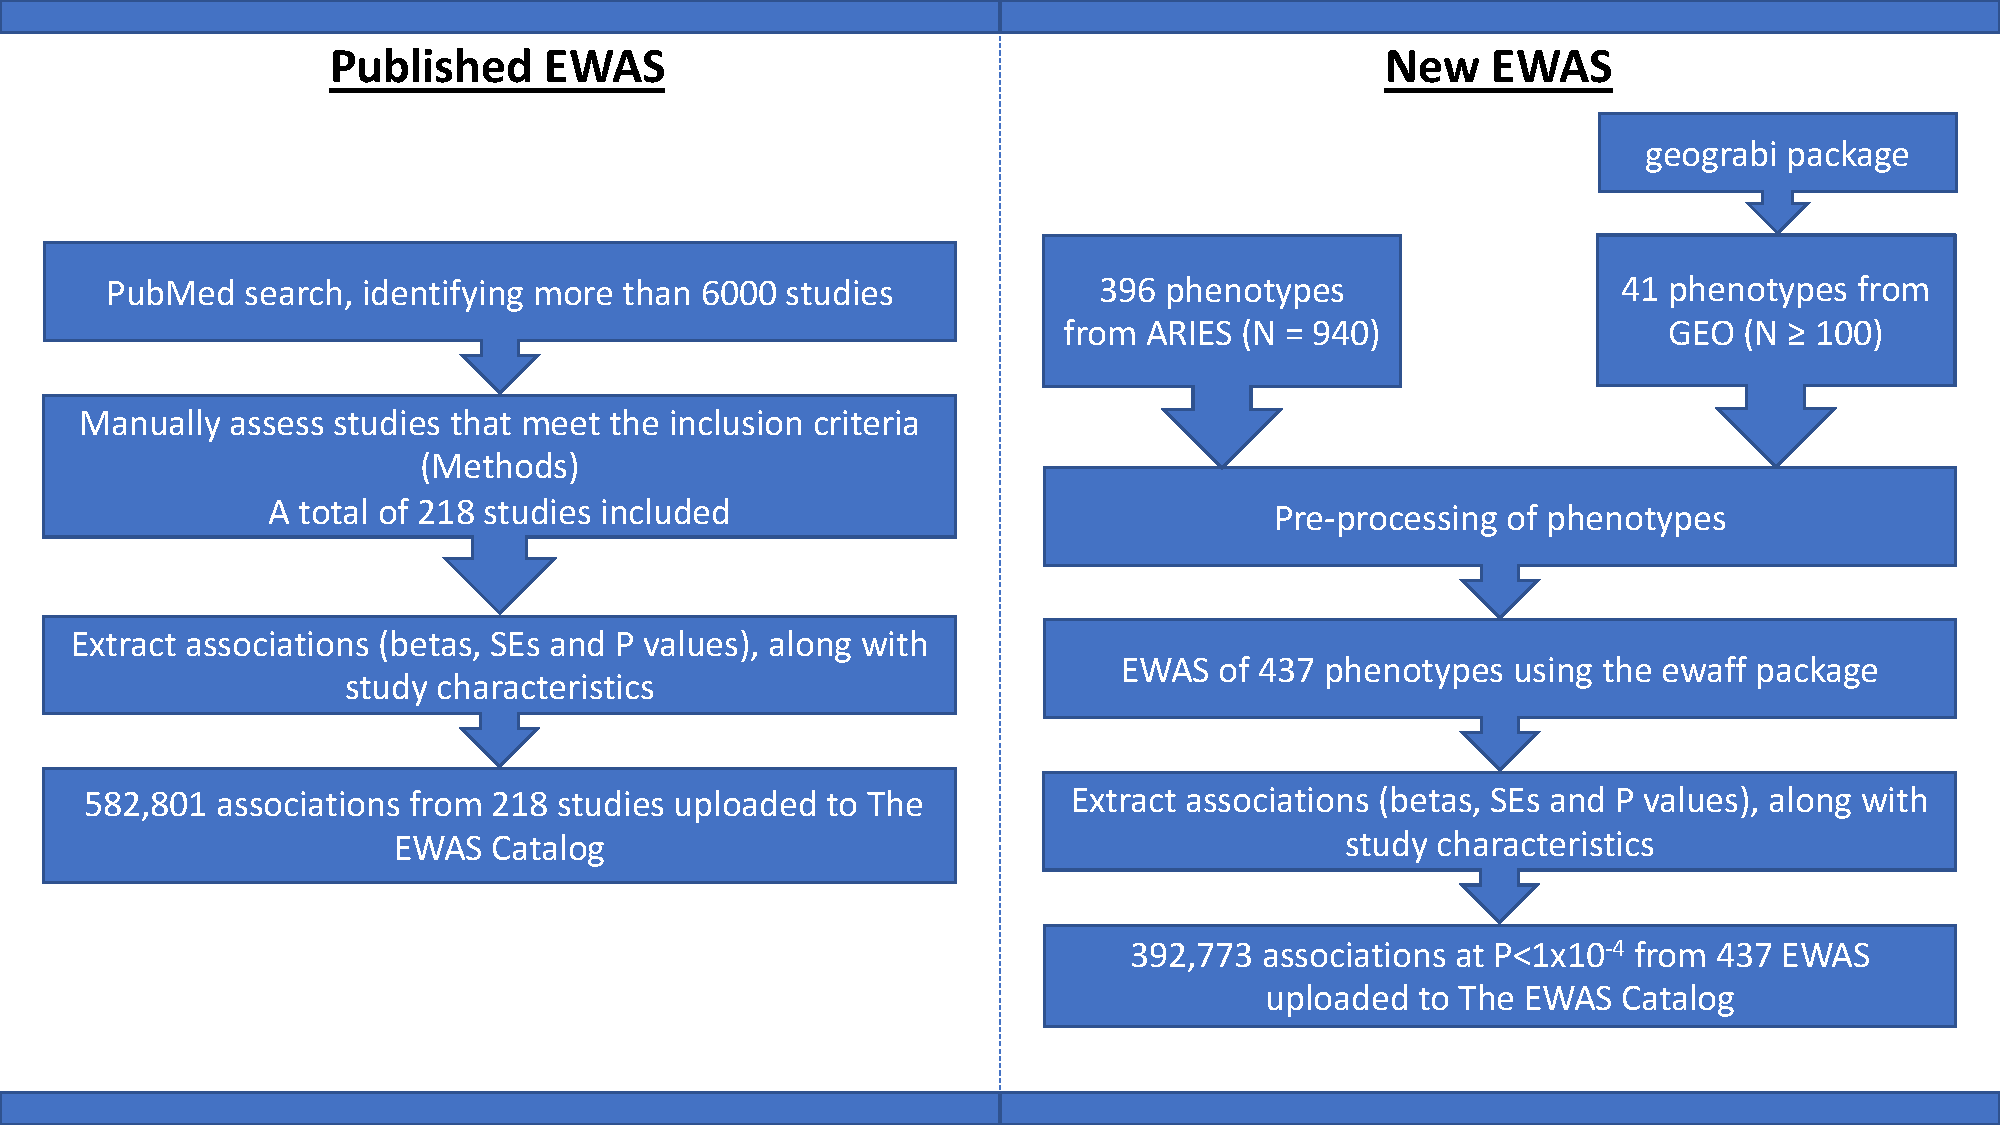
\includegraphics[width=1\linewidth]{figure/03-ewas_catalog/project_flowchart} 

}

\caption[EWAS Catalog project flowchart]{\textbf{EWAS Catalog project flowchart}. On the left is a brief description of how the CpG-phenotype associations were assembled from published works and on the right is a brief description of the EWAS performed using individual participant data.}\label{fig:catalog-project-workflow}
\end{figure}
\hypertarget{methods-03}{%
\section{Methods}\label{methods-03}}

\hypertarget{implementation}{%
\subsection{Implementation}\label{implementation}}

The EWAS Catalog web app was built using the Django Python package (\url{https://djangoproject.com}). The data is stored in a combination of MySQL databases and fast random access files (67) and can be queried via the web app or the R package (www.github.com/ewascatalog/ewascatalog-r/).

\hypertarget{overview-of-publication-data-extraction}{%
\subsection{Overview of publication data extraction}\label{overview-of-publication-data-extraction}}

To identify publications, periodic literature searches are performed in PubMed using the search terms: ``epigenome-wide'' OR ``epigenome wide'' OR ``EWAS'' OR ``genome-wide AND methylation'' OR ``genome wide AND methylation''.

To try and maximise quality and usefulness of data, and minimize computational burden, criteria for inclusion of a study into The EWAS Catalog were developed. These criteria and reasons for them are as follows:
\begin{enumerate}
\def\labelenumi{\arabic{enumi}.}
\tightlist
\item
  The EWAS performed must contain over 100 humans. Limiting the sample size to 100 or more individuals was done to try and remove EWAS that would be highly underpowered, but make sure EWAS of rarer phenotypes and in smaller cohorts (for example non-European cohorts) were not excluded.
\item
  The DNA methylation data must be genome-wide. As discussed, published candidate gene studies are at risk of publication bias and thus were excluded.
\item
  The analysis must contain over 100,000 CpG sites. Similarly to the previous criterion, this was to avoid studies performing more targeted DNA methylation measurements.
\item
  The study must include previously unpublished EWAS summary statistics. This was to prevent duplication of results.
\end{enumerate}
CpG-phenotype associations are extracted from studies at P \textless{} 1x10\textsuperscript{-4}. A P-value cutoff was imposed to avoid a large computational burden from storing millions of associations. This threshold was chosen to be more lenient than the conventional EWAS P-value threshold as there is potential information from associations reported with P-values above P \textless{} 1x10\textsuperscript{-7}, for example when trying to replicate associations in a study with a smaller sample size.

All these criteria along with the variables extracted are documented on the website (www.ewascatalog.org/documentation). Experimental factor ontology (EFO) terms were mapped to traits to unify representation of these traits. These EFO terms were manually entered after looking up the trait in the European Bioinformatics Institute database (www.ebi.ac.uk/efo).

Based on these criteria, from 2020-11-10, The EWAS Catalog contained 582,801 associations from 218 published studies.

\hypertarget{new-ewas-03}{%
\subsection{New EWAS performed}\label{new-ewas-03}}

\hypertarget{geo-data-extraction}{%
\subsubsection{Overview of GEO data extraction}\label{geo-data-extraction}}

To recruit additional datasets suitable for new EWAS analysis, the geograbi R package (\url{https://github.com/yousefi138/geograbi}) was used to both query GEO for experiments matching The EWAS Catalog inclusion criteria (described above) and extract relevant DNA methylation and phenotype information. The GEO database is briefly described in \textbf{Section \ref{geo-02}}. The query of this database was performed on 2020-10-12 and identified 136 such experiments with 32,555 samples where DNA methylation and phenotype information could be successfully extracted. From these, the aim was to repeat the analyses performed in the publications linked by PubMed IDs to each GEO record. Thus, I looked up the corresponding full texts for each dataset and identified the main variables of interest. Of the 136 putative GEO studies, only 41 (30\%) contained sufficient information to replicate the original analysis.

\hypertarget{alspac-03}{%
\subsubsection{Overview of ALSPAC data used}\label{alspac-03}}

EWAS were conducted for 387 continuous and binary traits in peripheral blood DNA methylation of ALSPAC mothers in middle age (N = 940), generated as part of the ARIES project (134). All phenotypes used in this chapter were measured at the same time blood was drawn for DNA methylation measurement. The ARIES dataset is summarised and is described in more detail in \textbf{Section \ref{aries-02}}

Ancestry principal components were used as covariates in the EWAS. These were generated within ALSPAC mothers using PLINK (v1.9). Quality control and imputation of the genetic data are described in \textbf{Section \ref{alspac-genetic-data}}. After quality control and imputation, independent SNPs (r\textsuperscript{2} \textless{} 0.01) were used to calculate the top 10 ancestry principal components.

As discussed, batch effects and cell type heterogeneity may account for a large proportion of covariation observed between DNA methylation and a phenotype of interest. In an attempt to combat this, surrogate variables were generated from the DNA methylation data using the smartsva R package (135). Surrogate variables capture variation in DNA methylation that are orthagonal to the relationship between the trait of interest and DNA methylation (85,135). When used in an EWAS model, they capture the largest portion of DNA methylation variation that is not due to the trait of interest. Thus, if batch effects and cell type heterogeneity are causing substantial variation in the DNA methylation data, this should be captured by the surrogate variables (85).

Values of continuous phenotypes were defined as outliers if greater than three multiplied by the interquartile range (IQR) or if less than three multiplied by the IQR and set to missing, then all phenotypes with 100 or more non-missing values were kept for further analysis. To ensure all phenotypes were approximately normal, each of their distributions were examined and then transformed. If a variable was deemed right-skewed, it was log-transformed then its distribution was re-assessed by eye. Square-roots and cube-roots were used to try and approximate normality if log-transformation did not work. If a variable was deemed left-skewed, it was squared, and the distribution re-assessed by eye.

\hypertarget{ewas-statistical-models}{%
\subsubsection{EWAS statistical models}\label{ewas-statistical-models}}

For all EWAS using ARIES and GEO data, linear regression models were fitted with DNA methylation at each site as the outcome and the phenotype as the exposure. DNA methylation was coded as beta values between 0 and 1. For a particular site, a beta value of 0 represents no methylation being detected in all cells measured and a value of 1 represents all cells being methylated at that site. For the 387 EWAS conducted using participant data from ARIES, covariates included age, the top 10 ancestry principal components, and 20 surrogate variables. For the 41 EWAS conducted using data extracted from GEO, just 20 surrogate variables were included as covariates. For GEO other covariates were considered, but surrogate variables only were used for two reasons: 1) to help automate the process and 2) because covariates used in the original EWAS were not included with many of the GEO datasets.

Statistical analyses were conducted in R (Version 3.6.2). The smartsva package (135) was used to create surrogate variables and the ewaff R package (\url{https://github.com/perishky/ewaff}) was used to conduct the EWAS, all p-values are two-sided.

\hypertarget{results-03}{%
\section{Results}\label{results-03}}

\hypertarget{database-interface-and-use}{%
\subsection{Database interface and use}\label{database-interface-and-use}}

There are two ways to access this large, curated database: through the main website www.ewascatalog.org or by using the R package ``ewascatalog''. The website provides a simple user interface, whereby there is one simple search bar and an advanced search bar to explore the database and links to tabs that contain documentation on the contents and how to cite its use (\textbf{Figure \ref{fig:catalog-use}}). Users may enter a CpG, gene, genome position, trait, EFO term, author name, or PudMed ID into the search bar and it will rapidly return detail for relevant EWAS associations, including CpG, trait, sample size, publication and association (effect size and P value) (\textbf{Figure \ref{fig:catalog-use}}). This information along with additional information such as ancestry, outcome, exposure units, and tissue analysed are available for download as a tab-separated value (tsv) text file. Unlike other EWAS databases, the option is provided to download summary results for both the user's search and for the entire database. Further, users may upload their own data which will be parsed by a pipeline designed to check the data and format it for input into The EWAS Catalog MySQL database.





\blandscape
\begin{figure}[htbp]

{\centering 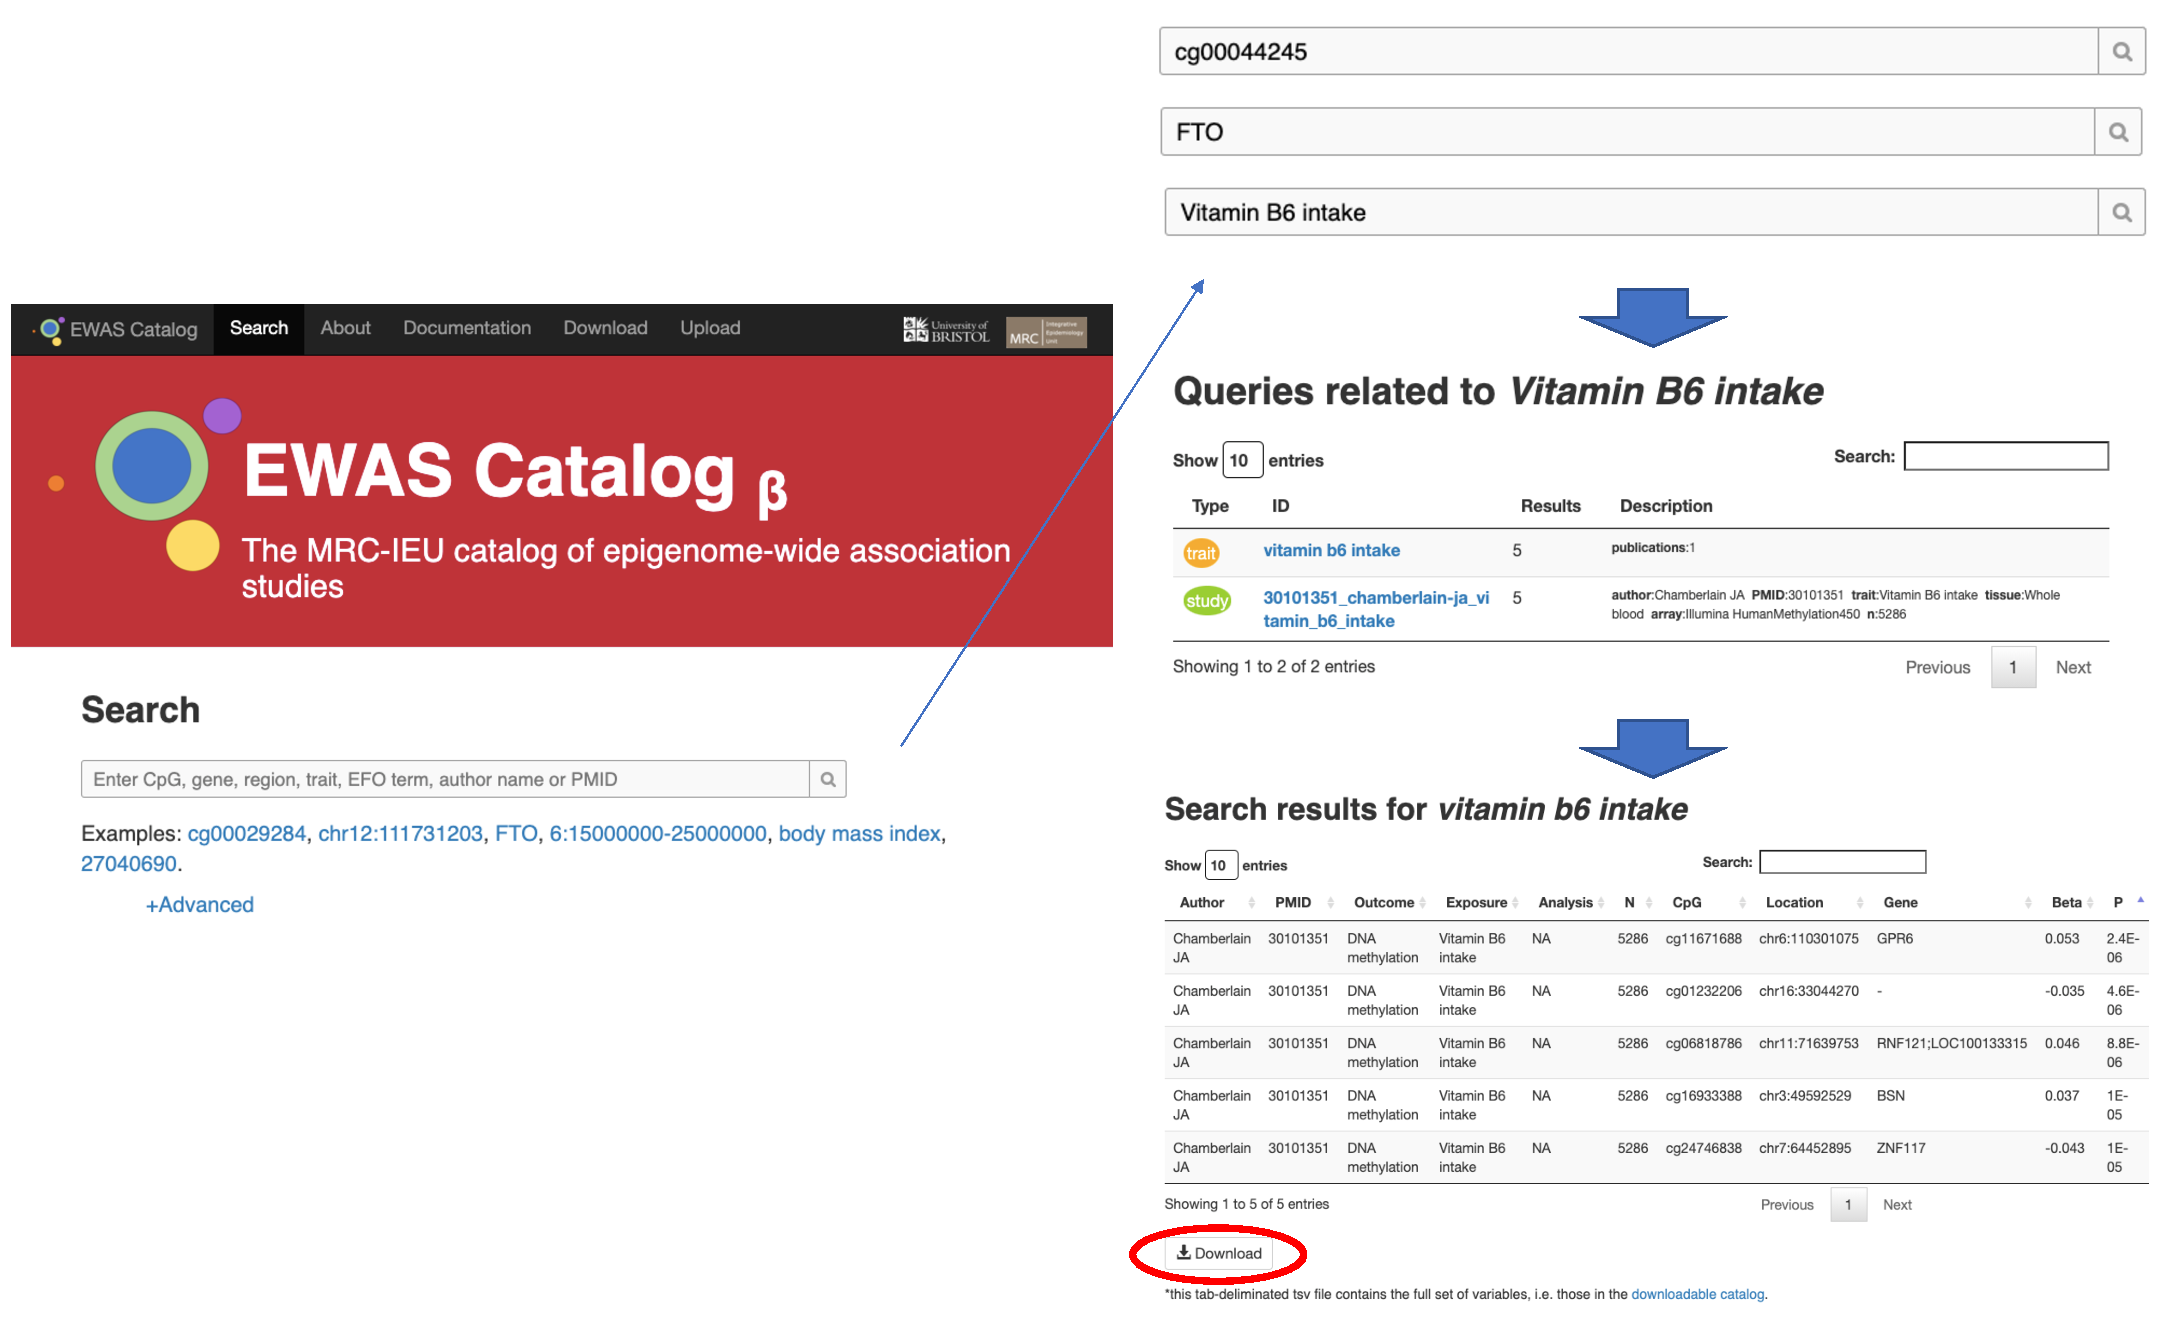
\includegraphics[width=1\linewidth]{figure/03-ewas_catalog/using_the_catalog} 

}

\caption[Using The EWAS Catalog]{\textbf{Using The EWAS Catalog}. On the left hand side is the home page. On the top right hand side are examples of searches possible: 1. CpG sites, 2. genes and 3. traits. Below the searches shows the pages directed to after searching for ``Vitamin B6 intake''. Circled in red is the download button, this button enables the user to download the results of their search as a tab-separated value file. This file will contain the information shown on the website as well as additional analysis information.}\label{fig:catalog-use}
\end{figure}
\elandscape

The R package, along with installation instructions and examples are available at \url{https://github.com/ewascatalog/ewascatalog-r/}. Once installed, the database can be queried directly in R using the ``ewascatalog()'' function similar to the website: simply supply the function with a CpG site, gene, genome position or trait and the function returns the same output as is downloadable from the website.

\hypertarget{discussion-03}{%
\section{Discussion}\label{discussion-03}}

In this chapter, a database of previously published EWAS and the full summary statistics of 428 newly performed EWAS within ALSPAC and GEO has been established. This is freely available for all researchers to use and provides a platform to explore what information has been gained from EWAS as well as a platform that can be used to pool all existing data to gain new insights into both the EWAS study itself and how DNA methylation associates with traits. Despite the fact The EWAS Atlas has similar aims to The EWAS Catalog, the latter provides full summary statistics, extra information, a user-friendly platform to enable more downstream analyses, and a pipeline for users to upload their own data and receive a citable DOI for it.

The EWAS catalog team will continue to collate and upload newly published EWAS and further increase the number of full summary statistics on the website by performing additional EWAS on available datasets and by inviting EWAS authors to provide full summary statistics. Currently work is ongoing to include additional functionality to allow users to easily and systematically compare their EWAS findings to EWAS in the database. With this full summary data, it is possible to make greater strides into discovering the epigenetic architecture of traits.

In this chapter, a platform has been generated that enables us to examine 1) what information has been gained from EWAS and 2) what could explain EWAS associations, which will be explored in \textbf{Chapter \ref{properties-of-ewas}}.

\hypertarget{contributions-statement-03}{%
\section{Contributions statement}\label{contributions-statement-03}}

Contributors and their role are listed below:
\begin{itemize}
\tightlist
\item
  James Staley produced the original website (this has since been developed by myself and Matthew Suderman).
\item
  Matthew Suderman helped re-format and develop the website
\item
  Paul Yousefi extracted GEO data
\item
  Matthew Suderman and Paul Yousefi are part of the core development team (along with myself) and continue to provide expert guidance
\item
  James Staley, Gemma Crawford, Claire Prince, Mahsa Sheikhali Babaei, Charlie Hatcher, Maria Vega Salas, Sahar Khodabakhsh, Oliver Whitehurst, Luke Mahoney all extracted some published data
\end{itemize}
\hypertarget{properties-of-ewas}{%
\chapter{Properties of epigenome-wide association studies}\label{properties-of-ewas}}

\hypertarget{chapter-summary-04}{%
\section{Chapter summary}\label{chapter-summary-04}}

The EWAS Catalog database developed in \textbf{Chapter \ref{ewas-catalog}} contains thousands of associations from hundreds of studies. By far the most common method of measuring DNA methylation amongst these EWAS is by using the Illumina Infinium HumanMethylation450 BeadChip (HM450 array). This platform assays fewer than 2\% of CpG sites in the human genome, and those selected are ascertained for regions hypothesised to be relevant to gene regulation. Understanding what drives the associations found by measuring DNA methylation in this way could help prioritise CpG sites or regions of the genome to target for future technologies used in EWAS and could guide EWAS study design.

In this chapter I use the data collected for The EWAS Catalog to evaluate the characteristics of known DNA methylation associations to determine those which increase the chance of association in EWAS. This is evaluated in three contexts. Firstly, the extent to which associations might be explained by known biases is examined. Next, individual statistical characteristics of DNA methylation (variance and heritability) are explored. Finally, analyses are performed to assess whether differentially methylated positions (DMPs) (CpGs that associate with a trait at P \textless{} 1x10\textsuperscript{-7}), are enriched for particular genomic locations.

The analyses were performed here were using data from The EWAS Catalog that was up to date as of 2019-01-01.

I performed analyses in and wrote up all sections of the work, but was helped with the enrichment analyses. A full contributions statement can be found at the end of this chapter (\textbf{Section \ref{contributions-statement-04}}).

\hypertarget{introduction-04}{%
\section{Introduction}\label{introduction-04}}

Hundreds of EWAS have been conducted in the last 10-15 years, yet no systematic evaluation of published EWAS across complex traits has been conducted. By exploring the patterns of association across a large group of EWAS, one can discover potential explanations for the results found, that may shed light on technical issues affecting previous studies as well as shared epigenetic architectures across traits.

Since the inception of EWAS, it has become clear that batch effects and cellular heterogeneity can generate false positives and bias effect sizes (2,79,82). Also, as discussed in \textbf{Section \ref{measuring-dna-methylation}}, characterisation of probes used by common arrays (e.g.~the HM450 array and the HMEPIC array) has shown that unreliable methylation measurements may occur because of cross-hybridisation of probes, non-specific probe mapping and SNPs being present at the binding sites of probes (83,84). Despite this, there are examples of replication amongst EWAS results, (104,136--141). Further funcitonal characterisation of EWAS results, such as new experimental studies or the application of existing gene function knowledge, can also be used to bolster evidence that changes in DNA methylation estimated are unlikely due to bias (66,142). By way of an example, changes in DNA methylation at \emph{AHRR} have been replicated across multiple smoking EWAS (68,104,105,143) and as functional reaseach has implicated this gene in handling toxic substances found in tobacco smoke (144), it seems unlikely these findings are chance occurances.

The characteristics of the DNA methylome may also explain some EWAS findings. Heritability varies across DNA methylation sites (145,146), and so if genetic effects are driving EWAS associations, either through confounding or with DNA methylation as a mediator, one would expect heritable sites to be commonly identified in EWAS. Variance is also heterogenous across sites (147) and at sites where variation is low, the ratio of noise to signal may be greater. Thus, some studies have advocated removing these sites to prevent generating false positives and to reduce the multiple testing burden (131,148). However, it is unclear how variance in DNA methylation relates to the magnitude of effect estimates.

Experimental studies have shown DNA methylation changes at different locations of the genome correlate with different regulatory functions. For example, an increase in DNA methylation at transcriptional start sites is correlated with a decrease in gene expression (18,33,34), but an increase in DNA methylation within a gene body shows the opposite association (35,36). As discussed in \textbf{Section \ref{ewas}}, the understanding that the genomic contexts in which DNA methylation occurs is related to gene regulation likely contributed to the design of contemporary arrays that measure DNA methylation. Yet, it is not known whether targeting protein-coding regions and enhancers has likely led to an increase in discovery of DNA methylation-trait assocaitions.

Understanding underlying factors that drive EWAS results is essential for future study design. This may come in the form of consideration of potential biasing factors, or by selecting certain DNA methylation sites based on their specific characteristics. Further, the HM450 and HMEPIC arrays both capture less than 5\% of the total number of CpG sites in the genome, therefore understanding the characteristics of DNA methylation-trait associations and could provide vital information when designing future technologies targeting the other 95\%.

Also, by examining the commonalities of EWAS results, one has the potential to uncover links between traits that have not previously been made or to identify new potential mediating factors between traits.

In this chapter I first describe the data present in The EWAS Catalog going on to explore the factors that predict EWAS hits.

\newpage

\hypertarget{methods-04}{%
\section{Methods}\label{methods-04}}

\hypertarget{ewas-data-04}{%
\subsection{Epigenome-wide association studies data}\label{ewas-data-04}}

All the data for the analyses were extracted from The EWAS Catalog (\textbf{Chapter \ref{ewas-catalog}}). Data were extracted when The EWAS Catalog had published EWAS data from before the start of 2019 (i.e.~the data do not completely reflect that presented in \textbf{Chapter \ref{ewas-catalog}}). Studies were removed that compared DNA methylation levels between tissue, race, and age. This was done because these variables are not complex traits and thus the properties of those study results are unlikely to be informative when attempting to understand how to best design EWAS. Overall, this left 614 EWAS, including 387 EWAS from the ARIES subsection of ALSPAC (\textbf{Section \ref{aries-02}}) (126,127,134) and 40 EWAS performed using data from the gene expression omnibus (GEO) resource (\textbf{Section \ref{geo-02}}). See \textbf{Chapter \ref{ewas-catalog}} for more details on the EWAS.

\hypertarget{description-of-data}{%
\subsection*{Description of catalog data}\label{description-of-data}}
\addcontentsline{toc}{subsection}{Description of catalog data}

DMPs, unless otherwise stated, will be defined as DNA methylation sites associated with a trait at P \textless{} 1x10\textsuperscript{-7}. Each of the CpGs in the Catalog are annotated to genes, using data from the meffil R package (149).

T-statistics (\(t\)) were calculated using P-values, sample sizes (\(n\)) and the qt() function in R. \(r^2\) values were calculated from t-statistics as follows
\begin{equation}
    r^2 = \frac{t^2} {t^2 + n - 1}
    \label{eq:r-squared}
\end{equation}
Traits for which r\textsuperscript{2} values might be inflated were identified. For each EWAS the estimated r\textsuperscript{2} values were summed, divided by the sample size (N) of the analysis and the base 10 log of these values taken to approximate a normal distribution. Then a z-test was performed to assess for which studies the sum of r\textsuperscript{2} values divided by N were greater than the mean of summed r\textsuperscript{2} values divided by N across all studies. From the z-test, those with a FDR-corrected P-value of less than 0.05 were labelled as having inflated r\textsuperscript{2} values.

\hypertarget{identifying-faulty-probes}{%
\subsection{Identifying faulty probes}\label{identifying-faulty-probes}}

By far the most common method to measure DNA methylation across the studies in The EWAS Catalog is using the HM450 array. Since its development, the array has been extensively characterised (2,79,82,83) and it was found not all probes measure DNA methylation reliably. Some probes map to CpG sites that are influenced by SNPs, others are non-specific and some are prone to cross-hybridisation. Probes were assigned to be `potentially faulty' if they were characterised as such by Zhou et al.~(83).

\hypertarget{replication-methods-04}{%
\subsection{Replication}\label{replication-methods-04}}

A study-wide significant association (P\textless1x10\textsuperscript{-7}) was deemed to be replicated if it had been identified by another study at P\textless1x10\textsuperscript{-4}. It should be re-iterated that the published data collected for The EWAS Catalog was scraped from the journal articles and there is heterogeneity in reporting of EWAS associations. Therefore, some studies would not have reported any results with a P-value lower than the conventional EWAS P-value threshold (P\textless1x10\textsuperscript{-7}), making power a key limitation for attempts to assess replication. The replicability of EWAS within the database was assessed using two methods. Firstly, replication within studies is recorded in the EWAS Catalog, thus a simple lookup for any studies that performed a replication or meta-analysed discovery and replication datasets was conducted. Secondly, a lookup of results for any traits for which multiple EWAS had been conducted was performed.

The Catalog also contains results from studies that have uploaded their data to GEO as well as results from the re-analysis of that data (details in \textbf{Section \ref{new-ewas-03}}). These re-analyses adjusted for 20 surrogate variables only as many studies did not provide a complete set of covariates to GEO. A lookup in the re-analysed data for results found in the original EWAS was performed.

\hypertarget{selecting-data-to-assess-dna-methylation-characteristics}{%
\subsection{Selecting data to assess DNA methylation characteristics}\label{selecting-data-to-assess-dna-methylation-characteristics}}

Before further analyses, all potentially faulty probes and probes that mapped to sex chromomsomes were removed, studies that did not include batch and cell composition as covariates in at least one EWAS model were excluded, and studies for which re-analysis of the data replicated less than 10\% of the findings were removed.

\hypertarget{dna-methylation-characteristics}{%
\subsection{DNA methylation characteristics}\label{dna-methylation-characteristics}}

The relationship between heritability and variance of DNA methylation at each CpG site and EWAS effect size was assessed. To allow this across traits, beta coefficients were standardised, \(\beta_{standard}\), like so,
\begin{equation}
    \beta_{standard} = \frac{\beta\sigma(x)} {\sigma(y)}
    \label{eq:standardised-beta-coeffs}
\end{equation}
where \(\beta\) = beta coefficient, \(\sigma\) = the standard deviation. As individual participant data were not available to us, the variance in DNA methylation sites was approximated by the variance in DNA methylation at sites as supplied by the GoDMC (150) and the trait variance was estimated by rearranging equation \eqref{eq:r-squared-from-beta} depending on whether DNA methylation was the independent (\(x\)) or dependent (\(y\)) variable in the model.
\begin{equation}
    r^2 = \frac{\beta^2\sigma^2(x)} {\sigma^2(y)}
    \label{eq:r-squared-from-beta}
\end{equation}
GoDMC (150) also provided the mean levels of DNA methylation at each site. Heritability of DNA methylation at each site has been previously estimated by McRae et al.~2014 (145) and Van Dongen et al.~2016 (151). These values were kindly made publically available by the authors of those studies in this chapter the estimates of heritability from twin data (Van Dongen et al.~2016 (151)) were used.

Relationships between each characteristic and effect size were assessed using linear regression, fitting the absolute value of the standardised effect size as the dependent variable and the characteristic as the independent variable. The absolute values of standardised effect sizes were transformed using the natural log to approximate normality.

The relationship between tendancy for a DMP to replicate and heritability and variance were also assessed. Logistic regression models were fitted with the binary variable of a DMP replicating in at least one study (yes or no) used as the outcome measure and heritability and variance fitted as the dependent variable.

It was also tested whether heritability and variance could predict whether a CpG site was likely to be identified as a DMP in EWAS by generating receiver operator characteristic (ROC) curves and quantifying the area under these curves (AUC).

\hypertarget{enrichment-tests-04}{%
\subsection{Enrichment tests}\label{enrichment-tests-04}}

Assessment of enrichment of DMPs amongst various genomic regions was carried out to help understand whether selecting regions to measure could maximise EWAS yield. Locus Overlap Analysis (LOLA) (152) was used to assess whether DMPs identified in the EWAS Catalog were enriched for 25 chromatin states and 167 transcription factor binding sites in 127 different cell types comprising 25 distinct tissues. These data were generated by the Roadmap Epigenomics Project (153) and ENCODE (154).

Five different groups of DMPs were defined for the enrichment analyses:
\begin{itemize}
\tightlist
\item
  Group A - all sites associated with any complex trait at the conventional P-value threshold used in EWAS, P \textless{} 1x10\textsuperscript{-7}.
\item
  Group B - a subset of group A, all sites associated with any complex trait at a more stringent threshold, P \textless{} 1.6e-10. Multiple EWAS were conducted to produce the results in the database and so the stricter threshold of group B aimed to limit the false discovery rate by taking into account the multiple EWAS.
\item
  Group C - DMPs replicated at P \textless{} 1x10\textsuperscript{-4} in any other EWAS of the same trait.
\item
  Group D - a subset of group A, but restricted to results from studies where DNA methylation was measured in whole blood.
\item
  Group E - a subset of group B, but restricted to results from studies where DNA methylation was measured in whole blood.
\end{itemize}
To assess enrichment, LOLA performs Fisher's exact test and generates an odds ratio that can be interpreted as the odds of the DMPs being within an annotation divided by the odds of the DMPs not being within an annotation. Genomic annotations may differ by CG content and thus a differential CG content of regions containing the DMPs of interest and the background group of CpG sites might bias enrichment estimates. Thus, background sites were matched on CG content before the analysis.

All analyses were completed using R (version 3.6.2).

\newpage

\hypertarget{results-04}{%
\section{Results}\label{results-04}}

\hypertarget{catalog-description}{%
\subsection*{Description of the catalog}\label{catalog-description}}
\addcontentsline{toc}{subsection}{Description of the catalog}

Before assessing the factors predicting DMPs, a brief summary of the data in The EWAS Catalog (as used for this study, see \textbf{Section \ref{ewas-data-04}} for details) is presented (\textbf{Table \ref{tab:study-data-tab}}). \linebreak
\begin{table}[!h]

\caption{\label{tab:study-data-tab}Description of data present in the EWAS Catalog}
\centering
\resizebox{\linewidth}{!}{
\begin{tabular}[t]{ll}
\toprule
study-trait & value\\
\midrule
\cellcolor{gray!6}{Number of EWAS} & \cellcolor{gray!6}{614}\\
Unique traits & 556\\
\cellcolor{gray!6}{Number of samples} & \cellcolor{gray!6}{389527}\\
Median sample size (range) & 536 (93 - 13474)\\
\cellcolor{gray!6}{Number of associations} & \cellcolor{gray!6}{155976}\\
\addlinespace
Unique CpGs identified & 129670\\
\cellcolor{gray!6}{Unique genes identified} & \cellcolor{gray!6}{19305}\\
Sex (\%) & Both (38.6), Females (52.0), Males (2.1)\\
\cellcolor{gray!6}{Ethnicities} & \cellcolor{gray!6}{EUR (75.3), Unclear (12.5), AFR (4.6), Other (3.6), ADM (1.6), EAS (1.4), SAS (1.0)}\\
Age (\%) & Adults (72.5), Geriatrics (11.2), Children (4.9), Infants (4.4)\\
\addlinespace
\cellcolor{gray!6}{Number of tissue types} & \cellcolor{gray!6}{42}\\
Most common tissues (\%) & whole blood (84.14), cord blood (4.34), cd4+ t-cells (2.60), placenta (1.24), saliva (0.99)\\
\bottomrule
\multicolumn{2}{l}{\textsuperscript{} Identified associations were defined as those P < 1x10\textsuperscript{-7}}\\
\multicolumn{2}{l}{\textsuperscript{} Results for Sex, Ethnicities, Age, and Most common tissues were calculated per EWAS. So if one EWAS (or meta-analysis) contained just}\\
\multicolumn{2}{l}{Afican indviduals then that would be counted as one}\\
\end{tabular}}
\end{table}
\linebreak

The percentage of hypermethylated sites in relation to traits was 52\% and there were five CpGs that associated with more than ten traits (\textbf{Figure \ref{fig:traits-manhattan}}). Here are those sites with gene names, as mapped using Illumina-provided annotations, in brackets: cg01940273 (\emph{-}), cg05575921 (\emph{AHRR}), cg00574958 (\emph{CPT1A}), cg17901584 (\emph{DHCR24}), cg06500161 (\emph{ABCG1}). cg06500161 (\emph{ABCG1}) was associated with more traits than any other site - 71 traits. These correspond mostly to metabolites, weight-related traits, and type two diabetes.




\begin{figure}

{\centering \includegraphics[width=1\linewidth]{figure/04-properties_of_ewas/traits_per_dmp_at_1e-07} 

}

\caption[Number of unique traits associated with DNA methylation at each CpG]{\textbf{Number of unique traits associated with DNA methylation at each CpG}. Sites associated with more than 10 unique traits are highlighted in orange and labelled.}\label{fig:traits-manhattan}
\end{figure}
Next we estimated the trait variance (see equation \eqref{eq:r-squared}) explained by each association. This indicates the predictive performance from EWAS, although it should be noted that winner's curse will artificially inflate the performance, even amongst EWAS with true positive results.

The proportion of trait variance (ranging from 0 to 1) that correlated with DNA methylation (r\textsuperscript{2}) at each site varied from 0.0011 to 0.97 with a median of 0.093 (\textbf{Figure \ref{fig:rsq-distribution}}). The sum of r\textsuperscript{2} values ranged greatly from 0.0055 to 23,879 (\textbf{Figure \ref{fig:rsq-sum-distribution}}), with a median of 1.2. There was evidence that 54 studies had a total sum of r\textsuperscript{2} values greater than the mean (FDR \textless{} 0.05) and r\textsuperscript{2} values from individual associations from these studies made up the majority of r\textsuperscript{2} values greater than 0.1 (\textbf{Figure \ref{fig:rsq-distribution}}). When excluding those studies from the results, the median r\textsuperscript{2} value at individual sites was 0.023.




\begin{figure}

{\centering 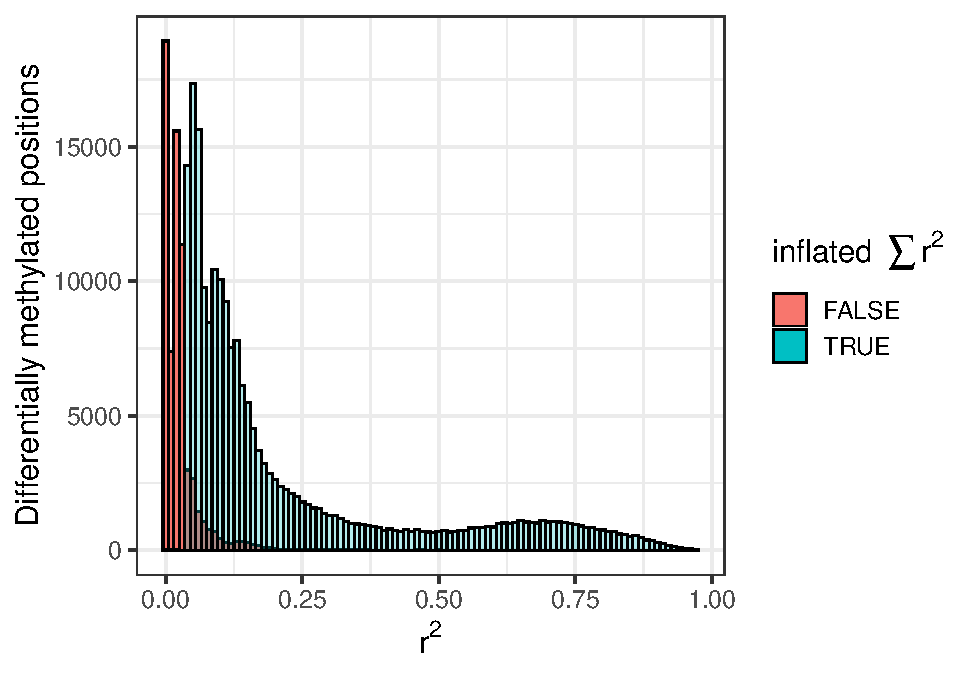
\includegraphics[width=1\linewidth]{thesis_files/figure-latex/rsq-distribution-1} 

}

\caption[Distribution of r\textsuperscript{2} values across all CpG sites in The EWAS Catalog]{\textbf{Distribution of r\textsuperscript{2} values across all CpG sites in The EWAS Catalog}. Each EWAS can identify multiple differentially methylated positions, each of which will capture some variance of the trait of interest for that EWAS (r\textsuperscript{2}). \(\sum {r^2}\) is the sum of r\textsuperscript{2} values, the distribution of which is shown in \textbf{Figure \ref{fig:rsq-sum-distribution}}. Fifty-four studies were identified for which there was some evidence that the sum of r\textsuperscript{2} values were greater than the mean across all studies. All of the differentially methylated positions identified by those studies are highlighted in blue on the plot.}\label{fig:rsq-distribution}
\end{figure}



\begin{figure}

{\centering 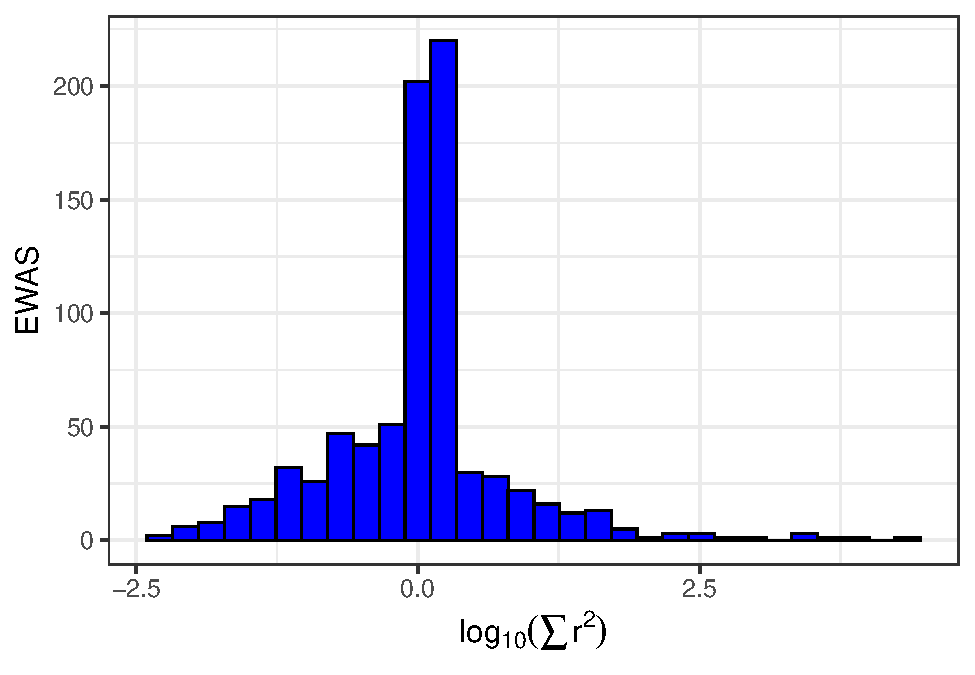
\includegraphics[width=1\linewidth]{thesis_files/figure-latex/rsq-sum-distribution-1} 

}

\caption[Distribution of the sum of r\textsuperscript{2} values across each study in The EWAS Catalog]{\textbf{Distribution of the sum of r\textsuperscript{2} values across each study in The EWAS Catalog}.}\label{fig:rsq-sum-distribution}
\end{figure}
These results suggest that some associations within the database are likely to be inflated, yet for most traits, variation at individual DNA methylation sites captures little trait variance. Summing the r\textsuperscript{2} values indicates a substantial proportion of trait variance can be captured by multiple DNA methylation sites for some traits, but this can only be estimated by jointly modelling the contribution of all sites to trait variance. This is explored in \textbf{Chapter \ref{h2ewas-chapter}}. Here, the sum of r\textsuperscript{2} values is used to indicate whether the results of a study are likely inflated and thus may not be reliable.

\hypertarget{robustness-of-results}{%
\subsection{Robustness of results}\label{robustness-of-results}}

As discussed, cellular heterogeneity, batch effects and inclusion of faulty probes can lead to false positives in EWAS. The extent to which this might be the case within EWAS included within The EWAS Catalog was explored.

Each study may have reported results across multiple EWAS models, adjusting for different covariates. In at least one model, 579 studies adjusted for batch effects, 518 studies adjusted for cell composition, and 489 adjusted for both. Of all DMPs identifed, 9.3\% were measured by potentially faulty probes and an extra 0.64\% were present on sex chromosomes (\textbf{Figure \ref{fig:faulty-probes-plot}}).




\begin{figure}

{\centering 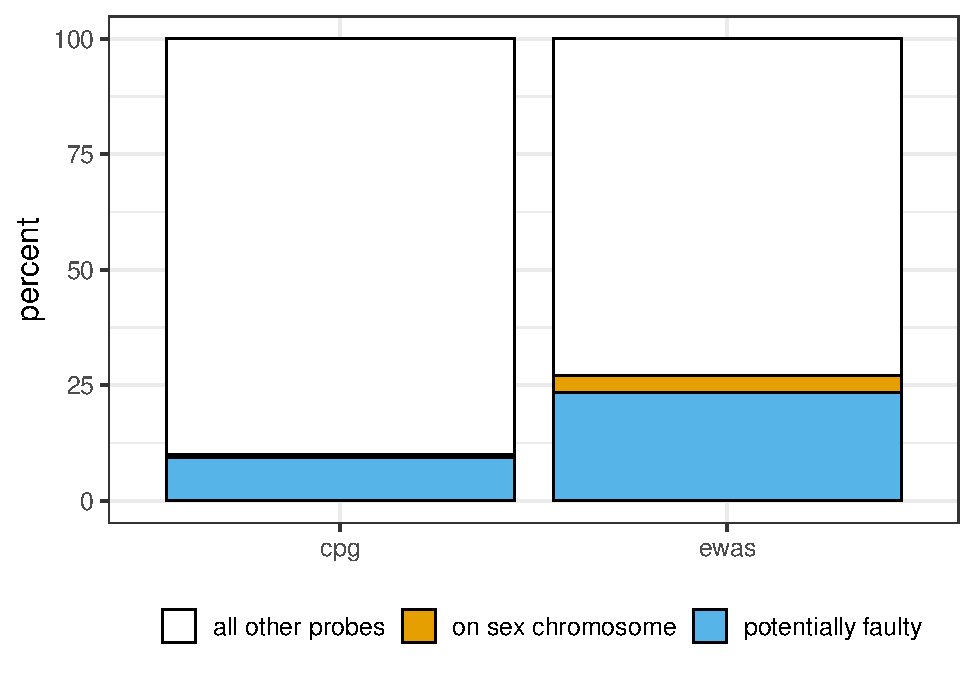
\includegraphics[width=1\linewidth]{thesis_files/figure-latex/faulty-probes-plot-1} 

}

\caption[The percentage of DMPs that may have been identified by faulty probes and the percentage of EWAS that reported identifying at least one of these probes]{\textbf{The percentage of DMPs that may have been identified by faulty probes and the percentage of EWAS that reported identifying at least one of these probes}. The left-hand bar represents all DMPs reported across all EWAS that fit into the categories shown, the right-hand bar represents the number of EWAS that include CpGs that fit into the categories shown. Some CpGs are both on a sex chromosome and were identified as faulty by Zhou et al.~They were labelled as `potentially faulty'.}\label{fig:faulty-probes-plot}
\end{figure}
There were 30 studies that performed a meta-analysis of discovery and replication samples. A further 48 studies performed a separate replication analysis. Together, this provides 1666 associations within the EWAS Catalog that have been replicated at P \textless{} 1x10\textsuperscript{-4}.

From the studies that uploaded their data to GEO, the association between DNA methylation and the phenotype of interest from the original study was re-analysed, including 20 surrogate variables as covariates. Both the original study results and the results from the re-analysis of the phenotype of interest are in The EWAS Catalog database for 9 studies. Across the studies, between 0\% and 96.875\% of DMPs were replicated at P \textless{} 1x10\textsuperscript{-4} (\textbf{Table \ref{tab:geo-reanalysis-tab}}). Some of these EWAS reported very few DMPs (some only 1) and as they would have used different models, replicating the single reported result was not expected. \linebreak
\begin{table}[!h]

\caption{\label{tab:geo-reanalysis-tab}GEO re-analysis replication}
\centering
\resizebox{\linewidth}{!}{
\begin{tabular}[t]{llll}
\toprule
Trait & N-DMPs & N-replicated & Percent-replicated\\
\midrule
\cellcolor{gray!6}{Age at menarche} & \cellcolor{gray!6}{1} & \cellcolor{gray!6}{0} & \cellcolor{gray!6}{0.00}\\
Arsenic exposure & 12 & 0 & 0.00\\
\cellcolor{gray!6}{Fetal alcohol spectrum disorder} & \cellcolor{gray!6}{19} & \cellcolor{gray!6}{1} & \cellcolor{gray!6}{5.26}\\
Inflammatory bowel disease & 14 & 13 & 92.86\\
\cellcolor{gray!6}{Nevus count} & \cellcolor{gray!6}{1} & \cellcolor{gray!6}{0} & \cellcolor{gray!6}{0.00}\\
\addlinespace
Psoriasis & 16 & 0 & 0.00\\
\cellcolor{gray!6}{Rheumatoid arthritis} & \cellcolor{gray!6}{47,875} & \cellcolor{gray!6}{116} & \cellcolor{gray!6}{0.24}\\
Smoking & 32 & 31 & 96.88\\
\cellcolor{gray!6}{Smoking} & \cellcolor{gray!6}{30} & \cellcolor{gray!6}{12} & \cellcolor{gray!6}{40.00}\\
\bottomrule
\multicolumn{4}{l}{\textsuperscript{} N-DMPs = number of differentially methylated positions}\\
\multicolumn{4}{l}{identified at P < 1x10\textsuperscript{-7}}\\
\multicolumn{4}{l}{\textsuperscript{} N-replicated = number of DMPs replicated in the GEO}\\
\multicolumn{4}{l}{re-analysis at P < P < 1x10\textsuperscript{-4}}\\
\end{tabular}}
\end{table}
\linebreak

Using the catalog data, DMPs were examined to see if they were also associated with that same trait in another study at P\textless1x10\textsuperscript{-4}. There were 72 studies that shared a common phenotype of interest. Replication rate, judged as the percentage of CpGs also present in any other study of the same trait with P\textless1x10\textsuperscript{-4}, varied from 0 to 100 between studies (\textbf{Table \ref{tab:replication-tab}}, \textbf{Table \ref{tab:replication-tab-smoking}}, \textbf{Table \ref{tab:replication-tab-bmi}}). For many of the traits, the number of identified DMPs was low (0 studies reported one DMP), therefore the low replication rate for these studies is not completely unexpected given potential study heterogeneity in important factors such as study power, age, sex, ancestry and study design. However, there were also three studies that identified over 100 DMPs and none of them replicated, including an EWAS of smoking for which there are many high-powered replication studies. \linebreak
\begin{table}

\caption{\label{tab:replication-tab}Replication rate}
\centering
\resizebox{\linewidth}{!}{
\begin{tabular}[t]{lllll}
\toprule
Trait & N-DMPs & N-replicated & N-replication-studies & Prop-replicated\\
\midrule
\cellcolor{gray!6}{glucose} & \cellcolor{gray!6}{4} & \cellcolor{gray!6}{1} & \cellcolor{gray!6}{1} & \cellcolor{gray!6}{0.25000}\\
insulin & 3 & 1 & 2 & 0.33333\\
\cellcolor{gray!6}{insulin} & \cellcolor{gray!6}{1} & \cellcolor{gray!6}{0} & \cellcolor{gray!6}{2} & \cellcolor{gray!6}{0.00000}\\
alzheimers & 21 & 5 & 1 & 0.23810\\
\cellcolor{gray!6}{alzheimers} & \cellcolor{gray!6}{25} & \cellcolor{gray!6}{7} & \cellcolor{gray!6}{1} & \cellcolor{gray!6}{0.28000}\\
\addlinespace
Birth weight & 27 & 0 & 4 & 0.00000\\
\cellcolor{gray!6}{Birth weight} & \cellcolor{gray!6}{1} & \cellcolor{gray!6}{0} & \cellcolor{gray!6}{4} & \cellcolor{gray!6}{0.00000}\\
Birth weight & 2 & 0 & 4 & 0.00000\\
\cellcolor{gray!6}{Triglycerides} & \cellcolor{gray!6}{4} & \cellcolor{gray!6}{2} & \cellcolor{gray!6}{3} & \cellcolor{gray!6}{0.50000}\\
Triglycerides & 11 & 6 & 3 & 0.54545\\
\addlinespace
\cellcolor{gray!6}{Triglycerides} & \cellcolor{gray!6}{33} & \cellcolor{gray!6}{26} & \cellcolor{gray!6}{3} & \cellcolor{gray!6}{0.78788}\\
Triglycerides & 1 & 1 & 3 & 1.00000\\
\cellcolor{gray!6}{Waist circumference} & \cellcolor{gray!6}{172} & \cellcolor{gray!6}{6} & \cellcolor{gray!6}{2} & \cellcolor{gray!6}{0.03488}\\
Waist circumference & 11 & 3 & 2 & 0.27273\\
\cellcolor{gray!6}{Waist circumference} & \cellcolor{gray!6}{2} & \cellcolor{gray!6}{1} & \cellcolor{gray!6}{2} & \cellcolor{gray!6}{0.50000}\\
\addlinespace
Type II diabetes & 11 & 2 & 2 & 0.18182\\
\cellcolor{gray!6}{Type II diabetes} & \cellcolor{gray!6}{6} & \cellcolor{gray!6}{0} & \cellcolor{gray!6}{2} & \cellcolor{gray!6}{0.00000}\\
Type II diabetes & 1 & 1 & 2 & 1.00000\\
\cellcolor{gray!6}{HOMA-IR} & \cellcolor{gray!6}{1} & \cellcolor{gray!6}{1} & \cellcolor{gray!6}{1} & \cellcolor{gray!6}{1.00000}\\
HOMA-IR & 5 & 1 & 1 & 0.20000\\
\addlinespace
\cellcolor{gray!6}{Schizophrenia} & \cellcolor{gray!6}{3} & \cellcolor{gray!6}{0} & \cellcolor{gray!6}{2} & \cellcolor{gray!6}{0.00000}\\
Schizophrenia & 163 & 0 & 2 & 0.00000\\
\cellcolor{gray!6}{C-reactive protein} & \cellcolor{gray!6}{3} & \cellcolor{gray!6}{3} & \cellcolor{gray!6}{1} & \cellcolor{gray!6}{1.00000}\\
C-reactive protein & 226 & 17 & 1 & 0.07522\\
\cellcolor{gray!6}{High-density lipoprotein cholesterol} & \cellcolor{gray!6}{2} & \cellcolor{gray!6}{2} & \cellcolor{gray!6}{1} & \cellcolor{gray!6}{1.00000}\\
\addlinespace
High-density lipoprotein cholesterol & 63 & 5 & 1 & 0.07937\\
\cellcolor{gray!6}{Serum high-density lipoprotein cholesterol} & \cellcolor{gray!6}{22} & \cellcolor{gray!6}{17} & \cellcolor{gray!6}{1} & \cellcolor{gray!6}{0.77273}\\
Serum high-density lipoprotein cholesterol & 213 & 11 & 1 & 0.05164\\
\cellcolor{gray!6}{Serum low-density lipoprotein cholesterol} & \cellcolor{gray!6}{61} & \cellcolor{gray!6}{0} & \cellcolor{gray!6}{1} & \cellcolor{gray!6}{0.00000}\\
Serum total cholesterol & 1 & 0 & 2 & \vphantom{1}0.00000\\
\addlinespace
\cellcolor{gray!6}{Serum total cholesterol} & \cellcolor{gray!6}{111} & \cellcolor{gray!6}{0} & \cellcolor{gray!6}{2} & \cellcolor{gray!6}{0.00000}\\
Serum total cholesterol & 1 & 0 & 2 & 0.00000\\
\cellcolor{gray!6}{Serum triglycerides} & \cellcolor{gray!6}{46} & \cellcolor{gray!6}{38} & \cellcolor{gray!6}{1} & \cellcolor{gray!6}{0.82609}\\
Serum triglycerides & 99 & 33 & 1 & 0.33333\\
\cellcolor{gray!6}{Rheumatoid arthritis} & \cellcolor{gray!6}{47,875} & \cellcolor{gray!6}{8} & \cellcolor{gray!6}{1} & \cellcolor{gray!6}{0.00017}\\
\addlinespace
Rheumatoid arthritis & 6 & 0 & 1 & 0.00000\\
\cellcolor{gray!6}{Depression} & \cellcolor{gray!6}{1} & \cellcolor{gray!6}{0} & \cellcolor{gray!6}{1} & \cellcolor{gray!6}{0.00000}\\
Depression & 2 & 0 & 1 & 0.00000\\
\bottomrule
\multicolumn{5}{l}{\textsuperscript{} N-DMPs = number of differentially methylated positions identified at}\\
\multicolumn{5}{l}{P<1x10\textsuperscript{-7}}\\
\multicolumn{5}{l}{\textsuperscript{} N-replicated = number of DMPs replicated in the GEO re-analysis at}\\
\multicolumn{5}{l}{P<1x10\textsuperscript{-4}}\\
\multicolumn{5}{l}{\textsuperscript{} N-replication-studies = number of studies for which replication was examined}\\
\multicolumn{5}{l}{\textsuperscript{} Prop-replicated = proportion of DMPs replicated.}\\
\end{tabular}}
\end{table}
\begin{table}

\caption{\label{tab:replication-tab-smoking}Replication rate in EWAS of smoking}
\centering
\resizebox{\linewidth}{!}{
\begin{tabular}[t]{lllll}
\toprule
Trait & N-DMPs & N-replicated & N-replication-studies & Prop-replicated\\
\midrule
\cellcolor{gray!6}{smoking} & \cellcolor{gray!6}{1} & \cellcolor{gray!6}{1} & \cellcolor{gray!6}{21} & \cellcolor{gray!6}{\vphantom{2}1.00000}\\
smoking & 1 & 1 & 21 & \vphantom{1}1.00000\\
\cellcolor{gray!6}{smoking} & \cellcolor{gray!6}{10} & \cellcolor{gray!6}{10} & \cellcolor{gray!6}{21} & \cellcolor{gray!6}{1.00000}\\
smoking & 1,065 & 862 & 21 & 0.80939\\
\cellcolor{gray!6}{smoking} & \cellcolor{gray!6}{1} & \cellcolor{gray!6}{1} & \cellcolor{gray!6}{21} & \cellcolor{gray!6}{1.00000}\\
\addlinespace
smoking & 22 & 20 & 21 & 0.90909\\
\cellcolor{gray!6}{smoking} & \cellcolor{gray!6}{30} & \cellcolor{gray!6}{9} & \cellcolor{gray!6}{21} & \cellcolor{gray!6}{0.30000}\\
smoking & 44 & 42 & 21 & 0.95455\\
\cellcolor{gray!6}{smoking} & \cellcolor{gray!6}{32} & \cellcolor{gray!6}{31} & \cellcolor{gray!6}{21} & \cellcolor{gray!6}{0.96875}\\
smoking & 450 & 417 & 21 & 0.92667\\
\addlinespace
\cellcolor{gray!6}{smoking} & \cellcolor{gray!6}{37} & \cellcolor{gray!6}{28} & \cellcolor{gray!6}{21} & \cellcolor{gray!6}{0.75676}\\
smoking & 3 & 3 & 21 & 1.00000\\
\cellcolor{gray!6}{smoking} & \cellcolor{gray!6}{60} & \cellcolor{gray!6}{57} & \cellcolor{gray!6}{21} & \cellcolor{gray!6}{0.95000}\\
smoking & 171 & 171 & 21 & 1.00000\\
\cellcolor{gray!6}{smoking} & \cellcolor{gray!6}{258} & \cellcolor{gray!6}{257} & \cellcolor{gray!6}{21} & \cellcolor{gray!6}{0.99612}\\
\addlinespace
smoking & 20 & 1 & 21 & 0.05000\\
\cellcolor{gray!6}{smoking} & \cellcolor{gray!6}{2,780} & \cellcolor{gray!6}{1,117} & \cellcolor{gray!6}{21} & \cellcolor{gray!6}{0.40180}\\
smoking & 524 & 424 & 21 & 0.80916\\
\cellcolor{gray!6}{smoking} & \cellcolor{gray!6}{192} & \cellcolor{gray!6}{0} & \cellcolor{gray!6}{21} & \cellcolor{gray!6}{0.00000}\\
smoking & 177 & 172 & 21 & 0.97175\\
\addlinespace
\cellcolor{gray!6}{maternal\_smoking\_in\_pregnancy} & \cellcolor{gray!6}{19} & \cellcolor{gray!6}{19} & \cellcolor{gray!6}{4} & \cellcolor{gray!6}{1.00000}\\
maternal\_smoking\_in\_pregnancy & 24 & 24 & 4 & 1.00000\\
\cellcolor{gray!6}{maternal\_smoking\_in\_pregnancy} & \cellcolor{gray!6}{1,591} & \cellcolor{gray!6}{413} & \cellcolor{gray!6}{4} & \cellcolor{gray!6}{0.25959}\\
maternal\_smoking\_in\_pregnancy & 121 & 121 & 4 & 1.00000\\
\cellcolor{gray!6}{maternal\_smoking\_in\_pregnancy} & \cellcolor{gray!6}{4} & \cellcolor{gray!6}{4} & \cellcolor{gray!6}{4} & \cellcolor{gray!6}{1.00000}\\
\bottomrule
\multicolumn{5}{l}{\textsuperscript{} N-DMPs = number of differentially methylated positions identified at}\\
\multicolumn{5}{l}{P<1x10\textsuperscript{-7}}\\
\multicolumn{5}{l}{\textsuperscript{} N-replicated = number of DMPs replicated in the GEO re-analysis at}\\
\multicolumn{5}{l}{P<1x10\textsuperscript{-4}}\\
\multicolumn{5}{l}{\textsuperscript{} N-replication-studies = number of studies for which replication was examined}\\
\multicolumn{5}{l}{\textsuperscript{} Prop-replicated = proportion of DMPs replicated.}\\
\end{tabular}}
\end{table}
\begin{table}

\caption{\label{tab:replication-tab-bmi}Replication rate in EWAS of body mass index}
\centering
\resizebox{\linewidth}{!}{
\begin{tabular}[t]{lllll}
\toprule
Trait & N-DMPs & N-replicated & N-replication-studies & Prop-replicated\\
\midrule
\cellcolor{gray!6}{Body mass index} & \cellcolor{gray!6}{2} & \cellcolor{gray!6}{2} & \cellcolor{gray!6}{8} & \cellcolor{gray!6}{1.00000}\\
Body mass index & 133 & 83 & 8 & 0.62406\\
\cellcolor{gray!6}{Body mass index} & \cellcolor{gray!6}{13} & \cellcolor{gray!6}{8} & \cellcolor{gray!6}{8} & \cellcolor{gray!6}{0.61538}\\
Body mass index & 14 & 12 & 8 & 0.85714\\
\cellcolor{gray!6}{Body mass index} & \cellcolor{gray!6}{3} & \cellcolor{gray!6}{1} & \cellcolor{gray!6}{8} & \cellcolor{gray!6}{0.33333}\\
\addlinespace
Body mass index & 5 & 3 & 8 & 0.60000\\
\cellcolor{gray!6}{Body mass index} & \cellcolor{gray!6}{821} & \cellcolor{gray!6}{306} & \cellcolor{gray!6}{8} & \cellcolor{gray!6}{0.37272}\\
Body mass index & 182 & 113 & 8 & 0.62088\\
\cellcolor{gray!6}{Body mass index} & \cellcolor{gray!6}{1} & \cellcolor{gray!6}{1} & \cellcolor{gray!6}{8} & \cellcolor{gray!6}{1.00000}\\
\bottomrule
\multicolumn{5}{l}{\textsuperscript{} N-DMPs = number of differentially methylated positions identified at}\\
\multicolumn{5}{l}{P<1x10\textsuperscript{-7}}\\
\multicolumn{5}{l}{\textsuperscript{} N-replicated = number of DMPs replicated in the GEO re-analysis at}\\
\multicolumn{5}{l}{P<1x10\textsuperscript{-4}}\\
\multicolumn{5}{l}{\textsuperscript{} N-replication-studies = number of studies for which replication was examined}\\
\multicolumn{5}{l}{\textsuperscript{} Prop-replicated = proportion of DMPs replicated.}\\
\end{tabular}}
\end{table}
\pagebreak

Before continuing to assess what CpG characteristics might, in part, explain some associations found in EWAS, sites were removed that were identified by potentially faulty probes and were on either of the sex chromosomes. Further, studies that did not include batch effects and cell composition as covariates in at least one EWAS model were removed and studies for which fewer than 10\% of sites identified in the original analyses were identified in a re-analysis using the data provided via GEO. Overall, this left 619 EWAS and 54961 associations (at P\textless1x10\textsuperscript{-4}).

\hypertarget{cpg-characteristics}{%
\subsection{CpG characteristics}\label{cpg-characteristics}}

Using the selected EWAS results, it was investigated whether the characteristics of DNA methylation at CpG sites explained associations found in EWAS.

It has previously been suggested that sites at which DNA methylation variability is low should be removed (131,148). The rationale for this is that if total variation is low then the ratio of variation due to technical effects to variation due to biological effects will be greater and thus any association with a complex trait is more likely to be due to technical artefacts. However, it's unknown whether this may be removing sites pertinent to complex trait variation.

When assessing whether variance at a CpG site was associated with the odds of a DMP being replicated in at least one other study, it was found that an increase of variance by one standard deviation associated with a decreased odds of a DMP replicating (OR = 0.83 {[}95\% CI: 0.79, 0.87{]} per sd increase in CpG variance). This contrasts with the notion that removing sites with lower variance will reduce the chances of identifying sites due to technical artefacts.

There was also strong evidence of an inverse association between variance at a CpG site and effect size. It was observed that an increase in the variance of DNA methylation by one standard deviation was associated with a decrease in absolute standardised effect size by 26\% {[}95\% CI: 26\% decrease, 25\% decrease{]}. This suggests that removal of sites with little variation may reduce the chances of discovering changes in DNA methylation that have larger effects, whilst not removing more unreliable sites.

DNA methylation changes are heritable (145,151), and DNA methylation could mediate the effects of genotype on complex traits or genotype might confound the association between DNA methylation and complex traits.

It was found that an increase in heritability by 10\% was associated with an increased odds of a DMP replicating (OR = 1.9 {[}95\% CI: 1.9, 2). An increase in heritability by 10\% also associated with a decrease in absolute standardised effect size by 8\% {[}95\% CI: 8.3\% decrease, 7.7\% decrease{]}.

Heritability also had a capacity to predict whether a site would be identified as a DMP in at least one study (AUC = 0.76), whereas variability only had a modest ability to do so (AUC = 0.59) and further did not add to the predictive capacity of heritability (combined AUC = 0.76).

\hypertarget{dmp-enrichment-results}{%
\subsection{Enrichment of DMPs for genomic annotations}\label{dmp-enrichment-results}}

As the position of DNA methylation relative to genes is pertinent to its association with gene expression (\textbf{Section \ref{dna-methylation}}) (18,33--36), the enrichment of DMPs identified in The EWAS Catalog across genomic regions and chromatin states were assessed (\textbf{Figure \ref{fig:chrom-state-plot}}). Across all tissues, there was a trend for sites to be enriched for promoter regions (OR \textgreater{} 1). Evidence of enrichment across different enhancer types was mixed and there was a trend towards depletion of sites within heterochromatic regions, poised and bivalent promoters, regions repressed by polycomb proteins and quiesscant regions (\textbf{Figure \ref{fig:chrom-state-plot}}, OR \textless{} 1).




\begin{figure}

{\centering 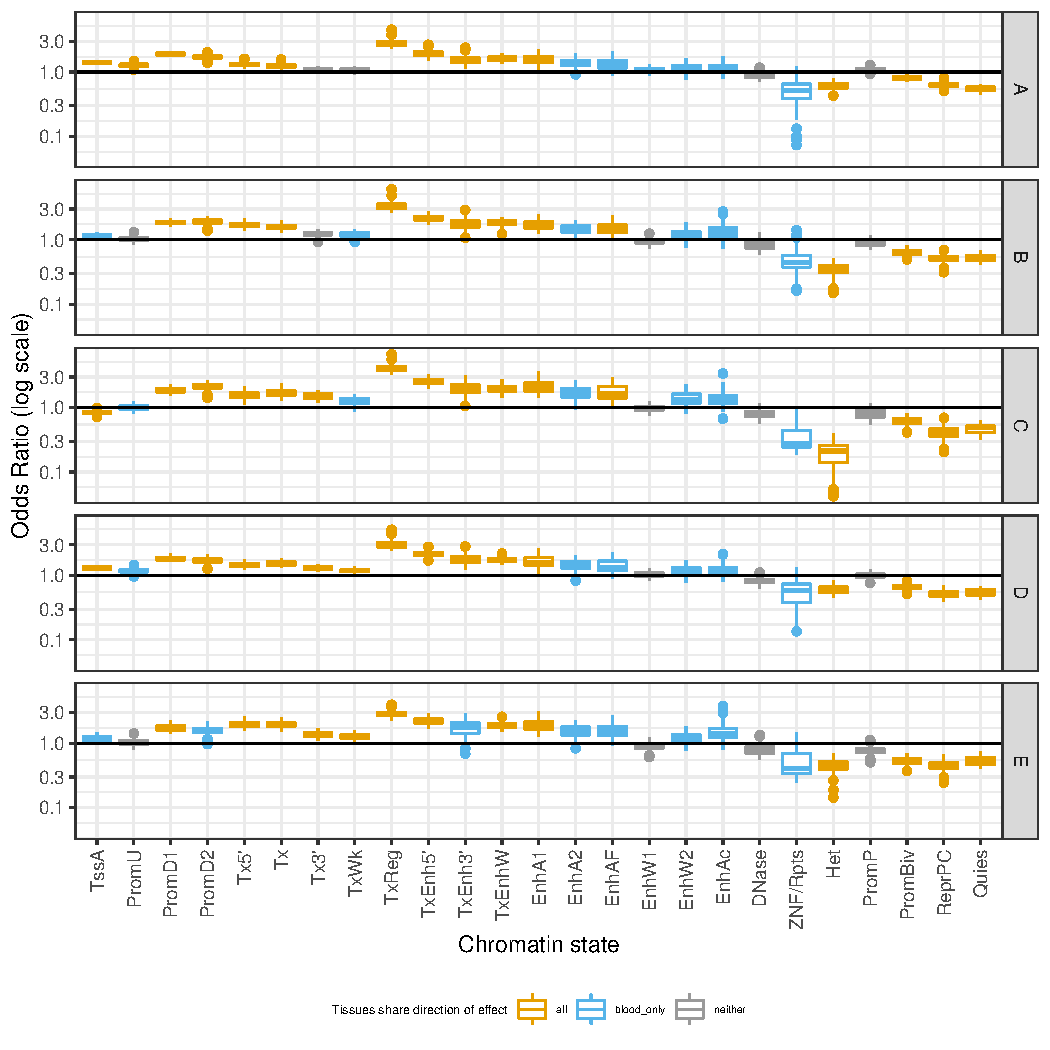
\includegraphics[width=1\linewidth]{figure/04-properties_of_ewas/chromatin_states_enrichment_boxplots_onepage} 

}

\caption[Enrichment of DMPs for 25 chromatin states]{\textbf{Enrichment of DMPs for 25 chromatin states}. Chromatin states across the genome of 127 cell types comprising 25 distinct tissues were available from the Roadmap Epigenomics Project. Using LOLA, the enrichment of DMPs from across all data in The EWAS Catalog for chromatin states were assessed. DMPs were divided into five categories as detailed in \textbf{Section \ref{enrichment-tests-04}}. The x-axis show the 25 chromatin states: TssA, Active TSS; PromU, Promoter Upstream TSS; PromD1, Promoter Downstream TSS with DNase; PromD2, Promoter Downstream TSS; Tx5', Transcription 5'; Tx, Transcription; Tx3', Transcription 3'; TxWk, Weak transcription; TxReg, Transcription Regulatory; TxEnh5', Transcription 5' Enhancer; TxEnh3', Transcription 3' Enhancer; TxEnhW, Transcription Weak Enhancer; EnhA1, Active Enhancer 1; EnhA2, Active Enhancer 2; EnhAF, Active Enhancer Flank; EnhW1, Weak Enhancer 1; EnhW2, Weak Enhancer 2; EnhAc, Enhancer Acetylation Only; DNase, DNase only; ZNF/Rpts, ZNF genes \& repeats; Het, Heterochromatin; PromP, Poised Promoter; PromBiv, Bivalent Promoter; ReprPC, Repressed PolyComb, Quies, Quiescent/Low.}\label{fig:chrom-state-plot}
\end{figure}
The DMPs identified by EWAS were also enriched for transcription factor binding sites. Of the 167 transcription factor binding sites tested, there was evidence that identified DMPs were enriched in 158 of them in at least one tissue type (FDR \textless{} 0.05). The strongest enrichments were found for transcription factor binding sites as measured in blood (median OR ranged from 1.5 to 1.7 based on how DMPs were defined - see \textbf{Section \ref{enrichment-tests-04}} for details) and varied from tissue to tissue, but overall enrichment was observed more often than not across all tissues (\textbf{Figure \ref{fig:tfbs-plot}}).




\begin{figure}

{\centering 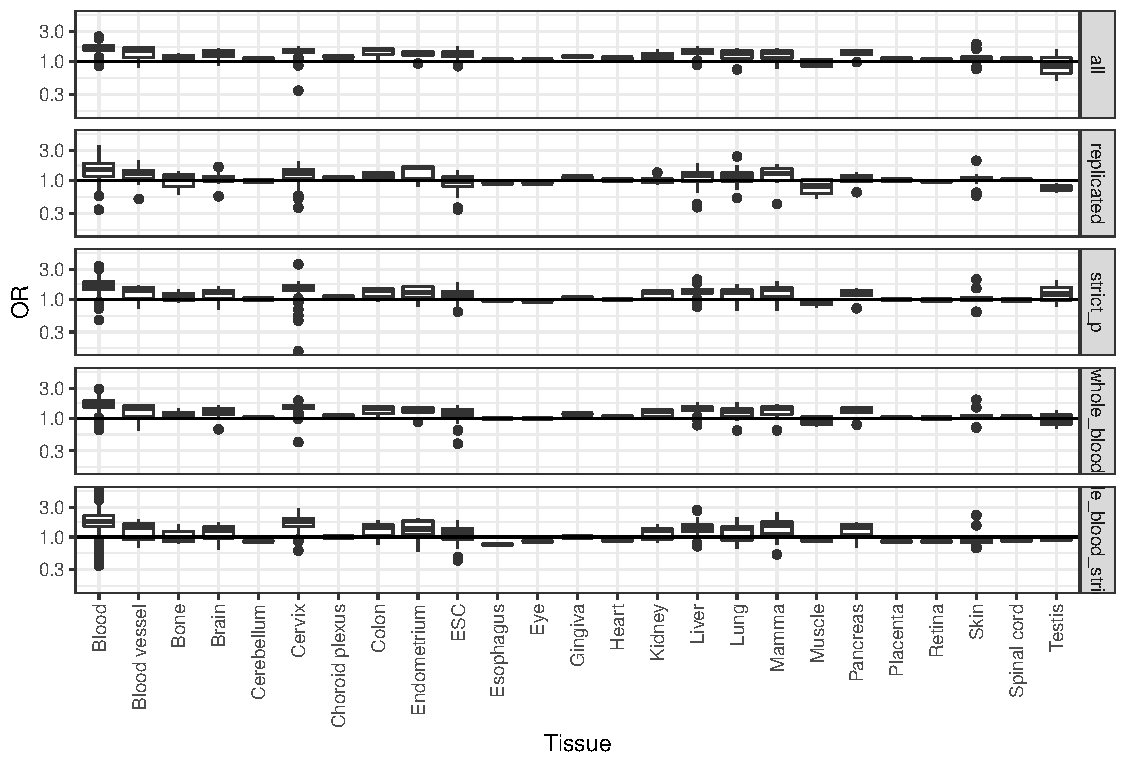
\includegraphics[width=1\linewidth]{figure/04-properties_of_ewas/tfbs_enrichment_plot} 

}

\caption[Enrichment of DMPs for 167 transcription factor binding sites]{\textbf{Enrichment of DMPs for 167 transcription factor binding sites}. Using LOLA, the enrichment of DMPs from across all data in The EWAS Catalog for 167 transcription factor binding sites confirmed across 25 distinct tissues were assessed. DMPs were divided into five categories as detailed in \textbf{Section \ref{enrichment-tests-04}}. The x-axis show the 25 distinct tissues. All transcription factor binding sites have not been confirmed across all tissues. For some tissues (e.g.~``Eye'' and ``Gingiva'') only five have been confirmed, but in blood over 131 have been confirmed.}\label{fig:tfbs-plot}
\end{figure}
\newpage

\hypertarget{discussion-04}{%
\section{Discussion}\label{discussion-04}}

Understanding the nature of EWAS associations is imperative for biological inference. Using data from The EWAS Catalog this chapter shows that many CpGs associate with multiple different unique traits and the magnitude of these associations are partly explained by the characteristics of DNA methylation levels. False positives may also explain a proportion of EWAS associations. Roughly 10\% of the DMPs identified were measured by potentially faulty probes and the median percentage of CpGs that could be replicated across studies was 52\%.

\hypertarget{identifying-mediators}{%
\subsection{Identifying mediators}\label{identifying-mediators}}

Identifying modifiable molecular traits that mediate the effect of complex traits on disease is something that motivates a substantial portion of molecular epidemiology research (49,116). Having a database of associations between DNA methylation and various traits and diseases may enable easy identification of potential mediators that warrant follow-up. Overall, DNA methylation at 126,673 CpGs are associated with multiple traits. The CpG that was identified in the most EWAS, cg06500161 (\emph{ABCG1}), had evidence from multiple studies that methylation at that site associated with weight-related traits such as body mass index (60,70,155,156) and waist circumference (156), roughly 60 metabolites (139,140,157--159) and with type 2 diabetes (160). Some studies have explored these associations further, for example, two studies used Mendelian randomization (MR) to provide evidence that body mass index caused changes in methylation at this site (70,155). However, full characterisation and assessment of whether methylation at that site mediates the effect of adverse adiposity on any diseases has not been undertaken and could be followed-up.

\hypertarget{biased-results}{%
\subsection{Biased results}\label{biased-results}}

The potential biases in EWAS have been well documented (1) and were discussed at length in \textbf{Section \ref{problems-for-ewas}}. It is encouraging that the majority of studies include batch effects and cell composition in at least one of their models (79.1262136\%). However, there are still some studies including probes that have been characterised as faulty.

Differences in cell composition, sample ethnicity, covariates used and other differential biases between studies might explain the low replication rate in some cases. However, studies only tend to report associations below the conventional EWAS P-value threshold, P\textless1x10\textsuperscript{-7}, so differences in study power could also be a major factor.

\hypertarget{understanding-cpg-characteristics}{%
\subsection{Understanding CpG charactersitcs}\label{understanding-cpg-characteristics}}

Characteristics of DNA methylation discovered in experimental studies, such as its association with gene expression, were used to select sites to measure DNA methylation (65). Further, studies have suggested selecting from those sites commonly measured, CpGs that have certain characteristics such as high variance (131,148).

Our results suggest removing CpG sites with low variances may make it more likely to remove sites with greater effects. Variance had a modest ability to predict whether or not a CpG site was likely to be identified in an EWAS, and it did not add to the predictive ability of heritability, despite explaining a higher proportion of variance in effect estimates. This may be explained by two things. Firstly, having a lower variance in the independent or dependent variable increases the standard error of the beta coefficient in a linear regression. Secondly, heritability will in part determine variance of DNA methylation.

\hypertarget{choosing-sites-to-measure}{%
\subsection{Choosing sites to measure}\label{choosing-sites-to-measure}}

As discussed in \textbf{Section \ref{ewas}}, the HM450 array was designed to capture DNA methylation in various regions of the genome. The probes of the array target roughly only 2\% of CpG sites in the genome, yet target over 99\% of protein coding genes and predominantly target the promoter regions of these genes (65). The newer HMEPIC array captures much of what the HM450 does, and further covers 58\% of FANTOM5 enhancers (161).

The trend for DMPs to be enriched for promoter regions (compared to regions of similar CG density) suggests there may have been some justification for the chosen sites. However, not all promoter regions were enriched with DMPs and bivalent promoters were depleted for DMPs. Enrichment of enhancers was also seen, but the magnitude of enrichment was smaller. When designing future arrays, these results suggest that continuing to target promoters and enhancers, whilst avoiding gene regions that are less likely to be actively transcribed may yield more associations in EWAS.

Despite the tissue specific nature of DNA methylation, the regions for which DMPs identified in The EWAS Catalog were found to be enriched were fairly consistent across tissues. However, enrichment of DMPs tended to be greater for blood-based genomic annotations, perhaps reflecting the fact the majority of EWAS in The EWAS Catalog were conducted using DNA methylation measured in whole blood.

\hypertarget{limitations-04}{%
\subsection{Limitations}\label{limitations-04}}

Individual participant data were not available and thus to calculate standardised betas, the variance of the trait had to be estimated from external measures of DNA methylation. If the GoDMC sample is not representative of the sample used for the study EWAS then these estimates may be substantially biased. Further, many studies do not report the effect estimates from their statistical analyses. If there is a marked difference in the studies that do not report effect sizes and those that do, then any associations between standardised effect estimates and DNA methylation site characteristics are likely to be biased.

Like other observable phenotypes, DNA methylation varies under many contexts. Time, sex, tissue type, population, socioeconomic position and many other factors may influence the results of EWAS. The majority of EWAS conducted have used DNA methylation measured in whole blood from European adults making the results not necessarily apply broadly outside those bounds. The need for tissue-specific data has been discussed previously in \textbf{Section \ref{problems-for-ewas}}. Differences in DNA methylation between ethnic groups has been shown previously (162) and the predictive value of a smoking-related methylation score was shown to differ between Europeans and South Asians (143). This suggests any biological insight and population health benefits that may be the result of EWAS is likely to to be maximised by diversifying populations. It is unclear from the work in this chapter whether the CpG characteristics and genomic annotations that show evidence that they influence EWAS results, will also influence EWAS results in the same way within a more ethnically diverse selection of samples.

\hypertarget{conclusion-04}{%
\section{Conclusion}\label{conclusion-04}}

This chapter demonstrates the potential for using large-scale EWAS databases to understand DNA methylation-trait associations. It was found that study design flaws can help explain some associations. However, it is noteworthy that the vast majority of studies have accounted for some potential biasing factors, for example 79\% of studies adjusted for batch effects and cell composition. Further, there was an invese association between DNA methylation variability and effect size, suggesting that studies that remove variable sites prior to analysis could be excluding important regions from the analysis. Finally, cg06500161 \emph{ABCG1} was identified as being associated with 71 traits that share known biological relationships. This highlights the potential to use The EWAS Catalog to identify molecular markers that might underlie the relationship between traits.

\hypertarget{contributions-statement-04}{%
\section{Contributions statement}\label{contributions-statement-04}}

Charlie Hatcher performed the enrichment analyses using LOLA. I visualised the results and did all downstream statistical analyses. As mentioned, I also performed all other analyses and written communication.

\hypertarget{h2ewas-chapter}{%
\chapter{Exploring the variance in complex traits captured by DNA methylation assays}\label{h2ewas-chapter}}

\hypertarget{chapter-summary-05}{%
\section{Chapter summary}\label{chapter-summary-05}}

In \textbf{Chapter \ref{properties-of-ewas}}, various aspects of DNA methylation were shown to correlate with the chances of a CpG site being identified in epigenome-wide association studies (EWAS). However, whether these identified CpG sites, or those that do not associate with with traits at a given P-value threshold, capture much complex trait variance is unclear. Quantifying the total covariation between the DNA methylation marks most commonly measured in EWAS and complex traits, would reveal how much more information is to gain from the current EWAS design if just increasing sample sizes.

In this chapter I estimate the proportion of phenotypic variation captured by 421,693 blood derived DNA methylation markers (h\textsuperscript{2}\textsubscript{EWAS}) across 400 traits. Then I explore whether h\textsuperscript{2}\textsubscript{EWAS} could be used to prioritise traits for which EWAS are likely to yield associations.

I performed all analyses and written communication in this chapter.

\hypertarget{introduction-05}{%
\section{Introduction}\label{introduction-05}}

Epigenome-wide association studies (EWAS) aim to assess the association between phenotypes of interest and DNA methylation across hundreds of thousands of CpG sites throughout the genome (1,66). As seen in \textbf{Chapter \ref{properties-of-ewas}}, many recent EWAS yielded few sites across the genome with strong evidence for association. The proportion of total trait variance associated with each of these sites tended to be small (\textbf{Figure \ref{fig:rsq-distribution}}), but when modelled together, may be large. There is a need to have a global view of the contribution of DNA methylation to complex traits in order to interpret these results.

There are multiple possible reasons for there being few EWAS signals. Firstly, DNA methylation varies between cells and tissues, thus any changes related to a trait may occur in any number of tissues. Currently, because of ease of access and cost, the most common tissue used for EWAS is blood, which may not capture changes in DNA methylation related to the trait of interest (1,66). Secondly, the commonly used technologies probe a small percentage of the total number of potentially methylated sites. In the absence of full knowledge of the correlation structure across methylation site variation, it is therefore difficult to fully understand coverage in current measures. Two more possibilities are that DNA methylation variation is actually not associated with the traits studied or that the associations are many but individually too small to detect with current sample sizes (Box 1).

Interpretation of the paucity of EWAS hits is difficult because there is no knowledge of the total contribution of methylation variation to the trait. However, analogous to the calculation of genetic heritability estimates, which have now been expanded to make inference across non-familial population-level data (SNP heritability), the total contribution of methylation markers to complex traits can potentially be estimated. This could give insight into the underlying patterns of association between DNA methylation markers and complex traits (See Box 2 for a simple explanation of SNP heritability (or h\textsuperscript{2}\textsubscript{SNP}) and its application to DNA methylation).

SNP heritability estimates are sensitive to assumptions of the underlying genetic architecture and there are different ways in which to model the contribution of each SNP to the overall genetic component. The original model of calculating h\textsuperscript{2}\textsubscript{SNP} introduced by Yang et al.~assumes that each variant has an effect that is independent of the regional linkage disequilibrium (LD) structure as each variant is unweighted (the blanket model), and this effectively assumes regions of high LD contribute more to phenotypic variance (99). Speed et al.~proposed a new model, which considered the LD between SNPs so that each region of high LD can effectively be counted as a singular effect (the grouping model) (100). Finding which models fit the data better helps ensure a more accurate estimation of the proportion of DNA methylation association with a trait, further contrasting these models could also be biologically informative.

Gene regions are methylated in a coordinated fashion, which is associated with changes in gene expression (18,163), with a tendency for promotor regions to be unmethylated and gene body regions to be methylated when gene expression is activated (18). This, amongst other complex patterns of gene regulation, induces a correlation structure within EWAS data, and it is not clear whether a single site is driving an association and neighbouring sites are consequentially correlated, or if the cumulative contributions of all neighbouring sites associate with the regulatory process. In EWAS, a common strategy is to collapse DNA methylation sites into groups based on proximity and if they share the same direction of association and potentially magnitude of association, this is often called differentially methylated region (DMR) analysis (164). This, however, does not explain whether the sites within groups are acting independently and cumulatively or as a set of distinct influences. \textbf{Figure \ref{fig:h2ewas-model-comp}} shows a representation of how the differences in models apply to DNA methylation data at a single small region using in one specific example. Of course, there are far more scenarios possible and furthermore, the models aren't restricted to a single small region in the genome. They apply to all sites, as do the DMR methods used in EWAS. Thus, by applying both methods to DNA methylation data across multiple phenotypes and comparing their utility insight can be gained into how DNA methylation operates across gene regions. Furthermore, it is important to find the model that best fits the data to help prevent biased estimates.

This chapter aims to estimate h\textsuperscript{2}\textsubscript{EWAS} values across a plethora of traits and assesses whether this estimate may be useful in identifying traits for which EWAS will likely yield successful identification of associated DNA methylation sites. To do this I perform hundreds of EWAS studies and evaluate if h\textsuperscript{2}\textsubscript{EWAS} estimates are predictive of the number of sites identified by the EWAS at various P value thresholds. I also compare the performance of different models underlying h\textsuperscript{2}\textsubscript{EWAS} estimates to infer likely methylation architecture of complex traits.
\begin{center}\rule{0.5\linewidth}{0.5pt}\end{center}

\textbf{Box 1}

The need for larger sample sizes in GWAS has been empirically demonstrated across a broad range of traits. For height and body mass index (BMI), the number of associations dramatically increased from 12 to 3290 and from one to 941, respectively after increasing sample sizes by \textasciitilde670,000 (165--167). This trend can be seen for many traits. Similar to early GWAS, many EWAS are discovering few sites strongly associated with complex traits. However, an example that suggests promise for increasing sample sizes for EWAS is seen with BMI, where an EWAS of 459 individuals identified just five sites, but increasing the sample size to over 5,000 led to identification of 278 sites (70,168). While we can continue to improve sample sizes in EWAS, there is a need to determine the upper limit of the information we can obtain from EWAS of complex traits like BMI. Furthermore, the BMI EWAS example may be unrepresentative of other traits, so having a corollary test for estimating h\textsuperscript{2}\textsubscript{SNP} for DNA methylation would help us understand if we're capturing relevant information from the current arrays we are using in EWAS. Such information could inform future study designs in terms of growing sample sizes with the current assays available versus designing new assays.
\begin{center}\rule{0.5\linewidth}{0.5pt}\end{center}
\begin{center}\rule{0.5\linewidth}{0.5pt}\end{center}

\textbf{Box 2}

Methods used to estimate h\textsuperscript{2}\textsubscript{SNP} use restricted maximum likelihood (REML) tests to estimate the proportion of variance attributable to these genetic variants. Essentially this assesses whether individuals that are genetically similar are more likely to be phenotypically similar. If those individuals that have a high genetic overlap tend to correlate strongly phenotypically compared to those that don't have high genetic overlap, then the phenotype of interest will have a high h\textsuperscript{2}\textsubscript{SNP}. Unlike genetic variants, DNA methylation is responsive to the environment (1) and determining causal directionality between DNA methylation markers associated with traits is not trivial (49,169,170). Therefore, estimating the proportion of trait variation captured by DNA methylation variation (which will henceforth be denoted as h\textsuperscript{2}\textsubscript{EWAS}) using the same techniques will ascertain effects going in both directions as well as associations due to confounding. The combination of these mechanisms may increase power to detect trait-DNA methylation association, and could be the reason that so many DNA methylation markers are found in small EWAS compared to similarly sized GWAS (70).
\begin{center}\rule{0.5\linewidth}{0.5pt}\end{center}




\begin{figure}

{\centering \includegraphics[width=1\linewidth]{figure/05-h2ewas/m2_model_comparison} 

}

\caption[Comparison of the grouping and blanket models in the context of the relationship between DNA methylation and gene expression]{\textbf{Comparison of the grouping and blanket models in the context of the relationship between DNA methylation and gene expression}. Both regions are exactly the same, the only difference is how each model assumes the methylation sites should be treated. The grouping model down-weights the contribution of correlated CpGs, effectively grouping them, and the blanket model assumes each CpG independently associates with a trait. As seen here, the grouping of correlated CpG sites may not be the correct thing to do as some of the sites may be acting independently of their correlated partners).}\label{fig:h2ewas-model-comp}
\end{figure}
\hypertarget{method-05}{%
\section{Method}\label{method-05}}

\hypertarget{study-samples-05}{%
\subsection{Study samples}\label{study-samples-05}}

All data used in this chapter came from the ARIES subsection of the ALSPAC cohort (see \textbf{Section \ref{aries-02}} for study details). This chapter uses phenotypic and DNA methylation data from 940 mothers at middle age for which data could be extracted. Not all individuals had data on the various covariates used in the analyses, thus the sample size varied with each analysis (mean of 805 and range of 491 to 940).

Continuous and binary phenotypes measured in mothers were extracted from the cohort using the `alspac' R package (github.com/explodecomputer/alspac) and went through extensive quality control. Originally over 15,000 traits that were related to the mothers were extracted from the database. After the quality control process, which is detailed in \textbf{Figure \ref{fig:h2ewas-pheno-qc}}, there were 2408 traits left for analysis.




\begin{figure}

{\centering \includegraphics[width=0.75\linewidth,height=0.75\textheight]{figure/05-h2ewas/m2_data_cleaning} 

}

\caption[A summary of the data cleaning steps]{\textbf{A summary of the data cleaning steps}. Binary variables with fewer than 100 cases or controls were removed. Variables with ``no clear relevance'' to the mothers were identified manually, most were descriptive of how samples were measured, for example the fieldworker that examined the mother several months or years after blood draw. Normality of traits after rank normal transformations were assessed using a Shapiro-Wilk test. Those with some evidence of non-normality (P \textless{} 0.05), were re-examined by eye and removed if thought to be non-normal.}\label{fig:h2ewas-pheno-qc}
\end{figure}
All continuous traits were rank-normalised for further analyses. A Shapiro-Wilk test of normality was performed on these rank-normalised traits and for those with some evidence of non-normality (P \textless{} 0.05), the distribution of those traits was re-examined by eye to ensure it was approximately normal. It was found that any non-normality of phenotype distributions corresponded to an inflation of zero values. These traits were removed and overall there were 2408 traits left for analyses. These traits do not necessarily represent independent phenotypes and as such I wanted to prevent correlated traits skewing results. The absolute Pearson's correlation coefficient between each trait was subtracted from one (1 --{[}r{]}). Then traits were greedily selected where 1 --{[}r{]} \textless{} 0.4 with any other trait. This left 400 traits, which consisted of \textasciitilde30\% clinically measured variables (including roughly 50 metabolites and some anthropometric traits), \textasciitilde25\% health related questions (for example ``have you ever had asthma?''), \textasciitilde40\% behavioural and social traits (for example educational attainment variables, use of pesticide, and having pets), and \textasciitilde5\% of traits were related to the partner or child of the participant (for example the employment status of the partner). Phenotypes are presented in Supplementary table 1. Plots showing the correlation between all the phenotypes as well as with just the selected traits can be seen in \textbf{Figure \ref{fig:h2ewas-pheno-corr-all} and \ref{fig:h2ewas-pheno-corr-subset}}.




\begin{figure}

{\centering \includegraphics[width=1\linewidth]{figure/05-h2ewas/test_correlation_plot_all} 

}

\caption[Correlation between all 2408 phenotypes]{\textbf{Correlation between all 2408 phenotypes}.}\label{fig:h2ewas-pheno-corr-all}
\end{figure}



\begin{figure}

{\centering \includegraphics[width=1\linewidth]{figure/05-h2ewas/test_correlation_plot} 

}

\caption[Correlation between the 400 traits with a correlation of 1 - {[}r{]} \textless{} 0.4]{\textbf{Correlation between the 400 traits with a correlation of 1 - {[}r{]} \textless{} 0.4}.}\label{fig:h2ewas-pheno-corr-subset}
\end{figure}
\hypertarget{dna-methylation-data-05}{%
\subsection{DNA methylation data}\label{dna-methylation-data-05}}

The DNA methylation data also came from ARIES. Measurement, quality control of this data are found in \textbf{Section \ref{aries-dnam-data}}

Probes were excluded if they were present on either of the sex chromosomes, a SNP/control probe, had a detection p value \textless{} 0.05 across over 10\% of samples or were identified as problematic by Zhou et al.~(83). This left 421,693 CpG sites for analyses.

Before analysis a linear regression model was fitted with beta values for methylation (which ranges from 0 (no cytosines methylated) to 1 (all cytosines methylated)) as the outcome against batch variables (plate ID in ALSPAC) modelled as a random effect to help remove the effects of batch in the subsequent analyses.

\hypertarget{reml-analysis}{%
\subsection{REML analysis}\label{reml-analysis}}

Using LDAK (171) the relationship between the methylomes (as measured by the HM450 BeadChip) of 940 individuals was estimated by producing a DNA methylation relationship matrix (MRM). This matrix was used as input for the REML analysis to estimate the proportion of a trait's variation that was explained by DNA methylation (h\textsuperscript{2}\textsubscript{EWAS}). Age, the top 10 ancestry principal components, and derived cell proportions were added as covariates to the model.

When producing the MRM, probes were scaled by their observed variance and the weighting of each probe was based on the variance of DNA methylation at that site using the formula below:
\begin{equation}
    f_{j}(1-f_{j})^{(\alpha/2)}
    \label{eq:mrm-weights}
\end{equation}
where \(f_j(1-f_j)\) is the variance of methylation at CpG \(j\). The higher the alpha value the more weight is given to probes with greater variance; an alpha value of -1 gives equal weight to probes with low and high variance. The alpha value of -0.25 was chosen because previous analysis by Speed et al.~(171) suggested that this value was optimal for measuring h\textsuperscript{2}\textsubscript{SNP}. Furthermore, it was hypothesised that probes with a greater variance would contribute more to trait variance. As the method was applied to DNA methylation data in this chapter, sensitivity analyses were conducted. MRMs were created specifying the alpha value at increasing increments of 0.25 from -2 to 0. The association between h\textsuperscript{2}\textsubscript{EWAS} and number of EWAS hits.

The mean of the MRM diagonal should be 1 and the variance close to 0, as the diagonal values essentially represent the correlation between an individual's methylome with itself. Although values are expected to vary slightly from 1. For the MRMs it was identified that some diagonal elements were very high (\textgreater{} 2), which caused the diagonal to have a high variance (0.13). To assess whether these values could skew results, sensitivity analyses were conducted, removing individuals with varying diagonal value cutoffs.

Like h\textsuperscript{2}\textsubscript{SNP} estimates, h\textsuperscript{2}\textsubscript{EWAS} estimates should range from zero to one. If a trait has a true h\textsuperscript{2}\textsubscript{EWAS} value of zero, there is no association between the methylome and that trait, and if h\textsuperscript{2}\textsubscript{EWAS} equals one then DNA methylation has the capacity to completely predict that trait. However, estimation of h\textsuperscript{2}\textsubscript{EWAS} can be fairly imprecise and without constraining the software it's possible to get estimates of h\textsuperscript{2}\textsubscript{EWAS} that are outside 0-1 due to large standard errors. These point estimates have to be erroneous by definition.

Even though the grouping model effectively groups sites together, it is actually likely to increase the number of parameters because without the weightings imposed by this model, the blanket model essentially ignores sites that are not neighbouring others. Therefore, larger standard errors are expected with the grouping model. The grouping model applies a sliding window approach, with windows of 100kb, to capture the correlation between neighbouring sites and weight sites according to the correlation structure of the region. When applying the grouping model, the number of sites that were weighted were 45,863 (out of 421,693) and the number of sites neighbouring any single CpG site ranged from 29 to 28,217.

\hypertarget{generating-genetic-principal-components}{%
\subsection{Generating genetic principal components}\label{generating-genetic-principal-components}}

Ancestry principal components were generated within ALSPAC mothers using PLINK (v1.9). Before analysis, genetic data went through quality control and were imputed, full details can be found in the Supplementary Material. After quality control and imputation, independent SNPs (r\textsuperscript{2} \textless{} 0.01) were used to calculate the top 10 ancestry principal components.

\hypertarget{methods-ewas-05}{%
\subsection{Epigenome-wide association studies}\label{methods-ewas-05}}

EWAS were conducted for 400 selected traits (see \textbf{Section \ref{study-samples-05}} for selection process) within the ALSPAC cohort. For all traits, linear regression models were fitted with beta values of DNA methylation as the outcome and the phenotype as the exposure. Covariates included age, the top 10 ancestry principal components and cell proportions.

\hypertarget{methods-h2ewas-dmp}{%
\subsection{\texorpdfstring{Association between h\textsuperscript{2}\textsubscript{EWAS} and epigenome-wide association studies results}{Association between h2EWAS and epigenome-wide association studies results}}\label{methods-h2ewas-dmp}}

DMPs were extracted from the EWAS at P value thresholds ranging from 10\textsuperscript{-3} to 10\textsuperscript{-7}. It was assessed whether h\textsuperscript{2}\textsubscript{EWAS} could predict that the number of identified DMPs in an EWAS was greater than number of DMPs expected to be identified at a given P threshold defined as the number of sites tested multiplied by the threshold. The traits were also ``pruned'' in the same way as described above, to prevent including overly correlated traits and biasing results. The sensitivity and specificity of this prediction was calculated and a receiver operating characteristic (ROC) curve was plotted. At p-value thresholds of 10\textsuperscript{-6.5} and 10\textsuperscript{-7} there were than 100 traits for which EWAS identified any sites, so these thresholds were removed from the analysis.

The association between the number of DMPs identified at P \textless{} 1x10\textsuperscript{-5} and h\textsuperscript{2}\textsubscript{EWAS} values was assessed using a negative binomial hurdle model with the number of DMPs identified fitted as the outcome and h\textsuperscript{2}\textsubscript{EWAS} as the exposure. The negative binomial hurdle Poisson regression model results are twofold. The first of which assesses whether there is an association between the binary trait of whether a DMP was identified by EWAS (dependent variable) and h\textsuperscript{2}\textsubscript{EWAS} (independent variable). The second is a zero-truncated model, i.e.~the zero values are removed from the model and the association between number of DMPs (dependent variable) and h\textsuperscript{2}\textsubscript{EWAS} (independent variable) is assessed.

The same method was applied to estimate the association between the number of SNPs identified in GWAS at P \textless{} 5x10\textsuperscript{-8} and h\textsuperscript{2}\textsubscript{SNP}. SNPs associated with 485 traits in UK Biobank (see Supplementary Methods for sample information and phenotype selection) were extracted using the IEU Open GWAS Database (96). The h\textsuperscript{2}\textsubscript{SNP} estimates were extracted from \url{http://www.nealelab.is/uk-biobank/}.

All analyses were conducted in R (version 3.3.3) or using the command line software LDAK (171), GCTA (172), and PLINK (173). For the EWAS analyses, the meffil R package was used (149). A one-sided P value was used to assess if the h\textsuperscript{2}\textsubscript{EWAS} for a trait was \textgreater{} 0, and two-sided P values were used for everything else.

\hypertarget{data-availability-05}{%
\subsection{Data availability}\label{data-availability-05}}

Code used to perform analyses can be found here: github.com/thomasbattram/ereml

The full EWAS summary statistics of each of the 400 EWAS are available via Zenodo here

\hypertarget{results-05}{%
\section{Results}\label{results-05}}

A flowchart showing our study design and giving a summary of the results is shown in \textbf{Figure \ref{fig:h2ewas-study-design}}.




\begin{figure}

{\centering \includegraphics[width=1\linewidth]{figure/05-h2ewas/m2_workflow} 

}

\caption[Study design with a summary of the results]{\textbf{Study design with a summary of the results}. ALSPAC = Avon Longitudinal Study of Parents and Children, QC = quality control, EWAS = epigenome-wide association study, MRM = methylation relationship matrix, AUC = area under curve.}\label{fig:h2ewas-study-design}
\end{figure}
\hypertarget{estimating-h2ewas}{%
\subsection{Estimating the proportion of phenotypic variance associated with DNA methylation}\label{estimating-h2ewas}}

Two models were used to estimate the total contribution of all DNA methylation sites to the variation (h\textsuperscript{2}\textsubscript{EWAS}) for each of 400 traits within up to 940 individuals. The mean for both models was zero with ranges of -0.4 to 0.4 and -0.5 to 0.4 for the blanket and grouping models respectively \textbf{Figure \ref{fig:h2ewas-estimates}}. The estimates were imprecise, the mean standard error was 0.03 and 0.05 for the blanket and grouping models respectively. The trait with the greatest evidence for h\textsuperscript{2}\textsubscript{EWAS} estimates being above zero was having smoked cigarettes regularly (FDR-corrected P = 0.06 and 0.10 for the blanket and grouping models respectively). The correlation between the h\textsuperscript{2}\textsubscript{EWAS} estimates of the two models was 0.47 and there was evidence that on average the estimates of the grouping model were higher (Paired t-test P = 1.8x10\textsuperscript{-5}, \textbf{Figure \ref{fig:h2ewas-estimates}}), and the mean difference between estimates was 0.018.

There was little evidence that either of the models fit the data better (had higher likelihoods) across the 400 traits tested (difference in median likelihoods = 0.19, Wilcoxon's paired ranked sum test P = 0.73). Further, the majority of h\textsuperscript{2}\textsubscript{EWAS} estimate differences between the traits were small.




\begin{figure}

{\centering \includegraphics[width=1\linewidth]{figure/05-h2ewas/model_m2_comparison} 

}

\caption[A comparison of h\textsuperscript{2}\textsubscript{EWAS} estimates given by applying REML using the blanket and grouping models across 400 traits]{\textbf{A comparison of h\textsuperscript{2}\textsubscript{EWAS} estimates given by applying REML using the blanket and grouping models across 400 traits}. The blue dashed line is at x=y. Values with h\textsuperscript{2}\textsubscript{EWAS} lower than 0 are due to imprecision in h\textsuperscript{2}\textsubscript{EWAS} estimates as the true estimate cannot be negative. Smoked\_cigs\_reg = smoked cigarettes regularly. The h\textsuperscript{2}\textsubscript{EWAS} of this phenotype has the greatest evidence for being above 0 for both the blanket and grouping model (Uncorrected P = 1.44x10\textsuperscript{-4} and P = 2.61x10\textsuperscript{-4}, respectively).}\label{fig:h2ewas-estimates}
\end{figure}
\hypertarget{results-sensitivity-analyses-05}{%
\subsection{Sensitivity analyses when estimating the proportion of phenotypic variance associated with DNA methylation}\label{results-sensitivity-analyses-05}}

After examination of the MRMs required to produce the h\textsuperscript{2}\textsubscript{EWAS} estimates, for both the blanket and grouping model some unexpected values were observed. Ninety-six diagonal elements had values over 1.5 when using the blanket model, with the maximum value being 3.562. When assessing the impact of these potential outliers in the MRM to results it was found that the median and range of h\textsuperscript{2}\textsubscript{EWAS} estimates varied little (\textbf{Figure \ref{fig:h2ewas-sens}}). The likelihood of the models tended to be greater as more outliers were removed (lower threshold for classing a diagonal element as an outlier), but it still did not vary greatly (\textbf{Figure \ref{fig:h2ewas-sens}}).

The weight of predictors used to produce the MRMs was also examined. As more weight was given to sites where methylation variation was greater (increasing alpha value) the h\textsuperscript{2}\textsubscript{EWAS} estimates were slightly higher (\textbf{Figure \ref{fig:h2ewas-sens}}). However, the likelihood varied little, the median likelihood had a range of 2 across the alpha values (\textbf{Figure \ref{fig:h2ewas-sens}}).




\begin{figure}

{\centering \includegraphics[width=1\linewidth]{figure/05-h2ewas/sens_boxplots} 

}

\caption[Boxplots summarising of sensitivity analyses]{\textbf{Boxplots summarising of sensitivity analyses}. \textbf{A} and \textbf{B} Analyses estimating h\textsuperscript{2}\textsubscript{EWAS} were repeated after removing individuals who had high diagnonal values in the methylation relationship matrix (MRM). Varying thresholds were used to define individuals as an outlier, NA indicates that no individuals were removed from the analysis. \textbf{A} shows the likelihood estimate (model fit) variation and \textbf{B} shows the variation in h\textsuperscript{2}\textsubscript{EWAS} estimates. Analyses were also repeated in the same vein, varying \(\alpha\) values, (see equation \eqref{eq:mrm-weights}) (\textbf{C} and \textbf{D}).}\label{fig:h2ewas-sens}
\end{figure}
\hypertarget{results-ewas-analyses-05}{%
\subsection{EWAS analyses}\label{results-ewas-analyses-05}}

In order to assess the association between h\textsuperscript{2}\textsubscript{EWAS} and EWAS results, EWAS of 400 traits were performed. No associations were found at the strict P value cutoff of P \textless{} 2.5x10\textsuperscript{-10} (conventional EWAS P-value threshold, 1x10\textsuperscript{-7}, divided by the number of traits, 400). A total of 29 associations between traits and CpGs were identified at the conventional EWAS P value cutoff -- P \textless{} 1x10\textsuperscript{-7}. Of the traits tested, 16 had at least one EWAS hit, with the maximum number of CpGs associated with a trait being 13 (smoked cigarettes regularly). As there were so few traits with any identified hits, I took forward results from the lenient P value threshold of P \textless{} 1x10\textsuperscript{-5}, at which 340 traits had at least one EWAS hit. \textbf{Table \ref{tab:model-testing-tab}} shows each trait and the number of differentially methylated positions identified at varying p-value thresholds.

As the distributions of hit count data was heavily right skewed with an inflation at 0 and 1 (\textbf{Figure \ref{fig:h2ewas-dmp-dist}}), to test the association between h\textsuperscript{2}\textsubscript{EWAS} and number of DMPs I opted to test goodness of fit for variations of Poisson models. Of the 6 models tested, the negative binomial hurdle Poisson regression model fit the data best, full results can be found in Supplementary table 5. It was found there was some evidence for an association between number of EWAS hits and h\textsuperscript{2}\textsubscript{EWAS} (\textbf{Figure \ref{fig:dmps-and-h2ewas}}). There was some evidence of association between the presence of DMPs and h\textsuperscript{2}\textsubscript{EWAS} (beta = 6.2, {[}95\%CI 2.5, 10{]}) as well as some evidence of an association between number of DMPs (when the number is above 0) and h\textsuperscript{2}\textsubscript{EWAS} (mean increase of 0.63, {[}95\%CI 0.41, 0.84{]} DMPs when h\textsuperscript{2}\textsubscript{EWAS} increases by 0.1). Applying the same method to GWAS data, it was found evidence that the presence of identified SNPs associated with h\textsuperscript{2}\textsubscript{SNP} (beta = 21.9 {[}95\%CI 19.6, 24.1{]}) and the association between number of SNPs identified (when the number is above 0) and h\textsuperscript{2}\textsubscript{SNP} (mean increase of 1.5, {[}95\%CI 0.93, 2.5{]} SNPs when h\textsuperscript{2}\textsubscript{SNP} increases by 0.1).




\begin{figure}

{\centering \includegraphics[width=1\linewidth]{figure/05-h2ewas/FOM_hit_count_distribution} 

}

\caption[The distribution of the number of DNA methylation sites identified at P\textless1x10\textsuperscript{-5} across EWAS of 400 traits]{\textbf{The distribution of the number of DNA methylation sites identified at P\textless1x10\textsuperscript{-5} across EWAS of 400 traits}.}\label{fig:h2ewas-dmp-dist}
\end{figure}



\begin{figure}

{\centering \includegraphics[width=1\linewidth]{figure/05-h2ewas/m2_hit_count_scatter_p5_test} 

}

\caption[Association between h\textsuperscript{2}\textsubscript{EWAS} and number of DMPs identified in EWAS]{\textbf{Association between h\textsuperscript{2}\textsubscript{EWAS} and number of DMPs identified in EWAS}. The correlation between DNA methylation and the variance of traits (h\textsuperscript{2}\textsubscript{EWAS}) was calculated using REML analysis using the blanket and grouping models. EWAS were conducted on all the same traits and the distribution of the number of DMPs identified at P \textless{} 1x10\textsuperscript{-5} and h\textsuperscript{2}\textsubscript{EWAS} are plotted above. Any traits where the h\textsuperscript{2}\textsubscript{EWAS} estimate is below 0 are coloured grey. The true h\textsuperscript{2}\textsubscript{EWAS} value of a trait cannot be negative, but sample sizes in this analysis are small so the estimates are imprecise.}\label{fig:dmps-and-h2ewas}
\end{figure}
\begin{table}[!h]

\caption{\label{tab:model-testing-tab}Summary of how well models fit to test the association between $h^2_{EWAS}$ and the number of differentially methylated positions identified across 400 traits at P < 1x10$^{-5}$.}
\centering
\resizebox{\linewidth}{!}{
\begin{tabular}[t]{lrr}
\toprule
Model & Log(likelihood) & DF\\
\midrule
\cellcolor{gray!6}{Poisson} & \cellcolor{gray!6}{-1561} & \cellcolor{gray!6}{2}\\
Negative binomial & -972 & 3\\
\cellcolor{gray!6}{Hurdle-negative binomial} & \cellcolor{gray!6}{-954} & \cellcolor{gray!6}{5}\\
Hurdle & -1500 & 4\\
\cellcolor{gray!6}{Zero-inflated negative binomial} & \cellcolor{gray!6}{-972} & \cellcolor{gray!6}{5}\\
\addlinespace
Zero-inflated Poisson & -1501 & 4\\
\bottomrule
\multicolumn{3}{l}{\textsuperscript{} DF = degrees of freedom.}\\
\end{tabular}}
\end{table}
The ability of h\textsuperscript{2}\textsubscript{EWAS} estimated by both models to predict whether the number of DMPs identified was greater than expected was assessed at varying P value thresholds. ROC curves were produced and the area under the curve (AUC) ranged from 0.65 and 0.67 at P \textless{} 1x10\textsuperscript{-6} to 0.79 and 0.71 at P \textless{} 1x10\textsuperscript{-3} for the blanket and grouping models respectively and the predictive ability remained fairly stable as the threshold increased (\textbf{Figure \ref{fig:h2ewas-dmp-roc-curve}}).




\begin{figure}

{\centering \includegraphics[width=1\linewidth]{figure/05-h2ewas/roc_plot} 

}

\caption[The ability of h\textsuperscript{2}\textsubscript{EWAS} values to predict whether the number of differentially methylated positions identified in an EWAS is higher than expected by chance]{\textbf{The ability of h\textsuperscript{2}\textsubscript{EWAS} values to predict whether the number of differentially methylated positions identified in an EWAS is higher than expected by chance}. ROC curves for h\textsuperscript{2}\textsubscript{EWAS} values predicting number of DMPs at differing P value thresholds. AUC = area under the curve.}\label{fig:h2ewas-dmp-roc-curve}
\end{figure}
\hypertarget{discussion-05}{%
\section{Discussion}\label{discussion-05}}

The global contribution of DNA methylation to complex trait variance can inform researchers of how to design future studies that seek to discover new DNA methylation sites associated with their trait of interest. In this chapter I apply methods designed to estimate the predictive capacity of variants across a SNP-chip (h\textsuperscript{2}\textsubscript{SNP}), to DNA methylation data measured in blood with the HM450 BeadChip across 400 independent traits, giving a distribution of the contribution of all sites typically measured in EWAS to complex trait variance. Although sample size was too small to reliably estimate h\textsuperscript{2}\textsubscript{EWAS} for any one trait, the distribution of estimates suggest little complex trait variation is captured by DNA methylation at the sites measured and h\textsuperscript{2}\textsubscript{EWAS} may be a good measure to identify traits for which EWAS will yield associations.

\hypertarget{estimation-of-h2ewas}{%
\subsection{\texorpdfstring{Estimation of h\textsuperscript{2}\textsubscript{EWAS}}{Estimation of h2EWAS}}\label{estimation-of-h2ewas}}

The true h\textsuperscript{2}\textsubscript{EWAS} of a trait gives the total predictive capacity of DNA methylation for that trait, which is equivalent to the proportion of that trait's total variance that is associated with changes in DNA methylation. Knowing this information can help design future EWAS studies. A low value of h\textsuperscript{2}\textsubscript{EWAS} doesn't necessarily mean there is little correlation between DNA methylation and a trait, it could transpire that unmeasured sites contribute more to the association. It is important to remember that roughly 1.5\% of CpG sites are targeted by the HM450 BeadChip and DNA can be methylated elsewhere (not at cytosine bases). Therefore, whole genome bisulphite sequencing, or a similar technique, may show that the variance of complex traits captured by DNA methylation is far higher. Furthermore, even if h\textsuperscript{2}\textsubscript{EWAS} is low and the sites discovered already do not explain all of the h\textsuperscript{2}\textsubscript{EWAS} estimate, there may still be value in increasing sample size to identify more DMPs as well as increase the precision of h\textsuperscript{2}\textsubscript{EWAS} estimates. DMPs discovered may not be highly correlated with a trait, but this doesn't mean the potential biological information gained isn't valuable. For example, if a change in a the levels of protein X has a large effect on a trait and change in DNA methylation has a small effect on the levels of protein X, then the effect of that DNA methylation change on the trait will be small, but identifying that DMP could lead to discovering the importance of the protein. Another thing to consider is that DNA methylation is tissue and cell specific. This means, that h\textsuperscript{2}\textsubscript{EWAS} may vary a lot depending on what tissue the methylation is measured in.

The true underlying genetic architecture of complex traits is still unknown, and therefore it is difficult to know the appropriate model to choose when estimating the contribution of all measured SNPs to phenotypic variance amongst unrelated individuals and arguments for each model depending on this underlying genetic architecture are still being put forward (171), (174--176), thus the attempts made in this study to re-purpose genomic REML are likely to suffer the same flaws that are trying to be overcome in genetic data. With this in mind, in addition to the imprecise estimates of h\textsuperscript{2}\textsubscript{EWAS} presented here (due to the small sample sizes of available data), we believe that individual trait h\textsuperscript{2}\textsubscript{EWAS} values should be treated with caution. This doesn't exclude the possibility that estimating h\textsuperscript{2}\textsubscript{EWAS} may be useful and other methods are already being developed to measure the association between DNA methylation at all sites and complex traits (177).

\hypertarget{future-ewas-05}{%
\subsection{Future EWAS}\label{future-ewas-05}}

Heritability estimates from family-based studies gave an \emph{a priori} justification for the pursuit of gene mapping endeavours that eventually gave rise to GWAS, as they demonstrated variation in complex traits had a substantial genetic component. However, the evidence DNA methylation contributed to trait variation was not ascertained before EWAS were first conducted. To justify collecting more samples and continuing with EWAS research in the current vein, methods such as the one presented in this study should be used to show DNA methylation does substantially contribute to trait variance.

It has become clear from the GWAS era of genetics, that for complex traits, such as coronary artery disease, many common genetic variants with small effects make up the genetic component of the trait (178,179). This suggests a large number of molecular pathways contribute to these traits. DNA methylation at CpGs is heritable (3,151), thus it would be expected that the DNA methylation architecture of a trait will somewhat reflect the genetic architecture of the trait, although this has not been empirically tested.

Despite uncertainty of h\textsuperscript{2}\textsubscript{EWAS} estimates for individual traits, I show h\textsuperscript{2}\textsubscript{EWAS} has a modest ability to predict whether the number of EWAS hits will be greater than expected by chance at a given P value threshold. This predictive ability remained stable as the P value threshold for detection increased from P \textless{} 1x10\textsuperscript{-6} to P \textless{} 1x10\textsuperscript{-3}. These results suggest that increasing sample sizes for traits which truly associate with DNA methylation should result in the discovery of more DMPs. Furthermore, these results support a model for which small changes in methylation at many CpGs across the genome are related to complex traits.

\hypertarget{contribution-of-individual-cpg-sites}{%
\subsection{Contributions of individual CpG sites}\label{contribution-of-individual-cpg-sites}}

The original model for measuring h\textsuperscript{2}\textsubscript{SNP} assumed all genetic variants contributed the same effect on a trait (99), Speed et al.~offered an alternative model assuming a different underlying genetic architecture, whereby genetic variants in regions of high LD contributed less to the variance of a trait than more independent variants. Both groups have shown that the performance of the models depend on the alignment of the trait's architecture with the models' underlying assumptions. Previous literature has suggested that it is the methylation across groups of CpGs that may affect how other molecules interact with DNA and influence cellular functions such as gene expression (18). Furthermore, CpGs are not randomly distributed throughout the genome -- many exist in close proximity within ``islands'' or other regions, suggesting that grouping of the CpGs may have functionality. However, the most common method used in EWAS is to treat CpG sites as independent. Here, the models proposed by Speed et al.~(the grouping model) and Yang et al.~(the blanket model), when estimating h\textsuperscript{2}\textsubscript{EWAS} were tested across 400 traits. The model fit the data better (had a higher likelihood) 207 times for the blanket model and 193 times for the grouping model. Thus for over half the traits treating DNA methylation sites as independent seems to be preferable and even though there is correlation between CpG sites, which allows them to be grouped, it might be that in some groups of correlated sites, individual sites within the group contribute separately to trait variance.

It's important to note that the grouping method takes into account correlation between CpGs within 100Kb of each other. Differential methylation at CpG sites may be correlated for a variety of biological reasons, for example, CpGs lying within a transcription factor binding site will be regulated together, but also, they will be correlated with CpGs that lie in other binding sites for that same transcription factor and these may be many megabases away. This is relevant to the relationship between DNA methylation and complex traits because transcription factor regulation might be the link between complex traits and DNA methylation. Even though grouping CpG sites might yet be the best way to model the relationship between DNA methylation and complex traits, the optimum way to group sites is unknown and will likely change depending on the trait of interest.

\hypertarget{limitations-05}{%
\subsection{Limitations}\label{limitations-05}}

The main limitation of the chapter is the small sample size (maximum N = 940) to estimate the h\textsuperscript{2}\textsubscript{EWAS}. This meant the precision of our h\textsuperscript{2}\textsubscript{EWAS} estimates were very low and so our power to assess their ability to predict number of DMPs and find individual trait h\textsuperscript{2}\textsubscript{EWAS} values was low. To circumvent this problem, trends across multiple traits are assessed and I do not make strong conclusions for any one trait.

As mentioned previously the HM450 BeadChip captures a small percentage of the total DNA methylome and h\textsuperscript{2}\textsubscript{EWAS} estimates will likely vary upon assaying more DNA methylation sites. Furthermore, when measuring more sites, it might be that one of the models fits the data better. Nevertheless, the results of this study can still give evidence towards the hypothesis that differential methylation at many sites across the genome each contribute minimally to the overall association between the methylome and a complex trait.

Unlike germline genetic variants, there is intra-individual (between tissue and time dependent) DNA methylation variation (1,66). Thus, it is to be expected that the variation of h\textsuperscript{2}\textsubscript{EWAS} estimates across traits is partly a product of the tissue and timepoint of choice. However, within the tissue biologically pertinent to the complex trait of interest, the number of pathways that associate with variation in that trait is likely to remain high, for example there are many processes affecting, or affected by, cancer development (180). Thus, it would still be expected that differential methylation at many CpG sites each associate with a trait, but the effect sizes are small. The same can be said when estimating h\textsuperscript{2}\textsubscript{EWAS} at various timepoints.

Estimates of h\textsuperscript{2}\textsubscript{EWAS} will be a product of their environment and genetic makeup of the participants it's measured in. Therefore, the results here may vary by population and by sex. However, participants used in this study are considered to be representative of the larger ALSPAC cohort (181), which is itself considered to be representative of a large majority of women from the UK and potentially other high-income countries (126). This suggests the results will be generalisable to a large group of samples for which EWAS are conducted, but replication in these samples as well as in different populations would provide greater confidence in the generalisability of the results.

A wide range of complex traits was used in the analysis, but there are some notable absences. Rarer diseases and diseases that predominantly impact the elderly are not present in this study. The results presented here cannot be generalised to those traits.

The factors important for the correlation structure of DNA methylation data are less known than those for linkage disequilibrium structure of genetic variants. Therefore, when applying models, such as the grouping model here, that aim to account for correlation of neighbouring DNA methylation sites, some of the important structure captured may be missed for example by trans-correlations (over 1Mb). A model that estimates h\textsuperscript{2}\textsubscript{EWAS} by incorporating all of the underlying correlation of DNA methylation data may therefore outperform both models tested here.

\hypertarget{conclusion-05}{%
\section{Conclusion}\label{conclusion-05}}

Overall, the number of traits with good evidence for h\textsuperscript{2}\textsubscript{EWAS} \textgreater{} 0 was low (only smoking behaviour met the threshold of FDR \textless{} 0.1) and mean h\textsuperscript{2}\textsubscript{EWAS} value across both models was roughly 0, suggesting that for many traits DNA methylation variation as measured on the HM450 BeadChip in blood is of little relevance. However, these estimates varied greatly and therefore DNA methylation measured in this way will likely have relevance for some traits, for example smoking cigarettes regularly. Further, these estimates were correlated with the number of DMPs identified, suggesting that for traits whose variance associates with DNA methylation then increasing sample size will yield an increase in the number of CpGs identified in EWAS. I also provide evidence that there is value in assessing individual CpG-trait associations as opposed to groups of correlated CpG sites within 100Kb. However, this does not preclude the possibility that a more complex model of CpG site correlation may provide a better fit.

\hypertarget{ewas-gwas-comp-chapter}{%
\chapter{A comparison of the genes and genesets identified by EWAS and GWAS of eight complex traits}\label{ewas-gwas-comp-chapter}}

\hypertarget{chapter-summary-06}{%
\section{Chapter summary}\label{chapter-summary-06}}

Despite little evidence that DNA methylation correlates highly with complex trait variation (\textbf{Chapter \ref{h2ewas-chapter}}), it is of interest to understand whether the DNA methylation sites identified may be valuable in understanding the underlying biology of complex traits. As discussed previously, it is well understood that observational associations between DNA methylation and complex traits are sucesptible to confounding and reverse causation. Genetic variants identified in GWAS will not be caused by phenotypic variation and their associations with complex traits are unlikely to be confounded. Yet, both GWAS and EWAS aim to identify regions of the genome that will give an indication of the molecular nature of complex traits.

Using data from The EWAS Catalog (\textbf{Chapter \ref{ewas-catalog}}) and the IEU OpenGWAS Project (95,96), in this chapter I examine whether EWAS is likely uncovering similar facets of complex trait aeitiology to GWAS.

I conducted all analyses and did the written communication in this chapter.

\hypertarget{introduction-06}{%
\section{Introduction}\label{introduction-06}}

Often in EWAS, the potential biological implications of differentially methylated positions or regions (DMPs or DMRs) will be investigated further through genomic annotations (182--185). As discussed in \textbf{Section \ref{dna-methylation}}, previous studies have demonstrated a relationship between DNA methylation levels and proximal genes (18,32). This observation has lead to it being common place to map sites identified in EWAS to nearby genes and these genes and their function are often probed to ascertain their relevance to the trait of interest (182--185). Further, genes can be grouped with others into ``genesets'' that have similar functionality or lie within the same pathway. Over-represented genesets may provide an insight into the molecular biology of a trait, for example, DNA methylation sites identified in an autoimmune disease EWAS might tag genes within immunological pathways more than expected by chance. Other assessments may be made to infer potential biological understanding, including enrichment of other epigenetic marks at the regions identified (186) and follow-up experimental studies (66). However, using open access databases to investigate tagged genes and genesets is a simple and potentially effective approach to further biological understanding.

GWAS often use similar approaches to EWAS to help infer function from the signals identified (66,187). However, the properties of genetic variants and DNA methylation differ making potential inferences from EWAS and GWAS diverge. Importantly, DNA methylation is responsive to environmental stimuli, thus making associations identified in EWAS potentially attributable to reverse causation and to confounding (1,49,181). It should be noted GWAS may be susceptible to confounding, but it is reasonable to assume it is less pervasive amongst GWAS associaitons (92,93).

Given what is known about the properties of genetic variants, a direct comparison between EWAS and GWAS results can provide insight into what biological information EWAS is capturing. If EWAS are highlighting a similar set of genes and genesets, it suggests changes in DNA methylation are identifying facets of trait aetiology. In the event that GWAS and EWAS are not highlighting similar genes and genesets, it is plausible that EWAS may still be identifying facets of trait aetiology. If DNA methylation mediates non-genetic effects and if sites are mapped to genes or genesets incorrectly then overlap will not be guarenteed even if DNA methylation identified is aetiologically relevant. When DNA methylation mediates the effect of genetic variants distal to their genomic position on complex traits, the genes identified by GWAS and EWAS will also differ, but the genesets would likely overlap. The lack of overlap could also reflect the fact associations in EWAS may be driven by confounding and reverse causation. Despite the caveats mentioned, one might still expect to detect overlap in genes and genesets identified by EWAS and GWAS of corresponding traits in the absence of confounding and reverse causation. The extent to which this expectation holds is discussed in more detail in the \textbf{Section \ref{discussion-06}}.

In this chapter, the overlap between genes and genesets identified by GWAS and EWAS of eight complex traits is explored and the scenarios in which one would and would not expect to find overlap are modelled through simulations.

\hypertarget{results-06}{%
\section{Results}\label{results-06}}

\hypertarget{study-data}{%
\subsection{Study data}\label{study-data}}

Traits were selected for which EWAS had been conducted with over 4500 samples and for which corresponding GWAS summary data were available. At the time of conducting these analyses, traits were identified using data from The EWAS Catalog (\textbf{Chapter \ref{ewas-catalog}}) that contained EWAS published before 2019. The EWAS of glucose and insulin were also added at a later date. Traits and study data information is in \textbf{Table \ref{tab:trait-data-tab-06}}.
\begin{table}[!h]

\caption{\label{tab:trait-data-tab-06}Study data}
\centering
\resizebox{\linewidth}{!}{
\begin{tabular}[t]{lllllll}
\toprule
trait & ewas-author & ewas-pmid & ewas-n & gwas-author & gwas-pmid & gwas-n\\
\midrule
\cellcolor{gray!6}{current versus never smoking} & \cellcolor{gray!6}{Joehanes R} & \cellcolor{gray!6}{27651444} & \cellcolor{gray!6}{9,389} & \cellcolor{gray!6}{Liu M} & \cellcolor{gray!6}{30643251} & \cellcolor{gray!6}{632,802}\\
former versus never smoking & Joehanes R & 27651444 & 13,474 & Elsworth B & NA & 424,960\\
\cellcolor{gray!6}{alcohol consumption per day} & \cellcolor{gray!6}{Liu C} & \cellcolor{gray!6}{27843151} & \cellcolor{gray!6}{9,643} & \cellcolor{gray!6}{Liu M} & \cellcolor{gray!6}{30643251} & \cellcolor{gray!6}{537,349}\\
c-reactive protein & Ligthart S & 27955697 & 8,863 & Ligthart S & 30388399 & 204,402\\
\cellcolor{gray!6}{body mass index} & \cellcolor{gray!6}{Wahl S} & \cellcolor{gray!6}{28002404} & \cellcolor{gray!6}{10,238} & \cellcolor{gray!6}{Yengo L} & \cellcolor{gray!6}{30124842} & \cellcolor{gray!6}{681,275}\\
\addlinespace
educational attainment & Karlsson Linner R & 29086770 & 10,767 & Lee JJ & 30038396 & 766,345\\
\cellcolor{gray!6}{insulin} & \cellcolor{gray!6}{Liu J} & \cellcolor{gray!6}{31197173} & \cellcolor{gray!6}{4,740} & \cellcolor{gray!6}{Manning AK} & \cellcolor{gray!6}{22581228} & \cellcolor{gray!6}{51,750}\\
glucose & Liu J & 31197173 & 4,808 & Manning AK & 22581228 & 58,074\\
\bottomrule
\multicolumn{7}{l}{\textsuperscript{} Where gwas-pmid = NA, the GWAS were conducted as part of a UK Biobank GWAS pipeline within the}\\
\multicolumn{7}{l}{Univeristy of Bristol's Integrative Epidemiology Unit and can be found on the OpenGWAS Project website}\\
\multicolumn{7}{l}{(see Methods for more)}\\
\end{tabular}}
\end{table}
\hypertarget{genomic-position-overlap}{%
\subsection{Genomic position overlap}\label{genomic-position-overlap}}

The genome was divided into 5591 500kb non-overlapping regions and mapped EWAS and GWAS signals for each trait to these regions (see \textbf{Section \ref{methods-06}} for more details). The number of regions that were identified by one study type and not the other was higher for each trait than the number of overlapping regions (\textbf{Figure \ref{fig:overlap-barplot}}). Further, the magnitude of the greatest GWAS effect estimate in each region had little ability to predict whether or not a DNA methylation site was likely to be identified in the same region (AUC range = 0.43-0.56, \textbf{Figure \ref{fig:auc-plot}}).




\begin{figure}

{\centering 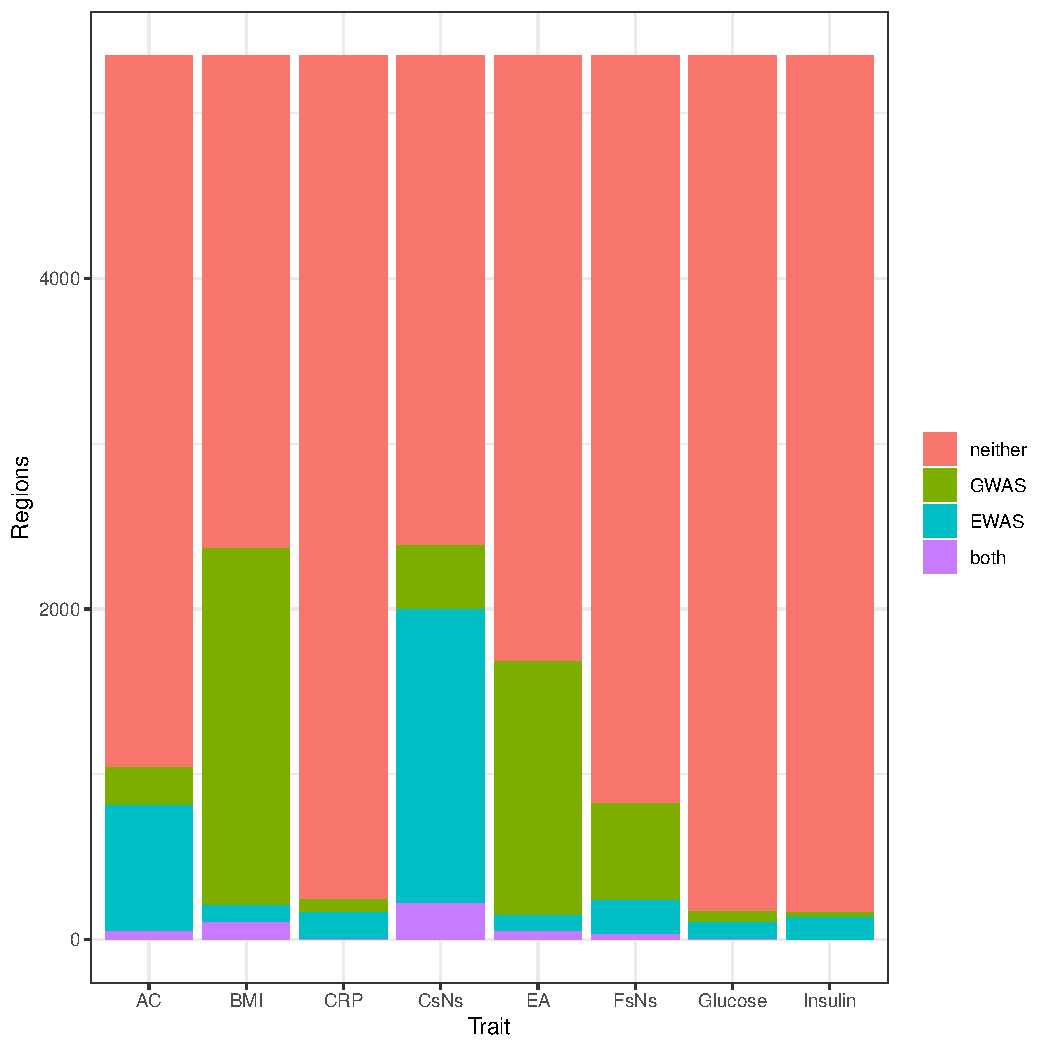
\includegraphics[width=1\linewidth]{figure/06-ewas_gwas_comparison/all_traits_overlap_bar} 

}

\caption[Overlap between genomic positions identified by corresponding EWAS and GWAS]{\textbf{Overlap between genomic positions identified by corresponding EWAS and GWAS}. The genome was divided into 500Kb regions. Those where no probes on the HM450 array measured DNA methylation were excluded from the analysis. Regions were counted as being identified by a GWAS if one or more SNPs associated with the trait and as being identified by an EWAS if one or more CpGs associated with the trait. Neither = no EWAS or GWAS sites identified in the region, GWAS = GWAS sites only were identified, EWAS = EWAS sites only were identified, Both = Both EWAS and GWAS sites were identified, AC = alcohol consumption per day, BMI = body mass index, CRP = c-reactive protein, CsNs = current smokers vs never smokers, EA = educational attainment, FsNs = former smokers vs never smokers.}\label{fig:overlap-barplot}
\end{figure}



\begin{figure}

{\centering 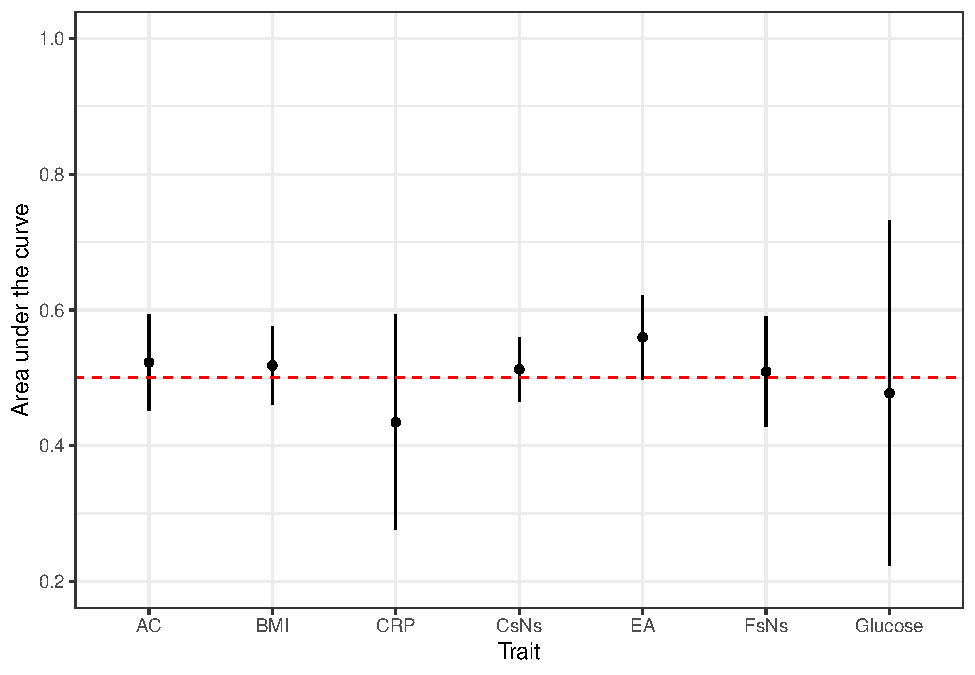
\includegraphics[width=1\linewidth]{thesis_files/figure-latex/auc-plot-1} 

}

\caption[Can genetic variant associations predict the presence of DNA methylation associations in the same region?]{\textbf{Can genetic variant associations predict the presence of DNA methylation associations in the same region?.} For each 500kb region in the genome, the largest SNP-trait effect size was extracted. ROC curves were produced to determine whether these could predict whether a differentially methylated position related to the same trait was present in the same 500kb region. The area under these curves (AUC), with their confidence intervals, are plotted for each trait. The red dashed line is at AUC = 0.5, which represents a prediction no better than chance. AC = alcohol consumption per day, BMI = body mass index, CRP = c-reactive protein, CsNs = current smokers vs never smokers, EA = educational attainment, FsNs = former smokers vs never smokers. Note: insulin is not present in this plot as there were GWAS and EWAS signal that overlapped across all the 500kb regions.}\label{fig:auc-plot}
\end{figure}
\hypertarget{assessing-power-sims}{%
\subsection{Assessing power to detect shared annotations between GWAS and EWAS}\label{assessing-power-sims}}

Genomic function and trait biology are not divided into discrete 500kb genomic chunks, thus GWAS and EWAS could still be identifying similar facets of trait biology without identifying the same genomic regions.

I sought to assess whether the genes and genesets identified overlapped more than expected by chance, thus genomic positions were mapped to genes and genes to genesets (details in \textbf{Section \ref{methods-06}}). Overlap between genes identified was assessed using Fisher's exact test. Two methods for testing overlap between genesets were considered, one simply mapped genes to genesets and used Fisher's exact test in the same way as assessing overlap between identified genes. The other generated `enrichment scores' for each geneset and assessed correlation between the geneset enrichment scores across studies.

Assuming all genetic effects on DNA methylation are proximal. If all DMPs that associated with a trait were on the pathway from SNP to disease, then EWAS and GWAS would be identifying genes from the exact same geneset (i.e.~genes that caused changes in the trait). The more DMPs that are identified because of confounding effects or reverse causation, the smaller the chance of overlap, assuming that causal and responsive genesets are distinct. As mentioned, the presence of trans-mQTLs would make the overlap of genes identified by GWAS and EWAS less likely despite both studies identifying aetiologically relevant factors. However, geneset overlap will be more likely to be maintained regardless of trans-mQTL presence. In a scenario where no DMPs are causing phenotypic changes, any overlap in genes and genesets found would be entirely attributable to chance (ignoring potential feedback loops whereby the trait causes changes in genesets that it is affected by). Simulations were run to assess which scenarios the enrichment and annotation methods had power to detect whether there was more overlap than expected by chance. Power was also assessed across different annotation methods. A schematic of how the simulations were set up can be found in \textbf{Figure \ref{fig:method-simulations-schematic}}.




\begin{figure}

{\centering 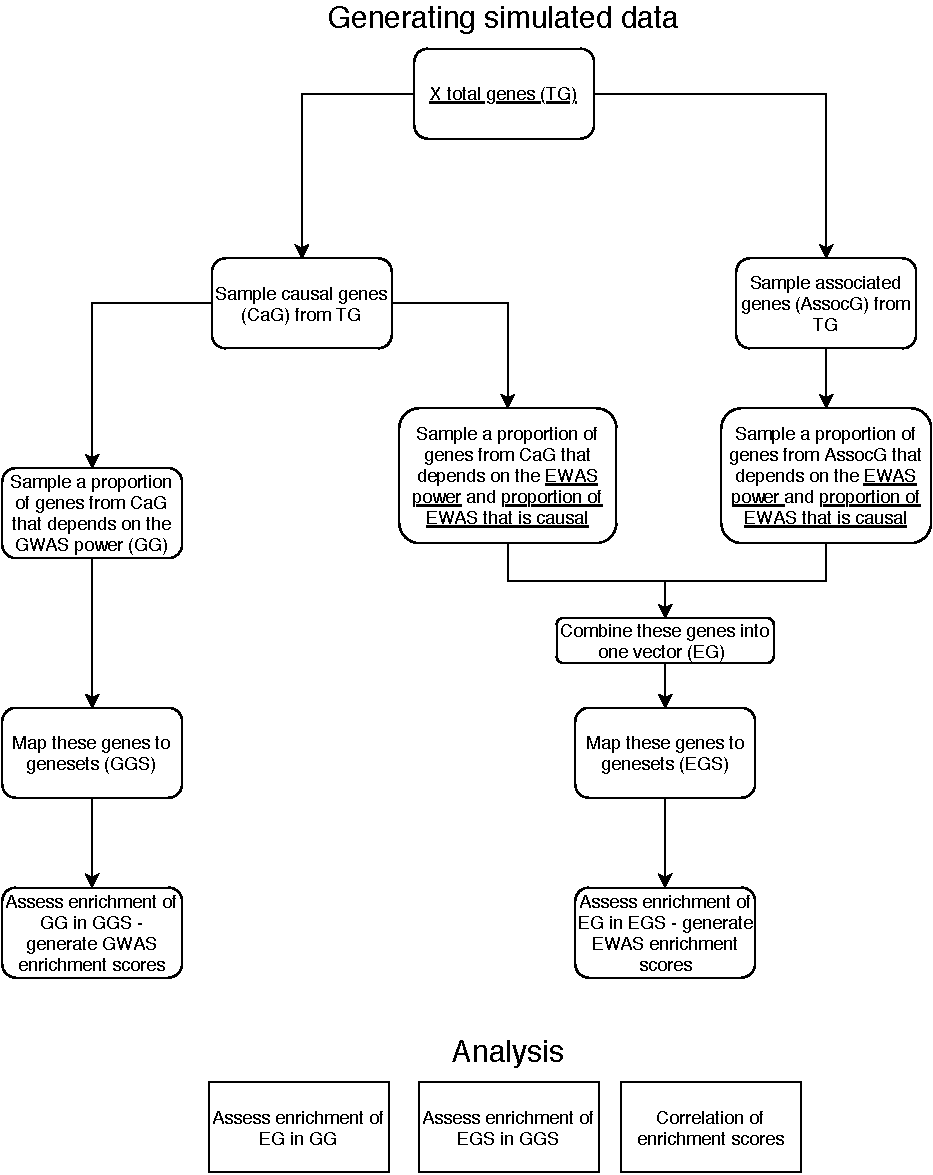
\includegraphics[width=1\linewidth]{figure/06-ewas_gwas_comparison/simulations-gene-up-flowchart} 

}

\caption[Flowchart demonstrating how the first set of simulations were set up]{\textbf{Flowchart demonstrating how the first set of simulations were set up}. The flowchart (under the title ``Generating simulated data'') shows how the simulated data were generated. The boxes under ``Analysis'' show the analyses performed with the simulated data. Underlined parameters were varied. The simulations were repeated 1000 times for each set of parameters.}\label{fig:method-simulations-schematic}
\end{figure}
Under each scenario, the ability to predict whether EWAS were identifying, in part, the same set of genes as GWAS (`causal genes') compared to a random set of genes (`associated genes') was tested. As expected, predictive capacity increased as study power and the proportion of causal DMPs increased (\textbf{Figure \ref{fig:sim1-summ-plot}}, \textbf{Figure \ref{fig:sim1-full-plot5}}). Predictive ability tended to increase as the number of identified genes increased, but this parameter was largely inconsequential when the proportion of causal DMPs was low (\textbf{Figure \ref{fig:sim1-full-plot5}}). Performance was similar across annotation methods and between methods attempting to assess geneset overlap, with assessment of gene overlap performing better (\textbf{Figure \ref{fig:sim1-summ-plot}}). Overall there was more power to detect overlap in genes than overlap in genesets. Between the geneset methods, there was more power to detect correlation between enrichment scores than direct overlap in genesets. Therefore, gene overlap and correlation between geneset enrichment scores were taken forward for the empirical analyses. Assessing correlations of GO term genesets had slightly more power (\textbf{Figure \ref{fig:sim1-summ-plot}}) than other geneset databases, so these geneset annotations were taken forward.




\begin{figure}

{\centering 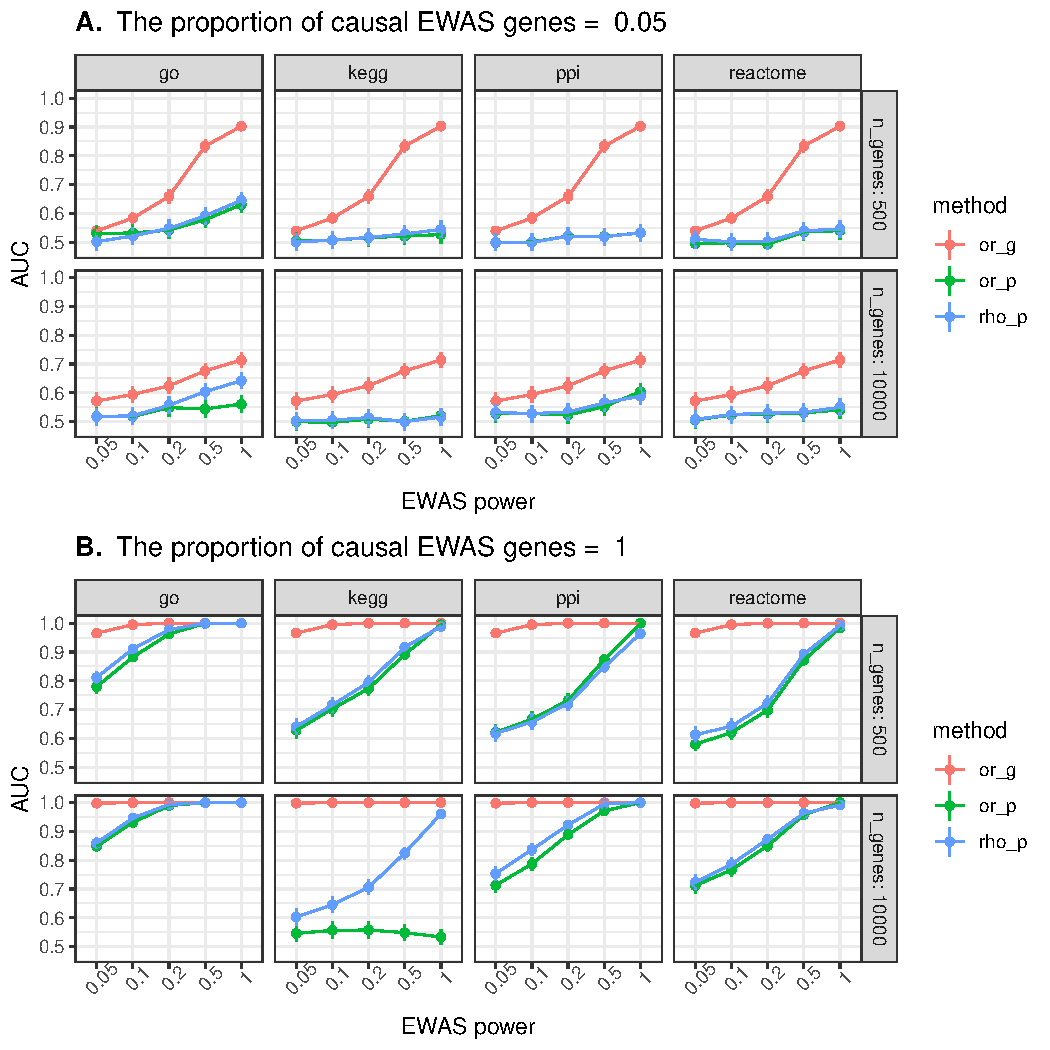
\includegraphics[width=1\linewidth]{figure/06-ewas_gwas_comparison/methods_test_gene_up_auc_plot_all_databases_summary} 

}

\caption[Power to detect overlap between genes and genesets identified by corresponding EWAS and GWAS]{\textbf{Power to detect overlap between genes and genesets identified by corresponding EWAS and GWAS.} Simulations were set up as illustrated in \textbf{Figure \ref{fig:method-simulations-schematic}}. The area under receiver operator curves (AUC) was used to estimate the ability to distinguish between results generated when EWAS and GWAS were sampling, in part, from the same set of causal genes and results generated when EWAS were sampling random genes from the genome. The header of each set indicates the proportion of genes identified by the simulated EWAS that were set to be causal. or\_g = assessing overlap of genes, or\_p = assessing overlap of genesets, rho\_p = assessing correlation between geneset enrichment scores. go = gene ontology, ppi = protein-protein interaction database from EpiGraphDB. This is a summary of the results, full results can be found in \textbf{Figure \ref{fig:sim1-full-plot5}}.}\label{fig:sim1-summ-plot}
\end{figure}
\hypertarget{gwas-ewas-overlap}{%
\subsection{Gene and geneset overlap between GWAS and EWAS}\label{gwas-ewas-overlap}}

For the eight traits used, the number of genes identified by EWAS and GWAS that overlapped was low and for two traits no genes identified by the studies overlapped (\textbf{Table \ref{tab:empirical-gene-tab}}). The number of genesets that overlapped was higher, peaking at 1,243 for GWAS and EWAS of body mass index (\textbf{Table \ref{tab:empirical-pathway-tab}}).

There was no strong evidence that the number of overlapping genes identified was more than expected by chance (\textbf{Table \ref{tab:empirical-gene-tab}}). Although, power was low in most cases to detect a high level of gene overlap in most cases. There was also little evidence that correlation between enrichment scores of the GO terms was greater than expected by chance (\textbf{Table \ref{tab:empirical-pathway-tab}}). As suggested by the previous simulations, this does not preclude the possibility that EWAS are identifying changes in DNA methylation that are upstream of phenotypic change. \linebreak
\begin{table}[!h]

\caption{\label{tab:empirical-gene-tab}Overlap of genes identified by EWAS and GWAS}
\centering
\resizebox{\linewidth}{!}{
\begin{tabular}[t]{llllllll}
\toprule
trait & n-ewas-genes & n-gwas-genes & gene-overlap & obs-OR & exp-gene-overlap & exp-OR & p-diff\\
\midrule
\cellcolor{gray!6}{current versus never smoking} & \cellcolor{gray!6}{1,933} & \cellcolor{gray!6}{312} & \cellcolor{gray!6}{27} & \cellcolor{gray!6}{2.9} & \cellcolor{gray!6}{39} & \cellcolor{gray!6}{3.42} & \cellcolor{gray!6}{0.322}\\
former versus never smoking & 282 & 320 & 9 & 6.4 & 7 & 3.43 & 0.022\\
\cellcolor{gray!6}{alcohol consumption per day} & \cellcolor{gray!6}{361} & \cellcolor{gray!6}{196} & \cellcolor{gray!6}{3} & \cellcolor{gray!6}{2.6} & \cellcolor{gray!6}{3} & \cellcolor{gray!6}{2.44} & \cellcolor{gray!6}{0.908}\\
c-reactive protein & 189 & 302 & 3 & 3.2 & 1 & 0.91 & 0.121\\
\cellcolor{gray!6}{body mass index} & \cellcolor{gray!6}{232} & \cellcolor{gray!6}{3,221} & \cellcolor{gray!6}{23} & \cellcolor{gray!6}{2.0} & \cellcolor{gray!6}{39} & \cellcolor{gray!6}{3.04} & \cellcolor{gray!6}{0.052}\\
\addlinespace
educational attainment & 25 & 1,594 & 1 & 1.5 & 3 & 3.00 & 0.430\\
\cellcolor{gray!6}{insulin} & \cellcolor{gray!6}{36} & \cellcolor{gray!6}{5} & \cellcolor{gray!6}{0} & \cellcolor{gray!6}{0.0} & \cellcolor{gray!6}{0} & \cellcolor{gray!6}{0.00} & \cellcolor{gray!6}{1.000}\\
glucose & 15 & 50 & 0 & 0.0 & 0 & 0.00 & 1.000\\
\bottomrule
\multicolumn{8}{l}{\textsuperscript{} exp = expected, obs = observed}\\
\multicolumn{8}{l}{\textsuperscript{} odds ratios (ORs) can be interpreted as the odds of an gene being identified by EWAS and a GWAS over the odds}\\
\multicolumn{8}{l}{of a gene being identified by an EWAS but not by a GWAS.}\\
\multicolumn{8}{l}{\textsuperscript{} exp-OR = the mean OR after repeating the analysis 1000 times, randomly sampling EWAS genes equal to the}\\
\multicolumn{8}{l}{number identified in the empirical analysis.}\\
\end{tabular}}
\end{table}
\begin{table}[!h]

\caption{\label{tab:empirical-pathway-tab}Correlation of geneset enrichment scores between EWAS and GWAS}
\centering
\resizebox{\linewidth}{!}{
\begin{tabular}[t]{lllllll}
\toprule
trait & n-ewas-genes & n-gwas-genes & geneset-overlap & obs-cor & exp-cor & p-diff\\
\midrule
\cellcolor{gray!6}{current versus never smoking} & \cellcolor{gray!6}{1,933} & \cellcolor{gray!6}{312} & \cellcolor{gray!6}{1,053} & \cellcolor{gray!6}{0.200} & \cellcolor{gray!6}{0.22} & \cellcolor{gray!6}{0.034}\\
former versus never smoking & 282 & 320 & 661 & 0.298 & 0.30 & 0.994\\
\cellcolor{gray!6}{alcohol consumption per day} & \cellcolor{gray!6}{361} & \cellcolor{gray!6}{196} & \cellcolor{gray!6}{562} & \cellcolor{gray!6}{0.259} & \cellcolor{gray!6}{0.27} & \cellcolor{gray!6}{0.575}\\
c-reactive protein & 189 & 302 & 600 & 0.265 & 0.26 & 0.798\\
\cellcolor{gray!6}{body mass index} & \cellcolor{gray!6}{232} & \cellcolor{gray!6}{3,221} & \cellcolor{gray!6}{1,243} & \cellcolor{gray!6}{0.187} & \cellcolor{gray!6}{0.20} & \cellcolor{gray!6}{0.229}\\
\addlinespace
educational attainment & 25 & 1,594 & 215 & 0.105 & 0.13 & 0.173\\
\cellcolor{gray!6}{insulin} & \cellcolor{gray!6}{36} & \cellcolor{gray!6}{5} & \cellcolor{gray!6}{16} & \cellcolor{gray!6}{0.093} & \cellcolor{gray!6}{0.12} & \cellcolor{gray!6}{0.376}\\
glucose & 15 & 50 & 49 & 0.153 & 0.16 & 0.809\\
\bottomrule
\multicolumn{7}{l}{\textsuperscript{} For each geneset, odds of study genes being in the geneset divided by the odds the study}\\
\multicolumn{7}{l}{genes not being in the geneset were assessed and correlation between these odds ratios are}\\
\multicolumn{7}{l}{given here.}\\
\multicolumn{7}{l}{\textsuperscript{} expected-cor = the mean correlation between odds ratios after repeating the analysis 1000}\\
\multicolumn{7}{l}{times, randomly sampling EWAS genes equal to the number identified in the empirical analysis}\\
\multicolumn{7}{l}{\textsuperscript{} geneset-overlap indicates the number of gene ontology terms that map to both genes identified}\\
\multicolumn{7}{l}{by the EWAS and GWAS.}\\
\end{tabular}}
\end{table}
\linebreak

There were 16 GO term genesets that were commonly enriched (FDR \textless{} 0.1) for both the EWAS and GWAS traits. Of these zero were specific (contained under 100 genes). There were 51 specific genesets (geneset size \textless{} 100 genes) that did not overlap between studies of corresponding traits, for example, the genes identified by the GWAS of alcohol consumption were enriched for the ``ethanol catabolism'' pathway (geneset size = 12 genes), however none of the genes identified by the EWAS were present in this pathway.

\hypertarget{architecture-sims}{%
\subsection{Understanding architecture from geneset overlap}\label{architecture-sims}}

The total number of genes and genesets that can be identified by GWAS and EWAS are unknown and the proportion of causal and non-causal genes EWAS will identify is also unknown. Thus it is uncertain how much overlap there will be between genes and genesets of corresponding GWAS and EWAS as sample sizes increase and more genes and genesets are discovered. Using the empirical data from \textbf{Table \ref{tab:empirical-pathway-tab}} to inform simulations, I sought to identify the proportion of overlap between causal and associated genes (genes that may or may not be causal) and how this is related to the number of genes yet to be discovered.

For the simulations, three sets of genes were linked to each trait: genes identified by the GWAS (known GWAS genes), genes identified by the EWAS (known EWAS genes) and a random set of genes sampled from the total set of Ensembl gene IDs (excluding the genes identified by the EWAS and GWAS). Those genes identified by the GWAS and a number of the randomly selected set of genes was assigned as ``causal'' and the genes identified by the EWAS and the rest of the randomly selected set of genes was assigned as ``associated''. The overlap between the causal and associated genes as well as the number of total genes (causal and associated) was pre-determined. From these pools of causal and associated genes, \(X\) genes were sampled randomly to represent GWAS genes and \(Y\) genes were sampled randomly to represent EWAS genes. The number of genes, \(X\) and \(Y\), sampled was equal to the number identified in the empirical GWAS and EWAS, respectively.

Having generated the GWAS and EWAS genes, enrichment of GO terms was performed and the correlation between enrichment scores across all the terms was estimated. Under a single simulation scenario, the number of total genes and the proportion of causal and associated gene overlap was pre-determined. The known GWAS and EWAS genes was determined by those discovered from the empirical results, thus the random set of genes was varied to alter the total number of genes and proportion of overlap. The proportion of overlap was 0, 0.01, 0.1, 0.5 or 1 and the total number of genes was split evenly into causal and associated genes. The number of associated genes (and causal genes) equalled the total number of EWAS and GWAS genes discovered multiplied by 1, 2, 3, 5, 10 or 20. For each scenario, the analyses were repeated 1000 times for each trait. A schematic of the methods for these simulations can be found in \textbf{Figure \ref{fig:arch-simulations-schematic}} and it is described in full in the \textbf{Section \ref{methods-06}}.




\begin{figure}

{\centering 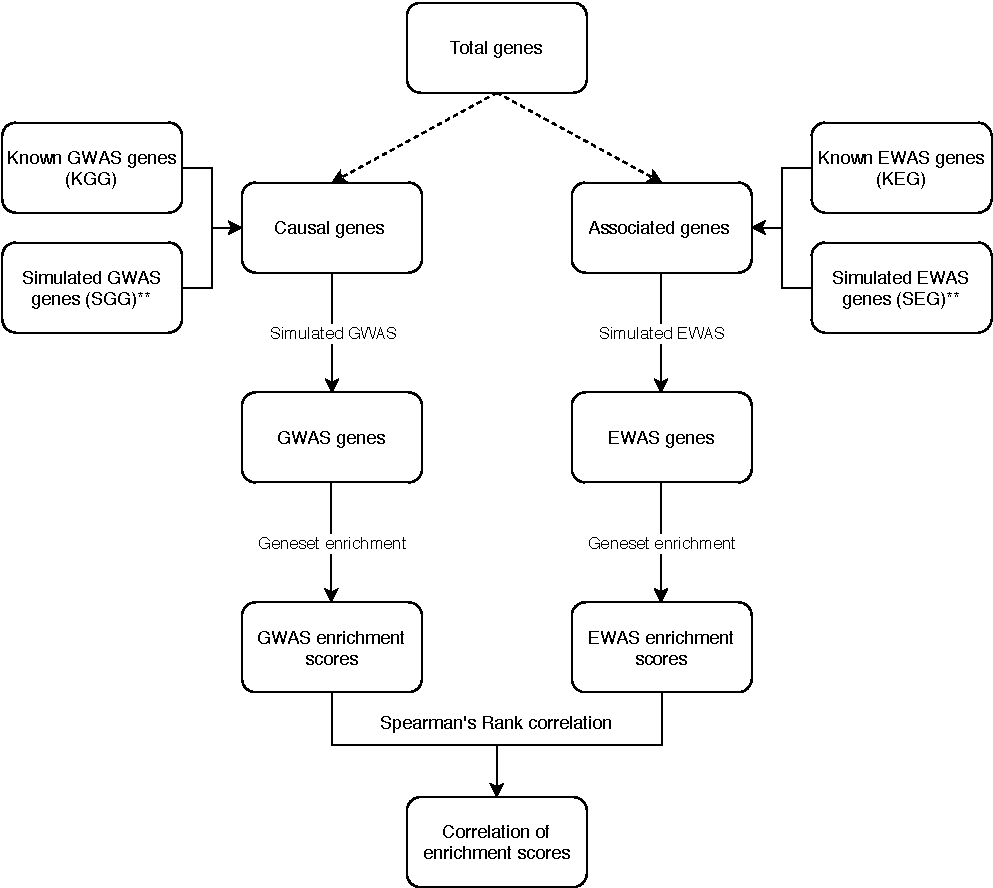
\includegraphics[width=1\linewidth]{figure/06-ewas_gwas_comparison/architecture-simulations-schematic} 

}

\caption[Flowchart demonstrating how the second set of simulations were set up for each trait]{\textbf{Flowchart demonstrating how the second set of simulations were set up for each trait.} Phenotypic variation may be caused by changes in gene/protein polymers (causal genes) and can be associated with changes in gene/protein polymers via other routes such as confounding or reverse causation (associated genes). In these simulations the causal genes were a mix of genes identified by GWAS, known GWAS genes (KGG), and a random set of genes, simulated GWAS genes (SGG). The associated genes were a mix of genes identified by EWAS, known EWAS genes (KEG), and a random set of genes, simulated EWAS genes (SEG). The level of overlap in the causal and associated genes was modified by changing the overlap in the SGG and SEG. The number of causal and associated genes was kept the same for each simulation, but this number varied between simulations. The minimum number of causal genes and the minimum number of associated genes was equal to the sum of KGG and KEG. The ``simulated GWAS'' step in the simulation simply equates to randomly sampling from the causal genes. The number of genes sampled was equal to the number of KGG. The ``simulated EWAS'' step was identical except the number of KEG from the associated genes. Geneset enrichment was performed as described in \textbf{Section \ref{methods-06}}. The simulations were repeated 1000 times for each set of parameters.}\label{fig:arch-simulations-schematic}
\end{figure}
From the simulations it was determined that, for seven of eight traits, it is likely that if the number of genes discovered currently is near to the total genes to discover for these traits, the proportion of overlap between causal and associated genes is low. However, for former vs.~never smoking, there was greatest evidence for a scenario where the causal and consequential gene overlap was high. The results from the analysis of former vs.~never smoking and c-reactive protein (representing simulations for the other traits) are shown in \textbf{Figure \ref{fig:arch-simulations-crp-fvns}}. \textbf{Figure \ref{fig:arch-simulations-supp-res}} shows the same results for the other traits. Each simulation was repeated 1000 times. Evidence for a difference in the empirically determined correlation of geneset enrichment scores and the mean correlation of geneset enrichment scores across simulations was assessed using a z-test for difference. There was some evidence against 53 simulation scenarios (FDR \textless{} 0.05). Across the traits, the scenarios that were least likely tended to be when the number of genes yet to discover was low, and the overlap between causal and associated genes was high, except for former vs.~never smoking, highlighting architecture differences between traits.




\begin{figure}

{\centering 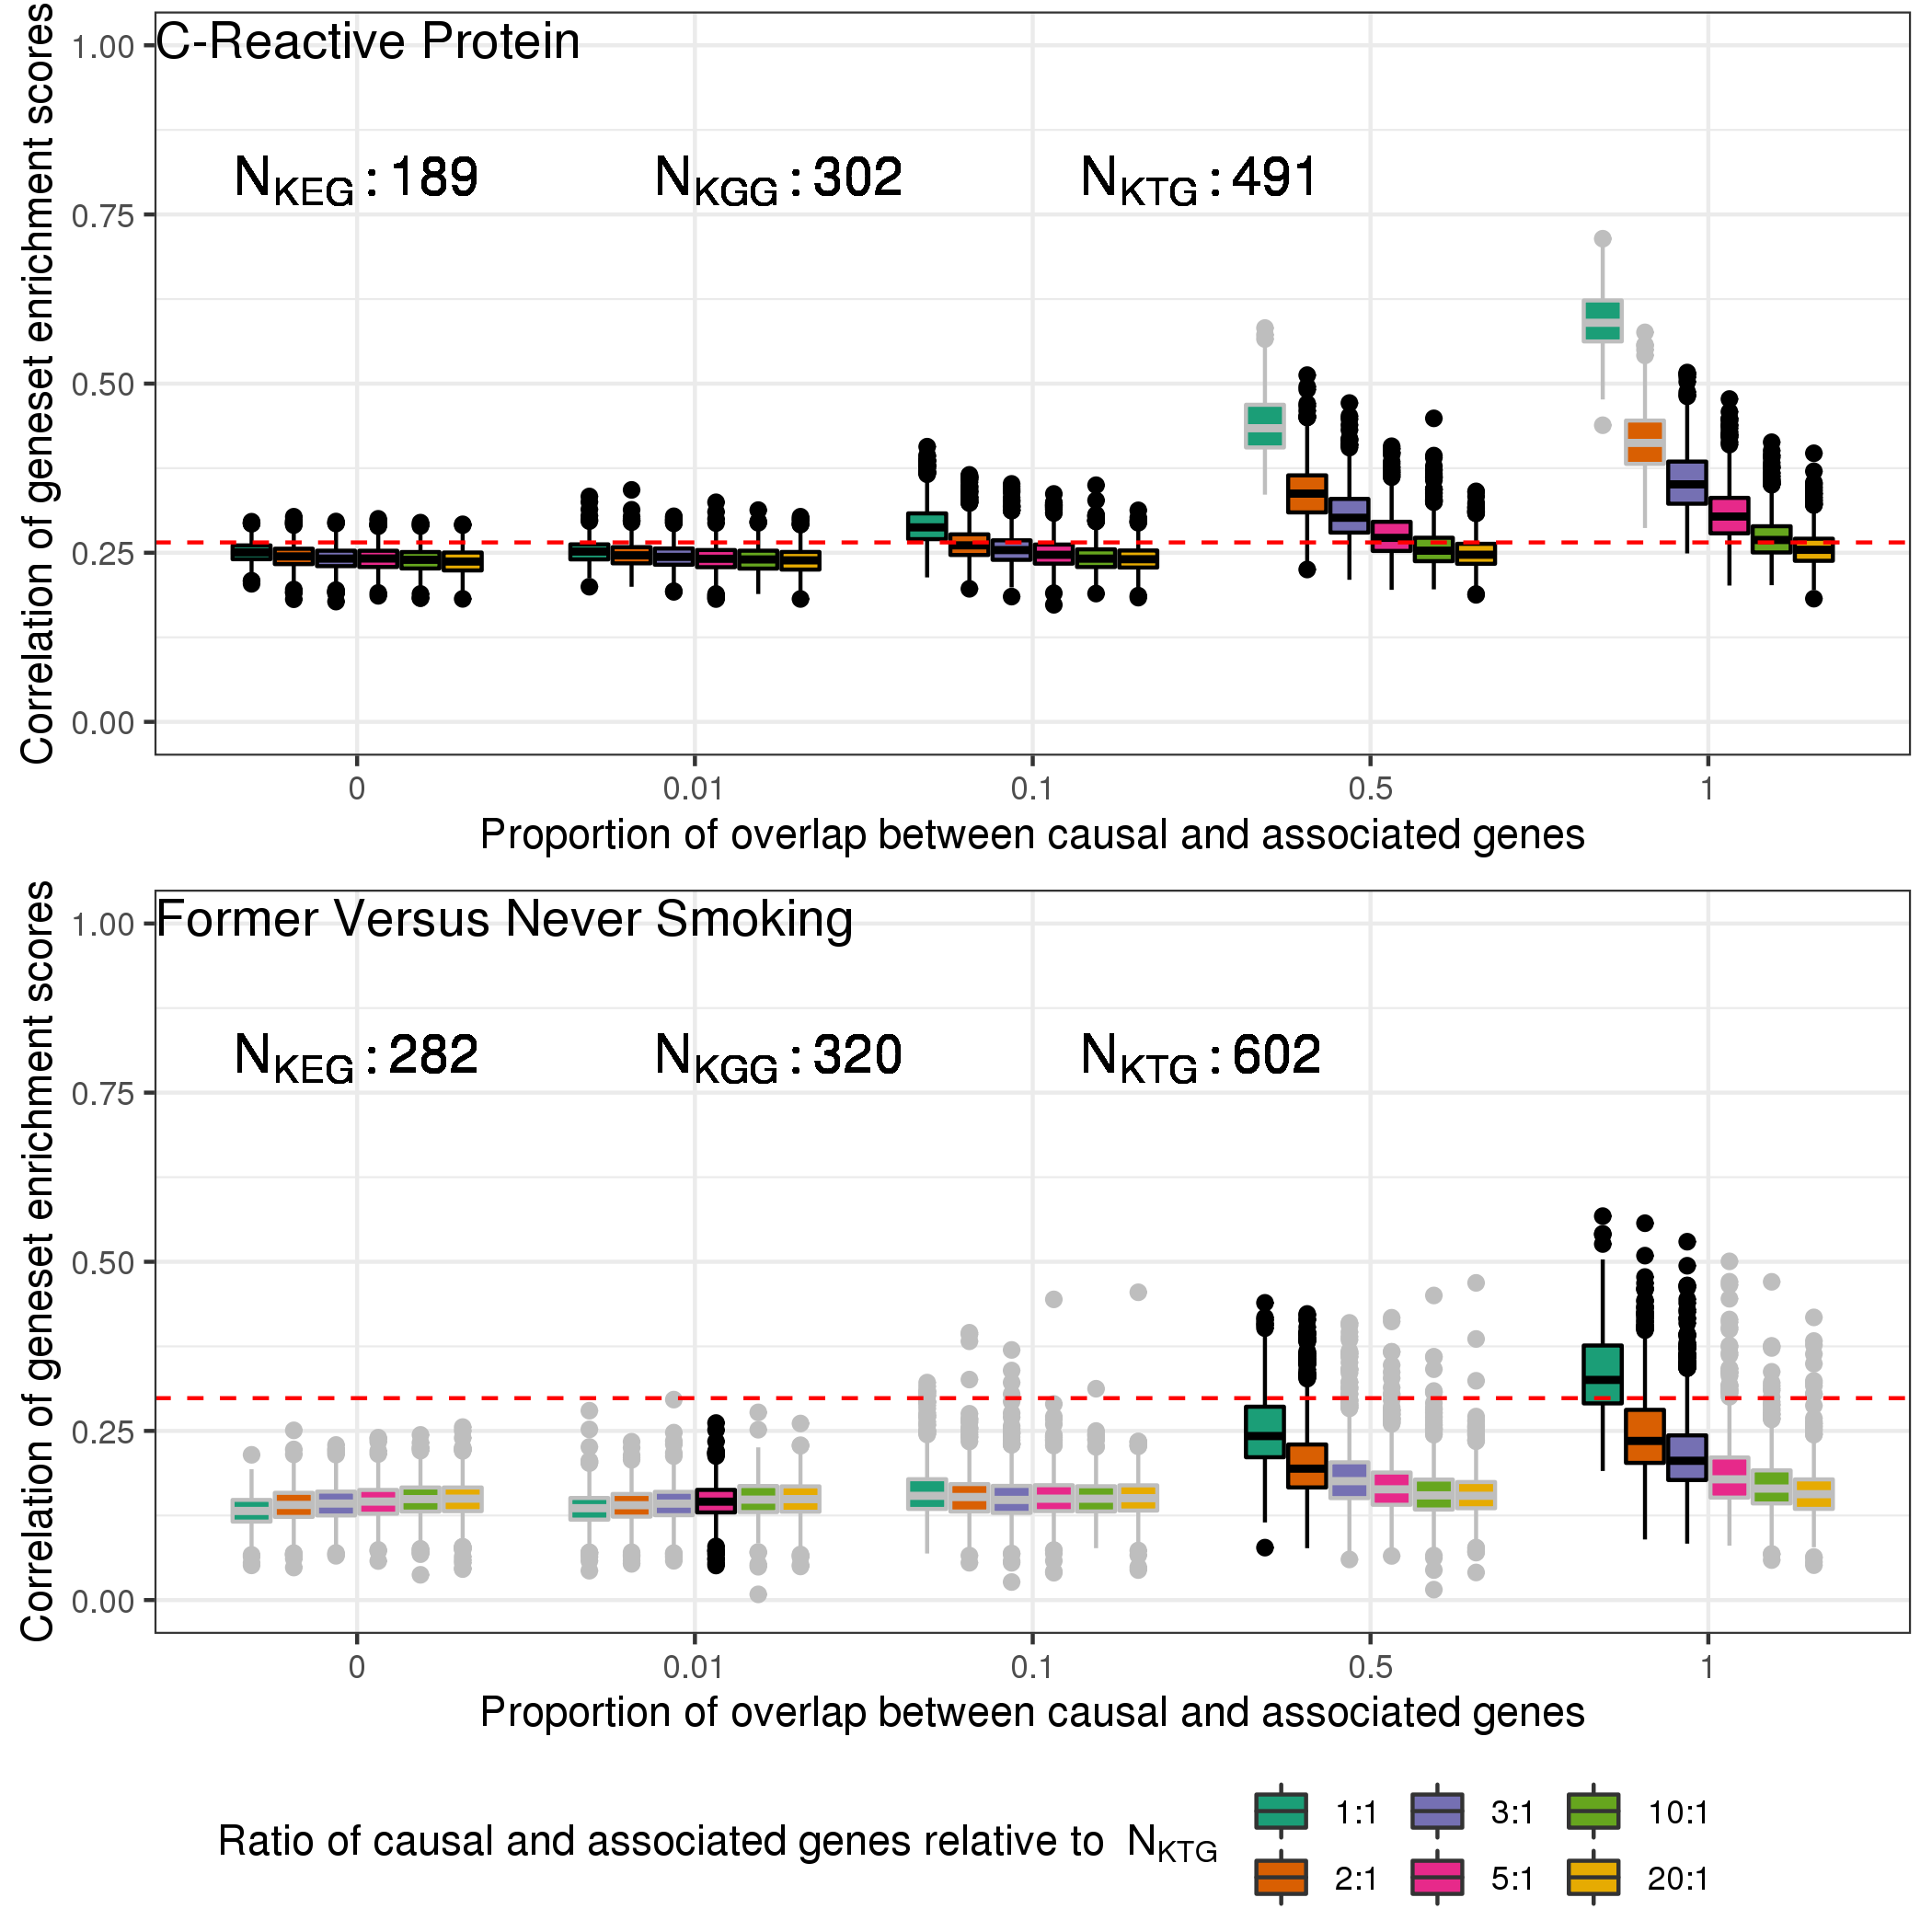
\includegraphics[width=1\linewidth]{figure/06-ewas_gwas_comparison/architecture_sims_crp_fvns_only_correlation_of_pathway_enrichment_scores} 

}

\caption[Simulations to understand the likely number of genes still to identify in EWAS and GWAS of c-reactive protein and smoking (former vs.~never smokers) under different trait architectures]{\textbf{Simulations to understand the likely number of genes still to identify in EWAS and GWAS of c-reactive protein and former vs.~never smoking under different trait architectures}. Simulations were set up as illustrated in \textbf{Figure \ref{fig:arch-simulations-schematic}}. Correlation of geneset enrichment scores from empirical data (\textbf{Table \ref{tab:empirical-pathway-tab}}), is shown as a red dashed line. Box plots show the range of enrichment score correlations from 1000 simulations using the parameters indicated. The number of causal and associated genes, as well as the overlap between these genes were varied. N\textsubscript{KEG} = number of known EWAS genes, N\textsubscript{KEG} = number of known GWAS genes, N\textsubscript{KTG} = number of known total genes (N\textsubscript{KEG} + N\textsubscript{KGG}). By way of an example, when N\textsubscript{KTG} = 491 and the ratio of causal and associated genes relative to N\textsubscript{KTG} is 1:1, the number of causal genes in the simulations will be 491 and the number of associated genes in the simulations will be 491. Scenarios which lie close to the empirical result (red dashed line) are more likely to reflect the true underlying number of genes related to a trait and the true overlap between the causal and associated genes. Where there is some evidence that the empirical results are different to the simulations (z-test FDR \textless{} 0.05) the box outline is grey.}\label{fig:arch-simulations-crp-fvns}
\end{figure}
\hypertarget{matching-gwas-to-ewas}{%
\subsection{Overlap of non-corresponding EWAS and GWAS}\label{matching-gwas-to-ewas}}

It may be the case that EWAS of one trait are actually more closely related to GWAS of another trait. For example, if DNA methylation changes related to BMI were mediating the effect of BMI on changes in metabolites, then one could expect to see greater correspondence in identified genes and genesets with GWAS of those metabolites.

To test if this was the case for any of the EWAS in this study, 1886 GWAS with SNPs associated at 5x10\textsuperscript{-8} with a sample size above 5000 from the IEU OpenGWAS Project (95) were extracted. For each GWAS and the eight EWAS, enrichment scores were calculated using geneset enrichment analysis and correlation between the enrichment scores was calculated, as in previous analyses.

Across all pairwise comparisons, correlations between enrichment scores ranged from -0.014 to 1 and had a mean of 0.12. The mean correlation between GWAS traits and EWAS traits was 0.23, which was higher than the correlations between just GWAS traits (0.12). Amongst just GWAS results, there was evidence that 14653 pairwise enrichment score correlations were greater than the the mean (FDR \textless{} 0.05). However, there was little evidence that any pairwise correlations between enrichment scores derived from EWAS and GWAS were greater than the mean correlation (FDR \textgreater{} 0.05).

This suggests that the signal from EWAS is not capturing aspects of any specific factor that impacts the aetiology of any of the eight traits of interest.

\hypertarget{discussion-06}{%
\section{Discussion}\label{discussion-06}}

Several EWAS papers have compared their findings with those of the corresponding trait GWAS (184,188--191), but it's unknown if any overlap that might occur should be attributed to shared underlying genetic and epigenetic architectures or if it occurs by chance. In this study, the genes and genesets identified by eight large EWAS (N\textgreater4500) were not identified in their corresponding GWAS any more than expected by chance. Simulations suggested these EWAS could still be identifying aspects of trait aetiology, but it is likely most DMPs identified are due to confounding or reverse causation. Further simulations suggested that the overlap between genes that impact phenotypic variation and those that might be identified through confounded analyses or reverse causation is likely to be low. However, if the number of genes still to identify in EWAS and GWAS is high, it is possible that the overlap between ``causal'' and ``associated'' genes could be high also.

\hypertarget{overlap-expected}{%
\subsection{Overlap expected}\label{overlap-expected}}

GWAS identifies the effects of genetic variation on complex traits. These effects are less likely to be confounded than associations estimated between observational phenotypes (92,93). Thus, one would expect overlap between genes and gemesets identified by EWAS and GWAS of the same trait if the DMPs identified are also of aetiological relevance. Assuming mapping of DMPs and SNPs to genes is correct, the genes identifed by EWAS may cause variation in complex traits without overlapping with genes identified in GWAS. Under the scenario where the effect of a SNP on a complex trait is mediated by a distal DNA methylation site (or the gene that site is tagging), GWAS and EWAS may identify genes that do not overlap, but that are along the same causal pathway from genome to complex trait. One plausible mechanism for which trans-mQTLs may act is via transcription factors. A trans-mQTL may influence the transcription of a nearby transcription factor then the transcription factor could cause a change in DNA methylation at distal sites. One study has provided evidence this may occur frequently (120). In this scenario the genes proximal to the identified SNP and DMP would lie on the same causal pathway and so would likely be part of the same genesets. This is likely not the only plausible mechanism of trans-mQTL function though. DNA methylation may also mediate non-genetic effects, allowing for causal DMPs to be identified at genes not near pertinent genetic variation. However, there is strong evidence that the majority of DNA methylation sites have a heritable component. As such any effect of DNA methylation on a trait could be influenced by genetic variation. If DNA methylation is influenced by proximal genetic variants then the discovery of the same gene(s) will be a function of GWAS and EWAS power. If only distal genetic variants influence the DNA methylation site, then the overlap of genesets is a function of regulatory mechanisms and power. These two issues, and likely others, may introduce noise into the results. However, there is overwhelming evidence that confounding and reverse causation are pervasive across observational epidemiology (192--195) as well as within EWAS (1,196). This suggests that the evidence that EWAS and GWAS are not identifying any more overlapping genes and genesets than expected by chance, is likely due to identified DMPs being mostly the result of reverse causation or confounding.

As the simulations showed, even if an EWAS identifies DMPs that cause a change in the trait, if the majority of DMPs identified are due to confounding or reverse causation then the overlap will be indistinguishable to the overlap expected by chance. Thus, our empirical results do not preclude the possibility that some DMPs identified by the EWAS are pertinent to trait aetiology.

For body mass index, work has already suggested the traits cause changes in DNA methylation rather than \emph{vice versa} (70,73), supporting our findings here. Further, one study suggested DNA methylation changes capture different components of body mass index variance than genetic variation (60) and another estimated the percentage of trait variance captured by DNA methylation was 75.7\% when accounting for genotype (177).

Simulations involving empirical data from former vs.~never smoking EWAS and GWAS suggested that overlap between causal and associated genes was high. This is surprising for two reasons. Firstly, it differs from the current vs.~never smoking results, suggesting distinct genetic or epigenetic architectures of those traits. Secondly, there is evidence that for DNA methylation changes identified in relation to smoking, smoking is likely causing DNA methylation variation and not \emph{vice versa}. Although the statistical tests suggested that it was unlikely that the proportion of causal and associated genes is 0.1 or lower, it should be noted that the absolute difference between simulated results and empirical results were not great.

If EWAS is discovering some DMPs that influence genes that cause changes in the trait of interest, study power is the limiting factor for detecting overlap. For traits with a weak polygenic architecture (few genes explain most of the heritability), such as gene expression (197,198), discovering almost total overlap would be inevitable even with modest sample sizes.

\hypertarget{little-overlap-with-any-gwas}{%
\subsection{Little overlap with any GWAS}\label{little-overlap-with-any-gwas}}

Little correlation was found between geneset enrichment scores for EWAS and GWAS of non-corresponding traits. In a scenario where DNA methylation was capturing a specific facet of a trait one might expect correlation between EWAS of the original trait and GWAS of that facet. For example, if changes in DNA methylation associated with smoking were mostly responsible the effect of smoking on lung cancer then one would expect to observe an overlap between the genes and pathways identified by an EWAS of smoking and GWAS of lung cancer. This specific example is explored, in part, in \textbf{Chapter \ref{dnam-lung-cancer-mr}} under a Mendelian randomization framework and has been examined before, with a study suggesting methylation at two sites (of over 1000 smoking-related sites) mediate over 30\% of the effect of smoking on lung cancer (199). The results of either study suggest most sites will not mediate the effect of smoking on lung cancer and thus there would be little overlap between genes and pathways of an EWAS of smoking and a GWAS of lung cancer. This is corroborated by the results of our study: there was little evidence that correlation of pathway enrichment scores between the two, 0.15, was greater than the mean correlation enrichment score across all GWAS-GWAS and GWAS-EWAS correlations, 0.12 (FDR \textgreater{} 0.05).

It is important to note that overlap between EWAS and GWAS genesets may be missed even if this mediation model is true for various traits. As shown in the simulations, detecting this overlap depends on individual study power as well as the underlying genetic and epigenetic architecture of the trait. There are further things that may limit detection of geneset overlap that is discussed later on.

\hypertarget{information-gained}{%
\subsection{Information gained from EWAS}\label{information-gained}}

The fact that genes and pathways identified from GWAS and EWAS of the same traits are seemingly very separate suggests we are gaining new information from EWAS, even if interpreting the new information may be difficult. Key to interpreting the EWAS results would be to try and disentangle whether the EWAS results are likely due to confounding (as is explored in \textbf{Chapter \ref{dnam-lung-cancer-mr}}). Interpreting EWAS can also be difficult due to cell type heterogeneity and the complexity of mechanisms which mediate DNA methylation changes (1,18,45,78,79). Due to these difficulties it should not be concluded that EWAS definitely help increase our biological understanding of complex traits. Rather, DNA methylation is capturing different biological information. Regardless of biological insight gained, translational impact may still be gleaned from DNA methylation studies; DNA methylation may aid diagnoses by acting as a reliable biomarker or could help predict various health outcomes (49).

There are also benefits to understanding the biological consequences of a trait, something that EWAS might help identify and GWAS will not (at least not directly). This does depend on further research to understand how changes in DNA methylation downstream to complex trait variation is relevant to human health. Further, establishing where exactly DNA methylation may lie on the causal pathway may be difficult and work is ongoing to discover this for various traits (118). Use of causal inference methods such as Mendelian randomization (92,93,116) can be applied (and are in \textbf{Chapter \ref{dnam-lung-cancer-mr}}), but this still comes with various caveats, as discussed in \textbf{Section \ref{establishing-causality}} (116,118). Some studies also try and confirm effects experimentally (66) and use previous biological knowledge of the trait to try and understand EWAS results.

However, some of the biological knowledge of complex traits relating to genes and pathways comes from GWAS of those traits. This study suggests that EWAS is unlikely to identify many genes proximal to genetic variation pertinent to the trait of interest and further the genesets are unlikely to overlap with those identified in GWAS. Therefore, comparison of EWAS results to those of a corresponding GWAS is unlikely to explain a large proportion of DNA methylation-trait associations observed in EWAS. This may make inference from EWAS difficult, yet it seems likely the interpretability of DNA methylation studies will continue to improve over the coming years, as understanding the underlying epigenetic architecture of complex traits could still provide translational benefits (49).

\hypertarget{limitations-06}{%
\subsection{Limitations}\label{limitations-06}}

As discussed, detecting gene or pathway overlap depends on the genetic and DNA methylation architecture of the trait. Here only eight traits, two of which are smoking behaviour traits, have been studied. This means the results cannot be generalised to all or even the majority of complex traits. These analyses could be repeated by setting a less restrictive sample size limit, but it was felt that would make the results less reliable and impossible in many circumstances where too few DNA methylation sites had been discovered by EWAS. As sample sizes increase and technologies measuring more DNA methylation sites become more common, it would be interesting to repeat the analysis.

Often in GWAS and EWAS, prioritisation of SNPs and DMPs identified occurs before functional mapping. Prioritsation for both studies may be informed by prior knowledge of the trait, prior understanding of molecular biology, predicted consequences of observed variation (for example using Ensembl's Variant Effect Predictor (200)), replication of findings or a number of other methods. In this study, I did not perform any prioritisation (besides the conventional P value threshold cutoffs) and thus may have increased the amount of ``noise'' in the signal taken forward for functional annotation. Unfortunately, this extra prioritisation of sites is not tractable when comparing many different association studies and may reduce power to detect any overlap between genes and pathways. However, added noise is unlikely to prevent detection of true overlap if that true overlap is substantial, as shown by the simulations (\textbf{Figure \ref{fig:sim1-summ-plot}}).

The nearest gene, by chromosomal position, to a DMP or SNP is not necessarily the gene of interest. SNPs may have effects on genes distal to their position (201). Also, the correlation between genetic variants inflates associations of variants proximal to the true causal variant, which may map to unrelated genes. Further, the correlation structure in DNA methylation data may induce associations between complex traits at a site far from where variation in DNA methylation causes complex trait changes (201). Therefore, the mapping of DMPs and SNPs to genes in this study could likely be improved. The ``correct'' method for this mapping has not yet been established though and even though some tools are available (such as eQTL studies), there are caveats to them too (202,203).

Our understanding of molecular pathways is not complete and thus attributing genes to certain pathways or functionalities may be erroneous. However, the results remained consistent across four different methods that annotate genes to pathway, suggesting differences in mapping genes to genesets should not impact our conclusions.

Biological information gained from EWAS and GWAS may be defined in various ways and depending on the interpretation of this, one could alter methods used to extract biological information. However, first exploring the genomic regions identified and then mapping these to potentially relevant biological genesets is common amongst GWAS and EWAS (167,179,182--185,204) and gave a simple way to compare the information from the two study types.

\hypertarget{conclusion-06}{%
\section{Conclusion}\label{conclusion-06}}

Overall this chapter provides evidence that, for eight complex traits, there is little overlap between genes and genesets identified by EWAS and GWAS of the same trait. Given the differences in properties between DNA methylation and genetic variants the results presented in this study may apply to other traits, but this is still to be confirmed. Where lack of overlap between genes and genesets is found, it suggests EWAS may be providing new biological information, however, the interpretability of EWAS is still in question and with current methods it is hard to determine if EWAS results are attributable to confounding or reverse causation. Regardless, as causal inference within epigenetic epidemiology improves, it seems likely we will be able to interpret this apparent gain in biological information.

\hypertarget{methods-06}{%
\section{Methods}\label{methods-06}}

\hypertarget{samples-06}{%
\subsection{Samples}\label{samples-06}}

EWAS summary data and GWAS summary data were extracted from the EWAS Catalog (\textbf{Chapter \ref{ewas-catalog}}) and the IEU OpenGWAS Project (95,96) respectively. The data was extracted in July 2019, when the EWAS Catalog contained data published before 2019. For traits that had multiple EWAS with a sample size of greater than 4500, the EWAS with the largest sample size was used, the same was applied to the GWAS. The sample size, first authors and PubMed IDs can be found in \textbf{Table \ref{tab:trait-data-tab-06}}.

\hypertarget{overlapping-genomic-regions}{%
\subsection{Overlapping genomic regions}\label{overlapping-genomic-regions}}

Each chromosome was divided into 500Kb blocks, each block that did not contain a DNA methylation site measured by the HM450 was removed. For each trait, the genome blocks that had one or more EWAS sites and one or more GWAS sites that reached the set p-value threshold were tallied. The p-value threshold was set at a lenient P \textless{} 1x10\textsuperscript{-5} or if it was lower, the maximum reported p-value in the EWAS of that trait.

\hypertarget{mapping-sites-to-genes-and-genesets}{%
\subsection{Mapping sites to genes and genesets}\label{mapping-sites-to-genes-and-genesets}}

The R package biomaRt (205) was used to extract Ensembl gene ids along with chromosome positions of all genes. The package was also used to extract gene ontology (GO) terms (206,207) and map these to the Ensembl gene ids. The R package limma (86) was used to extract KEGG terms (208,209,209) and these were mapped to Ensembl gene ids.

Protein-protein interaction data, which includes data from StringDB (210) and IntAct (211), and terms from the Reactome database (212) were extracted from \href{http://www.epigraphdb.org/}{EpiGraphDB} (213).

CpG sites associated with traits at P \textless{} 1x10\textsuperscript{-7} and SNPs associated with traits at P \textless{} 5x10\textsuperscript{-8} were taken forward to be mapped to genes. The correlation structure present in genetic and DNA methylation data makes it difficult to ascertain the precise site driving any signal observed. Thus, no filtering based on correlation between variants or CpG sites was performed.

For each CpG site identified by EWAS and used in the analyses, it was mapped to the nearest gene (Ensembl gene ID) by chromosome position. If a CpG site lay within the bounds of multiple genes then the site was mapped to all of those genes. Therefore, one CpG site could map to multiple genes and one gene could map to multiple CpG sites. The same gene mapping approach was used for variants identified in GWAS. The positions of CpG sites were extracted using the R package meffil (149).

\hypertarget{methods-for-assessing-overlap}{%
\subsection{Methods for assessing overlap}\label{methods-for-assessing-overlap}}

To test the overlap between genes identified we generated ORs as follows
\begin{equation}
    OR_{gene-overlap} = \frac{odds_{EG}} {odds_{EnG}}
    \label{eq:overlap-of-genes}
\end{equation}
where \(odds_{EG}\) is the odds of a gene being identified in EWAS and GWAS and \(odds_{EnG}\) is the odds of a gene being identified in EWAS, but not in GWAS.

Genes may map to genesets by chance. Often in EWAS and GWAS, enrichment for any genesets are tested by assessing whether the genes identified are more common in any geneset than expected by chance. Power was compared between mapping genes to genesets and directly assessing overlap like in Equation \eqref{eq:overlap-of-genes} and correlation between enrichment scores for each geneset. Enrichment scores are also odds ratios generated in a similar way to those in Equation \eqref{eq:overlap-of-genes}:
\begin{equation}
    OR_{geneset-enrichment} = \frac{odds_{GS}} {odds_{nGS}}
    \label{eq:geneset-enrichment}
\end{equation}
where \(odds_{GS}\) is the odds of a gene being annotated to the geneset and \(odds_{nGS}\) is the odds of a gene not being annotated to the geneset.

For many genesets, genes annotated to that geneset would not be identified in an EWAS or GWAS, causing the enrichment score for many genesets to be zero. Further, some genesets would have very large enrichment scores. This made the relationship between enrichment scores generated for the EWAS results and the enrichment scores generated for the GWAS non-normal. Thus, to examine the relationship between the two, Spearman's rank correlation coefficients of the logarithm of enrichment scores was used.

\hypertarget{testing-power-to-detect-overlap}{%
\subsection{Testing power to detect overlap}\label{testing-power-to-detect-overlap}}

Simulations were setup as seen in \textbf{Figure \ref{fig:method-simulations-schematic}}. The simulations iterated over each set of parameters 1000 times. For each iteration, two sets of genes, GWAS genes and EWAS genes, were sampled from the total set of genes. Each iteration assessed gene overlap and geneset overlap between these gene sets using Equation \eqref{eq:overlap-of-genes}. Equation \eqref{eq:geneset-enrichment} was used to generate enrichment scores for each gene set and then correlation between the enrichment scores was assessed.

GWAS genes were only sampled from a set of ``causal'' genes and a proportion of EWAS genes were sampled from the set of causal genes and the rest from the set of ``associated'' genes. Receiver operator characteristic (ROC) curves were generated to assess whether it was possible to predict the gene overlap, geneset overlap and enrichment score correlations for scenarios where the proportion of causal EWAS genes was greater than zero from the scenario where the proportion of causal EWAS genes was zero. The area under these ROC curves were then calculated in each case.

These simulations were repeated for each geneset and protein-protein interaction database. The protein-protein interaction and Reactome databases all map only to protein coding genes, whereas the GO and KEGG databases map to all Ensembl gene IDs. To compare predictive ability across annotation methods, Ensembl gene IDs that were not protein coding genes were excluded. A comparison between the performance of models when mapping to all Ensembl gene IDs or to protein coding genes was made for GO and KEGG databases. (\textbf{@ref(fig:sim1-go-kegg-gene-comp5}).

From these simulations, the best method to assess geneset overlap, and the best geneset annotation method to assess that overlap and the scenarios (i.e.~study power required, proportion of DMPs that need to be causal) in which it could be expected to be able to detect overlap could be deduced.

\hypertarget{empirical-analyses}{%
\subsection{Empirical analyses}\label{empirical-analyses}}

The DNA methylation sites identified in the EWAS at P \textless{} 1x10\textsuperscript{-7} and the SNPs identified in the GWAS at P \textless{} 5x10\textsuperscript{-8} were mapped to genes and genesets. Overlap between genes was calculated as before (Equation \eqref{eq:overlap-of-genes}), enrichment scores were generated and correlated as described above.

Expected overlap was generated to compare to the observed results. For this, random positions were chosen in the genome equal to the number of DMPs identified in the EWAS. These genes were then used to assess gene and geneset overlap as for the observed results. This was repeated 1000 times to generate a null distribution and a z-test was used to assess whether there was a difference between the observed results and the mean of the null distribution.

There is a correlation structure within DNA methylation data (214), and it was hypothesised this might contribute to the observed results. By randomly sampling positions from the genome, a new correlation structure between DMPs would be generated. I tested whether sampling the genome in a non-random way, aimed at keeping some correlation structure, altered the results. To generate new data whilst attempting to keep a similar correlation structure, a fixed number of base pairs were added to each of the DMPs identified in the empirical analysis such that
\begin{equation}
    BP_{new} = BP_{dmp} + max(G) \times I
    \label{eq:generating-new-positions}
\end{equation}
where \(BP_{new}\) = base pair of new site, \(BP_{dmp}\) = base pair of DMP identified in the EWAS, \(G\) = gene size, and \(I\) = iteration.

If \(BP_{new}\) extended beyond the end of a chromosome, the position moved onto the next chromosome, with positions moving past the end of chromosome 22, being moved to chromosome 1.

Overall, the overlap between genes and genesets identified by EWAS and GWAS did not change across null distribution sampling methods.

\hypertarget{architecture-sims-method}{%
\subsection{Understanding architecture from geneset overlap}\label{architecture-sims-method}}

Simulations were setup as illustrated in \textbf{Figure \ref{fig:arch-simulations-schematic}}. Here I describe simulations for a single trait. These were repeated for all traits. Firstly, SNPs identified in GWAS and DMPs identified in EWAS were mapped to genes as described in \textbf{Section \ref{gwas-ewas-overlap}}. Genes were then randomly sampled from Ensembl gene IDs and were assigned as either ``causal'', meaning changes in that gene effect variation in the phenotype across individuals, or ``associated'', meaning changes in the gene are associated with the phenotype across individuals, but the nature of association is not known. The empirically identified (or ``known'') GWAS genes (\(KGG\)) were added to the list of causal genes and the empirically identified (or ``known'') EWAS genes (\(KEG\)) were added to the list of associated genes. These combined set of causal and associated genes can be thought of as all the genes related to the trait of interest. A number of genes, equal to the number of \(KGG\) (\(N_{KGG}\)), was sampled from the causal set of genes and assigned to be the ``GWAS genes'' in the simulations. A number of genes, equal to the number of \(KEG\) (\(N_{KEG}\)), was sampled from the associated set of genes and assigned to be the ``EWAS genes'' in the simulations. Then geneset enrichment analyses for both the EWAS and GWAS genes were performed (equation \eqref{eq:geneset-enrichment}) and correlation between the enrichment scores was assessed as previously. In these simulations, the number of total genes was varied and the number of causal and associated genes was always set to be half of the total number of genes related to a trait. The total number of genes was proportional to the total number of known genes (\(N_{KTG} = N_{KGG} + N_{KEG}\)). The smallest number of total genes for any simulation was double the number of \(N_{KTG}\) and the greatest number of total genes was 40 times \(N_{KTG}\). The other variable set to vary between simulations was the proportion of overlap between causal and associated genes. This varied between zero and one, where zero represented the scenario where only the overlap in \(KGG\) and \(KEG\) would be present in the overlap between causal and associated genes and one represented the scenario where all causal and associated genes were the same. For each simulation scenario, the simulations were repeated 1000 times and box plots show the range of output from those 1000 repeats.

\hypertarget{assessing-the-correlation-between-geneset-enrichment-results}{%
\subsection{Assessing the correlation between geneset enrichment results}\label{assessing-the-correlation-between-geneset-enrichment-results}}

GWAS were extracted from the IEU OpenGWAS Project (95) with the following criteria:
\begin{itemize}
\tightlist
\item
  Sample size \textgreater{} 5000
\item
  European population
\item
  For binary traits, cases and controls had to be greater than 500
\item
  Full genome-wide results, i.e.~not just associations between a molecular trait and variants in cis.
\end{itemize}
For each GWAS, all SNPs that associated with the trait at P\textless5x10\textsuperscript{-8} were extracted. CpGs associated with the eight EWAS at P\textless1x10\textsuperscript{-7} were then extracted and mapped to genes. For each study, enrichment scores were generated for GO terms as before (Equation \eqref{eq:geneset-enrichment}) and correlation between them assessed.

When assessing whether gene overlap or geneset enrichment score correlations were greater than the mean, a z-test was performed. As multiple tests were performed we applied the Benjamini-Hochberg method (215) to limit the false discovery rate.

\hypertarget{dnam-lung-cancer-mr}{%
\chapter{Appraising the causal relevance of DNA methylation for risk of lung cancer}\label{dnam-lung-cancer-mr}}

\hypertarget{chapter-summary-07}{%
\section{Chapter summary}\label{chapter-summary-07}}

The results of \textbf{Chapter \ref{ewas-gwas-comp-chapter}} suggested that epigenome-wide association studies (EWAS) might be identifying differential facets of complex trait biology when compared to genome-wide association studies (GWAS) of corresponding traits. As discussed in \textbf{Section \ref{problems-for-ewas}}, observational studies such as EWAS suffer from issues of reverse causation and confounding, which could have explained the results in \textbf{Chapter \ref{ewas-gwas-comp-chapter}}.

In this chapter I attempt to explore the extent to which EWAS results may be confounded. To acheive this I first perform a meta-analysis of lung cancer EWAS and then compare the results from this observational analysis to the same analysis in a well-powered Mendelian randomization (MR) framework. DNA methylation has recently been postulated to mediate over 30\% of the effect on smoking on lung cancer (199), making this case of particular interest to potential lung cancer preventative stratergies.

\hypertarget{introduction-07}{%
\section{Introduction}\label{introduction-07}}

Lung cancer is the most common cause of cancer-related death worldwide (216). Several DNA methylation changes have been recently identified in relation to lung cancer risk (125,199,217). However, these epigenetic marks are sensitive to reverse causation, being affected by cancer processes (218), and are also prone to confounding, for example by socio-economic and lifestyle factors (143,219).

One CpG site, cg05575921 within the aryl hydrocarbon receptor repressor (\emph{AHRR}) gene, has been consistently replicated in relation to both smoking (68) and lung cancer (105,125,199) and functional evidence suggests that this region could be causally involved in lung cancer (144). However, the observed association between methylation and lung cancer might simply reflect separate effects of smoking on lung cancer and DNA methylation, i.e.~the association may be a result of confounding (108), including residual confounding after adjustment for self-reported smoking behaviour (195,220). Furthermore, recent EWAS of lung cancer have revealed additional CpG sites which may be causally implicated in development of the disease (125,199).

As discussed in \textbf{Section \ref{establishing-causality}}, Mendelian randomization (MR) can be used to help infer causality in associations between DNA methylation and complex traits (116,181,221) under a paradigm that largely mitigates the problem of confounding if certain assumptions are met (\textbf{Figure \ref{fig:mr-diagram}}).

In this study, I performed a meta-analysis of four lung cancer EWAS (918 case-control pairs) from prospective cohort studies to identify CpG sites associated with lung cancer risk and applied MR to investigate whether the observed DNA methylation changes at these sites are causally linked to lung cancer.

\hypertarget{methods-07}{%
\section{Methods}\label{methods-07}}

\hypertarget{ewas-study-details}{%
\subsection{EWAS study details}\label{ewas-study-details}}

A meta-analysis of four lung cancer case-control EWAS was conducted to identify DNA methlyation sites associated with lung cancer. In total there were 918 cases and 918 matched controls for the analysis. A description of the studies, how controls were matched to cases and an outline of the study populations, laboratory methods, data pre-processing and quality control methods can be found in \textbf{Section \ref{lc-ewas-data}} and they described in detail elsewhere (125).

\hypertarget{methods-ewas-meta-analysis}{%
\subsection{EWAS Meta-analysis}\label{methods-ewas-meta-analysis}}

To quantify the association between the methylation level at each CpG and the risk of lung cancer conditional logistic regression models were fitted for beta values of methylation (which ranges from 0 (no cytosines methylated) to 1 (all cytosines methylated)) on lung cancer status for the four studies. Surrogate variables were computed in the four studies using the SVA R package (222) and the proportion of CD8+ and CD4+ T cells, B cells, monocytes, natural killer cells and granulocytes within whole blood were derived from DNA methylation (78). The following EWAS models were included in the meta-analysis: Model 1 -- unadjusted; Model 2 -- adjusted for 10 surrogate variables (SVs); Model 3 -- adjusted for 10 SVs and derived cell proportions. EWAS stratified by smoking status was also conducted (never (N=304), former (N=648) and current smoking (N=857)). For Model 1 and Model 2, the case-control studies not matched on smoking status (EPIC-Italy and NOWAC) were adjusted for smoking.

An inverse-variance weighted fixed effects meta-analysis was performed of the EWAS (918 case-control pairs) using the \href{http://csg.sph.umich.edu/abecasis/metal/}{METAL software}. Direction of effect, effect estimates and the I\textsuperscript{2} statistic were used to assess heterogeneity across the studies in addition to effect estimates across smoking strata (never, former and current). All sites identified at a false discovery rate (FDR) \textless{} 0.05 in Model 2 and 3 were also present in the sites identified in Model 1. The effect size differences between models for all sites identified in Model 1 were assessed by a Kruskal-Wallis test and a post-hoc Dunn's test. There was little evidence for a difference (P \textgreater{} 0.1), so to maximize inclusion into the MR analyses sites identified in the unadjusted model (Model 1) were taken forward.

\hypertarget{methods-mendelian-randomization-07}{%
\subsection{Mendelian randomization}\label{methods-mendelian-randomization-07}}

Two-sample MR was used to establish potential causal effect of differential methylation on lung cancer risk (114,115).

\hypertarget{sample-1-accessible-resource-for-integrated-epigenomic-studies-aries}{%
\subsubsection{Sample 1: Accessible Resource for Integrated Epigenomic Studies (ARIES)}\label{sample-1-accessible-resource-for-integrated-epigenomic-studies-aries}}

In the first sample, mQTL-methylation effect estimates (\(\beta_{GP}\)) for each CpG site of interest were identified in an mQTL database from the Accessible Resource for Integrated Epigenomic Studies (ARIES) (\url{http://www.mqtldb.org}). Details on the methylation pre-processing, genotyping and quality control (QC) pipelines are described in \textbf{Section \ref{aries-02}}.

\hypertarget{sample-2-transdisciplinary-research-in-cancer-of-the-lung-and-the-international-lung-cancer-consortium}{%
\subsubsection{Sample 2: Transdisciplinary Research in Cancer of the Lung and The International Lung Cancer Consortium}\label{sample-2-transdisciplinary-research-in-cancer-of-the-lung-and-the-international-lung-cancer-consortium}}

In the second sample, summary data was extracted from a GWAS meta-analysis of lung cancer risk conducted by the TRICL-ILCCO consortium (29,863 cases, 55,586 controls). A brief description of the data can be found in \textbf{Section \ref{tricl-ilcco-02}}. This summary data was used to obtain mQTL-lung cancer estimates (\(\beta_{GD}\)).

For each independent mQTL (r\textsuperscript{2} \textless{} 0.01), I calculated the log OR per SD unit increase in methylation by the formula \(\frac{\beta_{GD}} {\beta_{GP}}\) (Wald ratio). Standard errors were approximated by the delta method (223). Where multiple independent mQTLs were available for one CpG site, these were combined in a fixed effects meta-analysis after weighting each ratio estimate by the inverse variance of their associations with the outcome. Heterogeneity in Wald ratios across mQTLs was estimated using Cochran's Q test, which can be used to indicate horizontal pleiotropy (224). Differences between the observational and MR estimates were assessed using a Z-test for difference.

If there was evidence for an mQTL-CpG site association in ARIES in at least one time-point, it was assessed whether the mQTL replicated across time points in ARIES (FDR \textless{} 0.05, same direction of effect). Further, this association was re-analysed using linear regression of methylation on each genotyped SNP available in an independent cohort (NSHDS), using RVTESTS (225). The same NSHDS samples on which DNA methylation was measured were genotyped using the Illumina Infinium OncoArray-500k BeadChip (Illumina Inc.~San Diego, CA) and quality control parameters were applied under the recently published TRICL-ILCCO GWAS study on lung cancer (130). Genetic imputation was performed on these samples using the Haplotype Reference Consortium (HRC) Panel (release 1) (217) through the Michigan Imputation Server (226). Replicated mQTLs were included where possible to reduce the effect of winner's curse using effect estimates from ARIES. The instrument strength of the mQTLs were assessed by the variance explained in methylation by each mQTL (r\textsuperscript{2}) as well as the F-statistic in ARIES \textbf{Table \ref{tab:sup-tab1-07}}. The power to detect the observational effect estimates in the two-sample MR analysis was assessed \emph{a priori}, based on an alpha of 0.05, sample size of 29,863 cases and 55,586 controls (from TRICL-ILCCO) and calculated variance explained (r\textsuperscript{2}). \linebreak
\begin{table}[!h]

\caption{\label{tab:sup-tab1-07}Instrument strength in ARIES}
\centering
\resizebox{\linewidth}{!}{
\begin{tabular}[t]{llllllll}
\toprule
SNP & CpG & Beta & SE & P & N & F & r\textsuperscript{2}\\
\midrule
\cellcolor{gray!6}{rs1048691} & \cellcolor{gray!6}{cg23387569} & \cellcolor{gray!6}{0.35} & \cellcolor{gray!6}{0.053} & \cellcolor{gray!6}{3.9e-11} & \cellcolor{gray!6}{834} & \cellcolor{gray!6}{45} & \cellcolor{gray!6}{0.05}\\
rs1939110 & cg11660018 & -0.40 & 0.048 & 2.6e-16 & 834 & 70 & 0.08\\
\cellcolor{gray!6}{rs13087163} & \cellcolor{gray!6}{cg01901332} & \cellcolor{gray!6}{-0.19} & \cellcolor{gray!6}{0.035} & \cellcolor{gray!6}{5.8e-08} & \cellcolor{gray!6}{834} & \cellcolor{gray!6}{30} & \cellcolor{gray!6}{0.03}\\
rs7927381 & cg01901332 & 0.38 & 0.069 & 3.9e-08 & 834 & 31 & 0.04\\
\cellcolor{gray!6}{rs878481} & \cellcolor{gray!6}{cg05951221} & \cellcolor{gray!6}{-0.32} & \cellcolor{gray!6}{0.042} & \cellcolor{gray!6}{5.9e-14} & \cellcolor{gray!6}{834} & \cellcolor{gray!6}{58} & \cellcolor{gray!6}{0.07}\\
\addlinespace
rs1048691 & cg16823042 & 0.32 & 0.053 & 2.8e-09 & 834 & 36 & 0.04\\
\cellcolor{gray!6}{rs734568} & \cellcolor{gray!6}{cg03636183} & \cellcolor{gray!6}{0.28} & \cellcolor{gray!6}{0.043} & \cellcolor{gray!6}{6.7e-11} & \cellcolor{gray!6}{834} & \cellcolor{gray!6}{44} & \cellcolor{gray!6}{0.05}\\
rs72967500 & cg23771366 & -0.63 & 0.062 & 1.3e-22 & 834 & 102 & 0.11\\
\cellcolor{gray!6}{rs3748971} & \cellcolor{gray!6}{cg21566642} & \cellcolor{gray!6}{-0.50} & \cellcolor{gray!6}{0.080} & \cellcolor{gray!6}{5.3e-10} & \cellcolor{gray!6}{834} & \cellcolor{gray!6}{39} & \cellcolor{gray!6}{0.05}\\
rs9643220 & cg25305703 & 0.34 & 0.049 & 7.1e-12 & 834 & 48 & 0.05\\
\addlinespace
\cellcolor{gray!6}{rs77433148} & \cellcolor{gray!6}{cg08709672} & \cellcolor{gray!6}{-0.80} & \cellcolor{gray!6}{0.137} & \cellcolor{gray!6}{6.3e-09} & \cellcolor{gray!6}{834} & \cellcolor{gray!6}{34} & \cellcolor{gray!6}{0.04}\\
rs17518433 & cg09935388 & -0.33 & 0.046 & 1.8e-12 & 834 & 51 & 0.06\\
\cellcolor{gray!6}{rs463924} & \cellcolor{gray!6}{cg26963277} & \cellcolor{gray!6}{-0.39} & \cellcolor{gray!6}{0.045} & \cellcolor{gray!6}{6.8e-18} & \cellcolor{gray!6}{834} & \cellcolor{gray!6}{78} & \cellcolor{gray!6}{0.09}\\
rs56080708 & cg27241845 & 0.72 & 0.070 & 2.4e-23 & 834 & 105 & 0.11\\
\cellcolor{gray!6}{rs11744553} & \cellcolor{gray!6}{cg05575921} & \cellcolor{gray!6}{0.22} & \cellcolor{gray!6}{0.040} & \cellcolor{gray!6}{7.2e-08} & \cellcolor{gray!6}{834} & \cellcolor{gray!6}{30} & \cellcolor{gray!6}{0.03}\\
\addlinespace
rs11746538 & cg05575921 & -0.37 & 0.058 & 3.0e-10 & 834 & 41 & 0.05\\
\bottomrule
\multicolumn{8}{l}{\textsuperscript{} SE = standard error, P = P value, N = sample size}\\
\multicolumn{8}{l}{\textsuperscript{} F = F statistic, r\textsuperscript{2} = Variance explained}\\
\end{tabular}}
\end{table}
\linebreak

MR analyses were also performed to investigate the impact of methylation on lung cancer subtypes in TRICL-ILCCO: adenocarcinoma (11,245 cases, 54,619 controls), small cell carcinoma (2791 cases, 20,580 controls), and squamous cell carcinoma (7704 cases, 54,763 controls). The association in never smokers (2303 cases, 6995 controls) and ever smokers (23,848 cases, 16,605 controls) (130) was also assessed. Differences between the smoking subgroups were assessed using a Z-test for difference.

Next the association was tested between the identified mQTLs and four smoking behaviour traits which could confound the methylation-lung cancer association: number of cigarettes per day, smoking cessation rate, smoking initiation and age of smoking initiation using GWAS data from the Tobacco and Genetics (TAG) consortium (N=74,053) (227).

\hypertarget{methods-supplementary-analyses-07}{%
\subsection{Supplementary analyses}\label{methods-supplementary-analyses-07}}

\hypertarget{ahrr-one-sample-mr-methods}{%
\subsubsection{\texorpdfstring{Assessing the potential causal effect of \emph{AHRR} methylation: one sample MR}{Assessing the potential causal effect of AHRR methylation: one sample MR}}\label{ahrr-one-sample-mr-methods}}

This section (until the heading ``Tumour and adjacent normal methylation patterns'') was written by Dr Rebecca Richmond.

Given previous findings implicating methylation at \emph{AHRR} in relation to lung cancer (125,199), a one-sample MR analysis (228) was performed of \emph{AHRR} methylation on lung cancer incidence using individual-level data from the Copenhagen City Heart Study (CCHS) (357 incident cases, 8401 remaining free of lung cancer). Copenhagen City Heart Study is a prospective study of the general population (229). Copenhagen residents were invited to complete a questionnaire and undergo a physical examination and are followed through a unique person identifier in the Danish health registries. All participants gave written informed consent, and a Danish ethics committee approved the study (KF100.2039/91).

\hypertarget{phenotypic-data}{%
\subsubsection{Phenotypic data}\label{phenotypic-data}}

Participants were asked whether they smoked at the day of attendance or previously. If they answered affirmative to either of these questions, they were asked about their current and former smoking behaviour, including age of smoking initiation, age of smoking cessation, and number of daily consumed cigarettes, cheroots, cigars, and weekly grams of pipe tobacco. Based on these answers, participants were categorized as never, former, and current smokers. In addition, participants reported on alcohol consumption, occupational exposure to dust and/or welding fumes, exposure to passive smoking, education, and familial cases of lung cancer. The answers were reviewed together with an examiner at the day of attendance. Body mass index was calculated as measured weight in kilograms divided by measured height (in meters) squared.

\hypertarget{methylation-data}{%
\subsubsection{Methylation data}\label{methylation-data}}

At the physical examination, blood samples were drawn for DNA from which \emph{AHRR} methylation extent was measured (105). The \emph{AHRR} cg05575921 methylation extent was measured in duplicate samples of bisulphite treated DNA from peripheral blood from 9,234 individuals. A Taqman assay was used that was developed in the CCHS laboratory, and included standard curves, as well as internal controls in each 384-well plate. Coefficients of variation at the methylation level of 71\% varied from 5.0 to 6.7\%. Laboratory technicians were blinded to smoking and disease status of the individuals. Results were validated with pyrosequencing on a subset of samples.

\hypertarget{genetic-data}{%
\subsubsection{Genetic data}\label{genetic-data}}

Genotypes from the iCOGs array (230) and prospective data on lung cancer incidence were also available for these participants. Of the 9234 individuals, genotype data from iCOGS on 8778 were available. In short, DNA isolated from leukocytes was genotyped with a custom Illumina iSelect genotyping array, designed to test genetic variants related to breast, ovary and prostate cancer, comprising roughly 211,000 SNPs after rigorous quality control (230).

\hypertarget{lung-cancer-data}{%
\subsubsection{Lung cancer data}\label{lung-cancer-data}}

For lung cancer (ICD7, codes 1624 or 4624 until 1977, and ICD10, code C34 from 1978 and onwards), the date of first diagnosis was taken from the national Danish Cancer Registry from 1943 to December 2012.

\hypertarget{identification-of-mqtls-for-cchs-one-sample-mr}{%
\subsubsection{Identification of mQTLs for CCHS one-sample MR}\label{identification-of-mqtls-for-cchs-one-sample-mr}}

mQTLs located within 1Mb of cg05575921 \emph{AHRR} were identified in ARIES (FDR\textless0.05). Of those mQTLs which replicated within the CCHS, an LD pruning step was performed using a less stringent r\textsuperscript{2} threshold of 0.2 and generated an unweighted allele score, calculated by coding and then summing the alleles to reflect the average number of methylation-increasing alleles carried by an individual. Associations between the allele score and several potential confounding factors (sex, alcohol consumption, smoking status, occupational exposure to dust and/or welding fumes, passive smoking) were investigated. Then MR analyses were performed using two-stage Cox regression, with adjustment for age and sex, and further stratified by smoking status.

\hypertarget{lc-heathly-v-normal-methods}{%
\subsubsection{Tumour and adjacent normal methylation patterns}\label{lc-heathly-v-normal-methods}}

This analysis was performed by Dr Andrew E. Teschendorff.

DNA methylation data from lung cancer tissue and matched normal adjacent tissue (N=40 squamous cell carcinoma and N=29 adenocarcinoma), profiled as part of The Cancer Genome Atlas (TCGA), were used to assess tissue-specific DNA methylation changes across sites identified in the meta-analysis of EWAS, as outlined previously (141).

\hypertarget{mqtl-association-with-gene-expression}{%
\subsubsection{mQTL association with gene expression}\label{mqtl-association-with-gene-expression}}

Gene expression at genes annotated to CpG sites identified in the lung cancer EWAS was examined in whole blood and lung tissue using data from the Gene-Tissue Expression (GTEx) consortium (231).

Analyses were conducted in Stata (version 14) and R (version 3.2.2). For the two-sample MR analysis the MR-Base R package TwoSampleMR (232) was used. An adjusted P value that limited the FDR was calculated using the Benjamini-Hochberg method (215). All statistical tests were two-sided.

\hypertarget{results-07}{%
\section{Results}\label{results-07}}

A flowchart representing the study design along with a summary of the results at each step is displayed in \textbf{Figure \ref{fig:fig1-07}}.





\blandscape
\begin{figure}[htbp]

{\centering \includegraphics[width=1\linewidth]{figure/07-dnam_lungcancer_mr/Figure_1} 

}

\caption[Study design with results summary]{\textbf{Study design with results summary}. ARIES = Accessible Resource for Integrated Epigenomic Studies, TRICL-ILLCO = Transdisciplinary Research in Cancer of the Lung and The International Lung Cancer Consortium, MR = Mendelian randomization, CCHS = Copenhagen City Heart Study, TCGA = The Cancer Genome Atlas. * = 2000 individuals with samples at multiple timepoints.}\label{fig:fig1-07}
\end{figure}
\elandscape

\hypertarget{results-ewas-meta-analysis}{%
\subsection{EWAS meta-analysis}\label{results-ewas-meta-analysis}}

The basic meta-analysis adjusted for study-specific covariates identified 16 CpG sites which were hypomethylated in relation to lung cancer (FDR\textless0.05, Model 1, \textbf{Figure \ref{fig:fig2-07}}). Adjusting for 10 surrogate variables (Model 2) and derived cell counts (Model 3) gave similar results (\textbf{Table \ref{tab:tab1-07}}). The direction of effect at the 16 sites did not vary between studies (median I\textsuperscript{2}=38.6) (\textbf{Table \ref{tab:sup-tab2-07}}), but there was evidence for heterogeneity of effect estimates at some sites when stratifying individuals by smoking status (\textbf{Table \ref{tab:tab1-07}}).





\blandscape
\begin{figure}[htbp]
\includegraphics[width=0.5\linewidth]{figure/07-dnam_lungcancer_mr/Figure_2a} \includegraphics[width=0.5\linewidth]{figure/07-dnam_lungcancer_mr/Figure_2b} \caption[Observational associations of DNA methylation and lung cancer: A fixed effects meta-analysis of lung cancer EWAS weighted on the inverse variance was performed to establish the observational association between differential DNA methylation and lung cancer]{\textbf{Observational associations of DNA methylation and lung cancer: A fixed effects meta-analysis of lung cancer EWAS weighted on the inverse variance was performed to establish the observational association between differential DNA methylation and lung cancer}. Left-hand side: Manhattan plot, all points above the solid line are at P \textless{} 1x10\textsuperscript{-7} and all points above the dashed line (and triangular points) are at FDR \textless{} 0.05. In total 16 CpG sites are associated with lung cancer (FDR \textless{} 0.05). Right-hand side: Quantile-quantile plot of the EWAS results (same data as the Manhattan plot).}\label{fig:fig2-07}
\end{figure}
\elandscape
\begin{landscape}\begin{table}[!h]

\caption{\label{tab:tab1-07}Meta-analyses of EWAS of lung cancer using four separate cohorts: 
               16 CpG sites associated with lung cancer at false discovery rate < 0.05.}
\centering
\resizebox{\linewidth}{!}{
\begin{tabular}[t]{lllllllllllllllllllll}
\toprule
\multicolumn{3}{c}{ } & \multicolumn{3}{c}{basic} & \multicolumn{3}{c}{sv-adjusted} & \multicolumn{3}{c}{sv-and-cell-count} & \multicolumn{3}{c}{never-smokers} & \multicolumn{3}{c}{former-smokers} & \multicolumn{3}{c}{current-smokers} \\
\cmidrule(l{3pt}r{3pt}){4-6} \cmidrule(l{3pt}r{3pt}){7-9} \cmidrule(l{3pt}r{3pt}){10-12} \cmidrule(l{3pt}r{3pt}){13-15} \cmidrule(l{3pt}r{3pt}){16-18} \cmidrule(l{3pt}r{3pt}){19-21}
CpG & Gene & chr:pos & OR & SE & P & OR & SE & P & OR & SE & P & OR & SE & P & OR & SE & P & OR & SE & P\\
\midrule
\cellcolor{gray!6}{cg05575921} & \cellcolor{gray!6}{AHRR} & \cellcolor{gray!6}{5:373378} & \cellcolor{gray!6}{0.47} & \cellcolor{gray!6}{0.047} & \cellcolor{gray!6}{1.4e-16} & \cellcolor{gray!6}{0.45} & \cellcolor{gray!6}{0.053} & \cellcolor{gray!6}{6.3e-14} & \cellcolor{gray!6}{0.45} & \cellcolor{gray!6}{0.055} & \cellcolor{gray!6}{3.6e-13} & \cellcolor{gray!6}{0.93} & \cellcolor{gray!6}{0.22} & \cellcolor{gray!6}{0.717} & \cellcolor{gray!6}{0.46} & \cellcolor{gray!6}{0.084} & \cellcolor{gray!6}{6.1e-07} & \cellcolor{gray!6}{0.71} & \cellcolor{gray!6}{0.066} & \cellcolor{gray!6}{5.4e-05}\\
cg21566642 & ALPPL2 & 2:233284661 & 0.54 & 0.045 & 1.7e-15 & 0.53 & 0.050 & 2.5e-13 & 0.51 & 0.051 & 3.1e-13 & 0.89 & 0.14 & 0.418 & 0.52 & 0.081 & 1.4e-06 & 0.75 & 0.067 & 3.7e-04\\
\cellcolor{gray!6}{cg06126421} & \cellcolor{gray!6}{IER3} & \cellcolor{gray!6}{6:30720080} & \cellcolor{gray!6}{0.58} & \cellcolor{gray!6}{0.046} & \cellcolor{gray!6}{2.1e-13} & \cellcolor{gray!6}{0.54} & \cellcolor{gray!6}{0.054} & \cellcolor{gray!6}{2.5e-11} & \cellcolor{gray!6}{0.51} & \cellcolor{gray!6}{0.054} & \cellcolor{gray!6}{3.9e-12} & \cellcolor{gray!6}{0.78} & \cellcolor{gray!6}{0.19} & \cellcolor{gray!6}{0.222} & \cellcolor{gray!6}{0.56} & \cellcolor{gray!6}{0.087} & \cellcolor{gray!6}{1.9e-05} & \cellcolor{gray!6}{0.73} & \cellcolor{gray!6}{0.112} & \cellcolor{gray!6}{1.8e-02}\\
cg03636183 & F2RL3 & 19:17000585 & 0.64 & 0.045 & 8.0e-12 & 0.61 & 0.053 & 8.2e-10 & 0.61 & 0.054 & 1.6e-09 & 0.91 & 0.17 & 0.553 & 0.62 & 0.084 & 7.5e-05 & 0.79 & 0.069 & 2.9e-03\\
\cellcolor{gray!6}{cg05951221} & \cellcolor{gray!6}{ALPPL2} & \cellcolor{gray!6}{2:233284402} & \cellcolor{gray!6}{0.66} & \cellcolor{gray!6}{0.045} & \cellcolor{gray!6}{9.7e-11} & \cellcolor{gray!6}{0.64} & \cellcolor{gray!6}{0.051} & \cellcolor{gray!6}{1.8e-09} & \cellcolor{gray!6}{0.63} & \cellcolor{gray!6}{0.052} & \cellcolor{gray!6}{1.5e-09} & \cellcolor{gray!6}{0.87} & \cellcolor{gray!6}{0.18} & \cellcolor{gray!6}{0.409} & \cellcolor{gray!6}{0.63} & \cellcolor{gray!6}{0.082} & \cellcolor{gray!6}{7.2e-05} & \cellcolor{gray!6}{0.82} & \cellcolor{gray!6}{0.066} & \cellcolor{gray!6}{7.4e-03}\\
\addlinespace
cg01940273 & ALPPL2 & 2:233284934 & 0.69 & 0.050 & 4.2e-08 & 0.68 & 0.058 & 7.3e-07 & 0.69 & 0.061 & 3.6e-06 & 1.14 & 0.23 & 0.428 & 0.57 & 0.086 & 2.6e-05 & 0.88 & 0.068 & 6.6e-02\\
\cellcolor{gray!6}{cg23771366} & \cellcolor{gray!6}{PRSS23} & \cellcolor{gray!6}{11:86510998} & \cellcolor{gray!6}{0.77} & \cellcolor{gray!6}{0.040} & \cellcolor{gray!6}{1.1e-07} & \cellcolor{gray!6}{0.73} & \cellcolor{gray!6}{0.051} & \cellcolor{gray!6}{1.5e-06} & \cellcolor{gray!6}{0.71} & \cellcolor{gray!6}{0.052} & \cellcolor{gray!6}{5.6e-07} & \cellcolor{gray!6}{1.09} & \cellcolor{gray!6}{0.16} & \cellcolor{gray!6}{0.490} & \cellcolor{gray!6}{0.62} & \cellcolor{gray!6}{0.076} & \cellcolor{gray!6}{1.4e-05} & \cellcolor{gray!6}{0.86} & \cellcolor{gray!6}{0.061} & \cellcolor{gray!6}{2.0e-02}\\
cg11660018 & PRSS23 & 11:86510915 & 0.79 & 0.037 & 1.2e-07 & 0.70 & 0.051 & 2.0e-07 & 0.68 & 0.053 & 8.9e-08 & 0.94 & 0.13 & 0.586 & 0.75 & 0.071 & 1.0e-03 & 0.84 & 0.053 & 4.2e-03\\
\cellcolor{gray!6}{cg26963277} & \cellcolor{gray!6}{KCNQ1} & \cellcolor{gray!6}{11:2722407} & \cellcolor{gray!6}{0.67} & \cellcolor{gray!6}{0.055} & \cellcolor{gray!6}{1.2e-07} & \cellcolor{gray!6}{0.64} & \cellcolor{gray!6}{0.068} & \cellcolor{gray!6}{3.8e-06} & \cellcolor{gray!6}{0.62} & \cellcolor{gray!6}{0.069} & \cellcolor{gray!6}{2.5e-06} & \cellcolor{gray!6}{0.54} & \cellcolor{gray!6}{0.17} & \cellcolor{gray!6}{0.014} & \cellcolor{gray!6}{0.72} & \cellcolor{gray!6}{0.110} & \cellcolor{gray!6}{1.5e-02} & \cellcolor{gray!6}{0.71} & \cellcolor{gray!6}{0.087} & \cellcolor{gray!6}{1.6e-03}\\
cg27241845 & ALPPL2 & 2:233250370 & 0.67 & 0.055 & 1.4e-07 & 0.68 & 0.067 & 1.7e-05 & 0.67 & 0.069 & 2.5e-05 & 0.75 & 0.21 & 0.193 & 0.68 & 0.108 & 5.0e-03 & 0.73 & 0.087 & 3.1e-03\\
\addlinespace
\cellcolor{gray!6}{cg23387569} & \cellcolor{gray!6}{AGAP2} & \cellcolor{gray!6}{12:58120011} & \cellcolor{gray!6}{0.71} & \cellcolor{gray!6}{0.049} & \cellcolor{gray!6}{1.5e-07} & \cellcolor{gray!6}{0.70} & \cellcolor{gray!6}{0.058} & \cellcolor{gray!6}{3.7e-06} & \cellcolor{gray!6}{0.68} & \cellcolor{gray!6}{0.059} & \cellcolor{gray!6}{1.9e-06} & \cellcolor{gray!6}{0.79} & \cellcolor{gray!6}{0.16} & \cellcolor{gray!6}{0.169} & \cellcolor{gray!6}{0.71} & \cellcolor{gray!6}{0.107} & \cellcolor{gray!6}{1.0e-02} & \cellcolor{gray!6}{0.75} & \cellcolor{gray!6}{0.079} & \cellcolor{gray!6}{2.5e-03}\\
cg09935388 & GFI1 & 1:92947588 & 0.68 & 0.055 & 2.5e-07 & 0.67 & 0.066 & 9.7e-06 & 0.67 & 0.070 & 3.0e-05 & 0.96 & 0.24 & 0.844 & 0.74 & 0.127 & 4.2e-02 & 0.68 & 0.075 & 1.1e-04\\
\cellcolor{gray!6}{cg01901332} & \cellcolor{gray!6}{ARRB1} & \cellcolor{gray!6}{11:75031054} & \cellcolor{gray!6}{0.72} & \cellcolor{gray!6}{0.048} & \cellcolor{gray!6}{2.8e-07} & \cellcolor{gray!6}{0.69} & \cellcolor{gray!6}{0.064} & \cellcolor{gray!6}{1.1e-05} & \cellcolor{gray!6}{0.66} & \cellcolor{gray!6}{0.064} & \cellcolor{gray!6}{2.2e-06} & \cellcolor{gray!6}{1.02} & \cellcolor{gray!6}{0.21} & \cellcolor{gray!6}{0.922} & \cellcolor{gray!6}{0.60} & \cellcolor{gray!6}{0.093} & \cellcolor{gray!6}{1.5e-04} & \cellcolor{gray!6}{0.78} & \cellcolor{gray!6}{0.072} & \cellcolor{gray!6}{3.9e-03}\\
cg25305703 & CASC21 & 8:128378218 & 0.72 & 0.049 & 4.5e-07 & 0.72 & 0.067 & 1.1e-04 & 0.71 & 0.069 & 1.5e-04 & 0.80 & 0.17 & 0.210 & 0.76 & 0.106 & 2.6e-02 & 0.77 & 0.075 & 3.2e-03\\
\cellcolor{gray!6}{cg16823042} & \cellcolor{gray!6}{AGAP2} & \cellcolor{gray!6}{12:58119992} & \cellcolor{gray!6}{0.74} & \cellcolor{gray!6}{0.049} & \cellcolor{gray!6}{1.1e-06} & \cellcolor{gray!6}{0.73} & \cellcolor{gray!6}{0.058} & \cellcolor{gray!6}{1.5e-05} & \cellcolor{gray!6}{0.70} & \cellcolor{gray!6}{0.059} & \cellcolor{gray!6}{5.9e-06} & \cellcolor{gray!6}{0.83} & \cellcolor{gray!6}{0.18} & \cellcolor{gray!6}{0.309} & \cellcolor{gray!6}{0.72} & \cellcolor{gray!6}{0.100} & \cellcolor{gray!6}{7.4e-03} & \cellcolor{gray!6}{0.80} & \cellcolor{gray!6}{0.080} & \cellcolor{gray!6}{1.3e-02}\\
\addlinespace
cg08709672 & AVPR1B & 1:206224334 & 0.75 & 0.048 & 1.4e-06 & 0.76 & 0.058 & 1.1e-04 & 0.74 & 0.060 & 5.3e-05 & 0.73 & 0.17 & 0.102 & 0.74 & 0.085 & 3.5e-03 & 0.82 & 0.079 & 2.1e-02\\
\bottomrule
\multicolumn{21}{l}{\textsuperscript{} Meta-analyses of lung cancer EWAS adjusted for study specific covariates (basic, N = 1809),}\\
\multicolumn{21}{l}{\textsuperscript{} basic model + surrogate variables (sv-adjusted, N = 1809), basic model + surrogate variables + derived cell counts (sv-and-cell-count, N = 1809).}\\
\multicolumn{21}{l}{\textsuperscript{} Meta-analyses were also conducted stratified by smoking status (never-smokers (N = 304), former-smokers (N = 648), current-smokers (N = 857)) using the basic model}\\
\multicolumn{21}{l}{\textsuperscript{} OR = odds ratio per SD increase in DNA methylation, SE = standard error, chr:pos = chromosome:position}\\
\end{tabular}}
\end{table}
\end{landscape}
\begin{landscape}\begin{table}[!h]

\caption{\label{tab:sup-tab2-07}Heterogeneity between studies and smoker groups in the meta-analysis of EWAS in four cohorts}
\centering
\resizebox{\linewidth}{!}{
\begin{tabular}[t]{llllllllllllllllllllll}
\toprule
\multicolumn{1}{c}{ } & \multicolumn{3}{c}{basic} & \multicolumn{3}{c}{sv-adjusted} & \multicolumn{3}{c}{sv-and-cell-count} & \multicolumn{3}{c}{never-smokers} & \multicolumn{3}{c}{former-smokers} & \multicolumn{3}{c}{current-smokers} & \multicolumn{3}{c}{comp} \\
\cmidrule(l{3pt}r{3pt}){2-4} \cmidrule(l{3pt}r{3pt}){5-7} \cmidrule(l{3pt}r{3pt}){8-10} \cmidrule(l{3pt}r{3pt}){11-13} \cmidrule(l{3pt}r{3pt}){14-16} \cmidrule(l{3pt}r{3pt}){17-19} \cmidrule(l{3pt}r{3pt}){20-22}
CpG & Dir & I\textsuperscript{2} & P & Dir & I\textsuperscript{2} & P & Dir & I\textsuperscript{2} & P & Dir & I\textsuperscript{2} & P & Dir & I\textsuperscript{2} & P & Dir & I\textsuperscript{2} & P & Dir & I\textsuperscript{2} & P\\
\midrule
\cellcolor{gray!6}{cg01901332} & \cellcolor{gray!6}{{-}{-}{-}{-}} & \cellcolor{gray!6}{0} & \cellcolor{gray!6}{0.631} & \cellcolor{gray!6}{{-}{-}{-}{-}} & \cellcolor{gray!6}{12} & \cellcolor{gray!6}{0.335} & \cellcolor{gray!6}{{-}{-}{-}{-}} & \cellcolor{gray!6}{29} & \cellcolor{gray!6}{0.237} & \cellcolor{gray!6}{{+}{-}{-}{-}} & \cellcolor{gray!6}{11} & \cellcolor{gray!6}{0.337} & \cellcolor{gray!6}{{-}{-}{-}{-}} & \cellcolor{gray!6}{0} & \cellcolor{gray!6}{0.970} & \cellcolor{gray!6}{{-}{-}{-}{-}} & \cellcolor{gray!6}{18} & \cellcolor{gray!6}{0.301} & \cellcolor{gray!6}{{+}{-}{-}} & \cellcolor{gray!6}{63} & \cellcolor{gray!6}{0.066}\\
cg01940273 & {-}{-}{-}{-} & 35 & 0.201 & {-}{-}{-}{-} & 61 & 0.053 & {-}{-}{-}{-} & 60 & 0.056 & {+}{-}{-}{+} & 59 & 0.064 & {-}{-}{-}{-} & 7 & 0.356 & {-}{-}{-}{+} & 34 & 0.206 & {+}{-}{-} & 81 & 0.005\\
\cellcolor{gray!6}{cg03636183} & \cellcolor{gray!6}{{-}{-}{-}{-}} & \cellcolor{gray!6}{42} & \cellcolor{gray!6}{0.159} & \cellcolor{gray!6}{{-}{-}{-}{-}} & \cellcolor{gray!6}{76} & \cellcolor{gray!6}{0.006} & \cellcolor{gray!6}{{-}{-}{-}{-}} & \cellcolor{gray!6}{71} & \cellcolor{gray!6}{0.015} & \cellcolor{gray!6}{{+}{-}{+}{-}} & \cellcolor{gray!6}{26} & \cellcolor{gray!6}{0.254} & \cellcolor{gray!6}{{-}{-}{-}{-}} & \cellcolor{gray!6}{30} & \cellcolor{gray!6}{0.231} & \cellcolor{gray!6}{{-}{-}{-}{-}} & \cellcolor{gray!6}{0} & \cellcolor{gray!6}{0.540} & \cellcolor{gray!6}{{-}{-}{-}} & \cellcolor{gray!6}{33} & \cellcolor{gray!6}{0.225}\\
cg05575921 & {-}{-}{-}{-} & 47 & 0.131 & {-}{-}{-}{-} & 73 & 0.012 & {-}{-}{-}{-} & 70 & 0.018 & {+}{-}{-}{+} & 0 & 0.481 & {-}{-}{-}{-} & 0 & 0.433 & {-}{-}{-}{-} & 34 & 0.207 & {-}{-}{-} & 71 & 0.033\\
\cellcolor{gray!6}{cg05951221} & \cellcolor{gray!6}{{-}{-}{-}{-}} & \cellcolor{gray!6}{45} & \cellcolor{gray!6}{0.139} & \cellcolor{gray!6}{{-}{-}{-}{-}} & \cellcolor{gray!6}{61} & \cellcolor{gray!6}{0.053} & \cellcolor{gray!6}{{-}{-}{-}{-}} & \cellcolor{gray!6}{54} & \cellcolor{gray!6}{0.092} & \cellcolor{gray!6}{{-}{-}{+}{+}} & \cellcolor{gray!6}{0} & \cellcolor{gray!6}{0.862} & \cellcolor{gray!6}{{-}{-}{-}{-}} & \cellcolor{gray!6}{33} & \cellcolor{gray!6}{0.217} & \cellcolor{gray!6}{{-}{-}{-}{-}} & \cellcolor{gray!6}{15} & \cellcolor{gray!6}{0.315} & \cellcolor{gray!6}{{-}{-}{-}} & \cellcolor{gray!6}{44} & \cellcolor{gray!6}{0.168}\\
\addlinespace
cg06126421 & {?}{-}{-}{-} & 69 & 0.041 & {-}{-}{-}{-} & 67 & 0.027 & {-}{-}{-}{-} & 68 & 0.024 & {?}{-}{-}{-} & 0 & 0.464 & {?}{-}{-}{-} & 11 & 0.326 & {?}{-}{-}{-} & 0 & 0.400 & {-}{-}{-} & 22 & 0.278\\
\cellcolor{gray!6}{cg08709672} & \cellcolor{gray!6}{{-}{-}{-}{-}} & \cellcolor{gray!6}{12} & \cellcolor{gray!6}{0.333} & \cellcolor{gray!6}{{-}{-}{-}{-}} & \cellcolor{gray!6}{52} & \cellcolor{gray!6}{0.101} & \cellcolor{gray!6}{{-}{-}{-}{-}} & \cellcolor{gray!6}{57} & \cellcolor{gray!6}{0.071} & \cellcolor{gray!6}{{-}{-}{+}{+}} & \cellcolor{gray!6}{55} & \cellcolor{gray!6}{0.085} & \cellcolor{gray!6}{{-}{-}{-}{+}} & \cellcolor{gray!6}{0} & \cellcolor{gray!6}{0.584} & \cellcolor{gray!6}{{-}{-}{-}{+}} & \cellcolor{gray!6}{0} & \cellcolor{gray!6}{0.735} & \cellcolor{gray!6}{{-}{-}{-}} & \cellcolor{gray!6}{0} & \cellcolor{gray!6}{0.657}\\
cg09935388 & {-}{-}{-}{-} & 20 & 0.291 & {-}{-}{-}{-} & 50 & 0.110 & {-}{-}{-}{-} & 29 & 0.241 & {-}{-}{-}{+} & 0 & 0.967 & {-}{+}{-}{-} & 60 & 0.056 & {-}{-}{-}{-} & 0 & 0.729 & {-}{-}{-} & 0 & 0.529\\
\cellcolor{gray!6}{cg11660018} & \cellcolor{gray!6}{{-}{-}{-}{-}} & \cellcolor{gray!6}{0} & \cellcolor{gray!6}{0.476} & \cellcolor{gray!6}{{-}{-}{-}{-}} & \cellcolor{gray!6}{7} & \cellcolor{gray!6}{0.358} & \cellcolor{gray!6}{{-}{-}{-}{-}} & \cellcolor{gray!6}{0} & \cellcolor{gray!6}{0.455} & \cellcolor{gray!6}{{+}{-}{+}{+}} & \cellcolor{gray!6}{0} & \cellcolor{gray!6}{0.699} & \cellcolor{gray!6}{{-}{-}{-}{-}} & \cellcolor{gray!6}{9} & \cellcolor{gray!6}{0.349} & \cellcolor{gray!6}{{-}{-}{-}{-}} & \cellcolor{gray!6}{0} & \cellcolor{gray!6}{0.557} & \cellcolor{gray!6}{{-}{-}{-}} & \cellcolor{gray!6}{16} & \cellcolor{gray!6}{0.305}\\
cg16823042 & {-}{-}{-}{-} & 13 & 0.330 & {-}{-}{+}{-} & 0 & 0.482 & {-}{-}{+}{-} & 0 & 0.554 & {+}{-}{+}{-} & 19 & 0.293 & {-}{-}{-}{+} & 68 & 0.024 & {-}{-}{-}{+} & 0 & 0.919 & {-}{-}{-} & 0 & 0.648\\
\addlinespace
\cellcolor{gray!6}{cg21566642} & \cellcolor{gray!6}{{-}{-}{-}{-}} & \cellcolor{gray!6}{46} & \cellcolor{gray!6}{0.136} & \cellcolor{gray!6}{{-}{-}{-}{-}} & \cellcolor{gray!6}{38} & \cellcolor{gray!6}{0.184} & \cellcolor{gray!6}{{-}{-}{-}{-}} & \cellcolor{gray!6}{18} & \cellcolor{gray!6}{0.300} & \cellcolor{gray!6}{{+}{-}{+}{+}} & \cellcolor{gray!6}{0} & \cellcolor{gray!6}{0.681} & \cellcolor{gray!6}{{-}{-}{-}{-}} & \cellcolor{gray!6}{0} & \cellcolor{gray!6}{0.798} & \cellcolor{gray!6}{{-}{-}{-}{-}} & \cellcolor{gray!6}{65} & \cellcolor{gray!6}{0.035} & \cellcolor{gray!6}{{-}{-}{-}} & \cellcolor{gray!6}{69} & \cellcolor{gray!6}{0.040}\\
cg23387569 & {-}{-}{-}{-} & 29 & 0.239 & {-}{-}{+}{-} & 35 & 0.204 & {-}{-}{+}{-} & 22 & 0.279 & {-}{-}{+}{-} & 0 & 0.633 & {-}{-}{-}{+} & 76 & 0.005 & {-}{-}{-}{+} & 0 & 0.624 & {-}{-}{-} & 0 & 0.890\\
\cellcolor{gray!6}{cg23771366} & \cellcolor{gray!6}{{-}{-}{-}{-}} & \cellcolor{gray!6}{42} & \cellcolor{gray!6}{0.161} & \cellcolor{gray!6}{{-}{-}{-}{-}} & \cellcolor{gray!6}{75} & \cellcolor{gray!6}{0.007} & \cellcolor{gray!6}{{-}{-}{-}{-}} & \cellcolor{gray!6}{72} & \cellcolor{gray!6}{0.013} & \cellcolor{gray!6}{{+}{+}{+}{+}} & \cellcolor{gray!6}{0} & \cellcolor{gray!6}{0.805} & \cellcolor{gray!6}{{-}{-}{-}{-}} & \cellcolor{gray!6}{0} & \cellcolor{gray!6}{0.518} & \cellcolor{gray!6}{{-}{-}{-}{+}} & \cellcolor{gray!6}{27} & \cellcolor{gray!6}{0.249} & \cellcolor{gray!6}{{+}{-}{-}} & \cellcolor{gray!6}{81} & \cellcolor{gray!6}{0.006}\\
cg25305703 & {-}{-}{-}{-} & 53 & 0.096 & {-}{-}{-}{-} & 0 & 0.461 & {-}{-}{-}{-} & 4 & 0.373 & {-}{-}{-}{-} & 0 & 0.780 & {-}{-}{-}{-} & 28 & 0.246 & {-}{-}{-}{-} & 0 & 0.793 & {-}{-}{-} & 0 & 0.981\\
\cellcolor{gray!6}{cg26963277} & \cellcolor{gray!6}{{-}{-}{-}{-}} & \cellcolor{gray!6}{0} & \cellcolor{gray!6}{0.512} & \cellcolor{gray!6}{{-}{-}{-}{-}} & \cellcolor{gray!6}{0} & \cellcolor{gray!6}{0.516} & \cellcolor{gray!6}{{-}{-}{-}{-}} & \cellcolor{gray!6}{0} & \cellcolor{gray!6}{0.430} & \cellcolor{gray!6}{{-}{-}{+}{+}} & \cellcolor{gray!6}{53} & \cellcolor{gray!6}{0.095} & \cellcolor{gray!6}{{-}{-}{-}{+}} & \cellcolor{gray!6}{0} & \cellcolor{gray!6}{0.466} & \cellcolor{gray!6}{{-}{-}{-}{-}} & \cellcolor{gray!6}{17} & \cellcolor{gray!6}{0.308} & \cellcolor{gray!6}{{-}{-}{-}} & \cellcolor{gray!6}{10} & \cellcolor{gray!6}{0.329}\\
\addlinespace
cg27241845 & {-}{-}{-}{-} & 57 & 0.075 & {-}{-}{-}{-} & 48 & 0.122 & {-}{-}{-}{-} & 41 & 0.163 & {-}{-}{-}{+} & 0 & 0.643 & {-}{-}{-}{+} & 0 & 0.672 & {-}{-}{-}{-} & 32 & 0.221 & {-}{-}{-} & 0 & 0.846\\
\bottomrule
\multicolumn{22}{l}{\textsuperscript{} Dir = Direction of effect}\\
\multicolumn{22}{l}{\textsuperscript{} I\textsuperscript{2} = Heterogeneity I-squared value}\\
\multicolumn{22}{l}{\textsuperscript{} P = Heterogeneity P value}\\
\multicolumn{22}{l}{\textsuperscript{} chr:pos = chromosome:position}\\
\multicolumn{22}{l}{\textsuperscript{} sv-adjusted = surrogate variables included as covariates in analysis}\\
\multicolumn{22}{l}{\textsuperscript{} sv-and-cell-count = surrogate variables and derived cell counts included as covariates in analysis}\\
\multicolumn{22}{l}{\textsuperscript{} never-smokers = basic model in never smokers only}\\
\multicolumn{22}{l}{\textsuperscript{} former-smokers = basic model in former smokers only}\\
\multicolumn{22}{l}{\textsuperscript{} current-smokers = basic model in current smokers only}\\
\multicolumn{22}{l}{\textsuperscript{} comp = comparison of smoker groups.}\\
\end{tabular}}
\end{table}
\end{landscape}
\hypertarget{results-mendelian-randomization-07}{%
\subsection{Mendelian randomization}\label{results-mendelian-randomization-07}}

I identified 15 independent mQTLs (r\textsuperscript{2}\textless0.01) associated with methylation at 14 of 16 CpGs. Ten mQTLs replicated at FDR\textless0.05 in NSHDS (\textbf{Table \ref{tab:sup-tab3-07}}). MR power analyses indicated \textgreater99\% power to detect ORs for lung cancer of the same magnitude as those in the meta-analysis of EWAS.
\begin{landscape}\begin{table}[!h]

\caption{\label{tab:sup-tab3-07}The SNP-exposure association estimates from ARIES and NSHDS}
\centering
\resizebox{\linewidth}{!}{
\begin{tabular}[t]{lllllllllllll}
\toprule
CpG & CpG chr:pos & Gene & SNP & SNP chr:pos & A1 & A2 & MAF & Beta (95\% CI) & P & NSHDS Beta (95\% CI) & NSHDS P & Trans\\
\midrule
\cellcolor{gray!6}{cg16823042} & \cellcolor{gray!6}{12:58119992} & \cellcolor{gray!6}{AGAP2} & \cellcolor{gray!6}{rs1048691} & \cellcolor{gray!6}{12:58152948} & \cellcolor{gray!6}{T} & \cellcolor{gray!6}{C} & \cellcolor{gray!6}{0.207} & \cellcolor{gray!6}{0.321 (0.216, 0.426)} & \cellcolor{gray!6}{2.8e-09} & \cellcolor{gray!6}{0.176 (0.031, 0.322)} & \cellcolor{gray!6}{1.8e-02} & \cellcolor{gray!6}{N}\\
cg23387569 & 12:58120011 & AGAP2 & rs1048691 & 12:58152948 & T & C & 0.208 & 0.355 (0.251, 0.458) & 3.9e-11 & 0.186 (0.04, 0.331) & 1.2e-02 & N\\
\cellcolor{gray!6}{cg05575921*} & \cellcolor{gray!6}{5:373378} & \cellcolor{gray!6}{AHRR} & \cellcolor{gray!6}{rs11746538} & \cellcolor{gray!6}{5:427466} & \cellcolor{gray!6}{A} & \cellcolor{gray!6}{C} & \cellcolor{gray!6}{0.121} & \cellcolor{gray!6}{-0.369 (-0.482, -0.255)} & \cellcolor{gray!6}{3.0e-10} & \cellcolor{gray!6}{-0.062 (-0.315, 0.19)} & \cellcolor{gray!6}{6.3e-01} & \cellcolor{gray!6}{N}\\
cg05575921* & 5:373378 & AHRR & rs11744553 & 5:26366 & C & G & 0.311 & 0.217 (0.139, 0.295) & 7.2e-08 & 0.085 (-0.058, 0.228) & 2.4e-01 & N\\
\cellcolor{gray!6}{cg27241845} & \cellcolor{gray!6}{2:233250370} & \cellcolor{gray!6}{ALPPL2} & \cellcolor{gray!6}{rs56080708} & \cellcolor{gray!6}{2:233274475} & \cellcolor{gray!6}{A} & \cellcolor{gray!6}{C} & \cellcolor{gray!6}{0.078} & \cellcolor{gray!6}{0.716 (0.579, 0.852)} & \cellcolor{gray!6}{2.4e-23} & \cellcolor{gray!6}{0.464 (0.244, 0.684)} & \cellcolor{gray!6}{3.6e-05} & \cellcolor{gray!6}{N}\\
\addlinespace
cg05951221 & 2:233284402 & ALPPL2 & rs878481 & 2:233285872 & G & C & 0.408 & -0.319 (-0.401, -0.237) & 5.9e-14 & -0.182 (-0.313, -0.052) & 6.0e-03 & N\\
\cellcolor{gray!6}{cg21566642*} & \cellcolor{gray!6}{2:233284661} & \cellcolor{gray!6}{ALPPL2} & \cellcolor{gray!6}{rs3748971} & \cellcolor{gray!6}{2:233250683} & \cellcolor{gray!6}{T} & \cellcolor{gray!6}{C} & \cellcolor{gray!6}{0.074} & \cellcolor{gray!6}{-0.593 (-0.743, -0.443)} & \cellcolor{gray!6}{2.7e-14} & \cellcolor{gray!6}{0.111 (-0.115, 0.338)} & \cellcolor{gray!6}{3.4e-01} & \cellcolor{gray!6}{N}\\
cg01901332* & 11:75031054 & ARRB1 & rs7927381 & 11:67346743 & T & C & 0.082 & 0.382 (0.247, 0.517) & 3.9e-08 & -0.191 (-0.4, 0.018) & 7.3e-02 & Y\\
\cellcolor{gray!6}{cg01901332*} & \cellcolor{gray!6}{11:75031054} & \cellcolor{gray!6}{ARRB1} & \cellcolor{gray!6}{rs13087163} & \cellcolor{gray!6}{3:77329538} & \cellcolor{gray!6}{A} & \cellcolor{gray!6}{C} & \cellcolor{gray!6}{0.390} & \cellcolor{gray!6}{-0.194 (-0.263, -0.124)} & \cellcolor{gray!6}{5.8e-08} & \cellcolor{gray!6}{0.11 (-0.019, 0.239)} & \cellcolor{gray!6}{9.4e-02} & \cellcolor{gray!6}{Y}\\
cg08709672* & 1:206224334 & AVPR1B & rs77433148 & 5:135967502 & T & A & 0.018 & -0.804 (-1.07, -0.535) & 6.3e-09 & -0.221 (-0.784, 0.342) & 4.4e-01 & Y\\
\addlinespace
\cellcolor{gray!6}{cg25305703} & \cellcolor{gray!6}{8:128378218} & \cellcolor{gray!6}{CASC21} & \cellcolor{gray!6}{rs9643220} & \cellcolor{gray!6}{8:128386926} & \cellcolor{gray!6}{A} & \cellcolor{gray!6}{G} & \cellcolor{gray!6}{0.227} & \cellcolor{gray!6}{0.343 (0.247, 0.440)} & \cellcolor{gray!6}{7.1e-12} & \cellcolor{gray!6}{0.232 (0.078, 0.385)} & \cellcolor{gray!6}{3.0e-03} & \cellcolor{gray!6}{N}\\
cg03636183 & 19:17000585 & F2RL3 & rs734568 & 19:17015685 & T & C & 0.361 & 0.284 (0.199, 0.368) & 6.7e-11 & 0.203 (0.074, 0.332) & 2.0e-03 & N\\
\cellcolor{gray!6}{cg09935388} & \cellcolor{gray!6}{1:92947588} & \cellcolor{gray!6}{GFI1} & \cellcolor{gray!6}{rs17518433} & \cellcolor{gray!6}{1:92599172} & \cellcolor{gray!6}{A} & \cellcolor{gray!6}{T} & \cellcolor{gray!6}{0.236} & \cellcolor{gray!6}{-0.330 (-0.421, -0.240)} & \cellcolor{gray!6}{1.8e-12} & \cellcolor{gray!6}{-0.186 (-0.339, -0.033)} & \cellcolor{gray!6}{1.7e-02} & \cellcolor{gray!6}{N}\\
cg26963277 & 11:2722407 & KCNQ1 & rs463924 & 11:2717680 & T & C & 0.304 & -0.394 (-0.482, -0.307) & 6.8e-18 & -0.277 (-0.41, -0.145) & 4.0e-05 & N\\
\cellcolor{gray!6}{cg11660018} & \cellcolor{gray!6}{11:86510915} & \cellcolor{gray!6}{PRSS23} & \cellcolor{gray!6}{rs1939110} & \cellcolor{gray!6}{11:86515072} & \cellcolor{gray!6}{T} & \cellcolor{gray!6}{C} & \cellcolor{gray!6}{0.286} & \cellcolor{gray!6}{-0.404 (-0.498, -0.309)} & \cellcolor{gray!6}{2.6e-16} & \cellcolor{gray!6}{-0.229 (-0.385, -0.073)} & \cellcolor{gray!6}{4.0e-03} & \cellcolor{gray!6}{N}\\
\addlinespace
cg23771366 & 11:86510998 & PRSS23 & rs72967500 & 11:86505120 & T & C & 0.132 & -0.628 (-0.750, -0.506) & 1.3e-22 & -0.35 (-0.534, -0.166) & 1.9e-04 & N\\
\bottomrule
\multicolumn{13}{l}{\textsuperscript{} * = SNPs used as an instrumental variables were not replicated in the independent dataset (NSHDS)}\\
\multicolumn{13}{l}{\textsuperscript{} Trans = trans mQTL (Yes/No)}\\
\multicolumn{13}{l}{\textsuperscript{} chr:position = chromosome:position}\\
\multicolumn{13}{l}{\textsuperscript{} MAF = minor allele frequency}\\
\multicolumn{13}{l}{\textsuperscript{} A1 = effect allele}\\
\multicolumn{13}{l}{\textsuperscript{} P = P value}\\
\end{tabular}}
\end{table}
\end{landscape}
There was little evidence for an effect of methylation at these 14 sites on lung cancer (FDR\textgreater0.05, \textbf{Table \ref{tab:sup-tab4-07}}). For nine of 14 CpG sites the point estimates from the MR analysis were in the same direction as in the EWAS, but of a much smaller magnitude (Z-test for difference, P\textless0.001) (\textbf{Figure \ref{fig:fig3-07}}).
\begin{table}[!h]

\caption{\label{tab:sup-tab4-07}Full results for MR of DNA methylation of 14 CpG sites on lung cancer}
\centering
\resizebox{\linewidth}{!}{
\begin{tabular}[t]{llllll}
\toprule
Gene & CpG & N SNP & Outcome & OR (95\% CI) & P\\
\midrule
\cellcolor{gray!6}{AGAP2} & \cellcolor{gray!6}{cg16823042} & \cellcolor{gray!6}{1} & \cellcolor{gray!6}{Lung cancer} & \cellcolor{gray!6}{0.937 (0.858, 1.02)} & \cellcolor{gray!6}{0.149}\\
AGAP2 & cg23387569 & 1 & Lung cancer & 0.943 (0.871, 1.02) & 0.149\\
\cellcolor{gray!6}{AHRR} & \cellcolor{gray!6}{cg05575921*} & \cellcolor{gray!6}{2} & \cellcolor{gray!6}{Lung cancer} & \cellcolor{gray!6}{0.936 (0.870, 1.01)} & \cellcolor{gray!6}{0.081}\\
ALPPL2 & cg27241845 & 1 & Lung cancer & 0.981 (0.926, 1.04) & 0.522\\
\cellcolor{gray!6}{ALPPL2} & \cellcolor{gray!6}{cg05951221} & \cellcolor{gray!6}{1} & \cellcolor{gray!6}{Lung cancer} & \cellcolor{gray!6}{1.02 (0.949, 1.10)} & \cellcolor{gray!6}{0.558}\\
\addlinespace
ALPPL2 & cg21566642* & 1 & Lung cancer & 0.922 (0.847, 1.00) & 0.058\\
\cellcolor{gray!6}{ARRB1} & \cellcolor{gray!6}{cg01901332*} & \cellcolor{gray!6}{2} & \cellcolor{gray!6}{Lung cancer} & \cellcolor{gray!6}{0.943 (0.871, 1.02)} & \cellcolor{gray!6}{0.146}\\
AVPR1B & cg08709672* & 1 & Lung cancer & 1.08 (0.954, 1.21) & 0.235\\
\cellcolor{gray!6}{CASC21} & \cellcolor{gray!6}{cg25305703} & \cellcolor{gray!6}{1} & \cellcolor{gray!6}{Lung cancer} & \cellcolor{gray!6}{1.00 (0.924, 1.09)} & \cellcolor{gray!6}{0.956}\\
F2RL3 & cg03636183 & 1 & Lung cancer & 0.942 (0.864, 1.03) & 0.172\\
\addlinespace
\cellcolor{gray!6}{GFI1} & \cellcolor{gray!6}{cg09935388} & \cellcolor{gray!6}{1} & \cellcolor{gray!6}{Lung cancer} & \cellcolor{gray!6}{1.03 (0.941, 1.12)} & \cellcolor{gray!6}{0.554}\\
KCNQ1 & cg26963277 & 1 & Lung cancer & 0.962 (0.903, 1.03) & 0.236\\
\cellcolor{gray!6}{PRSS23} & \cellcolor{gray!6}{cg11660018} & \cellcolor{gray!6}{1} & \cellcolor{gray!6}{Lung cancer} & \cellcolor{gray!6}{0.972 (0.912, 1.04)} & \cellcolor{gray!6}{0.372}\\
PRSS23 & cg23771366 & 1 & Lung cancer & 0.953 (0.901, 1.01) & 0.086\\
\bottomrule
\multicolumn{6}{l}{\textsuperscript{} N SNP = number of SNPs used in the analysis as instrumental variables}\\
\multicolumn{6}{l}{\textsuperscript{} * = Instrumental variables for that CpG site did not replicate in an independent}\\
\multicolumn{6}{l}{dataset (NSHDS)}\\
\multicolumn{6}{l}{\textsuperscript{} Where N SNP = 1, the Wald ratio estimate is used}\\
\multicolumn{6}{l}{\textsuperscript{} Where N SNP > 1, the Wald ratio estimates were meta-analyzed and the estimates}\\
\multicolumn{6}{l}{were weighted by the inverse variance of the association with the outcome}\\
\end{tabular}}
\end{table}
\pagebreak




\begin{figure}

{\centering \includegraphics[width=1\linewidth]{figure/07-dnam_lungcancer_mr/Figure_3} 

}

\caption[Mendelian randomization (MR) vs.~observational analysis]{\textbf{Mendelian randomization (MR) vs.~observational analysis}. Two-sample MR was carried out with methylation at 14/16 CpG sites identified in the EWAS meta-analysis as the exposure and lung cancer as the outcome. cg01901332 and cg05575921 had 2 instruments so the estimate was calculated using the inverse variance weighted method, for the rest the MR estimate was calculated using a Wald ratio. Only 14 of 16 sites could be instrumented using mQTLs from mqtldb.org. * = instrumental variable not replicated in independent dataset (NSHDS). The sites for which instrumental variables have not been replicated are cg01901332, cg21566642, cg05575921 and cg08709672. OR = odds ratio per SD increase in DNA methylation.}\label{fig:fig3-07}
\end{figure}
For 9 of out the 16 mQTL-CpG associations, there was strong replication across time points (\textbf{Table \ref{tab:sup-tab5-07}}) and 10 out of 16 mQTL-CpG associations replicated at FDR\textless0.05 in an independent adult cohort (NSHDS). Using mQTL effect estimates from NSHDS for the 10 CpG sites that replicated (FDR\textless0.05), findings were consistent with limited evidence for a causal effect of peripheral blood-derived DNA methylation on lung cancer (\textbf{Figure \ref{fig:sup-fig1-07}}).
\begin{landscape}\begin{table}[!h]

\caption{\label{tab:sup-tab5-07}The association between mQTLs and their CpG sites across the five timepoints in ARIES}
\centering
\resizebox{\linewidth}{!}{
\begin{tabular}[t]{llllllllllllllllll}
\toprule
\multicolumn{3}{c}{ } & \multicolumn{3}{c}{During pregnancy} & \multicolumn{3}{c}{Middle age} & \multicolumn{3}{c}{Birth} & \multicolumn{3}{c}{Childhood} & \multicolumn{3}{c}{Adolescence} \\
\cmidrule(l{3pt}r{3pt}){4-6} \cmidrule(l{3pt}r{3pt}){7-9} \cmidrule(l{3pt}r{3pt}){10-12} \cmidrule(l{3pt}r{3pt}){13-15} \cmidrule(l{3pt}r{3pt}){16-18}
CpG & Gene & SNP & Beta & SE & P & Beta & SE & P & Beta & SE & P & Beta & SE & P & Beta & SE & P\\
\midrule
\cellcolor{gray!6}{cg01901332} & \cellcolor{gray!6}{ARRB1} & \cellcolor{gray!6}{rs13087163} & \cellcolor{gray!6}{-0.007} & \cellcolor{gray!6}{0.003} & \cellcolor{gray!6}{4.1e-02} & \cellcolor{gray!6}{-0.004} & \cellcolor{gray!6}{0.003} & \cellcolor{gray!6}{2.5e-01} & \cellcolor{gray!6}{-0.003} & \cellcolor{gray!6}{0.002} & \cellcolor{gray!6}{1.1e-01} & \cellcolor{gray!6}{-0.003} & \cellcolor{gray!6}{0.003} & \cellcolor{gray!6}{1.7e-01} & \cellcolor{gray!6}{-0.015} & \cellcolor{gray!6}{0.003} & \cellcolor{gray!6}{2.9e-07}\\
cg01901332 & ARRB1 & rs7927381 & -0.003 & 0.006 & 5.9e-01 & -0.005 & 0.006 & 4.2e-01 & 0.015 & 0.003 & 7.9e-07 & 0.000 & 0.004 & 9.8e-01 & 0.004 & 0.005 & 4.5e-01\\
\cellcolor{gray!6}{cg03636183} & \cellcolor{gray!6}{F2RL3} & \cellcolor{gray!6}{rs734568} & \cellcolor{gray!6}{0.029} & \cellcolor{gray!6}{0.006} & \cellcolor{gray!6}{3.6e-07} & \cellcolor{gray!6}{0.027} & \cellcolor{gray!6}{0.005} & \cellcolor{gray!6}{4.7e-07} & \cellcolor{gray!6}{0.039} & \cellcolor{gray!6}{0.007} & \cellcolor{gray!6}{3.9e-08} & \cellcolor{gray!6}{0.031} & \cellcolor{gray!6}{0.005} & \cellcolor{gray!6}{2.1e-10} & \cellcolor{gray!6}{0.031} & \cellcolor{gray!6}{0.005} & \cellcolor{gray!6}{3.6e-10}\\
cg05575921 & AHRR & rs11744553 & 0.002 & 0.004 & 5.9e-01 & -0.005 & 0.004 & 2.0e-01 & 0.008 & 0.003 & 2.3e-03 & 0.009 & 0.002 & 1.3e-07 & 0.003 & 0.002 & 2.1e-01\\
\cellcolor{gray!6}{cg05575921} & \cellcolor{gray!6}{AHRR} & \cellcolor{gray!6}{rs11746538} & \cellcolor{gray!6}{-0.013} & \cellcolor{gray!6}{0.006} & \cellcolor{gray!6}{2.9e-02} & \cellcolor{gray!6}{-0.011} & \cellcolor{gray!6}{0.005} & \cellcolor{gray!6}{3.7e-02} & \cellcolor{gray!6}{-0.014} & \cellcolor{gray!6}{0.004} & \cellcolor{gray!6}{3.1e-04} & \cellcolor{gray!6}{-0.016} & \cellcolor{gray!6}{0.002} & \cellcolor{gray!6}{4.8e-11} & \cellcolor{gray!6}{-0.010} & \cellcolor{gray!6}{0.003} & \cellcolor{gray!6}{9.6e-04}\\
\addlinespace
cg05951221 & ALPPL2 & rs878481 & -0.006 & 0.001 & 1.3e-06 & -0.006 & 0.001 & 4.6e-06 & -0.001 & 0.000 & 1.6e-03 & -0.005 & 0.001 & 1.3e-08 & -0.005 & 0.001 & 1.9e-12\\
\cellcolor{gray!6}{cg08709672} & \cellcolor{gray!6}{AVPR1B} & \cellcolor{gray!6}{rs77433148} & \cellcolor{gray!6}{-0.014} & \cellcolor{gray!6}{0.008} & \cellcolor{gray!6}{9.1e-02} & \cellcolor{gray!6}{-0.004} & \cellcolor{gray!6}{0.008} & \cellcolor{gray!6}{6.2e-01} & \cellcolor{gray!6}{0.010} & \cellcolor{gray!6}{0.008} & \cellcolor{gray!6}{2.3e-01} & \cellcolor{gray!6}{-0.032} & \cellcolor{gray!6}{0.006} & \cellcolor{gray!6}{6.9e-07} & \cellcolor{gray!6}{0.002} & \cellcolor{gray!6}{0.007} & \cellcolor{gray!6}{8.2e-01}\\
cg09935388 & GFI1 & rs17518433 & -0.037 & 0.009 & 3.6e-05 & -0.024 & 0.010 & 1.6e-02 & -0.028 & 0.010 & 6.0e-03 & -0.054 & 0.010 & 4.2e-08 & -0.063 & 0.010 & 9.9e-11\\
\cellcolor{gray!6}{cg11660018} & \cellcolor{gray!6}{PRSS23} & \cellcolor{gray!6}{rs1939110} & \cellcolor{gray!6}{-0.017} & \cellcolor{gray!6}{0.003} & \cellcolor{gray!6}{6.5e-10} & \cellcolor{gray!6}{-0.014} & \cellcolor{gray!6}{0.003} & \cellcolor{gray!6}{1.2e-05} & \cellcolor{gray!6}{-0.004} & \cellcolor{gray!6}{0.003} & \cellcolor{gray!6}{1.9e-01} & \cellcolor{gray!6}{-0.014} & \cellcolor{gray!6}{0.003} & \cellcolor{gray!6}{8.0e-07} & \cellcolor{gray!6}{-0.012} & \cellcolor{gray!6}{0.003} & \cellcolor{gray!6}{1.0e-05}\\
cg16823042 & AGAP2 & rs1048691 & 0.016 & 0.003 & 5.1e-08 & 0.013 & 0.003 & 1.0e-05 & 0.011 & 0.004 & 3.5e-03 & 0.019 & 0.003 & 1.3e-08 & 0.015 & 0.004 & 3.5e-05\\
\addlinespace
\cellcolor{gray!6}{cg21566642} & \cellcolor{gray!6}{ALPPL2} & \cellcolor{gray!6}{rs3748971} & \cellcolor{gray!6}{-0.009} & \cellcolor{gray!6}{0.006} & \cellcolor{gray!6}{1.6e-01} & \cellcolor{gray!6}{-0.011} & \cellcolor{gray!6}{0.006} & \cellcolor{gray!6}{6.9e-02} & \cellcolor{gray!6}{-0.007} & \cellcolor{gray!6}{0.003} & \cellcolor{gray!6}{6.2e-03} & \cellcolor{gray!6}{-0.034} & \cellcolor{gray!6}{0.004} & \cellcolor{gray!6}{9.2e-15} & \cellcolor{gray!6}{-0.024} & \cellcolor{gray!6}{0.004} & \cellcolor{gray!6}{2.4e-08}\\
cg23387569 & AGAP2 & rs1048691 & 0.026 & 0.004 & 1.6e-10 & 0.020 & 0.004 & 2.2e-07 & 0.014 & 0.005 & 2.2e-03 & 0.027 & 0.004 & 2.6e-10 & 0.020 & 0.004 & 1.5e-06\\
\cellcolor{gray!6}{cg23771366} & \cellcolor{gray!6}{PRSS23} & \cellcolor{gray!6}{rs72967500} & \cellcolor{gray!6}{-0.010} & \cellcolor{gray!6}{0.002} & \cellcolor{gray!6}{2.4e-06} & \cellcolor{gray!6}{-0.014} & \cellcolor{gray!6}{0.003} & \cellcolor{gray!6}{6.7e-07} & \cellcolor{gray!6}{-0.010} & \cellcolor{gray!6}{0.001} & \cellcolor{gray!6}{1.8e-16} & \cellcolor{gray!6}{-0.011} & \cellcolor{gray!6}{0.001} & \cellcolor{gray!6}{2.1e-13} & \cellcolor{gray!6}{-0.012} & \cellcolor{gray!6}{0.002} & \cellcolor{gray!6}{1.3e-12}\\
cg25305703 & CASC21 & rs9643220 & 0.028 & 0.004 & 1.5e-10 & 0.023 & 0.004 & 1.6e-07 & 0.032 & 0.005 & 2.6e-09 & 0.020 & 0.003 & 1.1e-08 & 0.018 & 0.004 & 3.3e-06\\
\cellcolor{gray!6}{cg26963277} & \cellcolor{gray!6}{KCNQ1} & \cellcolor{gray!6}{rs463924} & \cellcolor{gray!6}{-0.018} & \cellcolor{gray!6}{0.002} & \cellcolor{gray!6}{1.6e-14} & \cellcolor{gray!6}{-0.015} & \cellcolor{gray!6}{0.003} & \cellcolor{gray!6}{1.2e-08} & \cellcolor{gray!6}{-0.008} & \cellcolor{gray!6}{0.003} & \cellcolor{gray!6}{5.6e-03} & \cellcolor{gray!6}{-0.012} & \cellcolor{gray!6}{0.002} & \cellcolor{gray!6}{6.3e-09} & \cellcolor{gray!6}{-0.015} & \cellcolor{gray!6}{0.002} & \cellcolor{gray!6}{7.5e-12}\\
\addlinespace
cg27241845 & ALPPL2 & rs56080708 & 0.038 & 0.011 & 4.5e-04 & 0.052 & 0.012 & 2.5e-05 & 0.095 & 0.010 & 6.4e-22 & 0.102 & 0.010 & 8.4e-25 & 0.051 & 0.011 & 4.4e-06\\
\bottomrule
\multicolumn{18}{l}{\textsuperscript{} P = p value}\\
\end{tabular}}
\end{table}
\end{landscape}



\begin{figure}

{\centering \includegraphics[width=1\linewidth]{figure/07-dnam_lungcancer_mr/sup_fig1} 

}

\caption[Comparison of two-sample Mendelian randomization results when using the discovery (ARIES, n = 1018) and replication (NSHDS, n = 468)]{\textbf{Comparison of two-sample Mendelian randomization results when using the discovery (ARIES, n = 1018) and replication (NSHDS, n = 468)}. On the left-hand side of each column the bracketed numbers represent the number of instrumental variables for that CpG site.}\label{fig:sup-fig1-07}
\end{figure}
There was little evidence of different effect estimates between ever and never smokers at individual CpG sites (\textbf{Figure \ref{fig:sup-fig2-07}}, Z-test for difference, P\textgreater0.5). There was some evidence for a possible effect of methylation at cg21566642-\emph{ALPPL2} and cg23771366-\emph{PRSS23} on squamous cell lung cancer (OR=0.85 {[}95\% CI=0.75,0.97{]} and 0.91 {[}95\% CI=0.84,1.00{]} per SD {[}14.4\% and 5.8\%{]} increase, respectively) as well as methylation at cg23387569-\emph{AGAP2}, cg16823042-\emph{AGAP2}, and cg01901332-\emph{ARRB1} on lung adenocarcinoma (OR=0.86 {[}95\% CI=0.77,0.96{]}, 0.84 {[}95\% CI=0.74,0.95{]}, and 0.89 {[}95\% CI=0.80,1.00{]} per SD {[}9.47\%, 8.35\%, and 8.91\%{]} increase, respectively). However, none of the results withstood multiple testing correction (FDR\textless0.05) (\textbf{Figure \ref{fig:sup-fig3-07}}). For those CpGs where multiple mQTLs were used as instruments (cg05575921-\emph{AHRR} and cg01901332-\emph{ARRB1}), there was limited evidence for heterogeneity in MR effect estimates (Q-test, P\textgreater0.05, \textbf{Table \ref{tab:sup-tab6-07}}).




\begin{figure}

{\centering \includegraphics[width=1\linewidth]{figure/07-dnam_lungcancer_mr/sup_fig2-never_v_ever_smokers} 

}

\caption[DNA methylation -- lung cancer Mendelian randomization effect estimates in ever and never smokers]{\textbf{DNA methylation -- lung cancer Mendelian randomization effect estimates in ever and never smokers}. On the left-hand side of each column the bracketed numbers represent the number of instrumental variables for that CpG site. * indicates that the SNP(s) being used to instrument that CpG site are more than 1MB away from the CpG site in the genome (trans).}\label{fig:sup-fig2-07}
\end{figure}



\begin{figure}

{\centering \includegraphics[width=1\linewidth]{figure/07-dnam_lungcancer_mr/sup_fig3-lc_subtype_mr} 

}

\caption[Mendelian randomization of DNA methylation on three lung cancer subgroups]{\textbf{Mendelian randomization of DNA methylation on three lung cancer subgroups} On the left-hand side of each column the bracketed numbers represent the number of instrumental variables for that CpG site. * indicates that the SNP(s) being used to instrument that CpG site are more than 1MB away from the CpG site in the genome (trans). Squamous = squamous cell carcinoma, Small = small cell carcinoma, Adeno = adenocarcinoma.}\label{fig:sup-fig3-07}
\end{figure}
\begin{table}[!h]

\caption{\label{tab:sup-tab6-07}Estimates of heterogeneity of MR estimates across multiple SNPs}
\centering
\begin{tabular}[t]{lllll}
\toprule
CpG & outcome & N SNP & Q & P\\
\midrule
\cellcolor{gray!6}{cg05575921} & \cellcolor{gray!6}{Lung cancer (ever)} & \cellcolor{gray!6}{2} & \cellcolor{gray!6}{1.838} & \cellcolor{gray!6}{0.17}\\
cg05575921 & Small cell lung cancer & 2 & 0.019 & 0.89\\
\cellcolor{gray!6}{cg05575921} & \cellcolor{gray!6}{Lung cancer (never)} & \cellcolor{gray!6}{2} & \cellcolor{gray!6}{1.424} & \cellcolor{gray!6}{0.23}\\
cg05575921 & Lung adenocarcinoma & 2 & 0.437 & 0.51\\
\cellcolor{gray!6}{cg05575921} & \cellcolor{gray!6}{Lung cancer} & \cellcolor{gray!6}{2} & \cellcolor{gray!6}{0.003} & \cellcolor{gray!6}{0.96}\\
\addlinespace
cg05575921 & Squamous cell lung cancer & 2 & 1.168 & 0.28\\
\cellcolor{gray!6}{cg01901332} & \cellcolor{gray!6}{Lung cancer (ever)} & \cellcolor{gray!6}{2} & \cellcolor{gray!6}{0.085} & \cellcolor{gray!6}{0.77}\\
cg01901332 & Small cell lung cancer & 2 & 0.004 & 0.95\\
\cellcolor{gray!6}{cg01901332} & \cellcolor{gray!6}{Lung cancer (never)} & \cellcolor{gray!6}{2} & \cellcolor{gray!6}{0.321} & \cellcolor{gray!6}{0.57}\\
cg01901332 & Lung adenocarcinoma & 2 & 0.780 & 0.38\\
\addlinespace
\cellcolor{gray!6}{cg01901332} & \cellcolor{gray!6}{Lung cancer} & \cellcolor{gray!6}{2} & \cellcolor{gray!6}{0.965} & \cellcolor{gray!6}{0.33}\\
cg01901332 & Squamous cell lung cancer & 2 & 1.266 & 0.26\\
\bottomrule
\multicolumn{5}{l}{\textsuperscript{} N SNP = number of SNPs used in the analysis as instrumental}\\
\multicolumn{5}{l}{variables}\\
\multicolumn{5}{l}{\textsuperscript{} Q = Cochrane’s Q statistic}\\
\multicolumn{5}{l}{\textsuperscript{} Lung cancer (ever) = lung cancer in ever smokers}\\
\multicolumn{5}{l}{\textsuperscript{} Lung cancer (never) = lung cancer in never smokers}\\
\multicolumn{5}{l}{\textsuperscript{} Where P < 0.05, there is good evidence of heterogeneity across}\\
\multicolumn{5}{l}{individual SNPs}\\
\end{tabular}
\end{table}
\pagebreak

Single mQTLs for cg05575921-\emph{AHRR}, cg27241845-\emph{ALPPL2}, and cg26963277-\emph{KCNQ1} showed some evidence of association with smoking cessation (former vs.~current smokers), although these associations were not below the FDR\textless0.05 threshold (\textbf{Figure \ref{fig:sup-fig4-07}}).




\begin{figure}

{\centering \includegraphics[width=1\linewidth]{figure/07-dnam_lungcancer_mr/sup_fig4-mqtl_smoking_mr} 

}

\caption[Associations of mQTLs and smoking behaviours]{\textbf{Associations of mQTLs and smoking behaviours}. Some SNPs that were genotyped in the TRICL consortium were not within the TAG consortium, thus were not available for analysis here. Units for the traits: AoI (age of smoking initiation) = log years, EvN (ever vs.~never smoked) = log odds, FvS (former vs current smoker) = log odds. CpD = cigarettes smoked per day.}\label{fig:sup-fig4-07}
\end{figure}
\hypertarget{ahrr-one-sample-mr}{%
\subsubsection{\texorpdfstring{Potential causal effect of \emph{AHRR} methylation on lung cancer risk: one sample MR}{Potential causal effect of AHRR methylation on lung cancer risk: one sample MR}}\label{ahrr-one-sample-mr}}

Dr Rebecca Richmond completed the analysis and writing of this section.

In the CCHS, a per (average methylation-increasing) allele change in a four-mQTL allele score was associated with a 0.73\% {[}95\% CI=0.56,0.90{]} increase in methylation (P\textless1x10\textsuperscript{-10}) and explained 0.8\% of the variance in cg05575921-\emph{AHRR} methylation (F-statistic=74.2). Confounding factors were not strongly associated with the genotypes in this cohort (P\textgreater=0.11) (\textbf{Table \ref{tab:sup-tab7-07}}). Results provided some evidence for an effect of cg05575921 methylation on total lung cancer risk (HR=0.30 {[}95\% CI=0.10,1.00{]} per SD (9.2\%) increase) (\textbf{Table \ref{tab:sup-tab8-07}}). The effect estimate did not change substantively when stratified by smoking status (\textbf{Table \ref{tab:sup-tab8-07}}). \linebreak
\begin{table}[!h]

\caption{\label{tab:sup-tab7-07}Association of \textit{AHRR} methylation and methylation allele score with confounding factors in the CCHS}
\centering
\resizebox{\linewidth}{!}{
\begin{tabular}[t]{lllllll}
\toprule
\multicolumn{1}{c}{ } & \multicolumn{3}{c}{Methylation} & \multicolumn{3}{c}{Allele score} \\
\cmidrule(l{3pt}r{3pt}){2-4} \cmidrule(l{3pt}r{3pt}){5-7}
Confounder & Beta & 95 CI & P & Beta & 95 CI & P\\
\midrule
\cellcolor{gray!6}{Sex} & \cellcolor{gray!6}{-0.62} & \cellcolor{gray!6}{-0.94; -0.29} & \cellcolor{gray!6}{2.0e-04} & \cellcolor{gray!6}{-1e-02} & \cellcolor{gray!6}{-0.04; 0.06} & \cellcolor{gray!6}{0.72}\\
Alcohol & 0.00 & -0.001; 0.009 & 8.5e-01 & 0e+00 & -0.000; 0.000 & 0.15\\
\cellcolor{gray!6}{Former vs never smokers} & \cellcolor{gray!6}{-3.07} & \cellcolor{gray!6}{-3.54; -2.61} & \cellcolor{gray!6}{2.0e-38} & \cellcolor{gray!6}{4e-03} & \cellcolor{gray!6}{-0.07; 0.08} & \cellcolor{gray!6}{0.91}\\
Current vs never smokers & -10.76 & -11.30; -10.22 & 1.0e-50 & 1e-02 & -0.08; 0.10 & 0.82\\
\cellcolor{gray!6}{Exposure to dust} & \cellcolor{gray!6}{-0.65} & \cellcolor{gray!6}{-1.04; -0.26} & \cellcolor{gray!6}{1.0e-03} & \cellcolor{gray!6}{-5e-02} & \cellcolor{gray!6}{-0.12; 0.01} & \cellcolor{gray!6}{0.11}\\
\addlinespace
Exposure to passive smoking & -0.46 & -0.78; -0.15 & 4.0e-03 & -3e-02 & -0.08; 0.03 & 0.34\\
\cellcolor{gray!6}{Current use of tobacco to per cigarette equivalent} & \cellcolor{gray!6}{-0.06} & \cellcolor{gray!6}{-0.08; -0.03} & \cellcolor{gray!6}{9.0e-05} & \cellcolor{gray!6}{-1e-03} & \cellcolor{gray!6}{-0.005; 0.004} & \cellcolor{gray!6}{0.72}\\
Cumulative use of tobacco to per pack-year & -0.05 & -0.06; -0.04 & 4.0e-28 & -5e-04 & -0.002; 0.001 & 0.54\\
\bottomrule
\multicolumn{7}{l}{\textsuperscript{} For the allele score, genotypic effects were scaled to equate to the same magnitude of effect as a per 1\% increase in}\\
\multicolumn{7}{l}{methylation. Regressions were adjusted for the other factors in the table}\\
\end{tabular}}
\end{table}
\begin{table}[!h]

\caption{\label{tab:sup-tab8-07}One-sample MR analysis of the effect of \textit{AHRR} methylation (\%) on lung cancer risk in the CCHS}
\centering
\resizebox{\linewidth}{!}{
\begin{tabular}[t]{lllll}
\toprule
Smoking status & Total N & N events & Age and sex adjusted HR (95\% CI) & P\\
\midrule
\cellcolor{gray!6}{All} & \cellcolor{gray!6}{8,758} & \cellcolor{gray!6}{357} & \cellcolor{gray!6}{0.88 (0.78; 1.00)} & \cellcolor{gray!6}{0.05}\\
Current & 4,262 & 305 & 0.90 (0.79; 1.03) & 0.12\\
\cellcolor{gray!6}{Former} & \cellcolor{gray!6}{2,548} & \cellcolor{gray!6}{43} & \cellcolor{gray!6}{0.86 (0.61; 1.22)} & \cellcolor{gray!6}{0.41}\\
Never & 1,948 & 9 & 0.83 (0.38; 1.85) & 0.66\\
\bottomrule
\multicolumn{5}{l}{\textsuperscript{} HR = hazard ratio, P = P value}\\
\end{tabular}}
\end{table}
\linebreak

Given contrasting findings with the main MR analysis, where cg05575921-\emph{AHRR} methylation was not causally implicated in lung cancer, and the lower power in the one-sample analysis to detect an effect of equivalent size to the observational results (power = 19\% at alpha = 0.05), a further two-sample MR was performed based on the four mQTLs using data from both CCHS (sample one) and the TRICL-ILCCO consortium (sample two). Results showed no strong evidence for a causal effect of DNA methylation on total lung cancer risk (OR=1.00 {[}95\% CI=0.83,1.10{]} per SD increase) (\textbf{Figure \ref{fig:sup-fig5-07}}). There was also limited evidence for an effect of cg05575921-\emph{AHRR} methylation when stratified by cancer subtype and smoking status (\textbf{Figure \ref{fig:sup-fig5-07}}) and no strong evidence for heterogeneity of the mQTL effects (\textbf{Table \ref{tab:sup-tab9-07}}). Conclusions were consistent when MR-Egger (224) was applied (\textbf{Figure \ref{fig:sup-fig5-07}}) and when accounting for correlation structure between the mQTLs (\textbf{Table \ref{tab:sup-tab9-07}}).





\blandscape
\begin{figure}[htbp]

{\centering \includegraphics[width=1\linewidth]{figure/07-dnam_lungcancer_mr/sup_fig5-ahrr_2samp} 

}

\caption[Two-sample Mendelian randomization analysis of DNA methylation at \emph{AHRR} on lung cancer]{\textbf{Two-sample Mendelian randomization analysis of DNA methylation at \emph{AHRR} on lung cancer}. Analysis are divided into these categories: a) All lung cancer b) Squamous cell carcinoma c) Adenocarcinoma d) Small cell carcinoma e) All lung cancer in never smokers only f) All lung cancer in ever smokers only}\label{fig:sup-fig5-07}
\end{figure}
\elandscape
\begin{table}[!h]

\caption{\label{tab:sup-tab9-07}Two sample MR analysis for \textit{AHRR}}
\centering
\resizebox{\linewidth}{!}{
\begin{tabular}[t]{lllllllll}
\toprule
\multicolumn{2}{c}{ } & \multicolumn{2}{c}{FE meta-analysis} & \multicolumn{2}{c}{Correction for correlation} & \multicolumn{3}{c}{ } \\
\cmidrule(l{3pt}r{3pt}){3-4} \cmidrule(l{3pt}r{3pt}){5-6}
Lung cancer & N SNP & Beta & SE & Beta & SE & Het-Q & Het-DF & Het-P\\
\midrule
\cellcolor{gray!6}{All} & \cellcolor{gray!6}{4} & \cellcolor{gray!6}{-0.005} & \cellcolor{gray!6}{0.010} & \cellcolor{gray!6}{-0.004} & \cellcolor{gray!6}{0.009} & \cellcolor{gray!6}{2.73} & \cellcolor{gray!6}{3} & \cellcolor{gray!6}{0.43}\\
Squamous cell & 4 & 0.003 & 0.024 & 0.004 & 0.014 & 6.65 & 3 & 0.08\\
\cellcolor{gray!6}{Adenocarcinoma} & \cellcolor{gray!6}{4} & \cellcolor{gray!6}{-0.022} & \cellcolor{gray!6}{0.011} & \cellcolor{gray!6}{-0.022} & \cellcolor{gray!6}{0.012} & \cellcolor{gray!6}{1.06} & \cellcolor{gray!6}{3} & \cellcolor{gray!6}{0.79}\\
Small cell carcinoma & 4 & 0.002 & 0.021 & 0.001 & 0.022 & 0.14 & 3 & 0.99\\
\cellcolor{gray!6}{All in never smokers} & \cellcolor{gray!6}{4} & \cellcolor{gray!6}{-0.003} & \cellcolor{gray!6}{0.025} & \cellcolor{gray!6}{-0.003} & \cellcolor{gray!6}{0.026} & \cellcolor{gray!6}{1.37} & \cellcolor{gray!6}{3} & \cellcolor{gray!6}{0.71}\\
\addlinespace
All in ever smokers & 4 & -0.017 & 0.010 & -0.016 & 0.011 & 1.63 & 3 & 0.65\\
\bottomrule
\multicolumn{9}{l}{\textsuperscript{} N SNP = number of SNPs used in the analysis as instrumental variables}\\
\multicolumn{9}{l}{\textsuperscript{} FE = fixed effects}\\
\multicolumn{9}{l}{\textsuperscript{} Q = Cochrane’s Q statistic}\\
\multicolumn{9}{l}{\textsuperscript{} DF = degrees of freedom}\\
\multicolumn{9}{l}{\textsuperscript{} P = P value}\\
\end{tabular}}
\end{table}
\hypertarget{lc-heathly-v-normal}{%
\subsection{Tumour and adjacent normal lung tissue methylation patterns}\label{lc-heathly-v-normal}}

For cg05575921-\emph{AHRR}, there was no strong evidence for differential methylation between adenocarcinoma tissue and adjacent healthy tissue (P=0.963), and weak evidence for hypermethylation in squamous cell carcinoma tissue (P=0.035) (\textbf{Figure \ref{fig:fig4-07}}, \textbf{Table \ref{tab:sup-tab10-07}}). For the other CpG sites there was evidence for a difference in DNA methylation between tumour and healthy adjacent tissue at several sites in both adenocarcinoma and squamous cell carcinoma, with consistent differences for CpG sites in \emph{ALPPL2} (cg2156642, cg05951221 and cg01940273), as well as cg23771366-\emph{PRSS23}, cg26963277-\emph{KCNQ1}, cg09935388-\emph{GFI1}, cg0101332-\emph{ARRB1}, cg08709672-\emph{AVPR1B} and cg25305703-\emph{CASC21}. However, hypermethylation in tumour tissue was found for the majority of these sites, which is the opposite to what was observed in the EWAS analysis.




\begin{center}\includegraphics[width=1\linewidth]{figure/07-dnam_lungcancer_mr/Figure_4a} \end{center}
\begin{figure}

{\centering \includegraphics[width=1\linewidth]{figure/07-dnam_lungcancer_mr/Figure_4b} 

}

\caption[Differential DNA methylation in lung cancer tissue]{\textbf{Differential DNA methylation in lung cancer tissue}. A comparison of methylation at each of the 16 CpG sites identified in the meta-analysis was made between lung cancer tissue and adjacent healthy lung tissue for patients with lung adenocarcinoma (\textbf{A}) and squamous cell lung cancer (\textbf{B}). Data from The Cancer Genome Atlas was used for this analysis.}\label{fig:fig4-07}
\end{figure}
\begin{table}[!h]

\caption{\label{tab:sup-tab10-07}Comparison of MR results with tumour-healthy tissue differential methylation}
\centering
\resizebox{\linewidth}{!}{
\begin{tabular}[t]{llllllllll}
\toprule
\multicolumn{2}{c}{ } & \multicolumn{2}{c}{Adeno-MR} & \multicolumn{2}{c}{Adeno-T/H} & \multicolumn{2}{c}{SCC-MR} & \multicolumn{2}{c}{SCC-T/H} \\
\cmidrule(l{3pt}r{3pt}){3-4} \cmidrule(l{3pt}r{3pt}){5-6} \cmidrule(l{3pt}r{3pt}){7-8} \cmidrule(l{3pt}r{3pt}){9-10}
CpG & Gene & Direction & P & Direction & P & Direction & P & Direction & P\\
\midrule
\cellcolor{gray!6}{cg23387569} & \cellcolor{gray!6}{AGAP2} & \cellcolor{gray!6}{hypo} & \cellcolor{gray!6}{0.006} & \cellcolor{gray!6}{hyper} & \cellcolor{gray!6}{8.8e-01} & \cellcolor{gray!6}{hyper} & \cellcolor{gray!6}{0.364} & \cellcolor{gray!6}{hypo} & \cellcolor{gray!6}{5.0e-01}\\
cg05575921 & AHRR & hypo & 0.089 & hypo & 9.6e-01 & hypo & 0.052 & hyper & 3.5e-02\\
\cellcolor{gray!6}{cg05951221} & \cellcolor{gray!6}{ALPPL2} & \cellcolor{gray!6}{hyper} & \cellcolor{gray!6}{0.916} & \cellcolor{gray!6}{hyper} & \cellcolor{gray!6}{8.0e-03} & \cellcolor{gray!6}{hyper} & \cellcolor{gray!6}{0.273} & \cellcolor{gray!6}{hyper} & \cellcolor{gray!6}{1.0e-09}\\
cg21566642 & ALPPL2 & hypo & 0.673 & hyper & 1.0e-04 & hypo & 0.016 & hyper & 8.0e-07\\
\cellcolor{gray!6}{cg27241845} & \cellcolor{gray!6}{ALPPL2} & \cellcolor{gray!6}{hyper} & \cellcolor{gray!6}{0.532} & \cellcolor{gray!6}{hypo} & \cellcolor{gray!6}{7.6e-02} & \cellcolor{gray!6}{hypo} & \cellcolor{gray!6}{0.101} & \cellcolor{gray!6}{hyper} & \cellcolor{gray!6}{2.8e-01}\\
\addlinespace
cg01901332 & ARRB1 & hypo & 0.045 & hyper & 3.0e-16 & hypo & 0.778 & hyper & 8.0e-12\\
\cellcolor{gray!6}{cg08709672} & \cellcolor{gray!6}{AVPR1B} & \cellcolor{gray!6}{hyper} & \cellcolor{gray!6}{0.129} & \cellcolor{gray!6}{hyper} & \cellcolor{gray!6}{3.0e-02} & \cellcolor{gray!6}{hypo} & \cellcolor{gray!6}{0.862} & \cellcolor{gray!6}{hyper} & \cellcolor{gray!6}{2.0e-02}\\
cg25305703 & CASC21 & hyper & 0.170 & hypo & 3.0e-05 & hypo & 0.792 & hypo & 8.0e-04\\
\cellcolor{gray!6}{cg03636183} & \cellcolor{gray!6}{F2RL3} & \cellcolor{gray!6}{hypo} & \cellcolor{gray!6}{0.151} & \cellcolor{gray!6}{hyper} & \cellcolor{gray!6}{8.0e-04} & \cellcolor{gray!6}{hyper} & \cellcolor{gray!6}{0.758} & \cellcolor{gray!6}{hypo} & \cellcolor{gray!6}{7.6e-01}\\
cg09935388 & GFI1 & hypo & 0.831 & hyper & 2.0e-04 & hyper & 0.567 & hyper & 2.0e-20\\
\addlinespace
\cellcolor{gray!6}{cg26963277} & \cellcolor{gray!6}{KCNQ1} & \cellcolor{gray!6}{hypo} & \cellcolor{gray!6}{0.299} & \cellcolor{gray!6}{hyper} & \cellcolor{gray!6}{3.6e-02} & \cellcolor{gray!6}{hypo} & \cellcolor{gray!6}{0.314} & \cellcolor{gray!6}{hyper} & \cellcolor{gray!6}{3.0e-03}\\
cg23771366 & PRSS23 & hyper & 0.819 & hypo & 4.0e-09 & hypo & 0.047 & hypo & 3.3e-02\\
\cellcolor{gray!6}{cg11660018} & \cellcolor{gray!6}{PRSS23} & \cellcolor{gray!6}{equal} & \cellcolor{gray!6}{0.999} & \cellcolor{gray!6}{hypo} & \cellcolor{gray!6}{3.0e-08} & \cellcolor{gray!6}{hypo} & \cellcolor{gray!6}{0.062} & \cellcolor{gray!6}{hypo} & \cellcolor{gray!6}{1.3e-01}\\
\bottomrule
\multicolumn{10}{l}{\textsuperscript{} T/H = comparison of tumour and healthy tissue}\\
\multicolumn{10}{l}{\textsuperscript{} Adeno = Lung adenocarcinoma}\\
\multicolumn{10}{l}{\textsuperscript{} SCC = squamous cell carcinoma}\\
\multicolumn{10}{l}{\textsuperscript{} P = P value}\\
\multicolumn{10}{l}{\textsuperscript{} hyper = hypermethylation is associated with lung cancer}\\
\multicolumn{10}{l}{\textsuperscript{} hypo = hypomethylation is associated with lung cancer}\\
\multicolumn{10}{l}{\textsuperscript{} For tumour/healthy tissue comparison, pos = hypermethylation of the CpG within the tumour tissue (neg is}\\
\multicolumn{10}{l}{the opposite)}\\
\end{tabular}}
\end{table}
\hypertarget{gene-expression-associated-with-mqtls-in-blood-and-lung-tissue}{%
\subsection{Gene expression associated with mQTLs in blood and lung tissue}\label{gene-expression-associated-with-mqtls-in-blood-and-lung-tissue}}

Of the 10 genes annotated to the 14 CpG sites, eight genes were expressed sufficiently to be detected in lung (\emph{AVPR1B} and \emph{CASC21} were not) and seven in blood (\emph{AVPR1B}, \emph{CASC21} and \emph{ALPPL2} were not). Of these, gene expression of \emph{ARRB1} could not be investigated as the mQTLs in that region were not present in the GTEx data. rs3748971 and rs878481, mQTLs for cg21566642 and cg05951221 respectively, were associated with increased expression of \emph{ALPPL2} in lung tissue (P=0.002 and P=0.0001). No other mQTLs were associated with expression of the annotated gene at a Bonferroni corrected P value threshold (P\textless0.05/19=0.0026) (\textbf{Table \ref{tab:sup-tab11-07}}).
\begin{table}[!h]

\caption{\label{tab:sup-tab11-07}mQTL-gene expression analysis in lung and whole blood using data from GTEx}
\centering
\resizebox{\linewidth}{!}{
\begin{tabular}[t]{llllllllllllll}
\toprule
\multicolumn{8}{c}{ } & \multicolumn{3}{c}{Lung} & \multicolumn{3}{c}{Whole blood} \\
\cmidrule(l{3pt}r{3pt}){9-11} \cmidrule(l{3pt}r{3pt}){12-14}
Gene & SNP & CpG & Trans & SNP chr:pos & A1 & A2 & MAF & Beta & SE & P & Beta & SE & P\\
\midrule
\cellcolor{gray!6}{AGAP2} & \cellcolor{gray!6}{rs1048691} & \cellcolor{gray!6}{cg16823042} & \cellcolor{gray!6}{N} & \cellcolor{gray!6}{12:58152948} & \cellcolor{gray!6}{T} & \cellcolor{gray!6}{C} & \cellcolor{gray!6}{0.207} & \cellcolor{gray!6}{0.011} & \cellcolor{gray!6}{0.046} & \cellcolor{gray!6}{0.81500} & \cellcolor{gray!6}{0.053} & \cellcolor{gray!6}{0.037} & \cellcolor{gray!6}{0.153}\\
AGAP2 & rs1048691 & cg23387569 & N & 12:58152948 & T & C & 0.208 & 0.011 & 0.046 & 0.81500 & 0.053 & 0.037 & 0.153\\
\cellcolor{gray!6}{AHRR} & \cellcolor{gray!6}{rs11746538} & \cellcolor{gray!6}{cg05575921} & \cellcolor{gray!6}{N} & \cellcolor{gray!6}{5:26366} & \cellcolor{gray!6}{A} & \cellcolor{gray!6}{C} & \cellcolor{gray!6}{0.121} & \cellcolor{gray!6}{-0.009} & \cellcolor{gray!6}{0.075} & \cellcolor{gray!6}{0.90100} & \cellcolor{gray!6}{-0.050} & \cellcolor{gray!6}{0.072} & \cellcolor{gray!6}{0.491}\\
AHRR & rs11744553 & cg05575921 & N & 5:427466 & C & G & 0.311 & -0.259 & 0.103 & 0.01230 & -0.032 & 0.110 & 0.773\\
\cellcolor{gray!6}{ALPPL2} & \cellcolor{gray!6}{rs56080708} & \cellcolor{gray!6}{cg27241845} & \cellcolor{gray!6}{N} & \cellcolor{gray!6}{2:233250683} & \cellcolor{gray!6}{A} & \cellcolor{gray!6}{C} & \cellcolor{gray!6}{0.078} & \cellcolor{gray!6}{0.020} & \cellcolor{gray!6}{0.131} & \cellcolor{gray!6}{0.87800} & \cellcolor{gray!6}{NA} & \cellcolor{gray!6}{NA} & \cellcolor{gray!6}{NA}\\
\addlinespace
ALPPL2 & rs878481 & cg05951221 & N & 2:233274475 & G & C & 0.408 & 0.396 & 0.123 & 0.00148 & NA & NA & NA\\
\cellcolor{gray!6}{ALPPL2} & \cellcolor{gray!6}{rs3748971} & \cellcolor{gray!6}{cg21566642} & \cellcolor{gray!6}{N} & \cellcolor{gray!6}{2:233285872} & \cellcolor{gray!6}{T} & \cellcolor{gray!6}{C} & \cellcolor{gray!6}{0.074} & \cellcolor{gray!6}{0.257} & \cellcolor{gray!6}{0.065} & \cellcolor{gray!6}{0.00011} & \cellcolor{gray!6}{NA} & \cellcolor{gray!6}{NA} & \cellcolor{gray!6}{NA}\\
F2RL3 & rs734568 & cg03636183 & N & 19:17015685 & T & C & 0.361 & 0.071 & 0.048 & 0.14500 & -0.093 & 0.039 & 0.017\\
\cellcolor{gray!6}{GFI1} & \cellcolor{gray!6}{rs17518433} & \cellcolor{gray!6}{cg09935388} & \cellcolor{gray!6}{N} & \cellcolor{gray!6}{1:92599172} & \cellcolor{gray!6}{A} & \cellcolor{gray!6}{T} & \cellcolor{gray!6}{0.236} & \cellcolor{gray!6}{0.114} & \cellcolor{gray!6}{0.052} & \cellcolor{gray!6}{0.03130} & \cellcolor{gray!6}{-0.001} & \cellcolor{gray!6}{0.036} & \cellcolor{gray!6}{0.986}\\
KCNQ1 & rs463924 & cg26963277 & N & 11:2717680 & T & C & 0.304 & 0.008 & 0.038 & 0.83000 & 0.003 & 0.028 & 0.919\\
\addlinespace
\cellcolor{gray!6}{PRSS23} & \cellcolor{gray!6}{rs1939110} & \cellcolor{gray!6}{cg11660018} & \cellcolor{gray!6}{N} & \cellcolor{gray!6}{11:86505120} & \cellcolor{gray!6}{T} & \cellcolor{gray!6}{C} & \cellcolor{gray!6}{0.286} & \cellcolor{gray!6}{-0.151} & \cellcolor{gray!6}{0.092} & \cellcolor{gray!6}{0.10100} & \cellcolor{gray!6}{0.026} & \cellcolor{gray!6}{0.042} & \cellcolor{gray!6}{0.534}\\
PRSS23 & rs72967500 & cg23771366 & N & 11:86515072 & T & C & 0.132 & -0.061 & 0.067 & 0.36300 & 0.014 & 0.027 & 0.614\\
\bottomrule
\multicolumn{14}{l}{\textsuperscript{} Trans = trans mQTL (Yes/No)}\\
\multicolumn{14}{l}{\textsuperscript{} chr:pos = chromosome:position}\\
\multicolumn{14}{l}{\textsuperscript{} MAF = minor allele frequency}\\
\multicolumn{14}{l}{\textsuperscript{} A1 = effect allele}\\
\multicolumn{14}{l}{\textsuperscript{} P = P value}\\
\end{tabular}}
\end{table}
\hypertarget{discussion-07}{%
\section{Discussion}\label{discussion-07}}

In this study, 16 CpG sites associated, at P\textless1x10\textsuperscript{-7}, with lung cancer in a meta-analysis of EWAS, of which 14 have been previously identified in relation to smoke exposure (68) and six were highlighted in a previous study as being associated with lung cancer (125). This previous study used the same data from the four cohorts investigated here, but in a discovery and replication, rather than meta-analysis framework. Overall, using MR we found limited evidence supporting a potential causal effect of methylation at the CpG sites identified in peripheral blood on lung cancer. These findings are in contrast to previous analyses suggesting that methylation at two CpG sites investigated (in \emph{AHRR} and \emph{F2RL3}) mediated \textgreater{} 30\% of the effect of smoking on lung cancer risk (199). This previous study used methods which are sensitive to residual confounding and measurement error that may have biased results (45,108). These limitations are largely overcome using MR (108). While there was some evidence for an effect of methylation at some of the other CpG sites on risk of subtypes of lung cancer, these effects were not robust to multiple testing correction and were not validated in the analysis of tumour and adjacent normal lung tissue methylation nor in gene expression analysis.

A major strength of the study was the use of two-sample MR to integrate an extensive epigenetic resource and summary data from a large lung cancer GWAS to appraise causality of observational associations with \textgreater99\% power. Evidence against the observational findings were also acquired through tissue-specific DNA methylation and gene expression analyses.

Limitations include potential ``winner's curse'' which may bias causal estimates in a two-sample MR analysis towards the null if the discovery sample for identifying genetic instruments is used as the first sample, as was done for the main MR analysis using data from ARIES (233). However, findings were similar when using replicated mQTLs in NSHDS, indicating the potential impact of this bias was minimal (\textbf{Figure \ref{fig:sup-fig1-07}}). Another limitation relates to the potential issue of consistency and validity of the instruments across the two samples. For a minority of the mQTL-CpG associations (4 out of 16), there was limited replication across time points and in particular, 6 mQTLs were not strongly associated with DNA methylation in adults. Further, the primary data used for the first sample in the two-sample MR was ARIES, which contained no male adults at the time of the study.. If the mQTLs identified vary by sex and time, then this could bias the results. However, the replication cohort NSHDS contains adult males. Therefore, the 10 mQTLs that replicated in NSHDS are unlikely to be biased by the sex discordance. Also, the findings for cg05575921 \emph{AHRR} in CCHS, which contains both adult males and females, were replicated in a two-sample MR analysis, suggesting these results are also not influenced by sex discordance. Caution is therefore warranted when interpreting the null results for the two-sample MR estimates for the CpG sites for which mQTLs were not repliacted, which could be the result of weak-instrument bias.

The lack of independent mQTLs for each CpG site did not allow us to properly appraise horizontal pleiotropy in the MR analyses. Where possible I only included cis-acting mQTLs to minimise pleiotropy and investigated heterogeneity where there were multiple independent mQTLs. Three mQTLs were nominally associated with smoking phenotypes, but not to the extent that this would bias the MR results substantially. Since this study was conducted, GoDMC has released a large set of SNP-DNA methylation associations from a sample size that is over ten times that of ARIES (150). Replication of this analysis using mQTL estimates from GoDMC may mitigate some of these limitations.

Some of the mQTLs used influence multiple CpGs in the same region, suggesting genomic control of methylation at a regional rather than single CpG level. This was untested, but methods to detect differentially methylated regions (DMRs) and identify genetic variants which proxy for them may be fruitful in probing the effect of methylation across gene regions.

A further limitation relates to the inconsistency in effect estimates between the one- and two-sample MR analysis to appraise the causal role of \emph{AHRR} methylation. While findings in CCHS were supportive of a causal effect of \emph{AHRR} methylation on lung cancer (HR=0.30 {[}95\% CI=0.10,1.00{]} per SD), in two-sample MR this site was not causally implicated (OR=1.00 {[}95\% CI=0.83,1.10{]} per SD increase). It was verified that this was not due to differences in the genetic instruments used, nor due to issues of weak instrument bias. Given the CCHS one-sample MR had little power (19\% at alpha = 0.05) to detect a causal effect with a size equivalent to that of the observational analysis, there should be more confidence in the results from the two-sample approach.

Peripheral blood may not be the ideal tissue to assess the association between DNA methylation and lung cancer. While a high degree of concordance in mQTLs has been observed across lung tissue, skin and peripheral blood DNA (234), this was not directly evaluated here. A possible explanation for a lack of causal effect at \emph{AHRR} is due to the limitation of tissue specificity as it was found that the mQTLs used to instrument cg05575921 were not strongly related to expression of \emph{AHRR} in lung tissue. However, findings from MR analysis were corroborated by the lack of evidence for differential methylation at \emph{AHRR} between lung adenocarcinoma tissue and adjacent healthy tissue, and weak evidence for hypermethylation (opposite to the expected direction) in squamous cell lung cancer tissue. This result may be interesting in itself as smoking is hypothesized to influence squamous cell carcinoma more than adenocarcinoma. However, the result conflicts with that found in the MR analysis. Furthermore, another study investigating tumorous lung tissue (N=511) found only weak evidence for an association between smoking and cg05575921 \emph{AHRR} methylation, that did not survive multiple testing correction (P=0.02) (235). These results do not fully exclude \emph{AHRR} from involvement in the disease process. \emph{AHRR} and \emph{AHR} form a regulatory feedback loop, which means that the actual effect of differential methylation or differential expression of \emph{AHR}/\emph{AHRR} on pathway activity is complex (135). In addition, some of the CpG sites identified in the EWAS were found to be differentially methylated in the tumour and adjacent normal lung tissue comparison. While this could represent a false negative result of the MR analysis, it is of interest that differential methylation in the tissue comparison analysis was typically in the opposite direction to that observed in the EWAS. Furthermore, while this method can be used to minimize confounding, it does not fully eliminate the possibility of bias due to reverse causation (whereby cancer induces changes in DNA methylation) or intra-individual confounding e.g.~by gene expression. Therefore, it doesn't give conclusive evidence that DNA methylation changes at these sites are not relevant to the development of lung cancer.

While DNA methylation in peripheral blood may be predictive of lung cancer risk, according to the present analysis it is unlikely to play a causal role in lung carcinogenesis at the CpG sites investigated. Findings from this study issue caution over the use of traditional mediation analyses to implicate intermediate biomarkers (such as DNA methylation) in pathways linking an exposure with disease, given the potential for residual confounding in this context (108). However, the findings of this study do not preclude the possibility that other DNA methylation changes (i.e.~changes at different sites in the genome or in different tissues) are causally related to lung cancer (or other smoking-associated disease) (236).

\hypertarget{contributions-statement-07}{%
\section{Contributions statement}\label{contributions-statement-07}}

I performed the main analyses: the meta-analysis of the EWAS, the MR using mQTLs identified in ARIES, the replication of mQTLs in the NSHDS cohort and the supplementary analyses assessing the association between mQTLs and gene expression using GTEx data. I also wrote the majority of the text. Some supplementary analyses, which provided more clarity on the relationship between DNA methylation and lung cancer were performed by others. Dr Stig E. Bojesen performed analysis in the CCHS cohort (see \textbf{Sections \ref{ahrr-one-sample-mr-methods} and \ref{ahrr-one-sample-mr}}) and Dr Rebecca Richmond wrote these sections. Dr Andrew E. Teschendorff analysed differences in lung tumour and adjacent healthy tissue (see \textbf{Sections \ref{lc-heathly-v-normal-methods} and \ref{lc-heathly-v-normal}}).

\hypertarget{discussion-thesis}{%
\chapter{Discussion}\label{discussion-thesis}}

\hypertarget{overview-08}{%
\section{Overview}\label{overview-08}}

Phenotypic variation cannot occur without molecular change. Identifying these changes adds to the aetiological understanding of traits and thus has the potential to uncover novel therapeutic targets. Further, studying the association between molecular marks and complex traits may yield new, valid predictors that could augment current prediction capacity within clinical practice (49).

Given the strong links made by experimental researchers between DNA methylation and the regulatory processes in cells (15--18,33--36), there was precedent for studying the covariation between DNA methylation and complex traits with the hope of discovering new facets underlying trait biology.

Over the past 15 years, there have been some EWAS that have identified several reliable associations between DNA methylation and complex traits, for example with smoking (68,103,104) and body mass index (60,70,155,156). However, the trend has been for EWAS to identify few sites that reliably associate with complex traits. This was showcased in \textbf{Chapter \ref{ewas-catalog}}. Understanding the aspects of EWAS that have led to this trend is imperative to progressing study designs and was the focus of this thesis.

In this body of work hundreds of published EWAS along with hundreds more EWAS I conducted were catalogued in an open access database. Using this data, I showed that unaccounted for technical effects may explain over 10\% of reported associations. The biological characteristics, mean methylation level, variance and heritability, also explain over 10\% of the variance in effect estimates. The trait variance captured by individual DNA methylation sites was highly varied and likely inflated amongst some studies. Upon further examination of this covariation, it was found that the average variance captured by all DNA methylation sites used in EWAS for 400 complex traits was near zero. This suggests DNA methylation measured in blood by the HM450 has low predictive capacity for complex traits. The capacity to understand aetiological aspects of traits from EWAS also appeared to be limited, although this was only tested amongst seven traits. Upon comparison of associations between DNA methylation and lung cancer from observational EWAS and Mendelian randomization analyses, confounding was confirmed to be a problem, potentially accounting for a substantial proportion of observed EWAS associations.

These findings suggest that substantial changes are required in the design of EWAS to improve predictive capacity and enhance aetiological insight.

\hypertarget{extensions-to-work}{%
\section{Extensions to this work}\label{extensions-to-work}}

\hypertarget{beyond-the-hm450}{%
\subsection{Beyond the HM450 in blood}\label{beyond-the-hm450}}

This work focuses on the measures taken for contemporary EWAS, namely use of the HM450 to measure blood-based DNA methylation. Given the correlation structure across all DNA methylation sites in the genome is not known, this work can not be generalised to DNA methylation as a whole. Further, although certain aspects of observational EWAS, such as propensity for confounding, will always hinder interpretation of results, other aspects of this thesis may not apply to data from other tissues.

There is overwhelming evidence that complex traits are polygenic (179,237) and some hypothesise that they may even be omnigenic (238). As DNA methylation is so tightly linked to gene expression regulation, it seems likely that either DNA methylation or something coupled to it has a substantial impact on the aetiology of many complex traits. Thus, the issues uncovered with EWAS in this thesis, such as the lack of covariation between DNA methylation and complex traits, is likely because too few sites are being measured in the wrong tissues. Finucane et al.~devised a method, which used LD-score regression and gene expression data, to identify the most relevant tissue and cell types for 34 traits (239). Without access to large datasets with DNA methylation available in a plethora of tissues, molecular epidemiologists could rely on inferences made from studies such as this to help design future EWAS.

The impact of different methylation states of the genome, such as hydroxymethylation, is also beginning to be explored (240--242). The current methods employed by EWAS, which revolve around bisulphite conversion, capture all methylation states as one measurement. If these states have differing effects, separating these out will increase power and impart greater biological understanding.

In a similar vein to other omics, sequencing technology will likely continue to improve and will become cheap enough to use across population samples (243,244). Also, despite the vast majority of EWAS being conducted using blood (\textbf{Table \ref{tab:study-data-tab}}), there are 42 tissue types recorded in the EWAS Catalog. The Cancer Genome Atlas (TCGA) has recorded DNA methylation data in a large number of tissues also (245), and the trend to measure other tissues is likely to continue, especially as the number of reliable sites identified in EWAS tends to be low. In addition, manuscripts using techniques to measure gene expression and DNA methylation in single cells are becoming more common (246--250). Given the issues of cell specificity, these studies may prove pivotal in advancement of the field of epigenetic epidemiology.

As discussed in \textbf{Chapter \ref{properties-of-ewas}}, DNA methylation is a binary measure, yet by pooling groups of cells and measuring methylation at each site as a proportion of the DNA molecules that are methylated, a continuous measure is derived. If cells of the same type are identical then one would expect they would be methylated at the same sites as one another (1). However, a mosaicism of methylation across cells may exist. If so, then pooling groups of cells for analysis, and taking account differences between higher order cell types, will remain a valid approach for EWAS. However, if strong evidence is provided that this cellular mosaicism is improbable between cells of the same type, rapid movement towards single-cell techniques is likely.

\hypertarget{new-methods-and-data}{%
\subsection{New methods and data}\label{new-methods-and-data}}

There is still substantial interest in assessing the association between DNA methylation and complex traits. In 2020, there have been over XXX EWAS conducted that have been added to the EWAS Catalog. Further, new methods are being developed to measure the association between DNA methylation and complex traits. Two recent examples include Zhang F et al., who created a command line tool to conduct EWAS using different models, OSCA, (251) and a study that developed a Bayesian approach to conduct EWAS, using various confounders including genotype in their model (177).

This interest will hopefully lead to a continuation in developments across the field of molecular epidemiology, but the complex nature of molecular pathways to disease may make aetiological inference progression slow. Causal inference methods such as MR aid aetiological studies, but the lack of independent instruments coupled with the complexity of gene regulation make it difficult to be confident the key assumptions of MR (\textbf{Figure \ref{fig:mr-diagram}}) are met (49,116,117,150). Colocalization is now being readily used in the context of molecular MR (117,150), but this only provides evidence that the complex trait and the molecular phenotype have the same causal genetic variant(s) (117), and do not provide evidence against these variants being pleiotropic.

Lack of large-scale studies was a problem in identifying valid instruments for individual CpG sites, including within my study in \textbf{Chapter \ref{dnam-lung-cancer-mr}}, but this has been partially eleviated by the formation of GoDMC (150). This consortium has already yielded interesting results. Min et al.~performed MR to establish whether there was likely an effect of DNA methylation changes, measured by the HM450, on 116 complex traits (150). Similarly to the results presented in this thesis, they found that evidence for the aetiological relevance of DNA methylation measured across those sites was severely lacking. In the future, establishing tissue-specific mQTLs will be important in understanding whether tissue-specific DNA methylation changes are likely to have an effect on complex trait variation.

For prediction, the complexity of establishing causality and understanding cellular function need not apply. Whether the goal is to identify DNA methylation differences that co-exist with disease states and could therefore help diagnose these states, or truly predict diseases before they arrive is important to consider. For the former, cross-sectional studies suffice, but for the latter cohort studies that have DNA methylation data collected prior to other measurements such as ALSPAC (126,127) are required. Larger studies, such as Generation Scotland (252), provide the opportunity for developing more precise predictors and further, the power gained from the extra samples would enable one to estimate the total predictive capacity of DNA methylation for individual traits with relatively high precision using the methods laid out in \textbf{Chapter \ref{h2ewas-chapter}}.

\hypertarget{beyond-dnam}{%
\subsection{Beyond DNA methylation}\label{beyond-dnam}}

As the premise of aetiological EWAS is that DNA methylation changes may impact upon some cellular function, which leads to phenotypic changes, reliable associations between DNA methylation and complex traits is not enough to impart translatable opportunities. How DNA methylation is changing these cellular functions is key for two reasons, 1. it might not be possible to target DNA methylation directly to treat/prevent disease and 2. DNA methylation may just be tagging some other epigenetic mark and in fact be inconsequential to phenotypic state. Therefore, once a link between DNA methylation and complex traits is established, it is required that experimental work is undertaken to fill in the gap of how DNA methylation changes relate to cellular function differences that influence the trait.

With initiatives such as ENCODE and the Roadmap Epigenomics Project (154,253), along with gene expression datasets such as GTEx (231), the functional implications of DNA methylation changes may be predicted. However, experimental work should be used to confirm these predictions.

As discussed in \textbf{Section \ref{dnam-as-part-of-regulation}}, DNA methylation is not the only epigenetic mark in human cells. Lack of understanding and technology has been a hinderance to population based studies of histone modifications genome-wide. At least one such study has been conducted (254), and the frequency is likely to increase as the cost of high throughput chromatin immunoprecipitation procedures, such as ChIP-seq, decreases.

Recently large-scale datasets have been developed to analyse the relationship between protein expression and gene expression with complex traits (231,255,256). Proteins are often the ultimate target for many pharmaceuticals, as understanding of function and quantification of proteins and their variants increases, protein-based epidemiological studies may supersede EWAS with regards to their frequency.

Similarly to DNA methylation studies, problems with confounding and cell specificity will be present in protein and gene based studies. Modifications to RNA transcripts and proteins provide an additional level of complication. RNA transcripts can be spliced and altered by post-transcriptional modifications and proteins can be modified post-translation of gene transcript (6--9). In extreme cases, proteins have been known to have their function reversed after their state is modified. The protein p53 naturally acts as a tumour suppressor, but during cancer development there is evidence that the protein can be modified and become oncogenic (6).

Studying each molecular measure will come with its own difficulties, and each can add to our understanding of human phenotypic variation. Therefore, instead of any one study superseding others, it seems likely that using a combination to untangle biological complexity will become more common.

\hypertarget{final-conclusions}{%
\section{Final conclusions}\label{final-conclusions}}

The human body is unfathomably complex. Understanding it requires a huge concerted effort from the entire, global research community. Returning to the example of \emph{p53}, by 2010 there had been nearly 50,000 studies on this single family of genes (257). The decades of research conducted to elucidate the function, importance and interactions of this single family of genes illustrates the patience required to understand the molecular underpinnings of disease. Given the brevity of existance molecular epidemiology has had, I'd argue that judging whether it has been a success or failure is a frivolous task. However, to speed up development of the field, there is a need to understand why EWAS have not yielded the aetiological or predictive capacity hoped.

This thesis provides evidence that the study design of current EWAS is unlikely to provide substantial improvements in the ability to predict or understand the aetiological aspects of complex traits.

Key next steps will be diversifying the tissue and cell types collected as well as the DNA methylation sites measured in the genome. Further, more experimental studies, that will inevitably come with time, will aid in epidemiological inferences.

It is important to note that this thesis, and many other molecular epidemiology studies, primarily focuses on samples of European origin. Datasets exist that contain individuals from different ethnic backgrounds and there have been EWAS conducted in non-Europeans (\textbf{Table \ref{tab:study-data-tab}}), but there is certainly a bias towards European samples. To realise the full potential of molecular epidemiology and to help benefit all in our society, efforts should be made to reduce the bias in sample collection and expand analyses, where possible, to those of all ethnic backgrounds.

Despite the apparent shortcomings, there is still great potential for EWAS to uncover important facets of complex trait biology. Imperative to the development of the studies will be the constant re-assessment of the predictive capacity and aetiological insights that can be gleaned from DNA methylation as more data is collected in different samples.

\appendix

\hypertarget{further-assessment-of-the-overlap-between-genes-and-genesets-identified-by-ewas-and-gwas}{%
\chapter{Further assessment of the overlap between genes and genesets identified by EWAS and GWAS}\label{further-assessment-of-the-overlap-between-genes-and-genesets-identified-by-ewas-and-gwas}}




\begin{center}\includegraphics[width=1\linewidth]{figure/06-ewas_gwas_comparison/method_test_gene_up_all/PEC_0.05} \end{center}
\begin{center}\includegraphics[width=1\linewidth]{figure/06-ewas_gwas_comparison/method_test_gene_up_all/PEC_0.1} \end{center}
\begin{center}\includegraphics[width=1\linewidth]{figure/06-ewas_gwas_comparison/method_test_gene_up_all/PEC_0.2} \end{center}
\begin{center}\includegraphics[width=1\linewidth]{figure/06-ewas_gwas_comparison/method_test_gene_up_all/PEC_0.5} \end{center}
\begin{figure}

{\centering 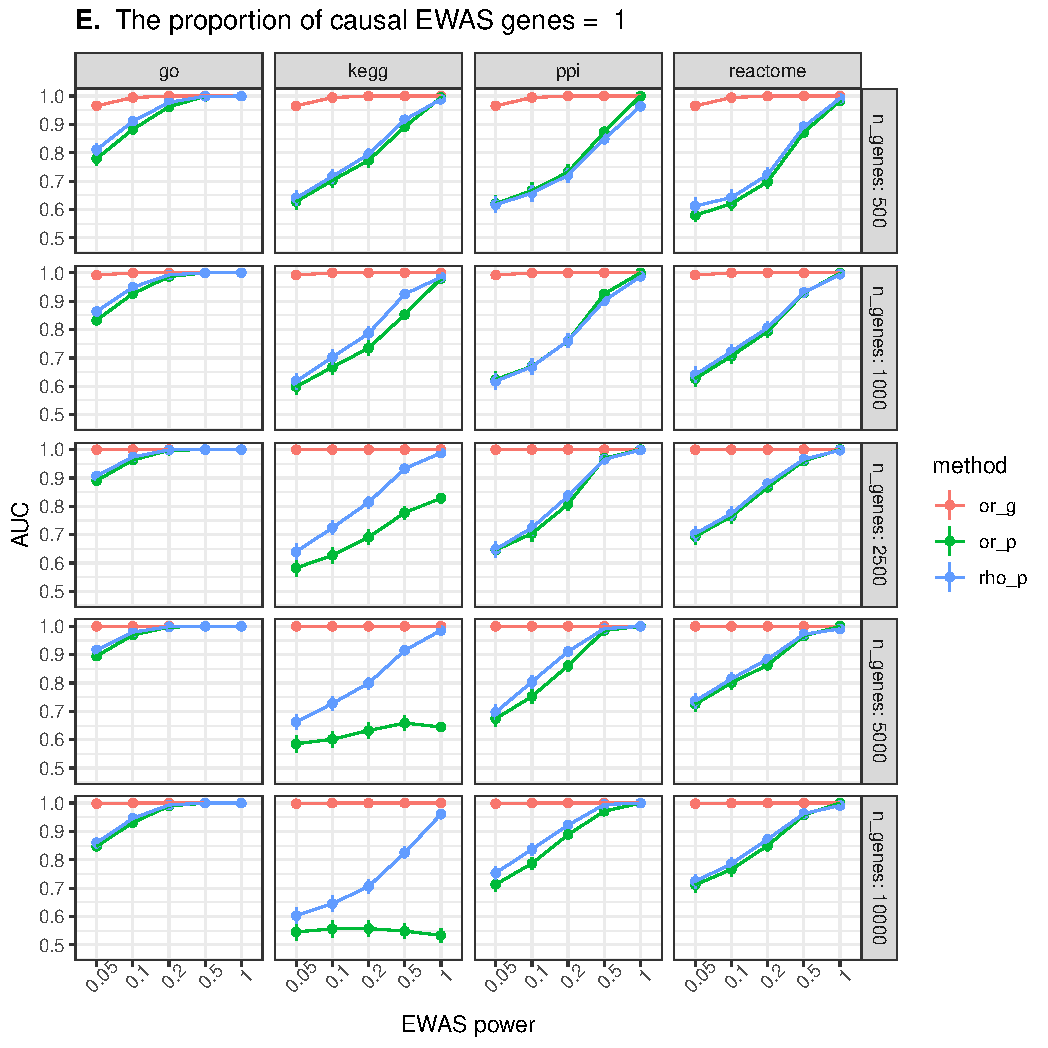
\includegraphics[width=1\linewidth]{figure/06-ewas_gwas_comparison/method_test_gene_up_all/PEC_1} 

}

\caption[Full results from simulations assessing power to detect overlap between genes and genesets identified by corresponding EWAS and GWAS]{\textbf{Full results from simulations assessing power to detect overlap between genes and genesets identified by corresponding EWAS and GWAS}. Simulations were set up as illustrated in \textbf{Figure \ref{fig:method-simulations-schematic}}. The ability to distinguish between results generated when EWAS and GWAS were sampling, in part, from the same set of causal genes and results generated when EWAS was sampling random genes from the genome. The header of each set indicates the proportion of genes identified by the simulated EWAS that were set to be causal. or\_g = assessing overlap of genes, or\_p = assessing overlap of genesets, rho\_p = assessing correlation between geneset enrichment scores. go = gene ontology, ppi = protein-protein interaction database from EpiGraphDB.}\label{fig:sim1-full-plot5}
\end{figure}



\begin{figure}

{\centering 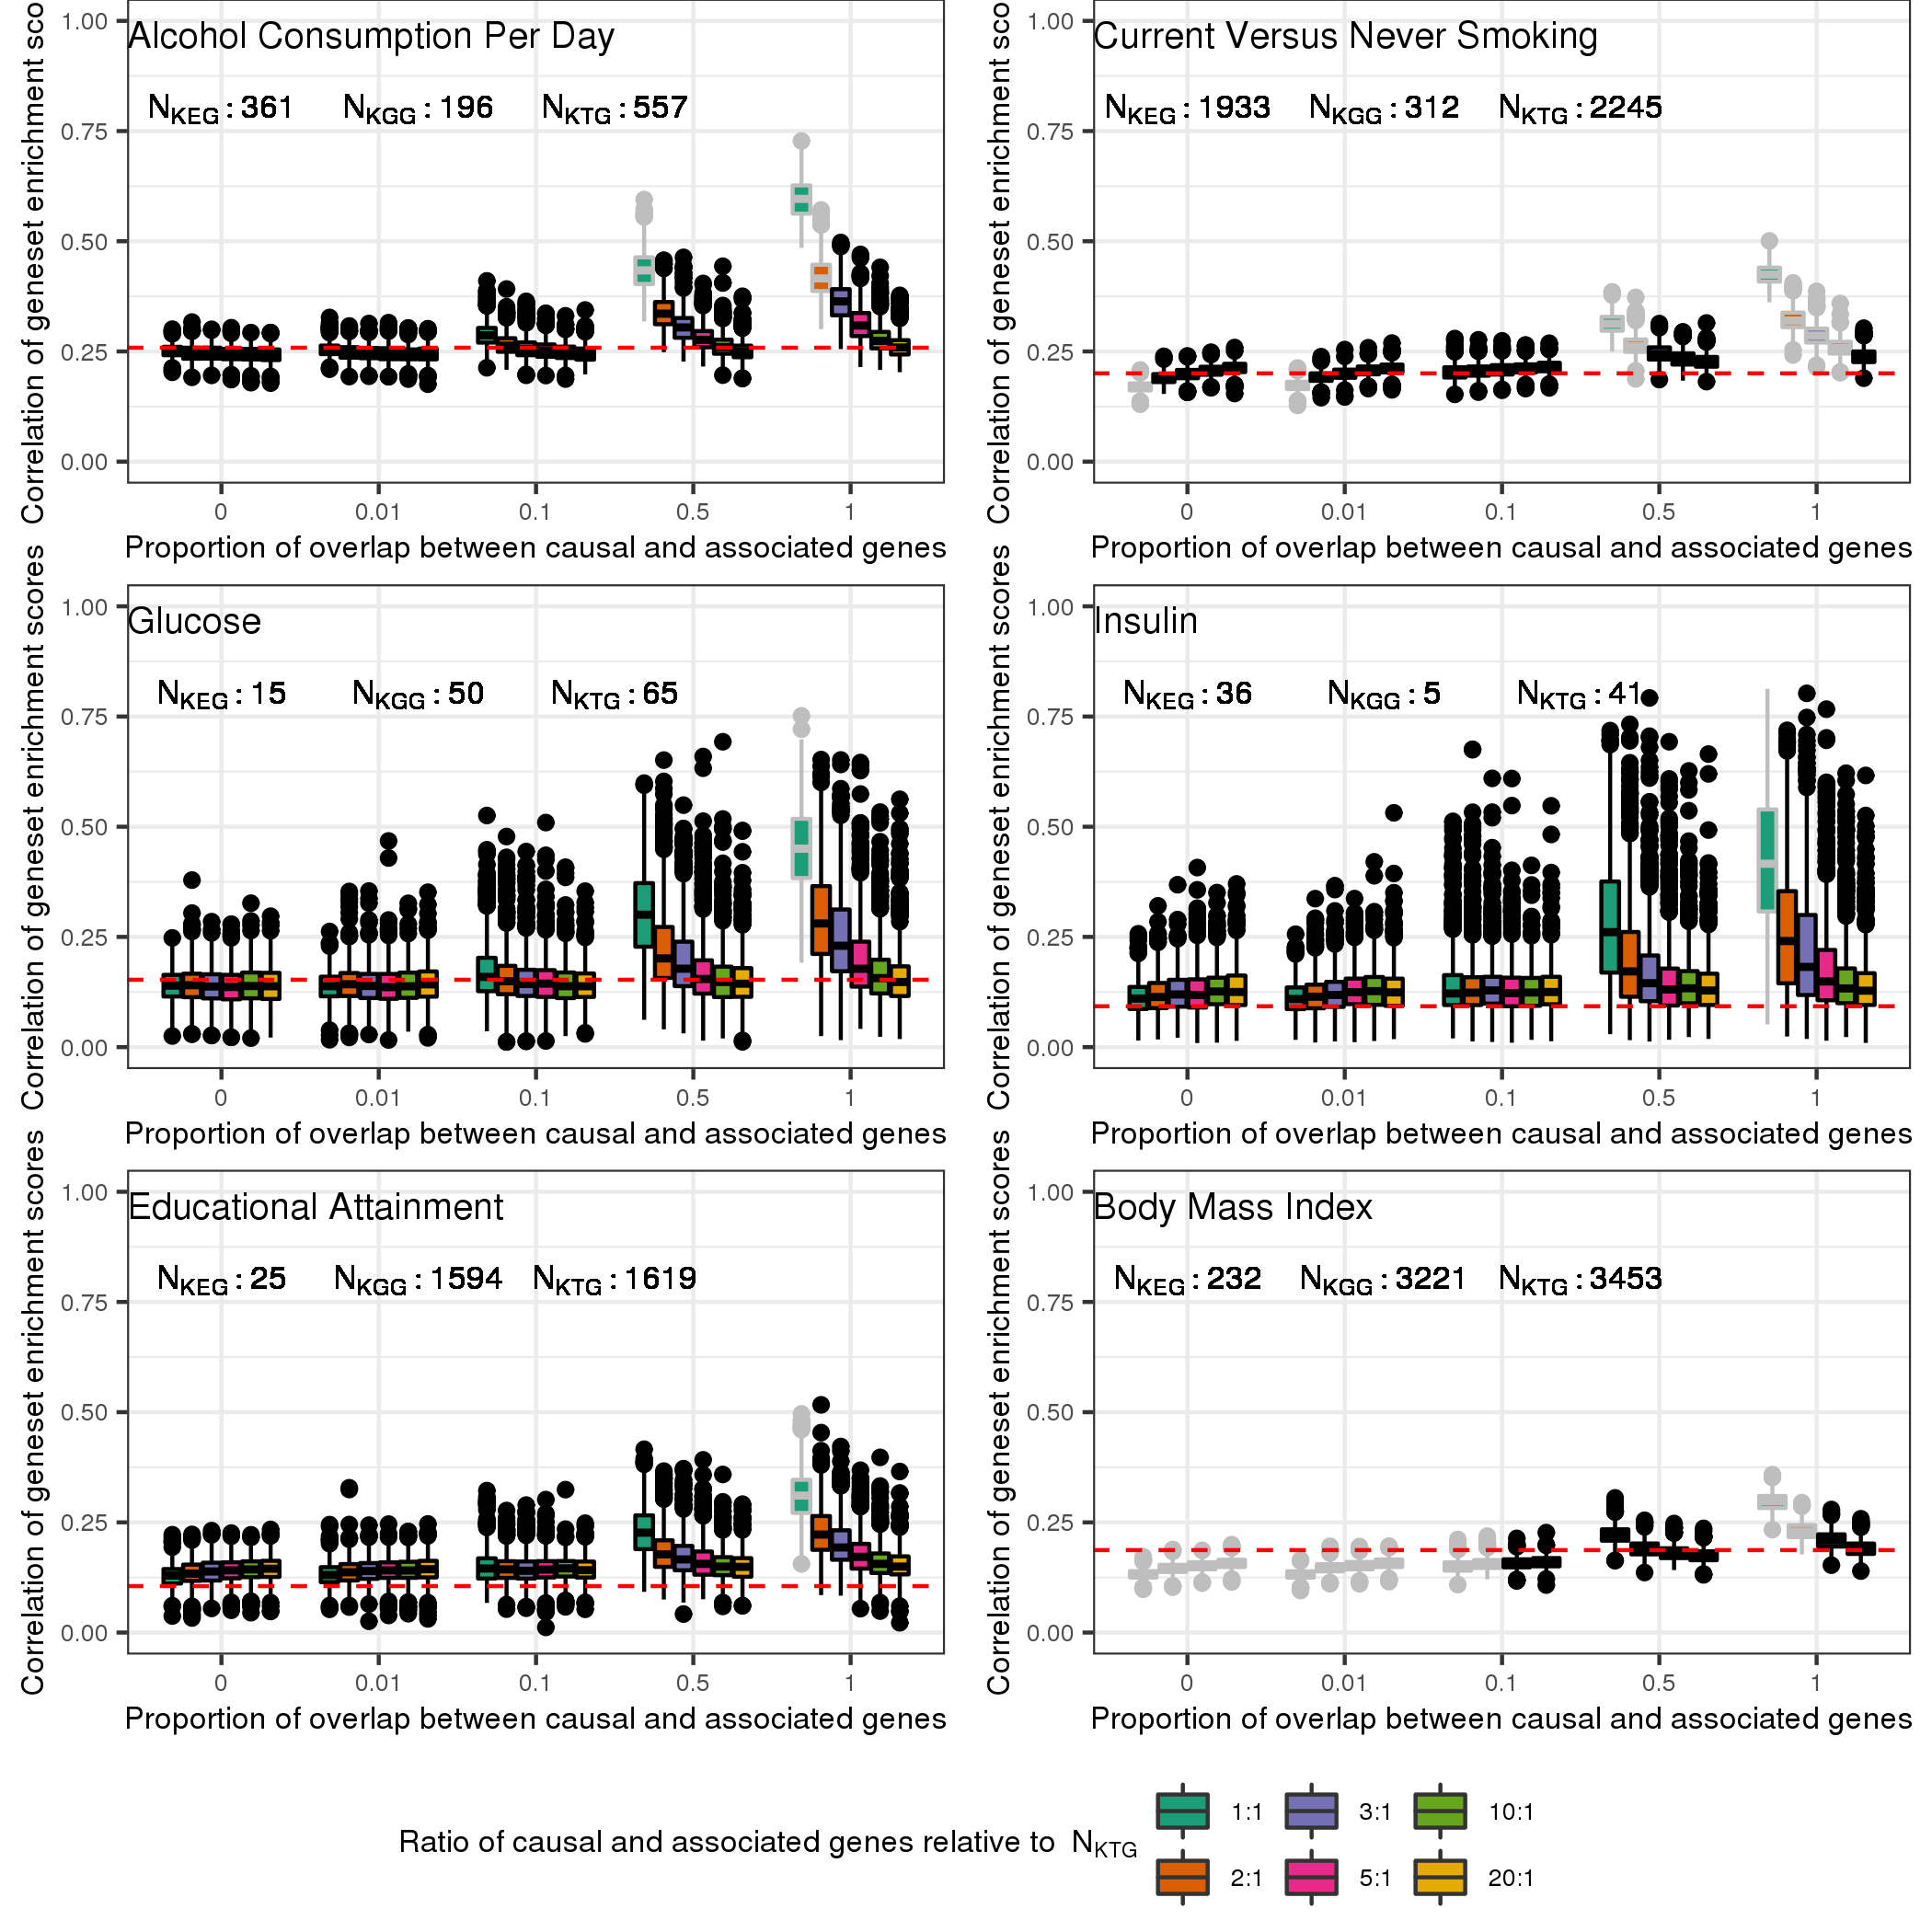
\includegraphics[width=1\linewidth]{figure/06-ewas_gwas_comparison/architecture_sims_other_traits_corr} 

}

\caption[Simulations to understand the likely number of genes still to identify in EWAS and GWAS of six traits under different trait architectures]{\textbf{Simulations to understand the likely number of genes still to identify in EWAS and GWAS of six traits under different trait architectures}. Simulations were set up as illustrated in \textbf{Figure \ref{fig:arch-simulations-schematic}}. Correlation of geneset enrichment scores from empirical data (\textbf{Table \ref{tab:empirical-pathway-tab}}), is shown as a red dashed line. Box plots show the range of enrichment score correlations from 1000 simulations using the parameters indicated. The number of causal and associated genes, as well as the overlap between these genes were varied. N\textsubscript{KEG} = number of known EWAS genes, N\textsubscript{KEG} = number of known GWAS genes, N\textsubscript{KTG} = number of known total genes (N\textsubscript{KEG} + N\textsubscript{KGG}). By way of an example, when N\textsubscript{KTG} = 557 and the ratio of causal and associated genes relative to N\textsubscript{KTG} is 1:1, the number of causal genes in the simulations will be 557 and the number of associated genes in the simulations will be 557. Scenarios which lie close to the empirical result (red dashed line) are more likely to reflect the true underlying number of genes related to a trait and the true overlap between the causal and associated genes.}\label{fig:arch-simulations-supp-res}
\end{figure}



\begin{center}\includegraphics[width=1\linewidth]{figure/06-ewas_gwas_comparison/method_test_gene_v_protein/PEC_0.05} \end{center}
\begin{center}\includegraphics[width=1\linewidth]{figure/06-ewas_gwas_comparison/method_test_gene_v_protein/PEC_0.1} \end{center}
\begin{center}\includegraphics[width=1\linewidth]{figure/06-ewas_gwas_comparison/method_test_gene_v_protein/PEC_0.2} \end{center}
\begin{center}\includegraphics[width=1\linewidth]{figure/06-ewas_gwas_comparison/method_test_gene_v_protein/PEC_0.5} \end{center}
\begin{figure}

{\centering \includegraphics[width=1\linewidth]{figure/06-ewas_gwas_comparison/method_test_gene_v_protein/PEC_1} 

}

\caption[Power to detect overlap between genes and genesets identified by corresponding EWAS and GWAS when mapping signal to all genes and protein coding genes]{\textbf{Power to detect overlap between genes and genesets identified by corresponding EWAS and GWAS when mapping signal to all genes and protein coding genes}. Simulations were set up as illustrated in \textbf{Figure \ref{fig:method-simulations-schematic}}. The ability to distinguish between results generated when EWAS and GWAS were sampling, in part, from the same set of causal genes and results generated when EWAS was sampling random genes from the genome. The header of each set indicates the proportion of genes identified by the simulated EWAS that were set to be causal. or\_g = assessing overlap of genes, or\_p = assessing overlap of genesets, rho\_p = assessing correlation between geneset enrichment scores. go = gene ontology, suffix of `-genes' denotes using all Ensembl gene IDs for the analysis and the suffix of `-proteins' denotes using only protein coding genes.}\label{fig:sim1-go-kegg-gene-comp5}
\end{figure}
\hypertarget{the-second-appendix-for-fun}{%
\chapter{The Second Appendix, for Fun}\label{the-second-appendix-for-fun}}

\backmatter

\hypertarget{references}{%
\chapter*{References}\label{references}}
\addcontentsline{toc}{chapter}{References}

\markboth{References}{References}

\noindent

\setlength{\parindent}{-0.20in}
\setlength{\leftskip}{0.20in}
\setlength{\parskip}{8pt}
\begin{center}\rule{0.5\linewidth}{0.5pt}\end{center}

\hypertarget{refs}{}
\begin{cslreferences}
\leavevmode\hypertarget{ref-Birney2016}{}%
1. Birney E, Smith GD, Greally JM. Epigenome-wide Association Studies and the Interpretation of Disease -Omics. \emph{PLOS Genetics} {[}electronic article{]}. 2016;12(6):e1006105. (\url{http://dx.plos.org/10.1371/journal.pgen.1006105})

\leavevmode\hypertarget{ref-Price2018}{}%
2. Price EM, Robinson WP. Adjusting for batch effects in DNA methylation microarray data, a lesson learned. \emph{Frontiers in Genetics}. 2018;

\leavevmode\hypertarget{ref-Gaunt2016}{}%
3. Gaunt TR, Shihab HA, Hemani G, et al. Systematic identification of genetic influences on methylation across the human life course. \emph{Genome Biology} {[}electronic article{]}. 2016;17(1):61. (\url{http://genomebiology.biomedcentral.com/articles/10.1186/s13059-016-0926-z})

\leavevmode\hypertarget{ref-Cobb2017}{}%
4. Cobb M. 60 years ago, Francis Crick changed the logic of biology. \emph{PLoS Biology}. 2017;

\leavevmode\hypertarget{ref-CRICK1958}{}%
5. CRICK FH. On protein synthesis. \emph{Symposia of the Society for Experimental Biology}. 1958;

\leavevmode\hypertarget{ref-Hafner2019}{}%
6. Hafner A, Bulyk ML, Jambhekar A, et al. The multiple mechanisms that regulate p53 activity and cell fate. 2019;

\leavevmode\hypertarget{ref-Corbett2018}{}%
7. Corbett AH. Post-transcriptional regulation of gene expression and human disease. 2018;

\leavevmode\hypertarget{ref-Wang2014}{}%
8. Wang YC, Peterson SE, Loring JF. Protein post-translational modifications and regulation of pluripotency in human stem cells. 2014;

\leavevmode\hypertarget{ref-Filipowicz2008}{}%
9. Filipowicz W, Bhattacharyya SN, Sonenberg N. Mechanisms of post-transcriptional regulation by microRNAs: Are the answers in sight? 2008;

\leavevmode\hypertarget{ref-Alberts2017}{}%
10. Alberts B, Johnson A, Lewis J, et al. Molecular Biology of the Cell. 2017.

\leavevmode\hypertarget{ref-Colby2011}{}%
11. Colby DW, Prusiner SB. Prions. \emph{Cold Spring Harbor Perspectives in Biology}. 2011;

\leavevmode\hypertarget{ref-Kornberg1999}{}%
12. Kornberg RD. Eukaryotic transcriptional control. 1999;

\leavevmode\hypertarget{ref-Gibney2010}{}%
13. Gibney ER, Nolan CM. Epigenetics and gene expression. 2010;

\leavevmode\hypertarget{ref-Milholland2017}{}%
14. Milholland B, Dong X, Zhang L, et al. Differences between germline and somatic mutation rates in humans and mice. \emph{Nature Communications}. 2017;

\leavevmode\hypertarget{ref-Suzuki2008}{}%
15. Suzuki MM, Bird A. DNA methylation landscapes: Provocative insights from epigenomics. 2008;

\leavevmode\hypertarget{ref-Siegfried1999}{}%
16. Siegfried Z, Eden S, Mendelsohn M, et al. DNA methylation represses transcription in vivo. \emph{Nature Genetics}. 1999;

\leavevmode\hypertarget{ref-Bird2002}{}%
17. Bird A. DNA methylation patterns and epigenetic memory. 2002;

\leavevmode\hypertarget{ref-Jones2012}{}%
18. Jones PA. Functions of DNA methylation: islands, start sites, gene bodies and beyond. \emph{Nature Reviews Genetics} {[}electronic article{]}. 2012;13(7):484--492. (\url{http://www.nature.com/articles/nrg3230})

\leavevmode\hypertarget{ref-Greally2018}{}%
19. Greally JM. A user's guide to the ambiguous word 'epigenetics'. 2018;

\leavevmode\hypertarget{ref-Stern2000}{}%
20. Stern CD. Conrad H. Waddington's contributions to avian and mammalian development, 1930-1940. \emph{International Journal of Developmental Biology}. 2000;

\leavevmode\hypertarget{ref-Bannister2011}{}%
21. Bannister AJ, Kouzarides T. Regulation of chromatin by histone modifications. 2011;

\leavevmode\hypertarget{ref-Berger2007}{}%
22. Berger SL. The complex language of chromatin regulation during transcription. 2007;

\leavevmode\hypertarget{ref-Jenuwein2001}{}%
23. Jenuwein T, Allis CD. Translating the histone code. 2001;

\leavevmode\hypertarget{ref-Kouzarides2007}{}%
24. Kouzarides T. Chromatin Modifications and Their Function. 2007;

\leavevmode\hypertarget{ref-Holliday1975}{}%
25. Holliday R, Pugh J. DNA modification mechanisms and gene activity during development. \emph{Science}. 1975;

\leavevmode\hypertarget{ref-Riggs1975}{}%
26. Riggs AD. X inactivation, differentiation, and DNA methylation. \emph{Cytogenetic and Genome Research}. 1975;

\leavevmode\hypertarget{ref-Bell2000}{}%
27. Bell AC, Felsenfeld G. Methylation of a CTCF-dependent boundary controls imprinted expression of the Igf2 gene. \emph{Nature}. 2000;

\leavevmode\hypertarget{ref-Yoder1997}{}%
28. Yoder JA, Walsh CP, Bestor TH. Cytosine methylation and the ecology of intragenomic parasites. 1997;

\leavevmode\hypertarget{ref-Casadesus2006}{}%
29. Casadesús J, Low D. Epigenetic Gene Regulation in the Bacterial World. \emph{Microbiology and Molecular Biology Reviews}. 2006;

\leavevmode\hypertarget{ref-Cokus2008}{}%
30. Cokus SJ, Feng S, Zhang X, et al. Shotgun bisulphite sequencing of the Arabidopsis genome reveals DNA methylation patterning. \emph{Nature}. 2008;

\leavevmode\hypertarget{ref-Rountree1997}{}%
31. Rountree MR, Selker EU. DNA methylation inhibits elongation but not initiation of transcription in Neurospora crassa. \emph{Genes and Development}. 1997;

\leavevmode\hypertarget{ref-Illingworth2009}{}%
32. Illingworth RS, Bird AP. CpG islands - 'A rough guide'. 2009;

\leavevmode\hypertarget{ref-Ando2019}{}%
33. Ando M, Saito Y, Xu G, et al. Chromatin dysregulation and DNA methylation at transcription start sites associated with transcriptional repression in cancers. \emph{Nature Communications}. 2019;

\leavevmode\hypertarget{ref-Deaton2011}{}%
34. Deaton AM, Bird A. CpG islands and the regulation of transcription. \emph{Genes and Development}. 2011;

\leavevmode\hypertarget{ref-Wolf1984}{}%
35. Wolf SF, Jolly DJ, Lunnen KD, et al. Methylation of the hypoxanthine phosphoribosyltransferase locus on the human X chromosome: Implications for X chromosome inactivation. \emph{Proceedings of the National Academy of Sciences of the United States of America}. 1984;

\leavevmode\hypertarget{ref-Hellman2007}{}%
36. Hellman A, Chess A. Gene body-specific methylation on the active X chromosome. \emph{Science}. 2007;

\leavevmode\hypertarget{ref-Zhu2016}{}%
37. Zhu H, Wang G, Qian J. Transcription factors as readers and effectors of DNA methylation. \emph{Nature Reviews Genetics}. 2016;

\leavevmode\hypertarget{ref-Jaffe2012}{}%
38. Jaffe AE, Murakami P, Lee H, et al. Bump hunting to identify differentially methylated regions in epigenetic epidemiology studies. \emph{International Journal of Epidemiology}. 2012;

\leavevmode\hypertarget{ref-Suderman2018}{}%
39. Suderman M, Staley JR, French R, et al. Dmrff: Identifying differentially methylated regions efficiently with power and control. \emph{bioRxiv}. 2018;

\leavevmode\hypertarget{ref-Challen2012}{}%
40. Challen GA, Sun D, Jeong M, et al. Dnmt3a is essential for hematopoietic stem cell differentiation. \emph{Nature Genetics}. 2012;

\leavevmode\hypertarget{ref-Lock1987}{}%
41. Lock LF, Takagi N, Martin GR. Methylation of the Hprt gene on the inactive X occurs after chromosome inactivation. \emph{Cell}. 1987;

\leavevmode\hypertarget{ref-Ohm2007}{}%
42. Ohm JE, McGarvey KM, Yu X, et al. A stem cell-like chromatin pattern may predispose tumor suppressor genes to DNA hypermethylation and heritable silencing. \emph{Nature Genetics}. 2007;

\leavevmode\hypertarget{ref-Prendergast1991}{}%
43. Prendergast GC, Ziff EB. Methylation-sensitive sequence-specific DNA binding by the c-Myc basic region. \emph{Science}. 1991;

\leavevmode\hypertarget{ref-Harrington1988}{}%
44. Harrington MA, Jones PA, Imagawa M, et al. Cytosine methylation does not affect binding of transcription factor Sp1. \emph{Proceedings of the National Academy of Sciences of the United States of America}. 1988;

\leavevmode\hypertarget{ref-Hemani2017}{}%
45. Hemani G, Tilling K, Davey Smith G. Orienting the causal relationship between imprecisely measured traits using GWAS summary data. \emph{PLoS Genetics}. 2017;

\leavevmode\hypertarget{ref-Wrzeska2004}{}%
46. Wrzeska M, Rejduch B. Genomic imprinting in mammals. 2004;

\leavevmode\hypertarget{ref-Nicholls2000}{}%
47. Nicholls RD. The impact of genomic imprinting for neurobehavioral and developmental disorders. 2000;

\leavevmode\hypertarget{ref-Lynch1998}{}%
48. Lynch M, Walsh B. Genetics and Analysis of Quantitative Traits. Sinauer; 1998.

\leavevmode\hypertarget{ref-Relton2010}{}%
49. Relton CL, Davey Smith G. Epigenetic Epidemiology of Common Complex Disease: Prospects for Prediction, Prevention, and Treatment. \emph{PLoS Medicine} {[}electronic article{]}. 2010;7(10):e1000356. (\url{http://dx.plos.org/10.1371/journal.pmed.1000356})

\leavevmode\hypertarget{ref-Weaver2004}{}%
50. Weaver ICG, Cervoni N, Champagne FA, et al. Epigenetic programming by maternal behavior. \emph{Nature Neuroscience}. 2004;

\leavevmode\hypertarget{ref-Koch2018}{}%
51. Koch A, Joosten SC, Feng Z, et al. Analysis of DNA methylation in cancer: Location revisited. 2018;

\leavevmode\hypertarget{ref-Hentze2019}{}%
52. Hentze J, Hødall C, Høgdall E. Methylation and ovarian cancer: Can DNA methylation be of diagnostic use? (Review). \emph{Molecular and Clinical Oncology}. 2019;

\leavevmode\hypertarget{ref-Cortellino2011}{}%
53. Cortellino S, Xu J, Sannai M, et al. Thymine DNA glycosylase is essential for active DNA demethylation by linked deamination-base excision repair. \emph{Cell}. 2011;

\leavevmode\hypertarget{ref-Kohli2013}{}%
54. Kohli RM, Zhang Y. TET enzymes, TDG and the dynamics of DNA demethylation. 2013;

\leavevmode\hypertarget{ref-Venolia1983}{}%
55. Venolia L, Gartler SM. Comparison of transformation efficiency of human active and inactive X-chromosomal DNA. 1983;

\leavevmode\hypertarget{ref-Bonasio2010}{}%
56. Bonasio R, Tu S, Reinberg D. Molecular signals of epigenetic states. 2010;

\leavevmode\hypertarget{ref-Allis2016}{}%
57. Allis CD, Jenuwein T. The molecular hallmarks of epigenetic control. \emph{Nat Rev Genet} {[}electronic article{]}. 2016;17(8):487--500. (\url{http://dx.doi.org/10.1038/nrg.2016.59\%20http://10.0.4.14/nrg.2016.59})

\leavevmode\hypertarget{ref-Wade2001}{}%
58. Wade PA, Wolffe AP. ReCoGnizing methylated DNA. 2001;

\leavevmode\hypertarget{ref-Ernst2015}{}%
59. Ernst J, Kellis M. Large-scale imputation of epigenomic datasets for systematic annotation of diverse human tissues. \emph{Nature Biotechnology}. 2015;

\leavevmode\hypertarget{ref-Shah2015}{}%
60. Shah S, Bonder MJ, Marioni RE, et al. Improving Phenotypic Prediction by Combining Genetic and Epigenetic Associations. \emph{American Journal of Human Genetics}. 2015;

\leavevmode\hypertarget{ref-Reed2020}{}%
61. Reed ZE, Suderman MJ, Relton CL, et al. The association of DNA methylation with body mass index: Distinguishing between predictors and biomarkers. \emph{Clinical Epigenetics}. 2020;

\leavevmode\hypertarget{ref-Yang2004}{}%
62. Yang AS. A simple method for estimating global DNA methylation using bisulfite PCR of repetitive DNA elements. \emph{Nucleic Acids Research}. 2004;

\leavevmode\hypertarget{ref-Dedeurwaerder2011}{}%
63. Dedeurwaerder S, Defrance M, Calonne E, et al. Evaluation of the Infinium Methylation 450K technology. \emph{Epigenomics}. 2011;

\leavevmode\hypertarget{ref-Lovkvist2016}{}%
64. Lövkvist C, Dodd IB, Sneppen K, et al. DNA methylation in human epigenomes depends on local topology of CpG sites. \emph{Nucleic Acids Research}. 2016;

\leavevmode\hypertarget{ref-Illumina2012}{}%
65. Illumina. Infinium HumanMethylation450 BeadChip The ideal solution for affordable, large sample--size genome-wide DNA methylation studies. 2012;4. (\url{https://emea.illumina.com/content/dam/illumina-marketing/documents/products/datasheets/datasheet\%7B/_\%7Dhumanmethylation450.pdf}). (Accessed August 5, 2020)

\leavevmode\hypertarget{ref-Rakyan2011}{}%
66. Rakyan VK, Down TA, Balding DJ, et al. Epigenome-wide association studies for common human diseases. \emph{Nature Reviews Genetics} {[}electronic article{]}. 2011;12(8):529--541. (\url{http://www.nature.com/articles/nrg3000})

\leavevmode\hypertarget{ref-Li2011}{}%
67. Li Y, Tollefsbol TO. DNA methylation detection: Bisulfite genomic sequencing analysis. \emph{Methods in Molecular Biology}. 2011;

\leavevmode\hypertarget{ref-Joehanes2016}{}%
68. Joehanes R, Just AC, Marioni RE, et al. Epigenetic Signatures of Cigarette Smoking. \emph{Circulation: Cardiovascular Genetics}. 2016;

\leavevmode\hypertarget{ref-Breitling2011}{}%
69. Breitling LP, Yang R, Korn B, et al. Tobacco-smoking-related differential DNA methylation: 27K discovery and replication. \emph{American Journal of Human Genetics}. 2011;

\leavevmode\hypertarget{ref-Wahl2017}{}%
70. Wahl S, Drong A, Lehne B, et al. Epigenome-wide association study of body mass index, and the adverse outcomes of adiposity. \emph{Nature} {[}electronic article{]}. 2017;541(7635):81--86. (\url{http://dx.doi.org/10.1038/nature20784})

\leavevmode\hypertarget{ref-Yang2013}{}%
71. Yang BZ, Zhang H, Ge W, et al. Child abuse and epigenetic mechanisms of disease risk. \emph{American Journal of Preventive Medicine}. 2013;

\leavevmode\hypertarget{ref-Felix2018}{}%
72. Felix JF, Joubert BR, Baccarelli AA, et al. Cohort profile: Pregnancy and childhood epigenetics (PACE) consortium. \emph{International Journal of Epidemiology}. 2018;

\leavevmode\hypertarget{ref-Philibert2016}{}%
73. Philibert R, Hollenbeck N, Andersen E, et al. Reversion of AHRR demethylation is a quantitative biomarker of smoking cessation. \emph{Frontiers in Psychiatry}. 2016;

\leavevmode\hypertarget{ref-Philibert2020}{}%
74. Philibert R, Dogan M, Beach SRH, et al. AHRR methylation predicts smoking status and smoking intensity in both saliva and blood DNA. \emph{American Journal of Medical Genetics, Part B: Neuropsychiatric Genetics}. 2020;

\leavevmode\hypertarget{ref-Horvath2013}{}%
75. Horvath S. DNA methylation age of human tissues and cell types. \emph{Genome Biology}. 2013;

\leavevmode\hypertarget{ref-Jones2015}{}%
76. Jones MJ, Goodman SJ, Kobor MS. DNA methylation and healthy human aging. 2015;

\leavevmode\hypertarget{ref-Horvath2018}{}%
77. Horvath S, Raj K. DNA methylation-based biomarkers and the epigenetic clock theory of ageing. 2018;

\leavevmode\hypertarget{ref-Houseman2012}{}%
78. Houseman EA, Accomando WP, Koestler DC, et al. DNA methylation arrays as surrogate measures of cell mixture distribution. \emph{BMC Bioinformatics}. 2012;

\leavevmode\hypertarget{ref-Jaffe2014}{}%
79. Jaffe AE, Irizarry RA. Accounting for cellular heterogeneity is critical in epigenome-wide association studies. \emph{Genome Biology}. 2014;

\leavevmode\hypertarget{ref-McGregor2016}{}%
80. McGregor K, Bernatsky S, Colmegna I, et al. An evaluation of methods correcting for cell-type heterogeneity in DNA methylation studies. \emph{Genome Biology}. 2016;

\leavevmode\hypertarget{ref-Teschendorff2017}{}%
81. Teschendorff AE, Zheng SC. Cell-type deconvolution in epigenome-wide association studies: A review and recommendations. 2017;

\leavevmode\hypertarget{ref-Forest2018}{}%
82. Forest M, O'Donnell KJ, Voisin G, et al. Agreement in DNA methylation levels from the Illumina 450K array across batches, tissues, and time. \emph{Epigenetics}. 2018;

\leavevmode\hypertarget{ref-Zhou2017}{}%
83. Zhou W, Laird PW, Shen H. Comprehensive characterization, annotation and innovative use of Infinium DNA methylation BeadChip probes. \emph{Nucleic acids research}. 2017;

\leavevmode\hypertarget{ref-Naeem2014}{}%
84. Naeem H, Wong NC, Chatterton Z, et al. Reducing the risk of false discovery enabling identification of biologically significant genome-wide methylation status using the HumanMethylation450 array. \emph{BMC Genomics}. 2014;

\leavevmode\hypertarget{ref-Leek2007}{}%
85. Leek JT, Storey JD. Capturing heterogeneity in gene expression studies by surrogate variable analysis. \emph{PLoS Genetics}. 2007;

\leavevmode\hypertarget{ref-Ritchie2015}{}%
86. Ritchie ME, Phipson B, Wu D, et al. Limma powers differential expression analyses for RNA-sequencing and microarray studies. \emph{Nucleic Acids Research}. 2015;

\leavevmode\hypertarget{ref-Perrier2018}{}%
87. Perrier F, Novoloaca A, Ambatipudi S, et al. Identifying and correcting epigenetics measurements for systematic sources of variation. \emph{Clinical Epigenetics}. 2018;

\leavevmode\hypertarget{ref-Piekarz2009}{}%
88. Piekarz RL, Bates SE. Epigenetic modifiers: Basic understanding and clinical development. 2009;

\leavevmode\hypertarget{ref-Nebbioso2018}{}%
89. Nebbioso A, Tambaro FP, Dell'Aversana C, et al. Cancer epigenetics: Moving forward. 2018;

\leavevmode\hypertarget{ref-Pickar-Oliver2019}{}%
90. Pickar-Oliver A, Gersbach CA. The next generation of CRISPR--Cas technologies and applications. 2019;

\leavevmode\hypertarget{ref-Liao2017}{}%
91. Liao HK, Hatanaka F, Araoka T, et al. In Vivo Target Gene Activation via CRISPR/Cas9-Mediated Trans-epigenetic Modulation. \emph{Cell}. 2017;

\leavevmode\hypertarget{ref-DaveySmith2003}{}%
92. Davey Smith G, Ebrahim S. 'Mendelian randomization': Can genetic epidemiology contribute to understanding environmental determinants of disease? 2003;

\leavevmode\hypertarget{ref-DaveySmith2014}{}%
93. Davey Smith G, Hemani G. Mendelian randomization: genetic anchors for causal inference in epidemiological studies. \emph{Human molecular genetics} {[}electronic article{]}. 2014;23(R1):R89--98. (\url{http://hmg.oxfordjournals.org/cgi/content/long/23/R1/R89})

\leavevmode\hypertarget{ref-Buniello2019}{}%
94. Buniello A, Macarthur JAL, Cerezo M, et al. The NHGRI-EBI GWAS Catalog of published genome-wide association studies, targeted arrays and summary statistics 2019. \emph{Nucleic Acids Research}. 2019;

\leavevmode\hypertarget{ref-Elsworth2020}{}%
95. Elsworth\hspace{0pt} B, Lyon\hspace{0pt} M, Alexander\hspace{0pt} T, et al. The MRC IEU OpenGWAS data infrastructure. \emph{bioRxiv}. 2020;

\leavevmode\hypertarget{ref-Hemani2018}{}%
96. Hemani G, Zheng J, Elsworth B, et al. The MR-base platform supports systematic causal inference across the human phenome. \emph{eLife}. 2018;

\leavevmode\hypertarget{ref-Liu2019}{}%
97. Liu D, Zhao L, Wang Z, et al. EWASdb: Epigenome-wide association study database. \emph{Nucleic Acids Research}. 2019;

\leavevmode\hypertarget{ref-Li2019}{}%
98. Li M, Zou D, Li Z, et al. EWAS Atlas: A curated knowledgebase of epigenome-wide association studies. \emph{Nucleic Acids Research}. 2019;

\leavevmode\hypertarget{ref-Yang2010}{}%
99. Yang J, Benyamin B, McEvoy BP, et al. Common SNPs explain a large proportion of the heritability for human height. \emph{Nature Genetics}. 2010;

\leavevmode\hypertarget{ref-Speed2012}{}%
100. Speed D, Hemani G, Johnson MR, et al. Improved heritability estimation from genome-wide SNPs. \emph{American Journal of Human Genetics}. 2012;

\leavevmode\hypertarget{ref-Phipson2016}{}%
101. Phipson B, Maksimovic J, Oshlack A. MissMethyl: An R package for analyzing data from Illumina's HumanMethylation450 platform. \emph{Bioinformatics}. 2016;

\leavevmode\hypertarget{ref-Philibert2012}{}%
102. Philibert RA, Beach SRH, Brody GH. Demethylation of the aryl hydrocarbon receptor repressor as a biomarker for nascent smokers. \emph{Epigenetics}. 2012;

\leavevmode\hypertarget{ref-Shenker2013}{}%
103. Shenker NS, Polidoro S, Veldhoven K van, et al. Epigenome-wide association study in the European Prospective Investigation Into Cancer And Nutrition (EPIC-Turin) identifies novel genetic loci associated with smoking. \emph{Human Molecular Genetics}. 2013;

\leavevmode\hypertarget{ref-Zeilinger2013}{}%
104. Zeilinger S, Kühnel B, Klopp N, et al. Tobacco Smoking Leads to Extensive Genome-Wide Changes in DNA Methylation. \emph{PLoS ONE}. 2013;

\leavevmode\hypertarget{ref-Bojesen2017}{}%
105. Bojesen SE, Timpson N, Relton C, et al. AHRR (cg05575921) hypomethylation marks smoking behaviour, morbidity and mortality. \emph{Thorax}. 2017;

\leavevmode\hypertarget{ref-Haarmann-Stemmann2006}{}%
106. Haarmann-Stemmann T, Abel J. The arylhydrocarbon receptor repressor (AhRR): Structure, expression, and function. 2006;

\leavevmode\hypertarget{ref-Larigot2018}{}%
107. Larigot L, Juricek L, Dairou J, et al. AhR signaling pathways and regulatory functions. 2018;

\leavevmode\hypertarget{ref-Richmond2016}{}%
108. Richmond RC, Hemani G, Tilling K, et al. Challenges and novel approaches for investigating molecular mediation. \emph{Human molecular genetics} {[}electronic article{]}. 2016;ddw197. (\url{http://hmg.oxfordjournals.org/cgi/content/long/ddw197v2})

\leavevmode\hypertarget{ref-Silventoinen2003}{}%
109. Silventoinen K, Kaprio J, Lahelma E, et al. Assortative mating by body height and BMI: Finnish twins and their spouses. \emph{American Journal of Human Biology}. 2003;

\leavevmode\hypertarget{ref-Maes1997}{}%
110. Maes HHM, Neale MC, Eaves LJ. Genetic and environmental factors in relative body weight and human adiposity. 1997;

\leavevmode\hypertarget{ref-Eaves1981}{}%
111. Eaves LJ, Heath AC. Detection of the effects of asymmetric assortative mating. \emph{Nature}. 1981;

\leavevmode\hypertarget{ref-Howe2019}{}%
112. Howe LJ, Lawson DJ, Davies NM, et al. Genetic evidence for assortative mating on alcohol consumption in the UK Biobank. \emph{Nature Communications}. 2019;

\leavevmode\hypertarget{ref-Dugue2019}{}%
113. Dugué PA, Wilson R, Lehne B, et al. Alcohol consumption is associated with widespread changes in blood DNA methylation: Analysis of cross-sectional and longitudinal data. \emph{Addiction Biology}. 2019;

\leavevmode\hypertarget{ref-Inoue2010}{}%
114. Inoue A, Solon G. Two-Sample Instrumental variables estimators. \emph{The Review of Economics and Statistics}. 2010;92(3):557--561.

\leavevmode\hypertarget{ref-Pierce2013}{}%
115. Pierce BL, Burgess S. Efficient design for mendelian randomization studies: Subsample and 2-sample instrumental variable estimators. \emph{American Journal of Epidemiology}. 2013;178(7):1177--1184.

\leavevmode\hypertarget{ref-Relton2012}{}%
116. Relton CL, Davey Smith G. Two-step epigenetic mendelian randomization: A strategy for establishing the causal role of epigenetic processes in pathways to disease. \emph{International Journal of Epidemiology}. 2012;

\leavevmode\hypertarget{ref-Richardson2018}{}%
117. Richardson TG, Haycock PC, Zheng J, et al. Systematic Mendelian randomization framework elucidates hundreds of CpG sites which may mediate the influence of genetic variants on disease. \emph{Human Molecular Genetics}. 2018;

\leavevmode\hypertarget{ref-Neumeyer2020}{}%
118. Neumeyer S, Hemani G, Zeggini E. Strengthening Causal Inference for Complex Disease Using Molecular Quantitative Trait Loci. 2020;

\leavevmode\hypertarget{ref-Johnston2019}{}%
119. Johnston AD, Simões-Pires CA, Thompson TV, et al. Functional genetic variants can mediate their regulatory effects through alteration of transcription factor binding. \emph{Nature Communications}. 2019;

\leavevmode\hypertarget{ref-Bonder2017}{}%
120. Bonder MJ, Luijk R, Zhernakova DV, et al. Disease variants alter transcription factor levels and methylation of their binding sites. \emph{Nature Genetics}. 2017;

\leavevmode\hypertarget{ref-Lawlor2016}{}%
121. Lawlor DA, Tilling K, Smith GD. Triangulation in aetiological epidemiology. \emph{International Journal of Epidemiology}. 2016;

\leavevmode\hypertarget{ref-Pearl2010}{}%
122. Pearl J. An introduction to causal inference. 2010;

\leavevmode\hypertarget{ref-Hernan2016}{}%
123. Hernán MA, Robins JM. Using Big Data to Emulate a Target Trial When a Randomized Trial Is Not Available. \emph{American Journal of Epidemiology}. 2016;

\leavevmode\hypertarget{ref-Hernan2018}{}%
124. Hernán MA. How to estimate the effect of treatment duration on survival outcomes using observational data. \emph{BMJ (Clinical research ed.)}. 2018;

\leavevmode\hypertarget{ref-Baglietto2017}{}%
125. Baglietto L, Ponzi E, Haycock P, et al. DNA methylation changes measured in pre-diagnostic peripheral blood samples are associated with smoking and lung cancer risk. \emph{International Journal of Cancer}. 2017;140(1):50--61.

\leavevmode\hypertarget{ref-Fraser2013}{}%
126. Fraser A, Macdonald-wallis C, Tilling K, et al. Cohort profile: The avon longitudinal study of parents and children: ALSPAC mothers cohort. \emph{International Journal of Epidemiology}. 2013;

\leavevmode\hypertarget{ref-Boyd2013}{}%
127. Boyd A, Golding J, Macleod J, et al. Cohort profile: The 'Children of the 90s'-The index offspring of the avon longitudinal study of parents and children. \emph{International Journal of Epidemiology}. 2013;42(1):111--127.

\leavevmode\hypertarget{ref-Harris2009}{}%
128. Harris PA, Taylor R, Thielke R, et al. Research electronic data capture (REDCap)-A metadata-driven methodology and workflow process for providing translational research informatics support. \emph{Journal of Biomedical Informatics}. 2009;

\leavevmode\hypertarget{ref-Harris2019}{}%
129. Harris PA, Taylor R, Minor BL, et al. The REDCap consortium: Building an international community of software platform partners. 2019;

\leavevmode\hypertarget{ref-McKay2017}{}%
130. McKay JD, Hung RJ, Han Y, et al. Large-scale association analysis identifies new lung cancer susceptibility loci and heterogeneity in genetic susceptibility across histological subtypes. \emph{Nature genetics} {[}electronic article{]}. 2017;49(7):1126--1132. (\url{http://www.nature.com/doifinder/10.1038/ng.3892\%7B/\%\%7D5Cnhttp://www.ncbi.nlm.nih.gov/pubmed/28604730})

\leavevmode\hypertarget{ref-Logue2017}{}%
131. Logue MW, Smith AK, Wolf EJ, et al. The correlation of methylation levels measured using Illumina 450K and EPIC BeadChips in blood samples. \emph{Epigenomics}. 2017;

\leavevmode\hypertarget{ref-IlluminaEPIC}{}%
132. Illumina. Infinium MethylationEPIC BeadChip - Datasheet. (\url{https://science-docs.illumina.com/documents/Microarray/infinium-methylation-epic-data-sheet-1070-2015-008/Content/Source/Microarray/Infinium/MethylationEPIC/infinium-methylation-epic-data-sheet.html})

\leavevmode\hypertarget{ref-Huang2015}{}%
133. Huang WY, Hsu SD, Huang HY, et al. MethHC: A database of DNA methylation and gene expression in human cancer. \emph{Nucleic Acids Research}. 2015;

\leavevmode\hypertarget{ref-Relton2015-aries}{}%
134. Relton CL, Gaunt T, McArdle W, et al. Data Resource Profile: Accessible Resource for Integrated Epigenomic Studies (ARIES). \emph{International Journal of Epidemiology} {[}electronic article{]}. 2015;44(4):1181--1190. (\url{http://dx.doi.org/10.1093/ije/dyv072})

\leavevmode\hypertarget{ref-Chen2017}{}%
135. Chen J, Behnam E, Huang J, et al. Fast and robust adjustment of cell mixtures in epigenome-wide association studies with SmartSVA. \emph{BMC Genomics}. 2017;

\leavevmode\hypertarget{ref-Nano2017}{}%
136. Nano J, Ghanbari M, Wang W, et al. Epigenome-Wide Association Study Identifies Methylation Sites Associated With Liver Enzymes and Hepatic Steatosis. \emph{Gastroenterology}. 2017;

\leavevmode\hypertarget{ref-Kaushal2017}{}%
137. Kaushal A, Zhang H, Karmaus WJJ, et al. Genome-wide DNA methylation at birth in relation to in utero arsenic exposure and the associated health in later life. \emph{Environmental Health: A Global Access Science Source}. 2017;

\leavevmode\hypertarget{ref-Morris2017}{}%
138. Morris JA, Tsai PC, Joehanes R, et al. Epigenome-wide Association of DNA Methylation in Whole Blood With Bone Mineral Density. \emph{Journal of Bone and Mineral Research}. 2017;

\leavevmode\hypertarget{ref-Hedman2017}{}%
139. Hedman ÅK, Mendelson MM, Marioni RE, et al. Epigenetic Patterns in Blood Associated with Lipid Traits Predict Incident Coronary Heart Disease Events and Are Enriched for Results from Genome-Wide Association Studies. \emph{Circulation: Cardiovascular Genetics}. 2017;

\leavevmode\hypertarget{ref-Braun2017}{}%
140. Braun KVE, Dhana K, Vries PS de, et al. Epigenome-wide association study (EWAS) on lipids: the Rotterdam Study. \emph{Clinical Epigenetics}. 2017;

\leavevmode\hypertarget{ref-Teschendorff2015}{}%
141. Teschendorff AE, Yang Z, Wong A, et al. Correlation of Smoking-Associated DNA Methylation Changes in Buccal Cells With DNA Methylation Changes in Epithelial Cancer. \emph{JAMA oncology} {[}electronic article{]}. 2015;1(4):476--85. (\url{http://oncology.jamanetwork.com/article.aspx?articleid=2293216})

\leavevmode\hypertarget{ref-Corbin2019}{}%
142. Corbin LJ, Taylor AE, White SJ, et al. Epigenetic regulation of PAR4-related platelet activation: mechanistic links between environmental exposure and cardiovascular disease. \emph{bioRxiv} {[}electronic article{]}. 2019;473728. (\url{http://biorxiv.org/content/early/2019/01/03/473728.abstract})

\leavevmode\hypertarget{ref-Elliott2014}{}%
143. Elliott HR, Tillin T, McArdle WL, et al. Differences in smoking associated DNA methylation patterns in South Asians and Europeans. \emph{Clinical Epigenetics}. 2014;

\leavevmode\hypertarget{ref-Zudaire2008}{}%
144. Zudaire E, Cuesta N, Murty V, et al. The aryl hydrocarbon receptor repressor is a putative tumor suppressor gene in multiple human cancers. \emph{The Journal of clinical investigation}. 2008;

\leavevmode\hypertarget{ref-McRae2014}{}%
145. McRae AF, Powell JE, Henders AK, et al. Contribution of genetic variation to transgenerational inheritance of DNA methylation. \emph{Genome biology}. 2014;

\leavevmode\hypertarget{ref-Hannon2018}{}%
146. Hannon E, Knox O, Sugden K, et al. Characterizing genetic and environmental influences on variable DNA methylation using monozygotic and dizygotic twins. \emph{PLoS Genetics}. 2018;

\leavevmode\hypertarget{ref-Garg2018}{}%
147. Garg P, Joshi RS, Watson C, et al. A survey of inter-individual variation in DNA methylation identifies environmentally responsive co-regulated networks of epigenetic variation in the human genome. \emph{PLoS Genetics}. 2018;

\leavevmode\hypertarget{ref-Meng2010}{}%
148. Meng H, Joyce AR, Adkins DE, et al. A statistical method for excluding non-variable CpG sites in high-throughput DNA methylation profiling. \emph{BMC Bioinformatics}. 2010;

\leavevmode\hypertarget{ref-Min2018}{}%
149. Min JL, Hemani G, Davey Smith G, et al. Meffil: efficient normalization and analysis of very large DNA methylation datasets. \emph{Bioinformatics (Oxford, England)}. 2018;

\leavevmode\hypertarget{ref-Min2020}{}%
150. Min JL, Hemani G, Hannon E, et al. Genomic and phenomic insights from an atlas of genetic effects on DNA methylation. \emph{medRxiv} {[}electronic article{]}. 2020;2020.09.01.20180406. (\url{http://medrxiv.org/content/early/2020/09/03/2020.09.01.20180406.abstract})

\leavevmode\hypertarget{ref-VanDongen2016}{}%
151. Dongen J van, Nivard MG, Willemsen G, et al. Genetic and environmental influences interact with age and sex in shaping the human methylome. \emph{Nature Communications} {[}electronic article{]}. 2016;7:11115. (\url{http://www.nature.com/doifinder/10.1038/ncomms11115})

\leavevmode\hypertarget{ref-Sheffield2016}{}%
152. Sheffield NC, Bock C. LOLA: Enrichment analysis for genomic region sets and regulatory elements in R and Bioconductor. \emph{Bioinformatics}. 2016;

\leavevmode\hypertarget{ref-Kundaje2015}{}%
153. Kundaje A, Meuleman W, Ernst J, et al. Integrative analysis of 111 reference human epigenomes. \emph{Nature} {[}electronic article{]}. 2015;518(7539):317--330. (\url{http://www.nature.com/doifinder/10.1038/nature14248})

\leavevmode\hypertarget{ref-Dunham2012}{}%
154. Dunham I, Kundaje A, Aldred SF, et al. An integrated encyclopedia of DNA elements in the human genome. \emph{Nature}. 2012;

\leavevmode\hypertarget{ref-Mendelson2017}{}%
155. Mendelson MM, Marioni RE, Joehanes R, et al. Association of Body Mass Index with DNA Methylation and Gene Expression in Blood Cells and Relations to Cardiometabolic Disease: A Mendelian Randomization Approach. \emph{PLoS Medicine}. 2017;

\leavevmode\hypertarget{ref-Demerath2015}{}%
156. Demerath EW, Guan W, Grove ML, et al. Epigenome-wide association study (EWAS) of BMI, BMI change and waist circumference in African American adults identifies multiple replicated loci. \emph{Human molecular genetics}. 2015;

\leavevmode\hypertarget{ref-Sayols-Baixeras2016}{}%
157. Sayols-Baixeras S, Subirana I, Lluis-Ganella C, et al. Identification and validation of seven new loci showing differential DNA methylation related to serum lipid profile: An epigenome-wide approach. The REGICOR study. \emph{Human Molecular Genetics}. 2016;

\leavevmode\hypertarget{ref-Kriebel2016}{}%
158. Kriebel J, Herder C, Rathmann W, et al. Association between DNA Methylation in whole blood and measures of glucose metabolism: Kora F4 study. \emph{PLoS ONE}. 2016;

\leavevmode\hypertarget{ref-Pfeiffer2015}{}%
159. Pfeiffer L, Wahl S, Pilling LC, et al. DNA Methylation of Lipid-Related Genes Affects Blood Lipid Levels. \emph{Circulation: Cardiovascular Genetics}. 2015;

\leavevmode\hypertarget{ref-Chambers2015}{}%
160. Chambers JC, Loh M, Lehne B, et al. Epigenome-wide association of DNA methylation markers in peripheral blood from Indian Asians and Europeans with incident type 2 diabetes: A nested case-control study. \emph{The Lancet Diabetes and Endocrinology}. 2015;

\leavevmode\hypertarget{ref-Pidsley2016}{}%
161. Pidsley R, Zotenko E, Peters TJ, et al. Critical evaluation of the Illumina MethylationEPIC BeadChip microarray for whole-genome DNA methylation profiling. \emph{Genome Biology}. 2016;

\leavevmode\hypertarget{ref-ToinetCronje2020}{}%
162. Toinét Cronjé H, Elliott HR, Nienaber-Rousseau C, et al. Replication and expansion of epigenome-wide association literature in a black South African population. \emph{Clinical Epigenetics}. 2020;

\leavevmode\hypertarget{ref-Jones2009}{}%
163. Jones P a, Liang G. Rethinking how DNA methylation patterns are maintained. \emph{Nature reviews. Genetics} {[}electronic article{]}. 2009;10(11):805--11. (\url{http://www.pubmedcentral.nih.gov/articlerender.fcgi?artid=2848124\%7B/\&\%7Dtool=pmcentrez\%7B/\&\%7Drendertype=abstract\%7B/\%\%7D5Cnhttp://www.ncbi.nlm.nih.gov/entrez/query.fcgi?cmd=Retrieve\%7B/\&\%7Ddb=PubMed\%7B/\&\%7Ddopt=Citation\%7B/\&\%7Dlist\%7B/_\%7Duids=19789556})

\leavevmode\hypertarget{ref-Chen2016}{}%
164. Chen DP, Lin YC, Fann CSJ. Methods for identifying differentially methylated regions for sequence- and array-based data. \emph{Briefings in Functional Genomics}. 2016;15(6):485--490.

\leavevmode\hypertarget{ref-Lettre2008}{}%
165. Lettre G, Jackson AU, Gieger C, et al. Identification of ten loci associated with height highlights new biological pathways in human growth. \emph{Nature Genetics}. 2008;

\leavevmode\hypertarget{ref-Frayling2007}{}%
166. Frayling TM, Timpson NJ, Weedon MN, et al. A common variant in the FTO gene is associated with body mass index and predisposes to childhood and adult obesity. \emph{Science}. 2007;

\leavevmode\hypertarget{ref-Yengo2018}{}%
167. Yengo L, Sidorenko J, Kemper KE, et al. Meta-analysis of genome-wide association studies for height and body mass index in \textasciitilde700 000 individuals of European ancestry. \emph{Human Molecular Genetics}. 2018;

\leavevmode\hypertarget{ref-Dick2014}{}%
168. Dick KJ, Nelson CP, Tsaprouni L, et al. DNA methylation and body-mass index: A genome-wide analysis. \emph{The Lancet}. 2014;

\leavevmode\hypertarget{ref-Tahara2015}{}%
169. Tahara T, Arisawa T. DNA methylation as a molecular biomarker in gastric cancer. \emph{Epigenomics} {[}electronic article{]}. 2015;7(3):475--486. (\url{http://www.scopus.com/inward/record.url?eid=2-s2.0-84931360022\%7B/\&\%7DpartnerID=40\%7B/\&\%7Dmd5=96d2e2dd124d468e02c3b2da40e66212})

\leavevmode\hypertarget{ref-Kandimalla2013}{}%
170. Kandimalla R, Tilborg AA van, Zwarthoff EC. DNA methylation-based biomarkers in bladder cancer. \emph{Nature Reviews Urology} {[}electronic article{]}. 2013;10(6):327--335. (\url{http://www.nature.com/articles/nrurol.2013.89})

\leavevmode\hypertarget{ref-Speed2017}{}%
171. Speed D, Cai N, Johnson MR, et al. Reevaluation of SNP heritability in complex human traits. \emph{Nature Genetics} {[}electronic article{]}. 2017;49(7):986--992. (\url{http://www.nature.com/doifinder/10.1038/ng.3865})

\leavevmode\hypertarget{ref-Yang2011}{}%
172. Yang J, Lee SH, Goddard ME, et al. GCTA: A tool for genome-wide complex trait analysis. \emph{American Journal of Human Genetics} {[}electronic article{]}. 2011;88(1):76--82. (\url{http://arxiv.org/abs/NIHMS150003})

\leavevmode\hypertarget{ref-Chang2015}{}%
173. Chang CC, Chow CC, Tellier LC, et al. Second-generation PLINK: rising to the challenge of larger and richer datasets. \emph{GigaScience} {[}electronic article{]}. 2015;4(1):7. (\url{https://academic.oup.com/gigascience/article-lookup/doi/10.1186/s13742-015-0047-8})

\leavevmode\hypertarget{ref-Gazal2017}{}%
174. Gazal S, Finucane HK, Furlotte NA, et al. Linkage disequilibrium--dependent architecture of human complex traits shows action of negative selection. \emph{Nature Genetics} {[}electronic article{]}. 2017;49(10):1421--1427. (\url{http://www.nature.com/doifinder/10.1038/ng.3954})

\leavevmode\hypertarget{ref-Speed2018}{}%
175. Speed D, Balding D. Exposing flaws in S-LDSC; reply to Gazal et al. \emph{bioRxiv} {[}electronic article{]}. 2018;280784. (\url{https://www.biorxiv.org/content/early/2018/03/27/280784})

\leavevmode\hypertarget{ref-Speed2020}{}%
176. Speed D, Holmes J, Balding DJ. Evaluating and improving heritability models using summary statistics. \emph{Nature Genetics}. 2020;

\leavevmode\hypertarget{ref-TrejoBanos2020}{}%
177. Trejo Banos D, McCartney DL, Patxot M, et al. Bayesian reassessment of the epigenetic architecture of complex traits. \emph{Nature Communications}. 2020;

\leavevmode\hypertarget{ref-VanderHarst2018}{}%
178. Harst P van der, Verweij N. Identification of 64 Novel Genetic Loci Provides an Expanded View on the Genetic Architecture of Coronary Artery Disease. \emph{Circulation research} {[}electronic article{]}. 2018;122(3):433--443. (\url{http://www.ncbi.nlm.nih.gov/pubmed/29212778\%20http://www.pubmedcentral.nih.gov/articlerender.fcgi?artid=PMC5805277})

\leavevmode\hypertarget{ref-Visscher2017}{}%
179. Visscher PM, Wray NR, Zhang Q, et al. 10 Years of GWAS Discovery: Biology, Function, and Translation. 2017;

\leavevmode\hypertarget{ref-Hanahan2011}{}%
180. Hanahan D, Weinberg RA. Hallmarks of cancer: The next generation. 2011;144:646--674. (\url{http://arxiv.org/abs/0208024})

\leavevmode\hypertarget{ref-Relton2015}{}%
181. Relton CL, Davey Smith G. Mendelian randomization: Applications and limitations in epigenetic studies. 2015;

\leavevmode\hypertarget{ref-Sharp2017}{}%
182. Sharp GC, Salas LA, Monnereau C, et al. Maternal BMI at the start of pregnancy and offspring epigenome-wide DNA methylation: Findings from the pregnancy and childhood epigenetics (PACE) consortium. \emph{Human Molecular Genetics}. 2017;

\leavevmode\hypertarget{ref-Reese2019}{}%
183. Reese SE, Xu CJ, Dekker HT den, et al. Epigenome-wide meta-analysis of DNA methylation and childhood asthma. \emph{Journal of Allergy and Clinical Immunology}. 2019;

\leavevmode\hypertarget{ref-Everson2019}{}%
184. Everson TM, Marsit CJ, Michael O'Shea T, et al. Epigenome-wide Analysis Identifies Genes and Pathways Linked to Neurobehavioral Variation in Preterm Infants. \emph{Scientific Reports}. 2019;

\leavevmode\hypertarget{ref-Chen2020}{}%
185. Chen J, Zang Z, Braun U, et al. Association of a Reproducible Epigenetic Risk Profile for Schizophrenia with Brain Methylation and Function. \emph{JAMA Psychiatry}. 2020;

\leavevmode\hypertarget{ref-Breeze2016}{}%
186. Breeze CE, Paul DS, Dongen J van, et al. eFORGE: A Tool for Identifying Cell Type-Specific Signal in Epigenomic Data. \emph{Cell Reports}. 2016;

\leavevmode\hypertarget{ref-Gallagher2018}{}%
187. Gallagher MD, Chen-Plotkin AS. The Post-GWAS Era: From Association to Function. 2018;

\leavevmode\hypertarget{ref-Kurushima2019}{}%
188. Kurushima Y, Tsai PC, Castillo-Fernandez J, et al. Epigenetic findings in periodontitis in UK twins: A cross-sectional study. \emph{Clinical Epigenetics}. 2019;

\leavevmode\hypertarget{ref-Agha2019}{}%
189. Agha G, Mendelson MM, Ward-Caviness CK, et al. Blood Leukocyte DNA Methylation Predicts Risk of Future Myocardial Infarction and Coronary Heart Disease. \emph{Circulation}. 2019;

\leavevmode\hypertarget{ref-Odintsova2019}{}%
190. Odintsova VV, Hagenbeek FA, Suderman M, et al. DNA methylation signatures of breastfeeding in buccal cells collected in mid-childhood. \emph{Nutrients}. 2019;

\leavevmode\hypertarget{ref-Geurtsen2019}{}%
191. Geurtsen ML, Jaddoe VWV, Salas LA, et al. Newborn and childhood differential DNA methylation and liver fat in school-age children. \emph{Clinical Epigenetics}. 2019;

\leavevmode\hypertarget{ref-Lawlor2004}{}%
192. Lawlor DA, Smith GD, Kundu D, et al. Those confounded vitamins: What can we learn from the differences between observational versus randomised trial evidence? 2004;

\leavevmode\hypertarget{ref-Sattar2017}{}%
193. Sattar N, Preiss D. Reverse Causality in Cardiovascular Epidemiological Research: More Common Than Imagined? 2017;

\leavevmode\hypertarget{ref-DaveySmith1992}{}%
194. Davey Smith G, Phillips AN. Confounding in epidemiological studies: Why 'independent' effects may not be all they seem. 1992;

\leavevmode\hypertarget{ref-Fewell2007}{}%
195. Fewell Z, Davey Smith G, Sterne JAC. The impact of residual and unmeasured confounding in epidemiologic studies: A simulation study. \emph{American Journal of Epidemiology}. 2007;

\leavevmode\hypertarget{ref-Heijmans2012}{}%
196. Heijmans BT, Mill J. Commentary: The seven plagues of epigenetic epidemiology. \emph{International Journal of Epidemiology} {[}electronic article{]}. 2012;41(1):74--78. (\url{http://dx.doi.org/10.1093/ije/dyr225})

\leavevmode\hypertarget{ref-Wheeler2016}{}%
197. Wheeler HE, Shah KP, Brenner J, et al. Survey of the Heritability and Sparse Architecture of Gene Expression Traits across Human Tissues. \emph{PLoS Genetics}. 2016;

\leavevmode\hypertarget{ref-Mogil2018}{}%
198. Mogil LS, Andaleon A, Badalamenti A, et al. Genetic architecture of gene expression traits across diverse populations. \emph{PLoS Genetics}. 2018;

\leavevmode\hypertarget{ref-Fasanelli2015}{}%
199. Fasanelli F, Baglietto L, Ponzi E, et al. Hypomethylation of smoking-related genes is associated with future lung cancer in four prospective cohorts. \emph{Nature Communications} {[}electronic article{]}. 2015;6:10192. (\url{http://www.nature.com/doifinder/10.1038/ncomms10192})

\leavevmode\hypertarget{ref-McLaren2016}{}%
200. McLaren W, Gil L, Hunt SE, et al. The Ensembl Variant Effect Predictor. \emph{Genome Biology}. 2016;

\leavevmode\hypertarget{ref-Aguet2017}{}%
201. Aguet F, Brown AA, Castel SE, et al. Genetic effects on gene expression across human tissues. \emph{Nature}. 2017;

\leavevmode\hypertarget{ref-Huang2018}{}%
202. Huang QQ, Ritchie SC, Brozynska M, et al. Power, false discovery rate and Winner's Curse in eQTL studies. \emph{Nucleic Acids Research}. 2018;

\leavevmode\hypertarget{ref-Kanduri2019}{}%
203. Kanduri C, Bock C, Gundersen S, et al. Colocalization analyses of genomic elements: Approaches, recommendations and challenges. \emph{Bioinformatics}. 2019;

\leavevmode\hypertarget{ref-Ellinghaus2016}{}%
204. Ellinghaus D, Jostins L, Spain SL, et al. Analysis of five chronic inflammatory diseases identifies 27 new associations and highlights disease-specific patterns at shared loci. \emph{Nature Genetics}. 2016;

\leavevmode\hypertarget{ref-Durinck2009}{}%
205. Durinck S, Spellman PT, Birney E, et al. Mapping identifiers for the integration of genomic datasets with the R/ Bioconductor package biomaRt. \emph{Nature Protocols}. 2009;

\leavevmode\hypertarget{ref-Ashburner2000}{}%
206. Ashburner M, Ball CA, Blake JA, et al. Gene ontology: Tool for the unification of biology. 2000;

\leavevmode\hypertarget{ref-Carbon2019}{}%
207. Carbon S, Douglass E, Dunn N, et al. The Gene Ontology Resource: 20 years and still GOing strong. \emph{Nucleic Acids Research}. 2019;

\leavevmode\hypertarget{ref-Kanehisa2000}{}%
208. Kanehisa M, Goto S. KEGG: Kyoto Encyclopedia of Genes and Genomes. 2000;

\leavevmode\hypertarget{ref-Kanehisa2019}{}%
209. Kanehisa M, Sato Y, Furumichi M, et al. New approach for understanding genome variations in KEGG. \emph{Nucleic Acids Research}. 2019;

\leavevmode\hypertarget{ref-Szklarczyk2019}{}%
210. Szklarczyk D, Gable AL, Lyon D, et al. STRING v11: Protein-protein association networks with increased coverage, supporting functional discovery in genome-wide experimental datasets. \emph{Nucleic Acids Research}. 2019;

\leavevmode\hypertarget{ref-Orchard2014}{}%
211. Orchard S, Ammari M, Aranda B, et al. The MIntAct project - IntAct as a common curation platform for 11 molecular interaction databases. \emph{Nucleic Acids Research}. 2014;

\leavevmode\hypertarget{ref-Jassal2020}{}%
212. Jassal B, Matthews L, Viteri G, et al. The reactome pathway knowledgebase. \emph{Nucleic Acids Research}. 2020;

\leavevmode\hypertarget{ref-Liu2020}{}%
213. Liu Y, Elsworth B, Erola P, et al. EpiGraphDB: A database and data mining platform for health data science. \emph{bioRxiv} {[}electronic article{]}. 2020;2020.08.01.230193. (\url{http://biorxiv.org/content/early/2020/08/04/2020.08.01.230193.abstract})

\leavevmode\hypertarget{ref-Zhang2015}{}%
214. Zhang W, Spector TD, Deloukas P, et al. Predicting genome-wide DNA methylation using methylation marks, genomic position, and DNA regulatory elements. \emph{Genome Biology} {[}electronic article{]}. 2015;(\url{http://arxiv.org/abs/1308.2134})

\leavevmode\hypertarget{ref-Benjamini1995}{}%
215. Benjamini Y, Hochberg Y. Controlling the False Discovery Rate: A Practical and Powerful Approach to Multiple Testing. \emph{Journal of the Royal Statistical Society: Series B (Methodological)}. 1995;

\leavevmode\hypertarget{ref-Ferlay2013}{}%
216. Ferlay J, Soerjomataram I, Ervik M, et al. GLOBOCAN 2012 v1.0, Cancer Incidence and Mortality Worldwide: IARC CancerBase. No. 11 {[}Internet{]}. 2013;11:http://globocan.iarc.f. (\url{http://arxiv.org/abs/arXiv:1011.1669v3})

\leavevmode\hypertarget{ref-McCarthy2016}{}%
217. McCarthy S, Das S, Kretzschmar W, et al. A reference panel of 64,976 haplotypes for genotype imputation. \emph{Nature Genetics}. 2016;

\leavevmode\hypertarget{ref-Jones2002}{}%
218. Jones P a, Baylin SB. The fundamental role of epigenetic events in cancer. \emph{Nature reviews. Genetics} {[}electronic article{]}. 2002;3(6):415--28. (\url{http://www.ncbi.nlm.nih.gov/pubmed/16136652\%7B/\%\%7D5Cnhttp://www.ncbi.nlm.nih.gov/pubmed/12042769})

\leavevmode\hypertarget{ref-Borghol2012}{}%
219. Borghol N, Suderman M, Mcardle W, et al. Associations with early-life socio-economic position in adult DNA methylation. \emph{International Journal of Epidemiology}. 2012;

\leavevmode\hypertarget{ref-Munafo2012}{}%
220. Munafò MR, Timofeeva MN, Morris RW, et al. Association between genetic variants on chromosome 15q25 locus and objective measures of Tobacco exposure. 2012;

\leavevmode\hypertarget{ref-Richardson2017}{}%
221. Richardson TG, Zheng J, Davey Smith G, et al. Mendelian Randomization Analysis Identifies CpG Sites as Putative Mediators for Genetic Influences on Cardiovascular Disease Risk. \emph{American Journal of Human Genetics}. 2017;

\leavevmode\hypertarget{ref-Leek2016}{}%
222. Leek JT, Johnson WE, Parker HS, et al. sva: Surrogate Variable Analysis. 2016;

\leavevmode\hypertarget{ref-Thomas2007}{}%
223. Thomas DC, Lawlor DA, Thompson JR. Re: Estimation of Bias in Nongenetic Observational Studies Using "Mendelian Triangulation" by Bautista et~al. 2007;

\leavevmode\hypertarget{ref-Bowden2015}{}%
224. Bowden J, Smith GD, Burgess S. Mendelian randomization with invalid instruments: Effect estimation and bias detection through Egger regression. \emph{International Journal of Epidemiology} {[}electronic article{]}. 2015;44(2):512--525. (\url{https://www.ncbi.nlm.nih.gov/pmc/articles/PMC4469799/})

\leavevmode\hypertarget{ref-Zhan2016}{}%
225. Zhan X, Hu Y, Li B, et al. RVTESTS: An efficient and comprehensive tool for rare variant association analysis using sequence data. \emph{Bioinformatics}. 2016;32(9):1423--1426.

\leavevmode\hypertarget{ref-Das2016}{}%
226. Das S, Forer L, Schönherr S, et al. Next-generation genotype imputation service and methods. \emph{Nature Genetics}. 2016;

\leavevmode\hypertarget{ref-Furberg2010}{}%
227. Furberg H, Kim Y, Dackor J, et al. Genome-wide meta-analyses identify multiple loci associated with smoking behavior. \emph{Nature Genetics}. 2010;

\leavevmode\hypertarget{ref-Haycock2016}{}%
228. Haycock PC, Burgess S, Wade KH, et al. Best (but oft-forgotten) practices: The design, analysis, and interpretation of Mendelian randomization studies. \emph{American Journal of Clinical Nutrition}. 2016;

\leavevmode\hypertarget{ref-Kaur-Knudsen2011}{}%
229. Kaur-Knudsen D, Bojesen SE, Tybjærg-Hansen A, et al. Nicotinic acetylcholine receptor polymorphism, smoking behavior, and tobacco-related cancer and lung and cardiovascular diseases: A cohort study. \emph{Journal of Clinical Oncology}. 2011;

\leavevmode\hypertarget{ref-Bojesen2013}{}%
230. Bojesen SE, Pooley KA, Johnatty SE, et al. Multiple independent variants at the TERT locus are associated with telomere length and risks of breast and ovarian cancer. \emph{Nature Genetics}. 2013;

\leavevmode\hypertarget{ref-GTExConsortium2013}{}%
231. GTEx Consortium TG. The Genotype-Tissue Expression (GTEx) project. \emph{Nature genetics} {[}electronic article{]}. 2013;45(6):580--5. (\url{http://www.ncbi.nlm.nih.gov/pubmed/23715323\%7B/\%\%7D5Cnhttp://www.pubmedcentral.nih.gov/articlerender.fcgi?artid=PMC4010069})

\leavevmode\hypertarget{ref-Hemani2016}{}%
232. Hemani G, Zheng J, Wade KH, et al. MR-Base: a platform for systematic causal inference across the phenome using billions of genetic associations. \emph{bioRxiv} {[}electronic article{]}. 2016;(\url{http://biorxiv.org/content/early/2016/12/16/078972.abstract})

\leavevmode\hypertarget{ref-Burgess2011}{}%
233. Burgess S, Thompson SG. Avoiding bias from weak instruments in mendelian randomization studies. \emph{International Journal of Epidemiology}. 2011;

\leavevmode\hypertarget{ref-Shi2014}{}%
234. Shi J, Marconett CN, Duan J, et al. Characterizing the genetic basis of methylome diversity in histologically normal human lung tissue. \emph{Nature communications}. 2014;

\leavevmode\hypertarget{ref-Freeman2016}{}%
235. Freeman JR, Chu S, Hsu T, et al. Epigenome-wide association study of smoking and DNA methylation in non-small cell lung neoplasms. \emph{Oncotarget}. 2016;7(43).

\leavevmode\hypertarget{ref-Gao2016}{}%
236. Gao X, Zhang Y, Breitling LP, et al. Tobacco smoking and methylation of genes related to lung cancer development. \emph{Oncotarget}. 2016;

\leavevmode\hypertarget{ref-Timpson2017}{}%
237. Timpson NJ, Greenwood CMT, Soranzo N, et al. Genetic architecture: the shape of the genetic contribution to human traits and disease. \emph{Nature Reviews Genetics} {[}electronic article{]}. 2017;19(2):110--124. (\url{http://www.nature.com/doifinder/10.1038/nrg.2017.101})

\leavevmode\hypertarget{ref-Boyle2017}{}%
238. Boyle EA, Li YI, Pritchard JK. An Expanded View of Complex Traits: From Polygenic to Omnigenic. 2017;

\leavevmode\hypertarget{ref-Finucane2018}{}%
239. Finucane HK, Reshef YA, Anttila V, et al. Heritability enrichment of specifically expressed genes identifies disease-relevant tissues and cell types. \emph{Nature Genetics}. 2018;

\leavevmode\hypertarget{ref-Wilkins2020}{}%
240. Wilkins OM, Johnson KC, Houseman EA, et al. Genome-wide characterization of cytosine-specific 5-hydroxymethylation in normal breast tissue. \emph{Epigenetics}. 2020;

\leavevmode\hypertarget{ref-Marshall2020}{}%
241. Marshall LL, Killinger BA, Ensink E, et al. Epigenomic analysis of Parkinson's disease neurons identifies Tet2 loss as neuroprotective. \emph{Nature Neuroscience}. 2020;

\leavevmode\hypertarget{ref-Greco2016}{}%
242. Greco CM, Kunderfranco P, Rubino M, et al. DNA hydroxymethylation controls cardiomyocyte gene expression in development and hypertrophy. \emph{Nature Communications}. 2016;

\leavevmode\hypertarget{ref-Shendure2017}{}%
243. Shendure J, Balasubramanian S, Church GM, et al. DNA sequencing at 40: Past, present and future. \emph{Nature}. 2017;

\leavevmode\hypertarget{ref-Stark2019}{}%
244. Stark R, Grzelak M, Hadfield J. RNA sequencing: the teenage years. 2019;

\leavevmode\hypertarget{ref-Weinstein2013}{}%
245. Weinstein JN, Collisson EA, Mills GB, et al. The cancer genome atlas pan-cancer analysis project. 2013;

\leavevmode\hypertarget{ref-Hedlund2018}{}%
246. Hedlund E, Deng Q. Single-cell RNA sequencing: Technical advancements and biological applications. 2018;

\leavevmode\hypertarget{ref-Papalexi2018}{}%
247. Papalexi E, Satija R. Single-cell RNA sequencing to explore immune cell heterogeneity. 2018;

\leavevmode\hypertarget{ref-Karemaker2018}{}%
248. Karemaker ID, Vermeulen M. Single-Cell DNA Methylation Profiling: Technologies and Biological Applications. 2018;

\leavevmode\hypertarget{ref-Gravina2015}{}%
249. Gravina S, Ganapathi S, Vijg J. Single-cell, locus-specific bisulfite sequencing (SLBS) for direct detection of epimutations in DNA methylation patterns. \emph{Nucleic Acids Research}. 2015;

\leavevmode\hypertarget{ref-Farlik2015}{}%
250. Farlik M, Sheffield NC, Nuzzo A, et al. Single-Cell DNA Methylome Sequencing and Bioinformatic Inference of Epigenomic Cell-State Dynamics. \emph{Cell Reports}. 2015;

\leavevmode\hypertarget{ref-Zhang2019}{}%
251. Zhang F, Chen W, Zhu Z, et al. OSCA: A tool for omic-data-based complex trait analysis. \emph{Genome Biology}. 2019;

\leavevmode\hypertarget{ref-Smith2013}{}%
252. Smith BH, Campbell A, Linksted P, et al. Cohort profile: Generation scotland: Scottish family health study (GS: SFHS). The study, its participants and their potential for genetic research on health and illness. \emph{International Journal of Epidemiology}. 2013;

\leavevmode\hypertarget{ref-RoadmapEpigenomicsConsortium2015}{}%
253. Roadmap Epigenomics Consortium, Kundaje A, Meuleman W, et al. Integrative analysis of 111 reference human epigenomes. \emph{Nature}. 2015;

\leavevmode\hypertarget{ref-Marzi2018}{}%
254. Marzi SJ, Leung SK, Ribarska T, et al. A histone acetylome-wide association study of Alzheimer's disease identifies disease-associated H3K27ac differences in the entorhinal cortex. \emph{Nature Neuroscience}. 2018;

\leavevmode\hypertarget{ref-Uhlen2015}{}%
255. Uhlén M, Fagerberg L, Hallström BM, et al. Tissue-based map of the human proteome. \emph{Science}. 2015;

\leavevmode\hypertarget{ref-Thul2017}{}%
256. Thul PJ, Akesson L, Wiking M, et al. A subcellular map of the human proteome. \emph{Science}. 2017;

\leavevmode\hypertarget{ref-Lane2010}{}%
257. Lane D, Levine A. p53 Research: the past thirty years and the next thirty years. 2010;
\end{cslreferences}
\end{document}

